% ACM Algorithm Template - v4.0
% Yume Maruyama <kirainmoe@gmail.com>

\documentclass[12pt]{report}

\usepackage{fontspec}
\usepackage{graphicx}
\usepackage{geometry}
\usepackage{listings}
\usepackage[dvipsnames, svgnames, x11names]{xcolor}
\usepackage{fontspec}
\usepackage{mathtools}
\usepackage{verbatim} 
\usepackage{amsthm}
\usepackage{fancyhdr}
\usepackage{minted}
\usepackage{verbatim}
\usepackage{pdfpages}
\usepackage{setspace}  %设置行间距
\usepackage[colorlinks=true]{hyperref}
\usepackage[BoldFont,SlantFont,CJKchecksingle]{xeCJK}
\usepackage{tcolorbox}
\usepackage{lastpage} %总页数
\usepackage{fancyhdr} %使用fancyhdr

% 设置字体
\setCJKmainfont{Source Han Serif CN}
\setmainfont{Times New Roman}
\setsansfont{Fira Code}
% 页边距,行距设置
\geometry{left=1.5cm,right=1.5cm,top=1.5cm,bottom=1.5cm}
\linespread{1.2}

% 代码样式,使用 minted
\setminted[c++]{linenos, frame=lines, framesep=2mm, baselinestretch=1.0, breaklines, mathescape, numbers=left, numbersep=2mm}
\setminted[java]{linenos, frame=leftline, framesep=2mm, baselinestretch=1.0, breaklines, mathescape, bgcolor=LavenderBlush1}
\setminted[python]{linenos, frame=leftline, framesep=2mm, baselinestretch=1.0, breaklines, mathescape, bgcolor=LavenderBlush1}
\setminted[batch]{linenos, frame=leftline, framesep=2mm, baselinestretch=1.0, breaklines, mathescape, bgcolor=LavenderBlush1}
\setminted[bash]{linenos, frame=leftline, framesep=2mm, baselinestretch=1.0, breaklines, mathescape, bgcolor=LavenderBlush1}
\usemintedstyle{emacs}
\definecolor{primary-blue}{RGB}{9,109,217}
\definecolor{cyan}{RGB}{19,194,194}

% 标题 & 作者信息
\title{\Huge \textbf{ACM Algorithm Template} \linebreak \linebreak \large \textcolor{primary-blue}{\textbf{MeUmy天下第一}}}
\author{Merry One Umy Zero \\ \small \textcolor{cyan}{<zhuziyi2929@163.com>} \\ \small \textcolor{cyan}{https://nateiru.github.io/} \\ \small BUPT ACM Team}

% 设置页眉风格
\pagestyle{fancy}                         %设置页眉页脚
\lhead{}                                  %页眉左侧显示页数                  
\chead{}                                  %页眉中
\rhead{\small\leftmark}                   %章节信息                       
\cfoot{\thepage}                          %当前页,记得调用前文提到的宏包 
\rfoot{}%                                 %页脚左               
\lfoot{}%					          %页脚右
\renewcommand{\headrulewidth}{0mm}        %页眉线宽,设为0可以去页眉线
\renewcommand{\footrulewidth}{0mm}        %页脚线宽,设为0可以去页脚线

\begin{document}
% 用\setlength设置页眉页脚边距
%\setlength{\voffset}{-10mm}                        
%\setlength{\topmargin}{0mm}
\setlength{\headheight}{5mm}
\setlength{\headsep}{5mm}
%\setlength{\footskip}{10mm}
%\setlength{\baselineskip}{20pt}  %设置行间距

% 标题页面
\begin{titlepage}
    \begin{figure}
        \centering
        
\includegraphics[height=8cm]{images/avatar.jpg}
        % \par
\includegraphics[height=3cm]{images/acm.jpg}
    \end{figure}
    
    \maketitle
\end{titlepage}

%\clearpage
%\phantom{s}
%\setcounter{page}{0}
%\thispagestyle{empty}
%\clearpage

% 目录
\tableofcontents       % 生成目录
\thispagestyle{empty}  % 目录页不显示页码

\newpage
\setcounter{page}{1}   % 从下面开始编页码

% 正文内容

%% Chapter 1 数据结构
\chapter{数据结构}

% RMQ
\section{RMQ}
\par \noindent ST 表可用于查询区间最值,需要 $O(n\log n)$ 时间预处理,查询可以在 $O(1)$ 时间内完成,不支持修改。
\begin{minted}{c++}
const int maxn = 110000;
int st[maxn][21], lg[maxn], a[maxn];
void init(int n) { //下标范围 [1, n],调用之前应当完成数组 a 的赋值
    lg[1] = 0;
    for (int i = 2; i <= n; ++i) lg[i] = lg[i >> 1] + 1;
    for (int i = 1; i <= n; ++i) st[i][0] = a[i];
    for (int j = 1; j <= lg[n]; ++j)
        for (int i = 1; i + (1 << j) - 1 <= n; ++i)
            st[i][j] = max(st[i][j - 1], st[i + (1 << (j - 1))][j - 1]);
}
inline int rmq(int L, int R) {
    int k = lg[R - L + 1];
    return max(st[L][k], st[R - (1 << k) + 1][k]);
}
\end{minted}
% 单调栈
\section{单调栈}
\par \noindent 给出一个01矩阵,求全1子矩阵的个数。
\begin{enumerate}
\item 按行枚举子矩阵的底边,然后求以该行为底边的子矩阵的个数。
\item 预处理 int H[N][N]:向上最大扩展全1的长度,然后就可以用单调栈解决。
\item 为了避免计算重复,单调栈时左闭右开即可。
\end{enumerate}

\begin{figure}
        \centering
        \par 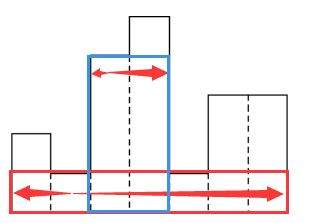
\includegraphics[width=10cm]{images/stack.png}
\end{figure}

\par \noindent 按照上述思想也能够求最大子矩形的面积。
~\\
\par \noindent 注意此做法能够优化到O(矩形1的数量),因为可以直接枚举同一行的1的位置,考虑该行相邻列都是1的情况此时计算一次答案。【按照矩形的分布计算,因为一个位置是0就可以隔断子矩形】

\begin{minted}{c++}
#include <bits/stdc++.h>

using namespace std;
const int N = 1e3 + 5;
using ll = int64_t;
int n, m, a[N][N];
int H[N][N]; // 向上最大扩展全1的长度
ll calc(int *h, int k) {//计算矩形个数 下标[0, k)
    stack<int> s;
    vector<int> l(k), r(k);
    for (int  i = k - 1; i >= 0; i--) {
        while (!s.empty() && h[i] <= h[s.top()]) l[s.top()] = i, s.pop();
        s.push(i);
    }
    while (!s.empty()) l[s.top()] = -1, s.pop();
    
    for (int  i = 0; i <= k - 1; i++) {
        while (!s.empty() && h[i] < h[s.top()]) r[s.top()] = i, s.pop();
        s.push(i);
    }
    while (!s.empty()) r[s.top()] = k, s.pop();
    ll res = 0;
    for (int  i = 0; i <= k - 1; i++)  res += (ll)h[i] * (i - l[i]) * (r[i] - i);
    return res;
}
int main() {
    scanf("%d%d", &n, &m);
    for (int i = 1; i <= n; i++) 
        for (int j = 1; j <= m; j++) 
            scanf("%d", &a[i][j]);
    ll ans = 0;
    for (int i = 1; i <= n; i++)  {
        for (int j = 1; j <= m; j++) {
            if (a[i][j])
                H[i][j] = H[i-1][j] + 1;
            else
                H[i][j] = 0;
        }
        ans += calc(H[i] + 1, m); // 每一行算一次
    }
    printf("%lld\n", ans);
    return 0;
}
/**
2 2
0 1
1 1 
子矩形数量是5
**/
\end{minted}
% 树状数组
\section{树状数组}

\par \noindent Tips: lowbit(x) => (x \& (-x)) 的含义:当 x 为 0 时,结果为 0。当 x 为奇数时,结果为 1。当 *x* 为偶数时,结果为 x 中 2 的最大次方的因子。
\subsection{区间修改,区间求和}

\par \noindent 引入差分序列,使树状数组支持区间修改。树状数组中维护的是差分序列,需要有一个数组维护原数据。
\begin{minted}{c++}
namespace Fenwick {
    int c0[maxn], c1[maxn], n;
    
    inline int lowbit(int x) { return x & (-x); }
    
    void add(int k, int v) {
      int i = k * v;
      while (k <= n) {
        c0[k] += v, c1[k] += i;
        k += lowbit(k);
      }
    }
    int sum(int k) {
      int ret = 0;
      int i = k + 1;
      while (k) {
        ret += i * c0[k] - c1[k];
        k -= lowbit(k);
      }
      return ret;
    }
    
    void modify(int l, int r, int v) {
      add(l, v), add(r + 1, -v);  // 将区间加差分为两个前缀加
    }
    
    long long query(int l, int r) {
      return sum(r) - sum(l - 1);
    }
}
\end{minted}

\subsection{三维前缀和}
\par \noindent 树状数组维护三维前缀和
\par $$\sum_{i=1}^{n}\sum_{j=1}^i\sum_{k=1}^jd_k=\frac{1}{2}[(n^2+3n+2)\sum_{i=1}^nd_i-(2n+3)\sum_{i=1}^ni·d_i+\sum_{i=1}^ni^2·d_i]$$
\par \noindent 由此也成功转化成三个一阶前缀和问题,如果继续推下去,会发现 $n$ 个树状数组就可以解决 $n$ 阶前缀和问题
\begin{minted}{c++}
namespace Fenwick {
    const int maxn = 1100;
    int c0[maxn], c1[maxn], c2[maxn];
    void add(int k, int v)
    {
        int i = k * v, ii = 1ll * k * k * v;
        while (k < maxn)
        {
            c0[k] += v;
            c1[k] += i;
            c2[k] += ii;
            k += k & -k;
        }
    }
    int sum(int k)
    {
        int ans = 0;
        int k1 = 1ll * k * k + 3 * k + 2, k2 = 2 * k + 3;
        while (k)
        {
            ans += k1 * c0[k] - k2 * c1[k] + c2[k];
            k -= k & -k;
        }
        return ans >> 1;
    }
    void modify(int l, int r, int v)
    {
        add(l, v);
        add(r + 1, -v);
    }
}
\end{minted}

\subsection{二维树状数组(矩阵求和与修改)}

\begin{minted}{c++}
namespace Fenwick_2D {
    int c0[maxn][maxn], c1[maxn][maxn], c2[maxn][maxn], c3[maxn][maxn];
    int n, m;
    inline int lowbit(int x) {
        return x & (-x);
    }
    void add(int x, int y, int v) {
        int i = x;
        while (i <= n) {
            int j = y;
            while (j <= m) {
                c0[i][j] += v;
                c1[i][j] += v * x;
                c2[i][j] += v * y;
                c3[i][j] += v * x * y;
                j += lowbit(j);
            }
            i += lowbit(i);
        }
    }
    int sum(int x, int y) {
        int ret = 0, i = x;
        while (i) {
            int j = y;
            while (j) {
                ret += c0[i][j] * (x + 1) * (y + 1);
                ret -= c1[i][j] * (y + 1);
                ret -= c2[i][j] * (x + 1);
                ret += c3[i][j];
                j -= lowbit(j);
            }
            i -= lowbit(i);
        }
        return ret;
    }
        /* 在矩形 (x0, y0),(x1, y1) 上加上 v */
    void change(int x0, int y0, int x1, int y1, int v) {
        add(x0, y0, v);
        add(x1 + 1, y0, -v);
        add(x0, y1 + 1, -v);
        add(x1 + 1, y1 + 1, v);
    }
    /* 查询矩形 (x0, y0),(x1, y1) 所有元素的和 */
    int query(int x0, int y0, int x1, int y1) {
        return sum(x1, y1) - sum(x0 - 1, y1) - sum(x1, y0 - 1) + sum(x0 - 1, y0 - 1);
    }
}using namespace Fenwick_2D;
\end{minted}
\subsection{三维树状数组}
\begin{minted}{c++}
inline int lowbit(int x) { return x & -x; }
void update(int x, int y, int z, int d) {
    for (int i = x; i <= n; i += lowbit(i))
        for (int j = y; j <= n; j += lowbit(j))
            for (int k = z; k <= n; k += lowbit(k))
                c[i][j][k] += d;
}
long long query(int x, int y, int z) {
    long long ret = 0;
    for (int i = x; i > 0; i -= lowbit(i))
        for (int j = y; j > 0; j -= lowbit(j))
            for (int k = z; k > 0; k -= lowbit(k))
                ret += c[i][j][k];
    return ret;
}
long long solve(int x0, int y0, int z0, int x1, int y1, int z1) {
    return    query(x1, y1, z1)
            - query(x1, y1, z0 - 1)
            - query(x1, y0 - 1, z1)
            - query(x0 - 1, y1, z1)
            + query(x1, y0 - 1, z0 - 1)
            + query(x0 - 1, y1, z0 - 1)
            + query(x0 - 1, y0 - 1, z1)
            - query(x0 - 1, y0 - 1, z0 - 1);
\end{minted}
% 线段树
\section{线段树}
\subsection{标记优先级}
\par \noindent 区间加、区间乘线段树

\begin{minted}{c++}
// sum = sum * mul + add * len
// add = add * mul + add
// mul = mul 
void puttag(int u, int add , int mul){
    t[u].sum = ((ll)t[u].sum * mul + (ll)(t[u].r - t[u].l + 1) * add) % mod;
    t[u].add = ((ll)t[u].add * mul + add) % mod;
    t[u].mul = (ll)t[u].mul * mul % mod;
}
void pushdown(int u){
    puttag(u << 1 , t[u].add , t[u].mul);
    puttag(u << 1 | 1 , t[u].add , t[u].mul);
    t[u].add = 0 , t[u].mul = 1;
}
// 另一种写法
// 优先级  mul > add
void mark_mul(int u, int mul) {
    t[u].sum = (ll)t[u].sum * mul % mod;
    t[u].add = (ll)t[u].add * mul % mod;
    t[u].mul = (ll)t[u].mul * mul % mod;
}
void mark_add(int u, int add) {
    t[u].sum = (t[u].sum + (ll)(t[u].r - t[u].l + 1) * add) % mod;
    t[u].add = ((ll)t[u].add + add) % mod;
}
void pushdown(int u){
    if(t[u].mul != 1) {
        mark_mul(u<<1, t[u].mul);
        mark_mul(u<<1|1, t[u].mul);
        t[u].mul = 1;
    }
    if(t[u].add) {
        mark_add(u<<1, t[u].add);
        mark_add(u<<1|1, t[u].add);
        t[u].add = 0;
    }
}
\end{minted}
\subsection{历史版本和}
\par \noindent 给定一个长度为 $n$ 的序列 $a_i$,现在有 $m$ 次操作,操作有两种:
\begin{tcolorbox}
\begin{itemize}
\item 给定区间 $[l,r]$ 和 $v$,将区间 $[l,r]$ 加上 $v$
\item 给定区间 $[l,r]$,求区间 $[l,r]$ 的历史版本和
\end{itemize}
\end{tcolorbox}
\par \noindent 用线段树维护区间和 $sum$、区间历史和 $sumh$,但是我们这里不引入时间的概念,我们将历史和 $sumh$ 看成是 $sum$ 乘上另一个标记 $tag$,而每段时间,我们手动更新 $tag$.
\par \noindent 这里认为 $tag$ 标记优先级高于加标记:
\begin{minted}{c++}
// U216697 线段树区间历史版本和 
// https://www.luogu.com.cn/problem/U216697
#include <cstdio>
#include <cstring>
#include <algorithm>
using namespace std;
using ll = long long;

const int  N = 100008;

int a[N], n, m;

struct Node {
    int len;
    ll sum, add;    //     区间和、 区间加标记
    ll sumh, addh;  // 区间历史和、历史和加标记
    ll tag;         // 次数乘上原来儿子上存的值
} t[N << 2];
void pushup(int u) {
    t[u].sum = t[u<<1].sum + t[u<<1|1].sum;
    t[u].sumh = t[u<<1].sumh + t[u<<1|1].sumh;
}
// 一起下传 考虑标记之间影响
void puttag(int u, ll add, ll addh, ll tag) {
    
    t[u].sumh += tag * t[u].sum + addh * t[u].len;
    t[u].sum += t[u].len * add;
    
    t[u].addh += tag * t[u].add + addh;
    t[u].tag += tag;
    t[u].add += add;
}
// 另一种写法
// 优先级  tag > addh > add
void puttag(int u, ll add, ll addh, ll tag) {
    t[u].sumh += tag * t[u].sum + addh * t[u].len;
    t[u].sum += t[u].len * add;
    
    t[u].addh += tag * t[u].add + addh;
    t[u].tag += tag;
    t[u].add += add;
}
void mark_tag(int u, ll tag) {
    t[u].sumh += tag * t[u].sum;
    t[u].addh += tag * t[u].add;
    t[u].tag += tag;
}
void mark_adh(int u, ll addh) {
    t[u].sumh += addh * t[u].len;
    t[u].addh += addh;
}
void mark_add(int u, ll add) {
    t[u].sum += t[u].len * add;
    t[u].add += add;
}
void pushdown(int u) {
    if (t[u].tag) {
        mark_tag(u<<1, t[u].tag);
        mark_tag(u<<1|1, t[u].tag);
        t[u].tag = 0;
    }
    if (t[u].addh) {
        mark_adh(u<<1, t[u].addh);
        mark_adh(u<<1|1, t[u].addh);
        t[u].addh = 0;
    }
    if (t[u].add) {
        mark_add(u<<1, t[u].add);
        mark_add(u<<1|1, t[u].add);
        t[u].add = 0;
    }
}
void build(int u, int l, int r) {
    t[u].len = r - l + 1;
    if (l == r) {
        t[u].sum = a[l];
        t[u].sumh = a[l];
        return;
    }
    int mid = (l + r) >> 1;
    build(u<<1, l, mid);
    build(u<<1|1, mid + 1, r);
    pushup(u);
}
void update(int u, int l, int r, int L, int R, int v) {
    if (l >= L && r <= R) {
        mark_add(u, v);
        return;
    }
    pushdown(u);
    int mid = (l + r) >> 1;
    if (L <= mid) update(u<<1, l, mid, L, R, v);
    if (R > mid) update(u<<1|1, mid + 1, r, L, R, v);
    pushup(u);
}
ll query(int u, int l, int r, int L, int R) {
    if (l >= L && r <= R) 
        return t[u].sumh;
    pushdown(u);
    int mid = (l + r) >> 1;
    ll v = 0;
    if (L <= mid) v += query(u<<1, l, mid, L, R);
    if (R > mid) v += query(u<<1|1, mid + 1, r, L, R);
    return v;
}
int main() {

    scanf("%d%d", &n, &m);
    for (int i = 1; i <= n; ++i) scanf("%d", &a[i]);
    build(1, 1, n);
    int op, x, y, l, r;
    for (int i = 1; i <= m; ++i) {
        scanf("%d", &op);
        if (op == 1) {
            scanf("%d%d%d", &l, &r, &x);
            update(1, 1, n, l, r, 1ll * x);
        }
        else {
            scanf("%d%d", &x, &y);
            printf("%lld\n", query(1, 1, n, x, y));
        }
        mark_tag(1, 1);
    }
    return 0;
}
\end{minted}
\begin{tcolorbox}
\par \noindent 给出一个长度为 $n$ 的序列 $a$,每次询问一个区间 $[l,r]$。询问有多少个子区间 $[i,j]$ 满足子区间内不同的数的数量是奇数。
\end{tcolorbox}
\begin{itemize}
\item 将询问离线,从左往右扫描右端点 $r$
\item 线段树每个点 $i$ 维护的是 $[i,r]$ 这个段区间不同数的个数是偶数/奇数
\item 那么对于区间询问 $[L, R]$ 得到的结果: 有多少形如 $[(L\to R), r]$ 区间不同数的个数是 偶数/奇数
\end{itemize}
\textbf{注意:$[(L\to R), r]$ 的区间左端点在 $[L,R]$ 右端点始终是目前扫描到的 $r$ }
~\\
\par \noindent 对于维护 $[L,R]$ 子区间 显然是维护所有答案的历史版本和!
~\\

\par \noindent \textbf{有时维护很多标记时,标记之间的关系非常混乱,考虑是否能用矩阵的形式代替。}
~\\
\par \noindent 考虑维护:

\begin{itemize}
\item 区间长度:$len=r-l+1$
\item 区间和:$sum$
\item 历史区间和:$sumh$
\end{itemize}

\par \noindent 考虑每次区间加 $val$,那么考虑各个数字的变化:

\begin{itemize}
\item 对于区间和变化量: $len×val$
\item 对于区间历史和变化量:$sum+len×val$
\end{itemize}

\par \noindent 于是有:

\begin{itemize}
\item $len = len$
\item $sum = sum + len × val$
\item $sumh = sumh + sum + len × val$
\end{itemize}

\par \noindent 把上面的式子整理一下,就可以用矩阵乘法维护(建议维护行向量用右乘矩阵)。
\begin{minted}{c++}
// U216697 线段树区间历史版本和 
// https://www.luogu.com.cn/problem/U216697
#include <bits/stdc++.h>

using namespace std;
using ll = long long;
const int  N = 100008;
int a[N], n, m;
struct Mat{
    static const int M = 3;
    ll m[M][M];
    Mat() { memset(m ,0 ,sizeof(m)); }
    Mat(ll k){
        memset(m ,0 ,sizeof(m)); 
        m[0][0] = m[1][1] = m[2][2]  = 1;
        m[0][1] = m[0][2] = k;
        m[1][2] = 1;
    }
    void eye() { for(int i = 0; i < M; i++) for(int j = 0; j < M; j++) m[i][j] = (ll)(i == j); }
    Mat operator * (const Mat& B) const{
        const Mat &A = *this;
        Mat ret;
        for(int k = 0; k < M; k++){
            for(int i = 0; i < M; i++)
                for(int j = 0; j < M; j++){
                    ret.m[i][j] = ret.m[i][j] + A.m[i][k] * B.m[k][j];
            }
        }
        return ret;
    }
    Mat operator + (const Mat& B) const{
        const Mat &A = *this;
        Mat ret;
        for(int i = 0; i < M; i++)
            for(int j = 0; j < M; j++)
                ret.m[i][j] = A.m[i][j] + B.m[i][j];
        return ret;
    }
};

struct Node {
    Mat v,tag;
} t[N << 2];
void pushup(int u) {
    t[u].v = t[u<<1].v + t[u<<1|1].v;
}
void build(int u, int l, int r) {
    t[u].tag.eye();
    if (l == r) {
        t[u].v.m[0][0] = 1;
        t[u].v.m[0][1] = a[l];
        t[u].v.m[0][2] = a[l];
        return;
    }
    int mid = (l + r) >> 1;
    build(u<<1, l, mid);
    build(u<<1|1, mid + 1, r);
    pushup(u);
}
void puttag(int u, Mat v) {
    t[u].v = t[u].v * v;
    t[u].tag = t[u].tag * v;
}
void pushdown(int u) {
    puttag(u<<1, t[u].tag);
    puttag(u<<1|1, t[u].tag);
    t[u].tag.eye();
}
void update(int u, int l, int r, int L, int R, ll v) {
    if (l >= L && r <= R) {
        puttag(u, Mat(v));
        return;
    }
    pushdown(u);
    int mid = (l + r) >> 1;
    if (L <= mid) update(u<<1, l, mid, L, R, v);
    if (R > mid)  update(u<<1|1, mid + 1, r, L, R, v);
    pushup(u);
}

Mat query(int u, int l, int r, int L, int R) {
    if (l >= L && r <= R) return t[u].v;
    
    pushdown(u);
    int mid = l + r >> 1;
    Mat ret;
    if (L <= mid) ret = ret + query(u<<1, l, mid, L, R);
    if (R > mid)  ret = ret + query(u<<1|1, mid + 1, r, L, R);
    return ret;
}

int main() {

    scanf("%d%d", &n, &m);
    for (int i = 1; i <= n; ++i) scanf("%d", &a[i]);
    build(1, 1, n);
    int op, x, y, l, r;
    for (int i = 1; i <= m; ++i) {
        scanf("%d", &op);
        if (op == 1) {
            scanf("%d%d%d", &l, &r, &x);
            update(1, 1, n, l, r, x);
            if(l - 1 >= 1)update(1, 1, n, 1, l - 1, 0);
            if(r + 1 <= n)update(1, 1, n, r + 1, n, 0);
        }
        else {
            scanf("%d%d", &x, &y);
            printf("%lld\n", query(1, 1, n, x, y).m[0][2]);
            update(1, 1, n, 1, n, 0);
        }
    }
    return 0;
}
\end{minted}
\subsection{不降子序列}
\par \noindent 线段树维护以某点为开头的最长不下降子序列,使用下面calc函数能够计算线段树\textbf{u维护的区间中},以$x$ 为开头最长不下降子序列的个数。calc需要维护区间最值。

\begin{minted}{c++}
template<typename T>
int calc(int u,T x)
{
    if(t[u].l==t[u].r) 
        return t[u].v>x?1:0;
    if(t[u<<1].v<=x) 
        return calc(u<<1|1,x);
    return t[u].cnt-t[u<<1].cnt+calc(u<<1,x);
}
\end{minted}

\subsection{维护矩阵}
\begin{tcolorbox}
\par \noindent 维护三个长度为 $n$ 的序列 $A, B, C$ ,支持以下 7 种操作:$n, m \leq 2.5 \times 10^5, 0 \leq A_{i}, B_{i}, C_{i}<998244353$
\begin{enumerate}
\item $l, r$ : 对 $[l, r], A_{i} \leftarrow A_{i}+B_{i}$
\item $l, r$ : 对 $[l, r],  B_{i} \leftarrow B_{i}+C_{i}$
\item $l, r$ : 对 $[l, r], C_{i} \leftarrow C_{i}+A_{i}$ 
\item $l, r,v$ : 对 $[l, r],  A_{i} \leftarrow A_{i}+v$
\item $l, r,v$ : 对 $[l, r],   B_{i} \leftarrow B_{i} \cdot v$ 
\item $l, r,v$ : 对 $[l, r],   C_{i} \leftarrow v$
\item $l,r$ : 求 $\sum_{i=l}^{r} A_{i}, \sum_{i=l}^{r} B_{i}, \sum_{i=l}^{r} C_{i}$ 在模 998244353 意义下。 
\end{enumerate}
\end{tcolorbox}
\begin{minted}{c++}
#include <bits/stdc++.h>
using namespace std;
typedef long long ll;
const int N = 250010;

const ll mod = 998244353;
struct dat {
    int n, m;
    ll a[5][5];
    dat() {}
    dat(int _n, int _m) {
        n = _n;
        m = _m;
        memset(a, 0, sizeof a);
    }
    friend dat operator +(const dat &X, const dat &Y) {
        //assert(X.n==Y.n);
        //assert(X.m==Y.m);
        dat ret(X.n, X.m);

        for (int i = 1; i <= X.n; i++)
            for (int j = 1; j <= X.m; j++)
                ret.a[i][j] = (X.a[i][j] + Y.a[i][j]) % mod;

        return ret;
    }
    friend dat operator *(const dat &X, const dat &Y) {
        dat ret(X.n, Y.m);
        assert(X.m == Y.n);
        for (int i = 1; i <= X.n; i++)
            for (int j = 1; j <= Y.m; j++)
                for (int k = 1; k <= X.m; k++)
                    ret.a[i][j] = (ret.a[i][j] + X.a[i][k] * Y.a[k][j]) % mod;
        return ret;
    }
};
struct node {
    int l, r;
    dat v, tag;
} t[N << 2];

int n, m;
dat num[N];
dat base1, base2, base3, base4, base5, base6;
dat base;
void build(int u, int l, int r) {
    t[u].l = l, t[u].r = r;
    if (l == r) {
        t[u].v = num[l];
        t[u].tag = base;
        return;
    }
    int mid = l + r >> 1;
    build(u << 1, l, mid), build(u << 1 | 1, mid + 1, r);
    t[u].v = t[u << 1].v + t[u << 1 | 1].v;
    t[u].tag = base;
}
void put(int u, dat &v) {
    t[u].v = t[u].v * v;
    t[u].tag = t[u].tag * v;
}
void pushdown(int u) {
    put(u << 1, t[u].tag);
    put(u << 1 | 1, t[u].tag);
    t[u].tag = base;
}
void modify(int u, int l, int r, dat v) {
    if (l <= t[u].l && t[u].r <= r) {
        t[u].v = t[u].v * v;
        t[u].tag = t[u].tag * v;
        return;
    }
    pushdown(u);
    int mid = t[u].l + t[u].r >> 1;
    if (l <= mid) modify(u << 1, l, r, v);
    if (r > mid) modify(u << 1 | 1, l, r, v);
    t[u].v = t[u << 1].v + t[u << 1 | 1].v;
}
dat query(int u, int l, int r) {
    if (l <= t[u].l && t[u].r <= r)
        return t[u].v;
    pushdown(u);
    int mid = t[u].l + t[u].r >> 1;
    dat v(1, 4);
    if (l <= mid) v = v + query(u << 1, l, r);
    if (r > mid) v = v + query(u << 1 | 1, l, r);
    return v;
}

void init() {
    base = dat(4, 4);
    for (int i = 1; i <= 4; i++)
        base.a[i][i] = 1;

    /*
    base1:| base2:| base3:
    1 0 0 | 1 0 0 | 1 0 1
    1 1 0 | 0 1 0 | 0 1 0
    0 0 1 | 0 1 1 | 0 0 1
    */
    base1 = base;
    base1.a[2][1] = 1;
    base2 = base;
    base2.a[3][2] = 1;
    base3 = base;
    base3.a[1][3] = 1;
    /*
    base4:  | base5:  | base6:
    1 0 0 0 | 1 0 0 0 | 1 0 0 0
    0 1 0 0 | 0 v 0 0 | 0 1 0 0
    0 0 1 0 | 0 0 1 0 | 0 0 0 0
    v 0 0 1 | 0 0 0 1 | 0 0 v 1
    */
    base4 = base; // [4][1]=v
    base5 = base; // [2][2]=v;
    // [4][3]=v;
    base6 = base;
    base6.a[3][3] = 0;
}


int main() {
    init();
    cin >> n;
    for (int i = 1; i <= n; i++) {
        num[i] = dat(1, 4);
        cin >> num[i].a[1][1] >> num[i].a[1][2] >> num[i].a[1][3];
        num[i].a[1][4] = 1;
    }
    build(1, 1, n);
    cin >> m;

    while (m--) {
        int op, l, r, v;
        cin >> op >> l >> r;
        if (op == 1)
            modify(1, l, r, base1);
        else if (op == 2)
            modify(1, l, r, base2);
        else if (op == 3)
            modify(1, l, r, base3);
        else if (op == 4) {
            cin >> v;
            base4.a[4][1] = v;
            modify(1, l, r, base4);
        } else if (op == 5) {
            cin >> v;
            base5.a[2][2] = v;
            modify(1, l, r, base5);
        } else if (op == 6) {
            cin >> v;
            base6.a[4][3] = v;
            modify(1, l, r, base6);
        } else {
            dat ret = query(1, l, r);
            cout << ret.a[1][1] << ' ' << ret.a[1][2] << ' ' << ret.a[1][3] << '\n';
        }
    }

    return 0;
}
\end{minted}
\subsection{区间 GCD}

\begin{tcolorbox}
给定一个长度为 N 的数列 A,以及 M 条指令,每条指令可能是以下两种之一:
\begin{itemize}
\item C l r d,表示把 $A[l],A[l+1],…,A[r]$ 都加上 $d$。
\item Q l r,表示询问 $A[l],A[l+1],…,A[r]$ 的最大公约数。
\end{itemize}
\end{tcolorbox}

$$
\operatorname{gcd}\left(a_1, a_2, \cdots, a_n\right)=\operatorname{gcd}\left(a_1, a_2-a_1, a_3-a_2, \cdots, a_n-a_{n-1}\right)
$$

\par \noindent 根据性质用 $b[i] = a[i] - a[i-1]$数组,表示原序列的差分序列,用线段数维护 $b[i]$ 的区间的最大公约数
\begin{itemize}
\item 询问 C l r d  等价于
\begin{enumerate}
\item $b[l]$ 加上 $d$、$b[r+1]$ 减去 $d$ ,只需两次线段数的单点修改即可
\item 对于原序列中 $a[i]$ 的值,需要支持区间加、点单查询,只需要用树状数组通过维护差分序列即可。
\end{enumerate}
\item 询问 Q l r 等于求出 $\operatorname{gcd}(a[l]$, query $(1, l+1, r))$
\end{itemize}
\begin{minted}{c++}
#include<bits/stdc++.h>

using namespace std;
using ll = long long;
const int N = 500010;

int n, m;
ll a[N];
struct Node {
    int l, r;
    ll v;
}t[N<<2];
void pushup(int u) {
    t[u].v = __gcd(t[u << 1].v, t[u << 1 | 1].v);
}
void build(int u, int l, int r) {
    t[u]={l, r};
    if (l == r) {
        t[u].v = a[l] - a[l - 1];
        return;
    }
    int mid = l + r >> 1;
    build(u << 1, l, mid);
    build(u << 1 | 1, mid + 1, r);
    pushup(u);
}
void modify(int u, int pos, ll x) {
    if(t[u].l == t[u].r) {
        t[u].v += x;
        return;
    }
    int mid = t[u].l + t[u].r >> 1;
    if(pos <= mid) modify(u << 1, pos, x);
    else modify(u << 1 | 1, pos, x);
    pushup(u);
}
ll query(int u, int l, int r) {
    if(l <= t[u].l && t[u].r <=r) {
        return t[u].v;
    }
    int mid = t[u].l + t[u].r >> 1;
    ll v = 0;
    if(l <= mid) v = __gcd(v, query(u << 1, l, r));
    if(r > mid) v = __gcd(v, query(u << 1 | 1, l, r));
    return v;
}

ll bit[N];
void add(int k, ll x) {
    for(; k <= n; k += k&-k) bit[k] += x;
}
ll sum(int k) {
    ll v = 0;
    for(; k; k -= k&-k) v += bit[k];
    return v;
}
int main() {

    cin >> n >> m;
    for (int i = 1; i <= n; i++) cin >> a[i];
    // 差分数组
    build(1, 1, n);

    // 原数组 -> 树状数组差分维护
    for (int i = 1; i <= n; i ++) add(i, a[i] - a[i-1]);

    while (m--) {
        char op;
        int l, r; 
        cin >> op >> l >> r;
        if (op =='Q') {
            ll x = sum(l);
            ll y = query(1, l + 1, r);
            cout << abs(__gcd(x, y)) << '\n';
        }
        else {
            ll val; cin >> val;
            // 原数组 区间加
            add(l, val);
            if(r + 1 <= n) add(r + 1, -val);
            // 差分数组
            modify(1, l, val);
            if (r + 1 <= n) modify(1, r + 1, -val);
        }
    }

    return 0;
}
\end{minted}


有时候维护集合的 gcd 并支持:
\begin{enumerate}
\item 合并两个 gcd 集合
\item 对某些集合的所有数加上一个值
\end{enumerate}
$$
\operatorname{gcd}\left(a_1, a_2, \cdots, a_n\right)=\operatorname{gcd}\left(a_1, a_2-a_1, a_3-a_1, \cdots, a_n-a_{1}\right)
$$

\par \noindent 对于每一个集合维护两个数 
$$
f = a_1,g = \gcd(a_2-a_1, a_3-a_1, \cdots, a_n-a_{1})
$$
\par \noindent 对一个集合的所有数加上一个值操作 $f$ 即可。下面考虑如何合并两个集合:
~\\
\par \noindent 两个 gcd 合并时 需要将 $f_1$ 和 $f_2$ 合并 $g_1$ 和 $g_2$ 合并,令 $f_1$ 和 $f_2$ 合并成 $f_1$ (意味着对于两个序列合并,维护第一个序列的$a_1$)考虑差分的性质,对第二个集合来说等价于所有数减去 $f_1$,于是合并后集合应该有:
$$
f = f_1, g = \gcd(g_1, g_2,f_2 -f_1)
$$
\subsection{区间NAND}

\par \noindent 区间与非\textbf{没有结合律},这样的信息线段树不能直接维护,不过位运算具有独立性,我们可以一位一位去考虑。
~\\
\par \noindent 考虑用线段树每个节点维护$\text{L}[0/1],\text{R}[0/1]$
\begin{itemize}
\item $\text{L}[0]$表示刚开是$0$,然后从左向右经过此区间是最终的数(此节点维护的区间)
\item $\text{L}[1]$表示刚开是$1$,然后从左向右经过此区间是最终的数
\item $\text{R}[0]$表示刚开是$0$,然后从右向左经过此区间是最终的数
\item $\text{R}[1]$表示刚开是$1$,然后从右向左经过此区间是最终的数
\end{itemize}
\par \noindent 然后只需要维护32棵线段树(按位),就可以区间询问了。而且区间是从左向右,有的区间是从右向左的答案也不一样!

\begin{minted}{c++}
struct Segment
{
    struct node
    {
        int l,r;
        bool L[2],R[2];
    }tree[N<<2];
    void pushup(int u)
    {
        tree[u].L[0]=tree[u<<1|1].L[tree[u<<1].L[0]];
        tree[u].L[1]=tree[u<<1|1].L[tree[u<<1].L[1]];
        tree[u].R[0]=tree[u<<1].R[tree[u<<1|1].R[0]];
        tree[u].R[1]=tree[u<<1].R[tree[u<<1|1].R[1]];
    }
    void build(int u,int l,int r,int k)
    {
        tree[u].l=l,tree[u].r=r;
        if(l==r) 
        {
            tree[u].L[0]=tree[u].R[0]=1;
            tree[u].L[1]=tree[u].R[1]=!(a[id[l]]>>k&1);
            return;
        }
        int mid=l+r>>1;
        build(u<<1,l,mid,k);build(u<<1|1,mid+1,r,k);
        pushup(u);
    }
    void modify(int u,int pos,bool x)
    {
        if(tree[u].l==tree[u].r)
        {
            tree[u].L[0]=tree[u].R[0]=1;
            tree[u].L[1]=tree[u].R[1]=(!x);
            return;
        }
        int mid=tree[u].l+tree[u].r>>1;
        if(pos<=mid) 
            modify(u<<1,pos,x);
        else
            modify(u<<1|1,pos,x);
        pushup(u);
    }
    bool queryL(int u,int l,int r,bool c)
    {
        if(l<=tree[u].l&&tree[u].r<=r) return tree[u].L[c];
        int mid=tree[u].l+tree[u].r>>1;
        if(r<=mid)
            return queryL(u<<1,l,r,c);
        else if(l>mid) 
            return queryL(u<<1|1,l,r,c);
        else 
            return queryL(u<<1|1,l,r,queryL(u<<1,l,r,c));
        
    }
    bool queryR(int u,int l,int r,bool c)
    {
        if(l<=tree[u].l&&tree[u].r<=r) return tree[u].R[c];
        int mid=tree[u].l+tree[u].r>>1;
        if(r<=mid)
            return queryR(u<<1,l,r,c);
        else if(l>mid) 
            return queryR(u<<1|1,l,r,c);
        else 
            return queryR(u<<1,l,r,queryR(u<<1|1,l,r,c));
    }
}T[33];
\end{minted}
\subsection{主席树}
\par \noindent 可持久化线段树的主要思想:保存每次插入操作的历史版本,实际上是在动态开点线段树的基础上,通过复用某些未修改的节点,创建 $n$ 棵线段树。
~\\
\par \noindent 每进行一次修改时,产生新的节点数 = 树的高度,是$O(n \log n)$ 级别的。

\begin{minted}{c++}
struct node
{
    int l,r;
    ll v;
}t[N*40];
int rt[N],cnt;
void ins(int &u,int o,int l,int r,int pos)
{
    u=++cnt;
    t[u]=t[o];
    t[u].v+=pos;
    if(l==r) return;
    int mid=l+r>>1;
    if(pos<=mid) 
        ins(t[u].l,t[o].l,l,mid,pos);
    else
        ins(t[u].r,t[o].r,mid+1,r,pos);
}
ll query(int u,int l,int r,int L,int R)
{
    if(!u) return 0ll;
    if(L<=l&&r<=R) return t[u].v;
    int mid=l+r>>1;
    ll v=0;
    if(L<=mid)   
        v+=query(t[u].l,l,mid,L,R);
    if(R>mid)
        v+=query(t[u].r,mid+1,r,L,R);
    return v;
}
\end{minted}

\subsection{动态开点权值线段树}
\par \noindent 有的时候,线段树需要维护的区间很大很大,但是实际用到的节点很少;那么干脆就不要开这么多的节点,用到的时候再向内存要。

\begin{minted}{c++}
namespace DynamicSegTree {
    struct Node {
        int l, r, v;
    }t[maxn*40];
    int cnt;
    // 修改操作,若 u 不存在,则首先动态开点;否则直接更新
    void update(int &u, int l, int r, int pos, int val) {
        if(!u) u = ++cnt;
        // ....
    }
    // 查询操作区间 [L, R] ,若 u 不存在直接返回空值(可能是 0 或者反向最值)
    int query(int u, int l, int r, int L, int R) {
        if(!u) 
            return 0;
        // .....
    }

}using namespace DynamicSegTree;
\end{minted}
\subsection{线段树合并}
\begin{minted}{c++}
int merge(int x,int y,int l,int r)
{
    if(!x||!y) return x+y;
    int mid=l+r>>1;
    if(l==r)
    {
        t[x].val+=t[y].val;
        return x;
    }
    t[x].l=merge(t[x].l,t[y].l,l,mid);
    t[x].r=merge(t[x].r,t[y].r,mid+1,r);
    t[x].val=max(t[t[x].l].val,t[t[x].r].val);
    return x;
}
\end{minted}

\subsection{Segment Tree Beats!}
\par \noindent 区间最值操作往往采用以下办法 

\par \noindent 线段树维护:
\begin{itemize}
\item 区间最大值$\text{mx}$  
\item 区间严格次大值$\text {smx}$  
\item 区间和$\text{sum}$ 
\item 区间最大值个数$\text{cnt}$  
\item 区间最值懒标记$\text{lazy}$
\end{itemize}
\par \noindent 实现区间最小值操作,考虑u节点维护的区间,进行如下处理
\begin{itemize}
\item 当$\text{mx}\leq x$,显然这次修改不会对这个节点维护的区间产生影响,直接退出。
\item 当$\text{smx}<x<\text{mx}$,显然这次修改只会影响到这个区间所有的最大值,由此直接根据最大值个数更新区间和并且更新区间最大值并打上懒标记然后退出即可。
\item 当$\text{x}\leq \text{smx}$,无法直接更新于是递归左右子树。
\end{itemize}

\begin{minted}{c++}
struct Node {
    int l, r; // 最大值 次大值 区间和
    ll maxv, secmaxv, sum;
    int cnt;
    ll tag;
} t[N << 2];
int n, m;
ll a[N];
void pushup(int u) {
    int x = u << 1, y = u << 1 | 1;
    t[u].sum = t[x].sum + t[y].sum;
    // 保证 t[x].maxv > t[u].maxv
    if (t[x].maxv < t[y].maxv) swap(x, y);
    
    if (t[x].maxv != t[y].maxv) {
        t[u].maxv = t[x].maxv;
        t[u].secmaxv = max(t[x].secmaxv, t[y].maxv);
        t[u].cnt = t[x].cnt;
    } else {
        t[u].maxv = t[x].maxv;
        t[u].secmaxv = max(t[y].secmaxv, t[y].secmaxv);
        t[u].cnt = t[x].cnt + t[y].cnt;
    }
}
void puttag(int u, ll x) {
    if (t[u].maxv <= x) return;
    t[u].sum += (x - t[u].maxv) * t[u].cnt;
    t[u].maxv = t[u].tag = x;
}
void pushdown(int u) {
    if (t[u].tag == -1) return;
    puttag(u << 1, t[u].tag), puttag(u << 1 | 1, t[u].tag);
    t[u].tag = -1;
}
void build(int u, int l, int r) {
    t[u] = {l, r, 0, -1, 0, 0, -1};
    if (l == r) {
        t[u].maxv = t[u].sum = a[l];
        t[u].cnt = 1;
        return;
    }
    int mid = l + r >> 1;
    build(u << 1, l, mid), build(u << 1 | 1, mid + 1, r);
    pushup(u);
}
void modify(int u, int l, int r, ll x) { // 区间[l, r] a[i] = min(a[i], x)
    if (x >= t[u].maxv) return;
    // 当修改只会影响到区间最大值,并且不影响次大值时修改 意味着 secmaxv < x < maxv
    // 此时需要把区间最大值修改成 x
    if (t[u].l >= l && t[u].r <= r && t[u].secmaxv < x) {
        puttag(u, x);
        return;
    }
    pushdown(u);
    int mid = t[u].l + t[u].r >> 1;
    if (l <= mid) modify(u << 1, l, r, x);
    if (r > mid) modify(u << 1 | 1, l, r, x);
    pushup(u);
}
ll qmax(int u, int l, int r) {
    if (t[u].l >= l && t[u].r <= r) return t[u].maxv;
    int mid = t[u].r + t[u].l >> 1;
    pushdown(u);
    ll v = -1;
    if (l <= mid) v = max(v, qmax(u << 1, l, r));
    if (r > mid) v = max(v, qmax(u << 1 | 1, l, r));
    pushup(u);
    return v;
}
ll qsum(int u, int l, int r) {
    if (t[u].l >= l && t[u].r <= r)
        return t[u].sum;
    int mid = t[u].r + t[u].l >> 1;
    pushdown(u);
    ll v = 0;
    if (l <= mid) v += qsum(u << 1, l, r);
    if (r > mid) v += qsum(u << 1 | 1, l, r);
    pushup(u);
    return v;
}
\end{minted}

\begin{tcolorbox}
\par \noindent 维护一个长度为 $n$ 的序列,支持 $m$ 次操作,操作包括区间按位或一个数,区间按位与一个数,以及查询区间最大值。
\end{tcolorbox}

\par \noindent 线段树每个节点上维护区间与、区间或和区间最大值。
如果一次操作对区间与的影响和对区间或的影响相同,那么就说明对这整个区间的影响都是相同的,就是加上或减去同一个值,直接打标记即可,否则递归下去处理。

% 树套树
\section{树套树}

\subsection{树状数组套权值线段树}

\par \noindent 二维数颜色

\begin{minted}{c++}
#include <bits/stdc++.h>
using namespace std;
template <class T = int> T rd() {
    T res = 0;
    char ch = getchar();
    while (!isdigit(ch)) ch = getchar();
    while (isdigit(ch)) res = (res << 1) + (res << 3) + (ch ^ 48), ch = getchar();
    return res;
}
const int N = 100010;
int a[N], n, m, ans[N], last[N];
struct nodeq {
    int l, L, R, id;
};
vector<nodeq> q[N];
struct node {
    int l, r, v;
} tree[N * 200];
int rt[N], cnt, lim;
void update(int &u, int l, int r, int pos, int v) {
    if (!u)
        u = ++cnt;

    tree[u].v += v;

    if (l == r)
        return;

    int mid = l + r >> 1;

    if (pos <= mid)
        update(tree[u].l, l, mid, pos, v);

    if (pos > mid)
        update(tree[u].r, mid + 1, r, pos, v);

    //tree[u].v=tree[tree[u].l].v+tree[tree[u].r].v;
}
int query(int u, int l, int r, int L, int R) {
    if (!u)
        return 0;

    if (L <= l && r <= R) return tree[u].v;

    int mid = l + r >> 1;
    int v = 0;

    if (L <= mid) v += query(tree[u].l, l, mid, L, R);
    if (R > mid) v += query(tree[u].r, mid + 1, r, L, R);
    return v;
}
/* 树状数组 */
// rt[i] 保存每个单点对应的权值线段树根节点,
int lowbit(int x) { return x & -x; }
void add(int k, int pos, int v) {
    for (; k <= n; k += lowbit(k)) update(rt[k], 0, lim, pos, v);
}
int ask(int k, int L, int R) {
    int ans = 0;
    for (; k; k -= lowbit(k)) ans += query(rt[k], 0, lim, L, R);
    return ans;
}
int main() {
    n = rd(), m = rd();

    for (int i = 1; i <= n; i++) a[i] = rd();

    lim = *max_element(a + 1, a + 1 + n);

    for (int i = 1; i <= m; i++) {
        int x0 = rd(), y0 = rd(), x1 = rd(), y1 = rd();
        q[x1].push_back({x0, y0, y1, i});
    }
    for (int i = 1; i <= n; i++) {
        if (last[a[i]]) add(last[a[i]], a[i], -1);

        add(i, a[i], 1);
        last[a[i]] = i;
        for (auto t : q[i]) ans[t.id] = ask(i, t.L, t.R) - ask(t.l - 1, t.L, t.R);
    }
    for (int i = 1; i <= m; i++) printf("%d\n", ans[i]);

}
\end{minted}

\subsection{下标线段树套(值域)平衡树}
\par \noindent 首先,对于维护值域的平衡树通常可以采用\textbf{权值线段树}代替。
~\\
\par \noindent 但是一般情况下,平衡树维护值域时,下标信息就会丢失,意味着不能维护类似下表是第 $i$ 个数是谁(除非开数组记录),因此也就不能维护区间 $[l,r]$ 内某个数的排名前驱后继等操作。
~\\
\par \noindent 想要维护同时维护下标,必须外层用一个数据结构维护下标,比如可以采用(下标)线段树套(值域)平衡树。此时便可以支持同时维护【下标】和【值域】的操作。
~\\
\begin{enumerate}
\item \textbf{查询 $k$ 在区间 $[l,r]$ 的排名:}找到下标线段树上 $[l,r]$ 所对应的 $\log N$个终止结点,统计每个结点平衡树内 $<k$元素个数,求和 $+1$ 就是 $k$ 的排名,复杂度$O(n\log^2n)$。
\item \textbf{查询区间 $[l,r]$ 内排名为 $k$ 的值:}二分答案然后用Getrank判断,复杂度$O(n\log^3n)$。
\item \textbf{修改某一位值上的数值 $a[i]=x$:}只要在所有包含 $a[i]$ 的平衡树($\log N$个)中删除 $a[i]$,然后再插入 $x$ 即可,复杂度$O(n\log^2n)$。
\item \textbf{查询 $x$ 在区间内 $[l,r]$ 的前驱:}在 $[l,r]$ 的所有终止结点的平衡树内查询前驱,取所有中止节点前驱的最大值,复杂度$O(n\log^2n)$。
\item \textbf{查询 $x$ 在区间内 $[l,r]$ 的后继:}在 $[l,r]$ 的所有终止结点的平衡树内查询后继,取所有中止节点后继的最小值,复杂度 $O(n\log^2n)$。
\end{enumerate}

\begin{minted}{c++}
#include<bits/stdc++.h>

using namespace std;
const int N = 50010;
const int seed = []() {
    random_device rds;
    return rds();
}();
mt19937 rd(seed);
// Treap 维护值域
struct T {
        const int key;      // 随机值 满足堆的性质
        int ls, rs, sz;     // 基本值数量  该题没用
        int val;            // 维护序列的值
        T() : key(rd()) {
            ls = rs = 0;
            sz = 0;
            val = 0;
        }
}t[N * 40];
int cnt;
// 无旋Treap平衡树 一个Treap只需要知道根节点是谁即可
struct Treap {
    int rt;
    int newnode(int x) {
        t[++cnt].val = x;
        t[cnt].sz = 1;
        return cnt;
    }
    void pushup(int u) {
        t[u].sz = t[t[u].ls].sz + t[t[u].rs].sz + 1;
    }
    // 两棵树合并
    int merge(int x, int y) {
        if (!x || !y) {
            return x | y;
        }
        int u = 0;
        if (t[x].key < t[y].key) {
            u = x, t[u].rs = merge(t[u].rs, y);
        } else {
            u = y, t[u].ls = merge(x, t[u].ls);
        }
        pushup(u);
        return u;
    }
    // 按val分裂 分裂出 <= val 的部分
    void split(int u, int val, int &x, int &y) {
        if (!u) {
            x = y = 0;
            return;
        }
        if (t[u].val <= val) {
            x = u;
            split(t[u].rs, val, t[x].rs, y);
        }
        else {
            y = u;
            split(t[u].ls, val, x, t[y].ls);
        }
        pushup(u);
    }
    // 分裂出 <= val 的部分
    pair<int, int> split(int u, int val) {
        int x, y;
        split(u, val, x, y);
        return make_pair(x, y);
    }
    void ins(int val) {
        auto [x, y] = split(rt, val);
        rt = merge(merge(x, newnode(val)), y);
    }
    void del(int val) {
        auto [w, z] = split(rt, val);
        auto [x, y] = split(w, val - 1);
        y = merge(t[y].ls, t[y].rs); // 删去一个点相当于合并
        rt = merge(merge(x, y), z);
    }
    // val的排名 = 小于val的个数 + 1
    int getrank(int val) {
        auto [x, y] = split(rt, val - 1);
        int cnt = t[x].sz + 1;
        rt = merge(x, y);
        return cnt;
    }
    // 排名时 k 的值
    int getval(int k) {
        int u = rt;
        while(u) {
            if(t[t[u].ls].sz + 1 == k) break;
            else if(t[t[u].ls].sz >= k) u = t[u].ls;
            else {
                k -= t[t[u].ls].sz + 1;
                u = t[u].rs;
            }
        }
        return t[u].val;
    }
    int pre(int val) {
        auto [x, y] = split(rt, val - 1);
        int u = x;
        while(t[u].rs) u = t[u].rs;
        rt = merge(x, y);
        return u ? t[u].val : -2147483647;
    }
    int suc(int val) {
        auto [x, y] = split(rt, val);
        int u = y;
        while(t[u].ls) u = t[u].ls;
        rt = merge(x, y);
        return u ? t[u].val : 2147483647;
    }
};
int n, m;
int a[N];
// 线段树
struct Node {
    int l, r;
    Treap treap;
}tree[N << 2];

void build(int u, int l, int r) {
    tree[u].l = l, tree[u].r = r;

    for (int i = l; i <= r; i++) tree[u].treap.ins(a[i]);

    if (l == r) return;

    int mid = l + r >> 1;
    build(u << 1, l, mid); build(u << 1 | 1, mid + 1, r);
}
void modify(int u, int pos, int x) {
    tree[u].treap.del(a[pos]);
    tree[u].treap.ins(x);

    if (tree[u].l == tree[u].r)
        return;

    int mid = tree[u].l + tree[u].r >> 1;

    if (pos <= mid)
        modify(u << 1, pos, x);
    else
        modify(u << 1 | 1, pos, x);
}
int Getrank(int u, int l, int r, int val) {
    if (l <= tree[u].l && tree[u].r <= r)
        return tree[u].treap.getrank(val) - 1;

    int mid = tree[u].l + tree[u].r >> 1;
    int k = 0;

    if (l <= mid)
        k += Getrank(u << 1, l, r, val);

    if (r > mid)
        k += Getrank(u << 1 | 1, l, r, val);

    return k;
}
int Getval(int u, int l, int r, int k) {
    int vl = 0, vr = 1e8;

    while (vl < vr) {
        int mid = vl + vr + 1 >> 1;

        if (Getrank(u, l, r, mid) + 1 <= k)
            vl = mid; //注意二分 需要二分排名<=k的最大数(数可能重复)
        else
            vr = mid - 1;
    }

    return vl;
}
int Getpre(int u, int l, int r, int val) {
    if (tree[u].l >= l && tree[u].r <= r)
        return tree[u].treap.pre(val);

    int mid = tree[u].l + tree[u].r >> 1;

    if (r <= mid)
        return Getpre(u << 1, l, r, val);
    else if (l > mid)
        return Getpre(u << 1 | 1, l, r, val);
    else
        return max(Getpre(u << 1, l, r, val), Getpre(u << 1 | 1, l, r, val));
}
int Getsuc(int u, int l, int r, int val) {
    if (tree[u].l >= l && tree[u].r <= r)
        return tree[u].treap.suc(val);

    int mid = tree[u].l + tree[u].r >> 1;

    if (r <= mid)
        return Getsuc(u << 1, l, r, val);
    else if (l > mid)
        return Getsuc(u << 1 | 1, l, r, val);
    else
        return min(Getsuc(u << 1, l, r, val), Getsuc(u << 1 | 1, l, r, val));
}

int main() {
    ios::sync_with_stdio(false);cin.tie(nullptr);cout.tie(nullptr);
    cin >> n >> m;

    for (int i = 1; i <= n; i++) cin >> a[i];

    build(1, 1, n);

    while (m--) {
        int op, l, r, k;
        cin >> op;
    
        if (op == 1) {
            cin >> l >> r >> k;
            cout << Getrank(1, l, r, k) + 1 << '\n';
        } else if (op == 2) {
            cin >> l >> r >> k;
            cout << Getval(1, l, r, k) << '\n';
        } else if (op == 3) {
            cin >> l >> k;
            modify(1, l, k);
            a[l] = k;
        } else if (op == 4) {
            cin >> l >> r >> k;
            cout << Getpre(1, l, r, k) << '\n';
        } else {
            cin >> l >> r >> k;
            cout << Getsuc(1, l, r, k) << '\n';
        }
    }
    return 0;
}
\end{minted}


\subsection{值域线段树套(下标)平衡树}

\par \noindent 当然可以用\textbf{动态开点}线段树维护值域,也就是权值线段树,用平衡树维护下标
~\\
\begin{enumerate}
\item \textbf{查询 $k$ 在区间 $[l,r]$ 的排名:} 找到值域线段树上 $[0,k-1]$ 所对应的 $\log N$个终止结点,统计每个结点平衡树下标在 $[l,r]$ 区间内元素个数即求出区间为 $[l,r]$ 内值域在 $[0,k-1]$点的个数,求和+1就是 $k$ 的排名,复杂度 $O(n\log^2n)$。

\item \textbf{查询区间 $[l,r]$ 内排名为 $k$ 的值:}在值域线段树上二分,每次看值域范围 $[vl,mid]$ 中 $[L,R]$ 区间中数的个数 = tree[u].treap.query(L, R) 与 $k$ 的关系,$\ge k$ 递归左子树,否则递归右子树,复杂度 $O(n\log^2 n)$。
\item \textbf{修改某一位值上的数值 $a[i]=x$:}只要在所有包含 $a[i]$ 的平衡树($\log {|a[i]|}$个) 中删除 $a[i]$,然后再插入 $x$ 即可,复杂度 $O(n\log^2n)$。
\item \textbf{查询 $x$ 在区间内$[l,r]$ 的前驱:} 先用操作1查询 $x$ 在 $[l,r]$ 内的排名 $k$,然后再用操作2查询排名为$k-1$ 数,复杂度 $O(n\log^2n)$。
\item \textbf{查询 $x$ 在区间内 $[l,r]$ 的后继:}先用Query求出区间在 $[l,r]$ 内值域 $[0,x]$ 的个数 $k$,然后再用操作2查询排名为 $k+1$数,复杂度 $O(n\log^2n)$。
\end{enumerate}

\begin{minted}{c++}
#include <random>
#include <iostream>
#include <algorithm>
using namespace std;
const int N = 100010;
const int MINF = -2147483647, MAXF = 2147483647;
const int seed = []() {
    random_device rds;
    return rds();
}();
mt19937 rd(seed);

int n, m;
int a[N];
int Root;
// Treap 维护值域
struct T {
        const int key;      // 随机值 满足堆的性质
        int ls, rs, sz;     // 基本值数量 
        int val;            // 维护序列的值
        T() : key(rd()) {
            ls = rs = 0;
            sz = 0;
            val = 0;
        }
}t[N * 40];
int cnt;

// 无旋Treap平衡树 一个Treap只需要知道根节点是谁即可
struct Treap {
    int rt;
    int newnode(int x) {
        t[++cnt].val = x;
        t[cnt].sz = 1;
        return cnt;
    }
    void pushup(int u) {
        t[u].sz = t[t[u].ls].sz + t[t[u].rs].sz + 1;
    }
    // 两棵树合并
    int merge(int x, int y) {
        if (!x || !y) {
            return x | y;
        }
        int u = 0;
        if (t[x].key < t[y].key) {
            u = x, t[u].rs = merge(t[u].rs, y);
        } else {
            u = y, t[u].ls = merge(x, t[u].ls);
        }
        pushup(u);
        return u;
    }
    // 按val分裂 分裂出 <= val 的部分
    void split(int u, int val, int &x, int &y) {
        if (!u) {
            x = y = 0;
            return;
        }
        if (t[u].val <= val) {
            x = u;
            split(t[u].rs, val, t[x].rs, y);
        }
        else {
            y = u;
            split(t[u].ls, val, x, t[y].ls);
        }
        pushup(u);
    }
    // 分裂出 <= val 的部分
    pair<int, int> split(int u, int val) {
        int x, y;
        split(u, val, x, y);
        return make_pair(x, y);
    }
    void ins(int val) {
        auto [x, y] = split(rt, val);
        rt = merge(merge(x, newnode(val)), y);
    }
    void del(int val) {
        auto [w, z] = split(rt, val);
        auto [x, y] = split(w, val - 1);
        y = merge(t[y].ls, t[y].rs); // 删去一个点相当于合并
        rt = merge(merge(x, y), z);
    }
    // val的排名 = 小于val的个数 + 1
    int getrank(int val) {
        auto [x, y] = split(rt, val - 1);
        int cnt = t[x].sz + 1;
        rt = merge(x, y);
        return cnt;
    }
    // 排名时 k 的值
    int getval(int k) {
        int u = rt;
        while(u) {
            if(t[t[u].ls].sz + 1 == k) break;
            else if(t[t[u].ls].sz >= k) u = t[u].ls;
            else {
                k -= t[t[u].ls].sz + 1;
                u = t[u].rs;
            }
        }
        return t[u].val;
    }
    int pre(int val) {
        auto [x, y] = split(rt, val - 1);
        int u = x;
        while(t[u].rs) u = t[u].rs;
        rt = merge(x, y);
        return u ? t[u].val : -2147483647;
    }
    int suc(int val) {
        auto [x, y] = split(rt, val);
        int u = y;
        while(t[u].ls) u = t[u].ls;
        rt = merge(x, y);
        return u ? t[u].val : 2147483647;
    }
    // [L, R]点的个数
    int query(int L, int R) {
        auto [x, y] = split(rt, L - 1);
        auto [z, w] = split(y, R);
        int res = t[z].sz;
        rt = merge(merge(x, z), w);
        return res;
    }
};
// 动态开点权值线段树
struct Node {
    int l, r;
    Treap treap;
} tree[N * 40];
int idx;
void Ins(int &u, int l, int r, int pos, int x) {
    if (!u) u = ++idx;

    tree[u].treap.ins(x);

    if (l == r) return;
    int mid = l + r >> 1;

    if (pos <= mid)
        Ins(tree[u].l, l, mid, pos, x);
    else
        Ins(tree[u].r, mid + 1, r, pos, x);
}
void Del(int u, int l, int r, int pos, int x) {
    if (!u) return;
    tree[u].treap.del(x);
    
    if (l == r) return;
    int mid = l + r >> 1;
    if (pos <= mid) Del(tree[u].l, l, mid, pos, x);
    else Del(tree[u].r, mid + 1, r, pos, x);
}
// 实际上是求在区间[L, R]内值域在[vl, vr]点的个数 二维数点
int Query(int u, int l, int r, int vl, int vr, int L, int R) {
    if (!u) return 0;

    if (vl <= l && r <= vr) return tree[u].treap.query(L, R);

    int mid = l + r >> 1;
    int v = 0;
    if (vl <= mid) v += Query(tree[u].l, l, mid, vl, vr, L, R);
    if (vr > mid) v += Query(tree[u].r, mid + 1, r, vl, vr, L, R);
    return v;
}
// 值域线段树二分
int Getval(int u, int l, int r, int L, int R, int k) {
    if (l == r) return l;
    int mid = l + r >> 1;
    int tmp = 0;
    
    if (tree[u].l)  // 查询(下标)平衡树 [L, R] 数的个数
            tmp = tree[tree[u].l].treap.query(L, R);
    if (tmp >= k)
        return Getval(tree[u].l, l, mid, L, R, k);
    else
        return Getval(tree[u].r, mid + 1, r, L, R, k - tmp);
}
int main() {

    cin >> n >> m;
    for (int i = 1; i <= n; i++) {
        cin >> a[i];
        Ins(Root, 0, 1e8, a[i], i); // 在值为a[i]的位置插入下标i
    }

    while (m--) {
        int op, l, r, k;
        cin >> op;

        if (op == 1) {
            cin >> l >> r >> k;
            cout << Query(Root, 0, 1e8, 0, k - 1, l, r) + 1 << '\n';
        } else if (op == 2) {
            cin >> l >> r >> k;
            cout << Getval(Root, 0, 1e8, l, r, k) << '\n';
        } else if (op == 3) {
            cin >> l >> k;
            Del(Root, 0, 1e8, a[l], l);
            Ins(Root, 0, 1e8, k, l);
            a[l] = k;
        } else if (op == 4) {
            cin >> l >> r >> k;
            int x = Query(Root, 0, 1e8, 0, k - 1, l, r) + 1;

            if (x <= 1)
                cout << MINF << '\n';
            else
                cout << Getval(Root, 0, 1e8, l, r, x - 1) << '\n';
        } else {
            cin >> l >> r >> k;
            int x = Query(Root, 0, 1e8, 0, k, l, r);
            if (x == r - l + 1)
                cout << MAXF << '\n';
            else
                cout << Getval(Root, 0, 1e8, l, r, x + 1) << '\n';
        }
    }
    return 0;
}
\end{minted}
% Splay 【模板】普通平衡树
\section{平衡树}

\begin{itemize}
\item 维护值域:支持前驱、后继、排名.......
\item 维护序列:区间翻转、区间平移.......
\end{itemize}
\subsection{Splay 【模板】普通平衡树(维护值域)}
\begin{minted}{c++}
#include<bits/stdc++.h>
using namespace std;
const int maxn = 110000;
//若要修改一个点的点权,应当先将其 splay 到根,然后修改,最后还要调用 pushup 维护。
//调用完 splay 之后根结点会改变,应该用 splay 的返回值更新根结点。

namespace splay_tree {
    int ch[maxn][2], fa[maxn], stk[maxn], rev[maxn], sz[maxn], key[maxn], tot;
    int rt, cnt[maxn];
    void init() {
        tot = rt = 0;
    }
    int newnode(int val) {
        int x = ++tot;
        ch[x][0] = ch[x][1] = fa[x] = rev[x] = 0;
        sz[x] = cnt[x] = 1;
        key[x] = val;
        return x;
    }
    void clear(int x) {
        ch[x][0] = ch[x][1] = fa[x] = key[x] = sz[x] = cnt[x] = rev[x] = 0;
    }
    inline bool son(int x) {// x是fa的哪个儿子 0/1 左/右
        return ch[fa[x]][1] == x;
    }
    inline void pushup(int x) {
        sz[x] = sz[ch[x][0]] + sz[ch[x][1]] + cnt[x];
    }
    inline void pushdown(int x) {
        if (rev[x]) {
            rev[x] = 0;
            swap(ch[x][0], ch[x][1]);
            rev[ch[x][0]] ^= 1;
            rev[ch[x][1]] ^= 1; 
        }
    }
    void rotate(int x) { //左旋和右旋
        int y = fa[x], z = fa[y], c = son(x);
        if (fa[y])
            ch[z][son(y)] = x;
        fa[x] = z;

        ch[y][c] = ch[x][!c];fa[ch[y][c]] = y;
        ch[x][!c] = y;fa[y] = x;
        pushup(y);
    }
    void ascend(int x) { // 将 x 反转到根
        for (int y = fa[x]; y; rotate(x), y = fa[x]) 
            if (fa[y]) son(x) ^ son(y) ? rotate(x) : rotate(y);
        pushup(x);
        rt = x;
    }
    int splay(int x) {   // 没有 pushdown 操作时,可以直接用 ascend 替换 splay
        int top = 0;     // 每访问一个节点 x 后都要强制将其旋转到根节点
        for (int i = x; i; i = fa[i])
            stk[++top] = i;
        while (top)
            pushdown(stk[top--]);
        ascend(x);
        return x;
    }
    int splay(int x, int k) { //将以 x 为根的子树中的第 k 个结点旋转到根结点
        while (pushdown(x), k != sz[ch[x][0]] + 1) {
            if (k <= sz[ch[x][0]])
                x = ch[x][0];
            else
                k -= sz[ch[x][0]] + 1, x = ch[x][1];
        }
        if (x) ascend(x);
        return x;
    }
    void ins(int k) { // 插入 k 数
        if(!rt) {
            rt = newnode(k);
            pushup(rt);
            return;
        }
        int cur = rt, f = 0;
        while (1) {
            if (key[cur] == k) {
                cnt[cur] ++;
                pushup(cur);
                pushup(f);
                splay(cur);
                break;
            }
            f = cur;
            cur = ch[cur][key[cur] < k];
            if(!cur) {
                int x = newnode(k);
                fa[x] = f;
                ch[f][key[f] < k] = x;
                pushup(x);
                pushup(f);
                splay(x);
                break;
            }
        }
    }
    int rk(int k) { // k的排名 排名定义为比当前数小的数的个数 +1
        int ret = 0, cur = rt;
        while (1) {
            if (k < key[cur]) 
                cur = ch[cur][0];
            else {
                ret += sz[ch[cur][0]];
                if (k == key[cur]) {
                    splay(cur);
                    return ret + 1;
                }
                ret += cnt[cur];
                cur = ch[cur][1];
            }
        }
    }
    int kth(int k) { // 第k大
        int cur = rt;
        while (1) {
            if (ch[cur][0] && k <= sz[ch[cur][0]]) 
                cur = ch[cur][0];
            else {
                k -= cnt[cur] + sz[ch[cur][0]];
                if (k <= 0) {
                  splay(cur);
                  return key[cur];
                }
                cur = ch[cur][1];
            }
        }
    }
    int pre() { // 根节点前驱
        int cur = ch[rt][0];
        if (!cur) return cur;
        while (ch[cur][1]) cur = ch[cur][1];
        splay(cur);
        return cur;
    }
    int nxt() { // 根节点后继
        int cur = ch[rt][1];
        if (!cur) return cur;
        while (ch[cur][0]) cur = ch[cur][0];
        splay(cur);
        return cur;
    }
    void del(int k) {  // 删除 x 数(若有多个相同的数,因只删除一个)
        rk(k);
        if (cnt[rt] > 1) {
            cnt[rt]--;
            pushup(rt);
            return;
        }
        if (!ch[rt][0] && !ch[rt][1]) {
            clear(rt);
            rt = 0;
            return;
        }
        if (!ch[rt][0]) {
            int cur = rt;
            rt = ch[rt][1];
            fa[rt] = 0;
            clear(cur);
            return;
        }
        if (!ch[rt][1]) {
            int cur = rt;
            rt = ch[rt][0];
            fa[rt] = 0;
            clear(cur);
            return;
        }
        int cur = rt, x = pre();
        fa[ch[cur][1]] = x;
        ch[x][1] = ch[cur][1];
        clear(cur);
        pushup(rt);
    }
}
using namespace splay_tree;


int main() {

    init();
    int n, opt, x;
    for (scanf("%d", &n); n; --n) {
        scanf("%d%d", &opt, &x);
        if (opt == 1)
            ins(x);
        else if (opt == 2)
            del(x);
        else if (opt == 3)
            printf("%d\n", rk(x));
        else if (opt == 4)
            printf("%d\n", kth(x));
        else if (opt == 5)
            ins(x), printf("%d\n", key[pre()]), del(x);
        else
            ins(x), printf("%d\n", key[nxt()]), del(x);
    }
    return 0;
}
\end{minted}

\subsection{Splay 【模板】文艺平衡树(维护序列)}
\begin{minted}{c++}
#include<bits/stdc++.h>
using namespace std;
const int maxn = 100005;
//若要修改一个点的点权,应当先将其 splay 到根,然后修改,最后还要调用 pushup 维护。
//调用完 splay 之后根结点会改变,应该用 splay 的返回值更新根结点。

namespace splay_tree {
    int ch[maxn][2], fa[maxn], stk[maxn], rev[maxn], sz[maxn], key[maxn], cnt;
    void init() {
        cnt = 0;
    }
    int newnode(int val) {
        int x = ++cnt;
        ch[x][0] = ch[x][1] = fa[x] = rev[x] = 0;
        sz[x] = 1;
        key[x] = val;
        return x;
    }
    inline bool son(int x) {// x是fa的哪个儿子 0/1 左/右
        return ch[fa[x]][1] == x;
    }
    inline void pushup(int x) {
        sz[x] = sz[ch[x][0]] + sz[ch[x][1]] + 1;
    }
    inline void pushdown(int x) {
        if (rev[x]) {
            rev[x] = 0;
            swap(ch[x][0], ch[x][1]);
            rev[ch[x][0]] ^= 1;
            rev[ch[x][1]] ^= 1; 
        }
    }
    void rotate(int x) { //左旋和右旋
        int y = fa[x], z = fa[y], c = son(x);
        if (fa[y])
            ch[z][son(y)] = x;
        fa[x] = z;
        
        ch[y][c] = ch[x][!c];fa[ch[y][c]] = y;
        ch[x][!c] = y;fa[y] = x;
        pushup(x);pushup(y);
    }
    void ascend(int x) { // 将 x 反转到根
        for (int y = fa[x]; y; rotate(x), y = fa[x]) 
            if (fa[y]) son(x) ^ son(y) ? rotate(x) : rotate(y);
        pushup(x);
    }
    int splay(int x) {   // 没有 pushdown 操作时,可以直接用 ascend 替换 splay
        int top = 0;
        for (int i = x; i; i = fa[i])
            stk[++top] = i;
        while (top)
            pushdown(stk[top--]);
        ascend(x);
        return x;
    }
    int splay(int x, int k) { //将以 x 为根的子树中的第 k 个结点旋转到根结点
        while (pushdown(x), k != sz[ch[x][0]] + 1) {
            if (k <= sz[ch[x][0]])
                x = ch[x][0];
            else
                k -= sz[ch[x][0]] + 1, x = ch[x][1];
        }
        if (x) ascend(x);
        return x;
    }
    template<typename ...T> int merge(int x, int y, T... args) {
        if constexpr (sizeof...(args) == 0) {
            if (x == 0) return y; //swap(x, y);
            x = splay(x, sz[x]);
            ch[x][1] = y; fa[y] = x;
            pushup(x);
            return x;
        }
        else {
            return merge(merge(x, y), args...);
        } 
    }
    pair<int, int> split(int x, int pos) { //分成两个区间 [1, pos - 1] 和 [pos, n]
        if (pos == sz[x] + 1)
            return make_pair(x, 0);
        x = splay(x, pos);    // 找到x子树中的第pos个数
        int y = ch[x][0];
        fa[y] = ch[x][0] = 0; // 断掉边
        pushup(x);
        return make_pair(y, x);
    }
    // [1, L-1] [L, R] [R+1, n]
    auto extract(int x, int L, int R) {
        auto [left, y] = split(x, L);
        auto [mid, right] = split(y, R - L + 2);
        return make_tuple(left, mid, right);
    }
    void traverse(int x) { //中序遍历
        if (x != 0) {
            pushdown(x);
            traverse(ch[x][0]);
            printf("%d ", key[x]);
            //printf("%d (left: %d, right: %d) sz(%d) key(%d)\n", x, ch[x][0], ch[x][1], sz[x],key[x]);
            traverse(ch[x][1]);
        }
    }
}
using namespace splay_tree;


int main() {
    // init();
    // int nd[50], rt = 0;
    // for (int i = 1; i <= 10; ++i) {
    //     nd[i] = newnode(i);
    //     rt = merge(rt, nd[i]);
    // }
    // traverse(get<1>(extract(rt, 3, 10))); printf("\n");
    
    init();
    int n, m, rt=0;cin>>n>>m;
    for(int i = 1; i <= n; i++) rt = merge(rt, newnode(i));
    while (m--) {
        int l, r; 
        cin >> l >> r;
        auto t = extract(rt, l, r);
        #define X(x) get<0>(x)
        #define Y(x) get<1>(x)
        #define Z(x) get<2>(x)
        rev[Y(t)] ^= 1;
        rt = merge(X(t),Y(t),Z(t));
    }
    traverse(rt);
    return 0;
}
\end{minted}

\subsection{无旋 Treap【模板】普通平衡树(维护值域)}
\par \noindent treap 的每个结点上除了关键字val之后,还要额外储存一个值 key。
\begin{itemize}
\item val 满足BST性质
\item key满足小根堆性质
\end{itemize}
\par \noindent 而 key 是每个结点建立时随机生成的,因此 treap 是\textbf{期望平衡(即高度=$\log n$)}的。
~\\
\par \noindent 和splay一样,treap也有 2 种主要用法:\textbf{维护序列}和\textbf{维护值域}。
~\\
\par \noindent split可以有按值分裂,按个数(排名)分裂。分别对应维护值域和维护序列。
\begin{minted}{c++}
#include<bits/stdc++.h>
using namespace std;
using ll = long long;

const int seed = []() {
    random_device rds;
    return rds();
}();
mt19937 rd(seed);
// 无旋Treap维护序列(不维护值域)
// 不支持 newnode() 需要提前标号认为多颗Treap直接合并

struct Treap {
    struct T {
        const int key;      // 随机值 满足堆的性质
        int ls, rs, sz;     // 基本值数量 
        int val;            // 维护序列的值
        T() : key(rd()) {
            ls = rs = 0;
            sz = 0;
            val = 0;
        }
    };
    vector<T> t;
    int rt, cnt;
    
    Treap(int n) : t(n + 1), rt(0), cnt(0) {
    }
    
    int newnode(int x) {
        t[++cnt].val = x;
        t[cnt].sz = 1;
        return cnt;
    }
    void pushup(int u) {
        t[u].sz = t[t[u].ls].sz + t[t[u].rs].sz + 1;
    }
    // 两棵树合并
    int merge(int x, int y) {
        if (!x || !y) {
            return x | y;
        }
        int u = 0;
        if (t[x].key < t[y].key) {
            u = x, t[u].rs = merge(t[u].rs, y);
        } else {
            u = y, t[u].ls = merge(x, t[u].ls);
        }
        pushup(u);
        return u;
    }
    // 按val分裂 分裂出 <= val 的部分
    void split(int u, int val, int &x, int &y) {
        if (!u) {
            x = y = 0;
            return;
        }
        if (t[u].val <= val) {
            x = u;
            split(t[u].rs, val, t[x].rs, y);
        }
        else {
            y = u;
            split(t[u].ls, val, x, t[y].ls);
        }
        pushup(u);
    }
    // 分裂出 <= val 的部分
    pair<int, int> split(int u, int val) {
        int x, y;
        split(u, val, x, y);
        return make_pair(x, y);
    }
    void ins(int val) {
        auto [x, y] = split(rt, val);
        rt = merge(merge(x, newnode(val)), y);
    }
    void del(int val) {
        auto [w, z] = split(rt, val);
        auto [x, y] = split(w, val - 1);
        y = merge(t[y].ls, t[y].rs); // 删去一个点相当于合并
        rt = merge(merge(x, y), z);
    }
    // val的排名
    int getrank(int val) {
        auto [x, y] = split(rt, val - 1);
        int cnt = t[x].sz + 1;
        rt = merge(x, y);
        return cnt;
    }
    // 排名时k的值
    int getval(int k) {
        int u = rt;
        while(u) {
            if(t[t[u].ls].sz + 1 == k) break;
            else if(t[t[u].ls].sz >= k) u = t[u].ls;
            else {
                k -= t[t[u].ls].sz + 1;
                u = t[u].rs;
            }
        }
        return t[u].val;
    }
    int pre(int val) {
        auto [x, y] = split(rt, val - 1);
        int u = x;
        while(t[u].rs) u = t[u].rs;
        rt = merge(x, y);
        return t[u].val;
    }
    int suc(int val) {
        auto [x, y] = split(rt, val);
        int u = y;
        while(t[u].ls) u = t[u].ls;
        rt = merge(x, y);
        return t[u].val;
    }
};

int main() {
    ios::sync_with_stdio(false);cin.tie(nullptr), cout.tie(nullptr);
    int n;
    cin >> n;
    Treap t(n + 1);
    while (n--) {
        int op, x;
        cin >> op >> x;
        if (op == 1) t.ins(x);
        else if (op == 2) t.del(x);
        else if (op == 3) cout << t.getrank(x) << '\n';
        else if (op == 4) cout << t.getval(x) << '\n';
        else if (op == 5) cout << t.pre(x) << '\n';
        else cout << t.suc(x) << '\n';
    }
    return 0;
}
\end{minted}

\subsection{无旋 Treap【模板】文艺平衡树(维护序列)}
\begin{minted}{c++}
#include<bits/stdc++.h>
using namespace std;
using ll = long long;

const int seed = []() {
    random_device rds;
    return rds();
}();
mt19937 rd(seed);
// 无旋Treap维护序列(不维护值域)
// 不支持 newnode() 需要提前标号认为多颗Treap直接合并

struct Treap {
    struct T {
        const int key;      // 随机值 满足堆的性质
        int ls, rs, fa, sz; // 基本值 同时维护父亲方便找根
        int val;            // 维护序列的值
        bool rev;           // 翻转标记
        T() : key(rd()) {
            ls = rs = fa = 0;
            sz = 1;
            val = 0;
            rev = 0;
        }
    };
    vector<T> t;
    
    Treap(int n) : t(n + 1) {
        t[0].sz = 0;
    }
    void pushup(int u) {
        t[u].sz = t[t[u].ls].sz + t[t[u].rs].sz + 1;
        t[t[u].ls].fa = t[t[u].rs].fa = u;
    }
    void pushdown(int u) {
        if(t[u].rev) {
            t[t[u].ls].rev ^= 1;
            t[t[u].rs].rev ^= 1;
            swap(t[u].ls, t[u].rs);
            t[u].rev = 0;
        }
    }
    // 两棵树合并
    int merge(int x, int y) {
        if (!x || !y) {
            return x | y;
        }
        int u = 0;
        if (t[x].key < t[y].key) {
            pushdown(x);
            u = x, t[u].rs = merge(t[u].rs, y);
        } else {
            pushdown(y);
            u = y, t[u].ls = merge(x, t[u].ls);
        }
        pushup(u);
        return u;
    }
    // 按子树个数分裂
    void split(int u, int k, int &x, int &y) {
        if (!u) {
            x = y = 0;
            return;
        }
        pushdown(u);
        int cnt = t[t[u].ls].sz + 1;
        if (cnt <= k) {
            x = u;
            split(t[u].rs, k - cnt, t[u].rs, y);
        } else {
            y = u;
            split(t[u].ls, k, x, t[u].ls);
        }
        pushup(u);
    }
    // 分裂出前 k 个数
    pair<int, int> split(int u, int k) {
        int x, y;
        split(u, k, x, y);
        t[x].fa = t[y].fa = 0;
        return make_pair(x, y);
    }
    void reverse(int &rt, int l, int r) {
        auto [x, y] = split(rt, l - 1);
        auto [z, w] = split(y, r - l + 1);
        t[z].rev ^= 1;
        rt = merge(merge(x, z), w);
    }
    void traverse(int u) { //中序遍历
        if (!u) return;
        pushdown(u);
        traverse(t[u].ls);
        printf("%d ", t[u].val);
        traverse(t[u].rs);
    }
    /**
     * 没有pushdown 可以使用下面两个操作
    **/
    int getroot(int u) {
        while (t[u].fa) {
            u = t[u].fa;
        }
        return u;
    }
    // 维护一个序列:u 节点前面树数的个数(不带pushdown)
    int getcnt(int u) {
        int cnt = t[t[u].ls].sz + 1;
        while (t[u].fa) {
            if (t[t[u].fa].rs == u) {
                cnt += t[t[t[u].fa].ls].sz + 1;
            }
            u = t[u].fa;
        }
        return cnt;
    }
};

int main() {
    ios::sync_with_stdio(false);cin.tie(nullptr), cout.tie(nullptr);
    
    int n, m;
    cin >> n >> m;
    
    int rt = 0;
    // 需要提前标号并赋予val认为多颗Treap直接合并
    Treap tr(n + 1);
    for (int i = 1; i <= n; i++) {
        tr.t[i].val = i;
        rt = tr.merge(rt, i);   
    }
    while(m--) {
        int l, r;
        cin >> l >> r;
        tr.reverse(rt, l, r);
    }
    tr.traverse(rt);
    
    return 0;
}
\end{minted}

% LCT
\section{Link Cut Tree}

\par \noindent \textbf{实链剖分:}
~\\
\par \noindent 对于一个点连向它所有儿子的边,我们自己选择一条边进行剖分,我们称被选择的边为实边,其他边则为虚边。对于实边,我们称它所连接的儿子为实儿子。对于一条由实边组成的链,我们同样称之为实链。请记住我们选择实链剖分的最重要的原因:它是我们选择的,灵活且可变。正是它的这种灵活可变性,我们采用 Splay Tree 来维护这些实链。
~\\
\par \noindent LCT 理解成用一些 Splay 来维护动态的树链剖分,以期实现动态树上的区间操作。对于每条实链,我们建一个 Splay 来维护整个链区间的信息。
~\\
\par \noindent \textbf{辅助树:}
~\\
\par \noindent 对于一个点连向它所有儿子的边,我们自己选择一条边进行剖分,我们称被选择的边为实边,其他边则为虚边。对于实边,我们称它所连接的儿子为实儿子。对于一条由实边组成的链,我们同样称之为实链。请记住我们选择实链剖分的最重要的原因:它是我们选择的,灵活且可变。正是它的这种灵活可变性,我们采用 Splay Tree 来维护这些实链。
\begin{itemize}
\item 辅助树由多棵 Splay 组成,每棵 Splay 维护原树中的一条(极大)路径(实链),且中序遍历这棵 Splay 得到的点序列,从前到后对应原树\textbf{从上到下}的一条路径。换句话说,Splay 中的点的排序权值是其在原树中的深度。我们不会显式地指定权值。
\item 原树每个节点与辅助树的 Splay 节点一一对应。
\item 辅助树的各棵 Splay 之间并不是独立的。每棵 Splay 的根节点的父亲节点\textbf{本应}是空,但在 LCT 中每棵 Splay 的根节点的父亲节点指向\textbf{原树}中\textbf{这条(实)链} 的父亲节点(即链最顶端的点的父亲节点)。这类父亲链接与通常 Splay 的父亲链接区别在于儿子认父亲,而父亲不认儿子,对应原树的一条 \textbf{虚边}。因此,每个连通块恰好有一个点的父亲节点为空。
\item 由于辅助树的以上性质,我们维护任何操作都不需要维护原树,辅助树可以在任何情况下拿出一个唯一的原树,我们只需要维护辅助树即可。
\end{itemize}

\par \noindent \textbf{考虑原树和辅助树的结构关系:}
\begin{itemize}
\item 原树中的实链 : 在辅助树中节点都在一棵 Splay 中。辅助树中每棵Splay通过后继和前驱维护原树中的父子关系!
\item 原树中的虚链 : 在辅助树中,每棵 Splay 的根节点的父亲节点\textbf{本应}是空,通过根节点的父亲维护虚边。子节点所在 Splay 的 Father 指向父节点,但是父节点的两个儿子都不指向子节点。
\end{itemize}

\par \noindent \textbf{认父不认子:}
~\\
\par \noindent 边分为实边和虚边,实边包含在Splay中,而虚边总是由一棵Splay指向另一个节点(指向该Splay中中序遍历最靠前的点在原树中的父亲)。
~\\
\par \noindent 当某点在原树中有多个儿子时,只能向其中一个儿子拉一条实链(只认一个儿子),而其它儿子是不能在这个Splay中的。
~\\
\par \noindent 那么为了保持树的形状,我们要让到其它儿子的边变为虚边,由\textbf{对应儿子所属的Splay的根节点的父亲}指向该点,而从该点并不能直接访问该儿子(认父不认子)。
~\\
\par \noindent \textbf{总结:}
~\\
\par \noindent 原树被剖分成一些实链,每条实链通过虚边连接。每条实链用一颗Spaly维护,中序遍历从前到后对应原树\textbf{从上到下}的一条路径。每棵 Splay 的根节点的父亲节点\textbf{本应}是空,通过该根节点的父亲维护虚边:每棵 Splay 的根节点的父亲节点指向\textbf{原树}中\textbf{这条(实)链} 的父亲节点(即链最顶端的点的父亲节点)。把一些Splay连接起来构成辅助树。

\subsection{模板}
\begin{minted}{c++}
//若要修改一个点的点权,应当先将其 splay 到根,然后修改,最后还要调用 pushup 维护。
namespace lct {
    int ch[maxn][2], fa[maxn], stk[maxn], rev[maxn];
    int sz[maxn];
    void init() { //初始化 link-cut-tree
        memset(ch, 0, sizeof(ch));
        memset(fa, 0, sizeof(fa));
        memset(rev, 0, sizeof(rev));
        memset(sz, 0, sizeof(sz));
    }
    inline bool son(int x) {
        return ch[fa[x]][1] == x;
    }
    inline bool isroot(int x) {
        return ch[fa[x]][1] != x && ch[fa[x]][0] != x;
    }
    inline void reverse(int x) { //给结点 x 打上反转标记
        swap(ch[x][1], ch[x][0]);
        rev[x] ^= 1;
    }
    inline void pushup(int x) {
        sz[x] = sz[ch[x][0]] + sz[ch[x][1]] + 1;
    }
    inline void pushdown(int x) {
        if (rev[x]) {
            reverse(ch[x][0]);
            reverse(ch[x][1]);
            rev[x] = 0;
        }
    }
    void rotate(int x) {
        int y = fa[x], z = fa[y], c = son(x);
    
        if (!isroot(y))
            ch[z][son(y)] = x;
    
        fa[x] = z;
        ch[y][c] = ch[x][!c];
        fa[ch[y][c]] = y;
        ch[x][!c] = y;
        fa[y] = x;
        pushup(y);
    }
    void splay(int x) {
        int top = 0;
        stk[++top] = x;
    
        for (int i = x; !isroot(i); i = fa[i])
            stk[++top] = fa[i];
    
        while (top)
            pushdown(stk[top--]);
    
        for (int y = fa[x]; !isroot(x); rotate(x), y = fa[x])
            if (!isroot(y))
                son(x) ^ son(y) ? rotate(x) : rotate(y);
    
        pushup(x);
    }
    void access(int x) { // 建立从根到 x 的路径
        for (int y = 0; x; y = x, x = fa[x]) {
            splay(x);
            ch[x][1] = y;
            pushup(x);
        }
    }
    void makeroot(int x) { //将 x 变为树的新的根结点
        access(x);
        splay(x);
        reverse(x);
    }
    int findroot(int x) { //返回 x 所在树的根结点
        access(x);
        splay(x);
    
        while (ch[x][0])
            pushdown(x), x = ch[x][0];
    
        splay(x);
        return x;
    }
    void split(int x, int y) { //提取出来 y 到 x 之间的路径,并将 y 作为根结点
        makeroot(x);
        access(y);
        splay(y);
    }
    void cut(int x, int y) { //切断 x 与 y 相连的边
        makeroot(x);         //将 x 置为整棵树的根
    
        if (findroot(y) == x && fa[y] == x && !ch[y][0]) {
            fa[y] = ch[x][1] = 0;
            pushup(x);
        }
    }
    void link(int x, int y) { //连接 x 与 y
        makeroot(x);
    
        if (findroot(y) != x)
            fa[x] = y;
    }
}
\end{minted}


\subsection{LCT 动态维护直径}
\begin{tcolorbox}
\par \noindent 一开始有 $n$ 个点的无边无向图,接下来有 $q$ 次操作,每次操作分为以下两种:
\begin{itemize}
\item 1 $u$ $v$:将 $u$ 和 $v$ 连边,保证 $u$ 和 $v$ 不连通。
\item 2 $u$:询问 $u$ 能到达的最远的点与 $u$ 的距离。
\end{itemize}
\end{tcolorbox}
\par \noindent 两颗子树合并后的直径端点只有六种情况。六种情况讨论一下即可维护合并后树的直径。

\begin{minted}{c++}
//若要修改一个点的点权,应当先将其 splay 到根,然后修改,最后还要调用 pushup 维护。
using namespace lct;

const int N = 300005;

int dis(int x, int y) {
    split(x, y);
    return sz[y] - 1;
}
struct dia {
    int u, v, w;
    bool operator<(const dia &o)const {
        return w < o.w;
    }
    dia operator +(const dia &o)const {
        dia ret = max(*this, o);// 原来树的直径
        // 两条直径端点组合构成新的直径
        ret = max(ret, {u, o.u, dis(u, o.u)});
        ret = max(ret, {u, o.v, dis(u, o.v)});
        ret = max(ret, {v, o.u, dis(v, o.u)});
        ret = max(ret, {v, o.v, dis(v, o.v)});
        return ret;
    }
} d[N];
int dsu[N];
int find(int x) {
    return x == dsu[x] ? x : dsu[x] = find(dsu[x]);
}
void merge(int x, int y) {
    link(x, y);
    x = find(x), y = find(y);
    dsu[x] = y;
    d[y] = d[x] + d[y];
}
int n, q;
int type;

int main() {
    ios::sync_with_stdio(false); cin.tie(nullptr); cout.tie(nullptr);
    init();
    cin >> type >> n >> q;

    for (int i = 1; i <= n; i++) dsu[i] = i, sz[i] = 1, d[i] = {i, i, 0};

    int lastans = 0;// 强制在线

    while (q--) {
        int op;
        cin >> op;
        if (op == 1) {
            int u, v;
            cin >> u >> v;
            if (type) u ^= lastans, v ^= lastans;
            merge(u, v);
        } else {
            int x;
            cin >> x;
            if (type) x ^= lastans;
            auto [u, v, w] = d[find(x)];
            lastans = max(dis(x, u), dis(x, v));
            cout << lastans << '\n';
        }
    }
    return 0;
}
\end{minted}
\par \noindent LCT可以维护森林的树上距离,如果树的形态在询问前可以确定,那么可以使用O1求LCA从而求出树上距离,进而可以离线维护直径。


\subsection{LCT 维护子树大小}
\par \noindent lct在动态连边和删边方面比较有优势,但是在维护子树信息方面又没有树链剖分那么方便。

\par \noindent 要维护虚子树信息 在lct原来的模板上有三个地方需要改。

\begin{itemize}
\item pushup函数:总子树大小显然是实子树大小+虚子树大小
\item access函数:在进行access的过程,x的虚子树产生了变化,本来是y,后来变成了x现在的右儿子。
\item link函数:在连接两个点的时候,(x连y)我们把x连做y的虚儿子,显然y的虚子树需要加上x的大小 另外需要注意的是 必须把y结点splay到最上面才能保证更新的正确性(类似splay的更新原理)
\end{itemize}
\begin{minted}{c++}
inline void pushup(int x) {
        sz[x] = sz[ch[x][0]] + sz[ch[x][1]] + 1 + vsz[x]; // 虚儿子的大小
    }
void access(int x) { // 建立从根到 x 的(实边)路径
        for (int y = 0; x; y = x, x = fa[x]) {
            splay(x);
            vsz[x] += sz[ch[x][1]];  // 虚儿子变为实儿子
            ch[x][1] = y;
            vsz[x] -= sz[ch[x][1]];  // 实儿子变为虚儿子
            pushup(x);
        }
    }
void link(int x, int y) { //连接 x 与 y
        makeroot(x);        // x 是原树的根节点,同时 x 也是所在Splay的根节点        
        makeroot(y);
           fa[x] = y;            // x 是 y 的一个虚儿子
           vsz[y] += sz[x];
        pushup(y);
    }
\end{minted}
% 可回滚并查集
\section{可回滚并查集}

\begin{itemize}
\item 注意这个不是可持久化并查集
\item 查找时不进行路径压缩,复杂度靠按秩合并解决
\end{itemize}

\par \noindent 那观察我们的合并操作,我们每次只修改了两个数的值,所以用一个栈记录修改的值。

\begin{minted}{c++}
namespace uf {
    int fa[maxn], sz[maxn];
    int undo[maxn], top;
    void init() { memset(fa, -1, sizeof fa); memset(sz, 0, sizeof sz); top = 0; }
    int find(int x) { while (fa[x] != -1) x = fa[x]; return x; }
    bool join(int x, int y) {
        x = find(x); y = find(y);
        if (x == y) return false;
        if (sz[x] > sz[y]) swap(x, y);
        undo[top++] = x;
        fa[x] = y;
        sz[y] += sz[x] + 1;
        return true;
    }
    inline int checkpoint() { return top; }
    void rewind(int t) {
        while (top > t) {
            int x = undo[--top];
            sz[fa[x]] -= sz[x] + 1;
            fa[x] = -1;
        }
    }
}
\end{minted}

% 树链剖分
\section{树链剖分}
\textbf{问题场景:} 链上求和,链上求最值,链上修改,子树修改,子树求和。
~\\
\par \noindent 如:修改和查询点 x 到 y 的路径的信息;修改和查询以 x 为根的子树的信息。
\begin{minted}{c++}
/**
 * 第一次 DFS,需要:
 * 1. 标记每个结点的深度 dep[]
 * 2. 标记每个结点的父亲 fa[]
 * 3. 标记每个非叶子结点的子树大小 sz[]
 * 4. 标记每个非叶子结点的重儿子编号 son[]
**/
int fa[N], dep[N], sz[N], son[N];
void dfs_calc(int u, int p) {
    fa[u] = p, dep[u] = dep[p] + 1, sz[u] = 1;
    for (int i = h[u]; i != -1; i = ne[i])
        if (e[i] != fa[u]) {
            dfs_calc(e[i], u);
            sz[u] += sz[e[i]];
            if (sz[e[i]] > sz[son[u]])
                son[u] = e[i];
        }
}
/**
 * 第二次 DFS, 需要:
 * 1. 标记每个点的新编号/DFS 序:dfn[u]
 * 2. 根据新编号将值赋到数组中
 * 3. 处理每个点所在链的顶端 top[u]
 * 4. 先处理重儿子,然后递归处理轻儿子
**/

int timestamp, dfn[N], top[N], rev[N];
void dfs_decomposition(int u, int t) {
    top[u] = t, dfn[u] = ++timestamp;
    rev[timestamp] = u;     
    // 先处理重儿子
    if (son[u]) dfs_decomposition(son[u], t);     
    // 处理轻儿子
    for (int i = h[u]; i != -1; i = ne[i])  {
        int v = e[i];
        if (v == fa[u] || v == son[u])
            dfs_decomposition(v, v);    // 轻儿子单独成新链
    }
}
/**
 * 完成后可以用 rev[] 建立线段树,然后下面是查询和修改操作
 * 修改和查询 x 到 y 的路径,直接调用就可以;如果要处理以 x 为根的子树,
 * 因为我们记录了每个非叶结点的子树大小,并且每个子树的新编号都是连续的,
 * 所以直接线段树区间操作 [dfn[x], dfn[x] + sz[x] - 1] 即可
**/
long long query_path(int x, int y) {
    long long ans = 0;
    while (top[x] != top[y]) {
        if (dep[top[x]] < dep[top[y]]) 
            swap(x, y);
        ans = ans + query(1, 1, n, dfn[top[x]], dfn[x]);
        x = fa[top[x]];
    }
    if (dep[x] > dep[y]) 
        swap(x, y);
    ans = ans + query(1, 1, n, dfn[x], dfn[y]);
    return ans;
}
/* 更新从 (x, y) 的路径 */
void update_path(int x, int y, long long val) {
    while (top[x] != top[y]) {
        if (dep[top[x]] < dep[top[y]]) 
            swap(x, y);
        update(1, 1, n, dfn[top[x]], dfn[x], val);
        x = fa[top[x]];
    }
    if (dep[x] > dep[y]) 
        swap(x, y);
    update(1, 1, n, dfn[x], dfn[y], val);
}
\end{minted}


\subsection{树链剖分维护LCA}
\begin{minted}{c++}
int lca(int x, int y) {
    while (top[x] != top[y]) {
        if (dep[top[x]] < dep[top[y]])
        swap(x, y);
        x = fa[top[x]];
    }
    return dep[x] < dep[y] ? x : y;
}
int dis(int x, int y) {
    return dep[x] + dep[y] - 2 * dep[lca(x, y)];
}
\end{minted}
\subsection{dfs序+倍增O(1)维护LCA}
\begin{minted}{c++}
//===========倍增+O(1) LCA
// P3379 【模板】最近公共祖先(LCA)https://www.luogu.com.cn/problem/P3379
#include<bits/stdc++.h>

using namespace std;
const int N=1000010;

int h[N],e[N<<1],ne[N<<1],idx;
void add(int a,int b){e[idx]=b,ne[idx]=h[a],h[a]=idx++;}
int dfn[N],timstamp;
int n,m,rt;
int dep[N],rev[N],fa[N];
void dfs(int u)
{
    dep[u]=dep[fa[u]]+1;
    dfn[u]=++timstamp;
    rev[timstamp]=u;
    for(int i=h[u];i!=-1;i=ne[i])
    {
        int v=e[i];
        if(v==fa[u]) continue;
        fa[v]=u;
        dfs(v);
    }
}
int inline MIN(int x,int y){return dep[x]<dep[y]?x:y;}

int st[N][21];
int lg[N];
int lca(int u,int v)
{
    if(u==v) return u;
    u=dfn[u],v=dfn[v];
    if(u>v) swap(u,v);
    u++;
    int k=lg[v-u+1];
    return fa[MIN(st[u][k],st[v-(1<<k)+1][k])]; 
}
int main()
{
    ios::sync_with_stdio(false);cin.tie(nullptr);cout.tie(nullptr);
    cin>>n>>m>>rt;
    for(int i=1;i<=n;i++) h[i]=-1;
    for(int i=1;i<n;i++)
    {
        int a,b;cin>>a>>b;
        add(a,b),add(b,a);
    }
    dfs(rt);
    for(int i=2;i<=n;i++) lg[i]=lg[i>>1]+1;
    for(int i=1;i<=n;i++) st[i][0]=rev[i];
    for(int k=1;k<=lg[n];k++) 
        for(int i=1;i+(1<<k)-1<=n;i++) 
            st[i][k]=MIN(st[i][k-1],st[i+(1<<k-1)][k-1]);

    while(m--)
    {
        int x,y;cin>>x>>y;
        cout<<lca(x,y)<<'\n';
    }
    return 0;
}
\end{minted}
\subsection{长链剖分}

\par \noindent 长链剖分的价值主要体现在能优化树上 \textbf{与深度有关} 的 DP。如果子树内 \textbf{每个深度仅有一个信息},就可以使用长链剖分优化。一般形式如:设 $f{(i,j)}$ 表示以 $i$ 为根的子树内,深度为 $j$ 的节点的贡献。

~\\
\par \noindent \textbf{经典结论:}选一个节点能覆盖它到根的所有节点。选 $k$ 个节点,覆盖的最多节点数就是前 $k$ 条长链长度之和,选择的节点即 $k$ 条长链末端。一个解决方案是使用指针动态申请内存:对于一条重链,共用一个大小为其长度的数组。另一个方案是使用 vector 的 swap 特性。

~\\

\par \noindent 长链剖分实现起来有很多细节,例如如何 \textbf{继承重儿子} 的 DP 值,以及如何处理合并时 \textbf{下标偏移} 的问题。

\begin{tcolorbox}
\par \noindent 给定一棵以 1 为根,$n$ 个节点的树。设 $d(u,x)$ 为 $u$ 子树中到 $u$ 距离为 $x$ 的节点数。

\par \noindent 对于每个点,求一个最小的 $k$,使得 $d(u,k)$ 最大。
\end{tcolorbox}

\par \noindent 类似启发式合并,每次继承\textbf{"重"儿子}的答案,然后将所有轻儿子的答案合并过来。时间复杂度是优秀的 $O(n)$

\begin{minted}{c++}
// 指针版本
#include <bits/stdc++.h>
using namespace std;

const int N = 1000010;
vector<int> e[N];
int n;
int pool[N];
int *f[N], *now = pool;
int ans[N];
int dep[N], son[N];
void dfs1(int u, int fa) {
    for (int v : e[u]) {
        if (v == fa) continue;
        dfs1(v, u);
        if (dep[v] > dep[son[u]]) son[u] = v;
    }
    dep[u] = dep[son[u]] + 1;
}
void dfs2(int u, int fa) {
    f[u][0] = 1;

    if (son[u]) {
        f[son[u]] = f[u] + 1;
        dfs2(son[u], u);
        ans[u] = ans[son[u]] + 1;
    }
    for (int v : e[u]) {
        if (v == fa || v == son[u]) continue;
        f[v] = now;
        now += dep[v];
        dfs2(v, u);
        for (int i = 1; i <= dep[v]; i++) {
            f[u][i] += f[v][i - 1];
            if (f[u][i] > f[u][ans[u]] || f[u][i] == f[u][ans[u]] && i < ans[u])
                ans[u] = i;
        }
    }
    if (f[u][ans[u]] == 1) ans[u] = 0;
}

int main() {
    ios::sync_with_stdio(false);cin.tie(nullptr);cout.tie(nullptr);
    cin >> n;
    for (int i = 1, u, v; i < n; i++) {
        cin >> u >> v;
        e[u].push_back(v);
        e[v].push_back(u);
    }
    dfs1(1, 0);
    f[1] = now;
    now += dep[1];
    dfs2(1, 0);
    for (int i = 1; i <= n; i++) cout << ans[i] << '\n';
    return 0;
}
\end{minted}

\begin{minted}{c++}
// vector 版本
#include <bits/stdc++.h>
using namespace std;

const int N = 1e6 + 5;
int n, dep[N], mxd[N], son[N], fa[N];
int mx[N], ans[N];
vector <int> e[N], f[N]; // 设 f[i][j] 表示点 i 的 j 级子节点的数量。
void dfs1(int u, int p) {
    dep[u] = dep[p] + 1, fa[u] = p;
    for(int v : e[u]) {
        if(v == p) continue;
        dfs1(v, u), mxd[u] = max(mxd[u], mxd[v] + 1);
        if(mxd[v] > mxd[son[u]]) son[u] = v;
    }
}
// 不妨将信息倒过来存储在 vector 中,转化为在动态数组末端插入一个数。
/**
1. 按深度递增的顺序存储的话,因为合并重儿子信息时要在开头插入元素,效率低下。
   所以考虑按深度递减的顺序存储信息。
2. 合并重儿子信息的时候,直接用 swap 交换而不是复制,在时间和空间上都更优
  (swap 交换 vector 的时间复杂度是 O(1) 的)。
**/
void dfs2(int u) {
    if(son[u]) {
        dfs2(son[u]), f[u].swap(f[son[u]]);
        mx[u] = mx[son[u]], ans[u] = ans[son[u]];
    }
    for(int v : e[u]) {
        if(v == fa[u] || v == son[u]) continue;
        dfs2(v);
        for(int i = 0; i < f[v].size(); i++) {
            int d = f[v].size() - i - 1, p = f[u].size() - d - 1;
            f[u][p] += f[v][i];
            if(f[u][p] > mx[u] || f[u][p] == mx[u] && ans[u] > d) mx[u] = f[u][p], ans[u] = d;
        }
    } 
    f[u].push_back(1);
    if(mx[u] <= 1) mx[u] = 1, ans[u] = 0;
    else ans[u]++;
}
int main() {
    cin >> n, mxd[0] = -1;
    for(int i = 1; i < n; i++) {
        int u, v; scanf("%d %d", &u, &v);
        e[u].push_back(v), e[v].push_back(u);
    } 
    dfs1(1, 0), dfs2(1);
    for(int i = 1; i <= n; i++) printf("%d\n", ans[i]);
    return 0;
}
\end{minted}
% 可持久化并查集
\section{可持久化并查集}
\begin{tcolorbox}
给定 $n$ 个集合,第 $i$ 个集合内初始状态下只有一个数,为 $i$。
有 $m$ 次操作。操作分为 3 种:
\begin{itemize}
\item 1 $a$ $b$ 合并 $a,b$ 所在集合
\item 2 $k$ 回到第 $k$ 次操作(执行三种操作中的任意一种都记为一次操作)之后的状态
\item 3 $a$ $b$ 询问 $a,b$ 是否属于同一集合,如果是则输出 1,否则输出 0。

\end{itemize}
\end{tcolorbox}
\begin{minted}{c++}
#include<bits/stdc++.h>

using namespace std;

using pii=pair<int,int>;
constexpr int N(200005);
int n,m;

struct Array
{
    struct Segment
    {
        int l,r,v;
    }t[N*80];
    int rt[N],cnt;
    void build(int &u,int l,int r,int c)
    {
        t[u=++cnt]={0,0,0};
        if(l==r) 
        {
            if(c==1) t[u].v=l;
            else if(c==2) t[u].v=1;
            return;
        }
        int mid=l+r>>1;
        build(t[u].l,l,mid,c),build(t[u].r,mid+1,r,c);
    }
    void update(int &u,int pre,int l,int r,int pos,int v)
    {
        t[u=++cnt]=t[pre];
        if(l==r) return t[u].v=v,void();
        int mid=l+r>>1;
        if(pos<=mid) 
            update(t[u].l,t[pre].l,l,mid,pos,v);
        else
            update(t[u].r,t[pre].r,mid+1,r,pos,v);
    }
    int query(int u,int l,int r,int pos)
    {
        if(l==r) return t[u].v;
        int mid=l+r>>1;
        if(pos<=mid) 
            return query(t[u].l,l,mid,pos);
        else
            return query(t[u].r,mid+1,r,pos);
    }
    void clear(){cnt=0;}
    int inline get(int u,int pos){
        return query(rt[u],1,n,pos);
    }
    void inline ins(int u,int pos,int v)
    {
        update(rt[u],rt[u],1,n,pos,v);
    }
}sz,fa;
int find(int u,int x)
{
    int f=fa.get(u,x);
    return x==f?x:find(u,f);
}
bool inline merge(int v, int a, int b) {
    a=find(v,a),b=find(v,b);
    if(a==b) return false;
    int sa=sz.get(v,a),sb=sz.get(v,b);
    if (sa>sb) swap(a,b),swap(sa,sb);
    fa.ins(v,a,b);sz.ins(v,b,sa+sb);
    return true;
}
int main()
{
    ios::sync_with_stdio(false);cin.tie(nullptr);cout.tie(nullptr);

    cin>>n>>m;
    fa.build(fa.rt[0],1,n,1);
    sz.build(sz.rt[0],1,n,2);

    int op,x,y;
    for(int i=1;i<=m;i++) 
    {
        cin>>op>>x;
        if(op==1)
        {
            cin>>y;
            fa.rt[i]=fa.rt[i-1];
            sz.rt[i]=sz.rt[i-1];
            merge(i,x,y);
        }
        else if(op==2)
        {
            fa.rt[i]=fa.rt[x];
            sz.rt[i]=sz.rt[x];
        }
        else 
        {
            cin>>y;
            int fx=find(i-1,x),fy=find(i-1,y);
            cout<<int(fx==fy)<<'\n';
            fa.rt[i]=fa.rt[i-1];
            sz.rt[i]=sz.rt[i-1];
        }
    }
    return 0;
}
\end{minted}

% 点分治
\section{点分治}
\textbf{问题场景}
~\\
\par \noindent 点分治是大规模处理树上路径问题的工具。大意是找到一个点,递归统计其所有子树的答案,然后利用容斥原理或其它方式合并答案,最后得到整棵树的答案。
~\\
\par \noindent \textbf{树重心性质}(加粗的两句话互为充要条件,常用来找重心)

\begin{enumerate}
\item \textbf{对于一棵树 n 个节点的无根树,找到一个点,使得把树变成以该点为根的有根树时,最大子树的结点数最小。}
\item \textbf{对于一个大小为 n 的树,删去重心及与它关联的边后,分裂出的所有子树的大小均不超过 n/2。对于包含至少一个结点的树,它的重心只可能有 1 或 2 个。}
\item 树中所有点到某个点的距离和中,到重心的距离和是最小的,如果有两个重心,他们的距离和一样。
\item 把两棵树通过一条边相连,新的树的重心在原来两棵树重心的连线上。
\item 一棵树添加或者删除一个叶节点,树的重心最多只移动一条边的位置。
\item 一棵树最多有两个重心,且相邻。
\end{enumerate}
~\\

\textbf{点分治步骤}
~\\
\begin{enumerate}
\item 找到整棵树的重心点 $rt$,由 $rt$ 向下递归求解。
\item 统计以 $rt$ 为根的子树的答案 $ans_{rt}^\prime$,并使用容斥原理、染色法等去除不合法的答案,得到 $rt$ 的最终答案 $ans_{rt}$
\item 对 $rt$ 的子树 $ch_i$ 求解,同样先找到以 $ch_i$ 为根的子树的重心 $r^\prime$,然后从重心 $r^\prime$ 向下递归求解,回到步骤 (1).
\end{enumerate}

\begin{minted}{c++}
#include <bits/stdc++.h>

using namespace std;
const int N = 10010;
int h[N], e[2 * N], ne[2 * N], w[2 * N], idx;
int n, K;
void add(int a, int b, int c) {
    e[idx] = b, ne[idx] = h[a], w[idx] = c, h[a] = idx++;
}
int rt, sz[N];
bool del[N]; // 该点是否被删掉
void dfs_rt(int u, int fa, int tot) {
    sz[u] = 1;
    int mx = 0;
    for (int i = h[u]; i != -1; i = ne[i]) {
        int v = e[i];
        if (v == fa || del[v])
            continue;
        dfs_rt(v, u, tot);
        sz[u] += sz[v];
        mx = max(mx, sz[v]);
    }
    mx = max(mx, tot - sz[u]);
    if (2 * mx <= tot)
        rt = u;
}
void dfs_sz(int u, int fa) {
    sz[u] = 1;
    for (int i = h[u]; i != -1; i = ne[i]) {
        int v = e[i];
        if (v == fa || del[v])
            continue;
        dfs_sz(v, u);
        sz[u] += sz[v];
    }
}
int bit[5000010];
int lowbit(int x) {return x & -x;}
void update(int k, int x) {
    if (!k) return bit[k] += x, void;
    for (; k <= K; k += lowbit(k)) bit[k] += x;
}
int query(int k) {
    if (k < 0) return 0;
    int ret = bit[0];
    for (; k; k -= lowbit(k))ret += bit[k];return ret;
}
int cnt, d[N];
void dfs_dist(int u, int fa, int dist) {
    d[++cnt] = dist;
    for (int i = h[u]; i != -1; i = ne[i]) {
        int v = e[i];
        if (v == fa || del[v]) continue;
        dfs_dist(v, u, dist + w[i]);
    }
}
void dfs_clear(int u, int fa, int dist) {
    update(dist, -1);
    for (int i = h[u]; i != -1; i = ne[i]) {
        int v = e[i];
        if (v == fa || del[v]) ontinue;
        dfs_clear(v, u, dist + w[i]);
    }
}
int work(int u, int tot) {
    int ans = 0;
    dfs_rt(u, 0, tot);
    u = rt;
    dfs_sz(u, 0);
    del[u] = 1;
    update(0, 1); // 根节点距离是0

    for (int i = h[u]; i != -1; i = ne[i]) {
        int v = e[i];
        if (del[v]) continue;
        cnt = 0;
        dfs_dist(v, u, w[i]);
        for (int k = 1; k <= cnt; k++) ans += query(K - d[k]);
        for (int k = 1; k <= cnt; k++) update(d[k], 1);
    }
    dfs_clear(u, 0, 0);
    for (int i = h[u]; i != -1; i = ne[i]) {
        int v = e[i];
        if (del[v])
            continue;
        ans += work(v, sz[v]);
    }
    return ans;
}
int main() {
    memset(h, -1, sizeof h);
    idx = 0;
    memset(del, 0, sizeof del);

    for (int i = 1; i < n; i++) {
        int a, b, c;
        cin >> a >> b >> c;
        ++a, ++b;
        add(a, b, c);
        add(b, a, c);
    }

    cout << work(1, n) << '\n';
}
\end{minted}

% 启发式合并 (DSU on Tree)
\section{树上启发式合并(DSU on Tree)}
\begin{tcolorbox}
\par \noindent 给定一棵包含 $n$ 个节点的树,每个节点有个权值 $a_i$,求:
$$
\sum_{i=1}^n \sum_{j=i+1}^n\left[a_i \oplus a_j=a_{\text {lca }(i, j)}\right](i \oplus j)
$$
\end{tcolorbox}
\begin{minted}{c++}
// CCPC2020 长春 - F. Strange Memory
int sz[maxn], in[maxn], out[maxn], rev[maxn << 2];

vector<int> G[maxn];

void getsz(int u, int p)
{
    sz[u] = 1;
    in[u] = ++timestamp;
    rev[timestamp] = u;
    for (auto v : G[u]) {
        if (v == p) continue;
        getsz(v, u);
        sz[u] += sz[v];
    }
    out[u] = timestamp;
}

void dsu_on_tree(int u, int p, bool keep)
{
    int mx = -1, heavy = -1;
    // 找到子树的重儿子 可以预处理
    for (auto v : G[u])
        if (v != p && sz[v] > mx)
            mx = sz[v], heavy = v;

    for (auto v : G[u])
        if (v != p && v != heavy) dsu_on_tree(v, u, 0);
        
    if (heavy != -1) dsu_on_tree(heavy, u, 1);
    for (auto v : G[u]) {
        if (v == p || v == heavy)
            continue;
        for (int i = in[v]; i <= out[v]; i++) {
            if (rev[i] == 0)
                continue;
            // 统计轻子节点的贡献
            int bitwise = (a[u] ^ a[rev[i]]);
            for (int j = 0; j < maxlog; j++) {
                int bt = ((rev[i] >> j) & 1);
                ans[j] += tot[bitwise][j][!bt];
            }
        }
        // 把轻子节点加进影响中
        for (int i = in[v]; i <= out[v]; i++) {
            if (rev[i] == 0)
                continue;
            for (int j = 0; j < maxlog; j++) {
                int bt = (rev[i] >> j) & 1;
                tot[a[rev[i]]][j][bt]++;
            }
        }
    }
    // 统计自己的贡献,把自己加进影响中
    for (int j = 0; j < maxlog; j++) {
        int bt = (u >> j) & 1;
        tot[a[u]][j][bt]++;
    }
    // 如果当前节点不是重儿子,则消除影响
    if (!keep) {
        for (int i = in[u]; i <= out[u]; i++) {
            if (rev[i] == 0)
                continue;
            for (int j = 0; j < maxlog; j++) {
                int bt = (rev[i] >> j) & 1;
                tot[a[rev[i]]][j][bt]--;
            }
        }
    }
}
\end{minted}

% 放弃珂朵莉树
\section{放弃珂朵莉树}
\par \noindent 放弃珂朵莉树: (CF1638E,学习自jiangly) 维护同色段,可以直接用线段树,也可以用 std::map<int, Info>,其中 key 为段的左端点,左闭右开这样 next 就是右端点,value 为段的信息,这种方式非常好写。每次进行区间染色 $[l,r)$ 的时候,先把 $l,r$ 两点加入map,然后就可以直接循环删除中间的,然后处理修改。
\begin{tcolorbox}
\par \noindent 给定一个长度为 $n$ 的序列,初始时所有元素的值为 0 ,颜色为 1。你需要实现以下三种操作:
\begin{itemize}
\item Color $l$ $r$ $c$ :把 $[l,r]$这段的元素颜色改为 $c$
\item Add $c$ $x$:把所有颜色为 $c$ 的元素值都加 $x$
\item Query $i$:输出元素 $i$ 的值
\end{itemize}
\end{tcolorbox}
\begin{minted}{c++}
#include <bits/stdc++.h>
using namespace std;
using ll = long long;


const int N = 1000010;
int n, m;
// map<key,value>  key  表示区间左端点
//                 next 表示区间右端点 [it, next(it))
map<int, int> s;

map<int, int>::iterator split(int x) {
    auto it = prev(s.upper_bound(x));

    if (it->first == x)
        return it;

    return s.emplace(x, it->second).first;
}
// 区间修改单点查询树状数组
namespace Fenwick{
    ll t[N];
    void add(int k, ll x) { for (; k <= n; k += (k & -k)) t[k] += x;}
    ll sum(int k) { ll v = 0; for (; k; k -= (k & -k)) v += t[k]; return v;}
    void update(int l, int r, ll x) { add(l, x); add(r, -x); }
}using namespace Fenwick;

ll tag[N]; // tag[i]颜色是i的懒标记

int main() {
    ios::sync_with_stdio(false);
    cin.tie(nullptr);
    cout.tie(nullptr);

    cin >> n >> m;
    // 初始只有一个区间 [1, n+1) 颜色是 1 维护的每一段区间颜色都是相同的
    s[1] = 1;
    s[n + 1] = 0;

    char op[10];
    while (m--) {
        cin >> op;

        if (*op == 'C') {
            int l, r, c;
            cin >> l >> r >> c;
            r++;// 找到 [l, r + 1) 区间
            map<int, int>::iterator it = split(l);
            map<int, int>::iterator ti = split(r);
            
            // 边打标机边合并(erase)区间 最终得到 [l, r + 1)
            for (; it != ti; it = s.erase(it)) 
                update(it->first, next(it)->first, tag[it->second] - tag[c]);
            
            s[l] = c; 
        } else if (*op == 'A') {
            int c, x;
            cin >> c >> x;
            tag[c] += x;
        } else {
            int i;
            cin >> i;
            map<int, int>::iterator it = split(i);
            cout << sum(i) + tag[it->second] << '\n';
        }
    }

    return 0;
}
\end{minted}
% pb-ds 平衡树
\section{pb-ds 平衡树}

\begin{minted}{c++}
#include<ext/pb_ds/assoc_container.hpp>
#include<ext/pb_ds/tree_policy.hpp>   // 用tree
#include<ext/pb_ds/hash_policy.hpp>   // 用hash
#include<ext/pb_ds/trie_policy.hpp>   // 用trie
#include<ext/pb_ds/priority_queue.hpp>// 用priority_queue
using namespace __gnu_pbds;
---
#include<bits/extc++.h>
using namespace __gnu_pbds;
//bits/extc++.h与bits/stdc++.h类似,bits/extc++.h是所有拓展库,bits/stdc++.h是所有标准库
//=======================================================
#include<ext/pb_ds/assoc_container.hpp>
#include<ext/pb_ds/hash_policy.hpp>

using namespace __gnu_pbds;
template<typename T>
using ordered_set = tree<T,null_type,less<T>,rb_tree_tag,tree_order_statistics_node_update>;

// rb_tree_tag 和 splay_tree_tag 选择树的类型(红黑树和伸展树)
T // 自定义数据类型
null_type//无映射(老版本g++为null_mapped_type)
less<T>//Node的排序方式从小到大排序
tree_order_statistics_node_update//参数表示如何更新保存节点信息 tree_order_statistics_node_update会额外获得order_of_key()和find_by_order()两个功能。

ordered_set<Node> Tree;  // Node 自定义struct 注意重载less
Tree.insert(Node);       // 插入
Tree.erase(Node);        // 删除
Tree.order_of_key(Node); // 求Node的排名:当前数小的数的个数 +1
Tree.find_by_order(k);   // 返回排名为k+1的iterator 即有k个Node比*it小
Tree.join(b);            // 将b并入Tree,前提是两棵树类型一致并且二没有重复元素
Tree.split(v, b);        // 分裂,key小于等于v的元素属于Tree,其余属于b
Tree.lower_bound(Node);  // 返回第一个大于等于x的元素的迭代器
Tree.upper_bound(Node);  // 返回第一个大于x的元素的迭代器

//以上的所有操作的时间复杂度均为O(logn)
//注意,插入的元素会去重,如set
ordered_set<T>::point_iterator it=Tree.begin();  // 迭代器
//显然迭代器可以++,--运算
\end{minted}
\par \noindent  维护 $n$ 棵平衡树,启发式合并暴力合并。平衡树支持第 $k$ 小
\begin{minted}{c++}
#include <bits/stdc++.h>
#include <ext/pb_ds/assoc_container.hpp>
#include <ext/pb_ds/hash_policy.hpp>
using namespace std;
using namespace __gnu_pbds;
template<typename T>
using ordered_set = tree<T, null_type, less<T>, rb_tree_tag, tree_order_statistics_node_update>;
const int N = 500010;
int fa[N];
int n, m;
int find(int x) {
    return x == fa[x] ? x : fa[x] = find(fa[x]);
}
ordered_set<pair<int, int>> rt[N];
void merge(int u, int v) { // u < - v
    if (rt[u].size() < rt[v].size())
        swap(u, v);
    ordered_set<pair<int, int>>::point_iterator it = rt[v].begin();
    for (; it != rt[v].end(); it++) rt[u].insert(*it);
    rt[v].clear();
    fa[v] = u;
}
int main() {
    n = rd(), m = rd();
    for (int i = 1; i <= n; i++) rt[i].insert(pair<int, int>(rd(), i));
    for (int i = 1; i <= n; i++) fa[i] = i;

    while (m--) {
        int u = rd(), v = rd();
        u = find(u), v = find(v);
        if (u != v) merge(u, v);
    }
    int qc = rd();
    while (qc--) {
        char op[4];
        scanf("%s", op);
        int x = rd(), y = rd();
        if (op[0] == 'Q') {
            int u = find(x);
            if (rt[u].size() < y) puts("-1");
            else
                printf("%d\n", rt[u].find_by_order(y - 1)->second);
        } else {
            int u = find(x), v = find(y);
            if (u != v) merge(u, v);
        }
    }

    return 0;
}
\end{minted}
%
%% Chpater 2 图论
\chapter{图论}

% 最短路
\section{最短路}

\subsection{Dijkstra}
\begin{minted}{c++}
int dist[maxn], vis[maxn];
int dijkstra(int s, int t) {
    priority_queue<pair<int, int>, vector<pair<int,int>>, greater<pair<int,int>>> q;
    memset(vis, 0, sizeof vis), memset(dist, 0x3f, sizeof dist);
    dist[s] = 0, q.push(make_pair(0, s));
    while (!q.empty()) {
        int u = q.top().second;
        q.pop(); 
        if (vis[u]) continue;
        vis[u] = 1;
        for (int i = h[u]; i != -1; i = ne[i]) {
            int v = e[i];
            if (dist[v] > dist[u] + w[i]) {
                dist[v] = dist[u] + w[i];
                q.push(make_pair(dist[v], v));
            }
        }
    }
    return dist[t];
}
\end{minted}

\subsection{SPFA 算法(负环)}
\par \noindent 基于 SPFA 的负环判定,使用 inqcnt[v] 记录节点 v 的入队次数,如果有一个点的 inqcnt[v] > n,说明存在负环。
~\\
\par \noindent 或者记录最短路经过的边数,在不经过负环的情况下,最短路至多经过 n - 1 条边,因此如果经过了多于 n 条边,一定说明经过了负环
\begin{minted}{c++}
namespace SPFA {
    const int maxn = 210000;
    int inq[maxn], inqcnt[maxn], d[maxn];
    vector<pair<int, int>> G[maxn];
    bool spfa() {
        queue<int> q;
        memset(inq, 0, sizeof(inq));
        memset(cnt, 0, sizeof(cnt));
        memset(d, 0x3f, sizeof(d));
        d[s] = 0;
        inq[s] = true;
        q.push(s);
        while (!q.empty()) {
            int u = q.front(); q.pop();
            inq[u] = false;
            for (auto [v, w] : G[u]) 
                if (d[v] > d[u] + w) {
                    d[v] = d[u] + w;
                    cnt[v] = cnt[u] + 1;  // 记录最短路经过的边数
                    if (cnt[v] >= n) return false;
                    if (!inq[v]) {
                        q.push(y);
                        inq[v] = true;
                        if (++inqcnt[v] > n) // 记录入队次数
                        return false;
                    }
                }
        }
        return true;
    }
}
\end{minted}
\subsection{同余最短路}
\par \noindent 同余最短路用于求解在某个范围内有多少数值可由给定的一些数进行 \textbf{系数非负} 的线性组合得到。
~\\
\par \noindent 同余最短路的核心思想在于观察到:如果一个数 $r$ 可以被表出,那么任何 $r+xa_i(x>0)$也可以被表出。因此只需选出任意一个 $a_i$,求出每个模 $a_i$ 同余的同余类 $d_j$ 当中\textbf{最小}的能被表出的数 $f_j$,即可快速判断一个数 $S$ 能否被表出:当且仅当 $S≥f(S \mod a_i)$。

\begin{tcolorbox}
题目大意:给定 $x$,$y$,$z$,$h$,对于 $k \in [1,h]$,有多少个 $k$ 能够满足 $ax+by+cz=k$。($0\leq a,b,c$,$1\le x,y,z\le 10^5$,$h\le 2^{63}-1$)
\end{tcolorbox}

\par \noindent 不妨假设 $x < y < z$。

\par \noindent 令 $d_i$ 为只通过 \textbf{操作 2} 和 \textbf{操作 3},需满足 $p\bmod x = i$ 能够达到的最低楼层 $p$,即\textbf{操作 2} 和 \textbf{操作 3} 操作后能得到的模 $x$ 下与 $i$ 同余的最小数,用来计算该同余类满足条件的数个数。
~\\
\par \noindent 可以得到两个状态:
\begin{itemize}
\item $i \xrightarrow{y} (i+y) \bmod x$

\item $i \xrightarrow{z} (i+z) \bmod x$
\end{itemize}

\par \noindent 注意通常选取一组 $a_i$ 中最小的那个数对它取模,也就是此处的 $x$,这样可以尽量减小空间复杂度(剩余系最小)。
~\\
\par \noindent 那么实际上相当于执行了最短路中的建边操作:
\begin{itemize}
\item $\text{add}(i, (i+y) \mod x, y)$
\item $\text{add}(i, (i+z) \mod x, z)$
\end{itemize}

\par \noindent 接下来只需要求出 $d_0, d_1, d_2, \dots, d_{x-1}$,只需要跑一次最短路就可求出相应的 $d_i$。
~\\
\par \noindent 与差分约束问题相同,当存在一组解 $\{a_1,a_2,\cdots,a_n\}$ 时,$\{a_1+d,a_2+d,\cdots,a_n+d\}$ 同样为一组解,因此在该题让 $i=1$ 作为源点,此时源点处的 $dis_{1}=1$ 在已知范围内最小,因此得到的也是一组最小的解。

\par \noindent 答案即为:
$$
\sum_{i=0}^{x-1}\left(\frac{h-d_i}{x} + 1\right)
$$
% 最小生成树
\section{最小生成树}

\subsection{Kruskal 算法}
\begin{minted}{c++}
// n 个点 m 条边的最小生成树
int p[maxn], n, m;
int find(int x) {
    return x == p[x] ? x : p[x] = find(p[x]);
}
int main() {
    // ...
    for (int i = 1; i <= n; i++) p[i] = i;
    sort(e + 1, e + 1 + m);
    int cnt = 0, ans = 0;
    for (int i = 1; i <= m; i++) {
        int px = find(e[i].u), py = find(e[i].v);
        if (px != py) {
            p[px] = py;
            ans += e[i].w;
            cnt++;
        }
    }
    if (cnt != n - 1) // 
        printf("No solution\n");
    else
        printf("%d", ans);
    return 0;
}
\end{minted}

\subsection{堆优化的 Prim 算法}
\begin{minted}{c++}
#include<bits/stdc++.h>

using namespace std;
const int maxn=200010;
struct Edge {
    int u, v, w, next;
} e[maxn << 1];
struct Node {
    int v, w;
    bool operator < (const Node& o) const {
        return w > o.w;
    }
};
priority_queue<Node> q;
int n, m, head[maxn], cnt = 1;
bool vis[maxn];
void add_edge(int u, int v, int w) {
    e[cnt] = (Edge) { u, v, w, head[u] };
    head[u] = cnt++;
}

int main() {
    scanf("%d%d", &n, &m);
    for(int i = 0; i < m; i++) {    
        int a, b, w;
        scanf("%d%d%d", &a, &b, &w);
        add_edge(a, b, w);
        add_edge(b, a, w);
    }
    // ...
    vis[0] = 1;
    q.push((Node) {1, 0}); // 1 号节点的边权是0
    long long ans = 0;
    int cnt = 0;
    while (!q.empty() && cnt <= n) {
        Node t = q.top();
        q.pop();
        if (vis[t.v]) continue; // 已经在最小生成树中
        vis[t.v] = 1;
        ans += t.w;
        cnt++;
        for (int i = head[t.v]; i; i = e[i].next) {
            if (!vis[e[i].v])
                q.push((Node) { e[i].v, e[i].w });
        }
    } 
    if (cnt != n) 
        printf("No solution\n");
    else 
        printf("%lld", ans);
    
}
\end{minted}

\subsection{最小瓶颈路}
\par \noindent 给定一个加权无向图,并给定无向图中两个结点 $u$ 和 $v$,求 $u$ 到 $v$ 的一条路径,使得路径上边的最大权值最小。
~\\
\par \noindent 可以证明这个“最大权值最小”的边一定在最小生成树上。对于询问两个点 $u, v$ 的最小瓶颈路的问题,我们对求完的最小生成树求一遍最近公共祖先 LCA,两者到达 LCA 的路径中的最大边就是最小瓶颈路了。
\begin{minted}{c++}
// 倍增求LCA过程 同时预处理 ancestor 和 cost 数组
int query(int x, int y) {
  int d = 0;
  if (dep[x] < dep[y]) swap(x, y);
  for (d = 0; (1 << (d + 1)) <= dep[x]; d++);
  
  int ans = -1;
  for (int i = d; i >= 0; i--)
    if (dep[x] - (1 << i) >= dep[y]) {
      ans = max(ans, cost[x][i]);
      x = ancestor[x][i];
    }
  if (x == y)
    return ans;
  for (int i = d; i >= 0; i--)
    if (ancestor[x][i] > 0 && ancestor[x][i] != ancestor[y][i]) {
      ans = max(ans, max(cost[x][i], cost[y][i]));
      x = ancestor[x][i], y = ancestor[y][i];
    }
  ans = max(ans, max(cost[x][0], cost[y][0]));
  return ans;
}
\end{minted}
\subsection{最小直径生成树}
\textbf{定义:} 在无向图的所有生成树中,直径长度最小的一棵生成树。
\begin{minted}{c++}
bool cmp(int a, int b) {
    return val[a] < val[b];
}
void floyd() {
    for (int k = 1; k <= n; k ++)
        for (int i = 1; i <= n; i ++)
            for (int j = 1; j <= n; j ++)
                d[i][j] = min(d[i][j], d[i][k] + d[k][j]);
}
int solve() {
    floyd();
    for (int i = 1; i <= n; i ++) {
        for (int j = 1; j <= n; j ++) 
            rk[i][j] = j, val[j] = d[i][j];
        sort(rk[i] + 1, rk[i] + 1 + n, cmp);
    }
    int ans = INF;
    // 图的绝对中心可能在结点上
    for (int i = 1; i <= n; i ++)
        ans = min(ans, d[i][rk[i][n]] * 2);
    // 图的绝对中心可能在边上
    for (int i = 1; i <= m; i ++) {
        int u = a[i].u, v = a[i].v, w = a[i].w;
        for (int p = n, i = n - 1; i >= 1; i --)
            if (d[v][rk[u][i]] > d[v][rk[u][p]])
                ans = min(ans, d[u][rk[u][i]] + d[v][rk[u][p]] + w),
                p = i;
    }
    return ans;
}
\end{minted}
\subsection{Kruskal 重构树}
\textbf{建树步骤:}

\begin{enumerate}
\item 将所有边按边权从小到大排序 
\item 顺序遍历每条边 $(u,v,w)$,若 $u,v$ 已经联通跳过,否则建立一个新点 $x$,让$x$ 作为$p_u$ 与 $p_v$ 的父亲(即连 $x\to p_u$ 和 $x\to p_v$ 的有向边),然后让 $p_u=p_v=x$。这个新点的点权是$w$。
   $O(m\log m)$
\end{enumerate}
\textbf{性质:}
\begin{enumerate}
\item 原图中的点在重构树中一定是叶子节点,其余节点都代表了一条边的边权。
\item 重构树中的点数是$2n-1$且以$2n-1$号点为根节点
\item 如果边权按照从小到大排序建立重构树,重构树的点权是一个大根堆,反之小根堆
\item 对于一个 $x$ 和一个值 $v$。从 $x$ 出发只经过 $≤v$的边能到达的点集 $= x$ 的祖先节点中深度最小的点权 $≤v$ 的点 $z$ 的子树中的原来的点集。
\item 原树两点间的的最大边权就是kruskal重构树上两点的LCA的权值。
\end{enumerate}
\begin{minted}{c++}
#include <bits/stdc++.h>
using namespace std;
const int N = 200005, M = 400005;
struct Edge {
    int u, v, w;
    bool operator<(const Edge &o)const {
        return w > o.w;
    }
} edge[M];
vector<int> G[N << 1];
int fa[N << 1];
int find(int x) {
    return x == fa[x] ? x : fa[x] = find(fa[x]);
}
int tot, val[N << 1];
void Merge(int u, int v, int w) {
    u = find(u), v = find(v);

    if (u == v) return;

    fa[u] = fa[v] = ++tot;
    val[tot] = w;
    G[tot].push_back(u);
    G[tot].push_back(v);
}
int n, m;
void build() {
    for (int i = 1; i <= 2 * n; i++) fa[i] = i;

    sort(edge + 1, edge + 1 + m);

    for (int i = 1; i <= m; i++) Merge(edge[i].u, edge[i].v, edge[i].w);
}
int main() {
    return 0;
}
\end{minted}
% Tarjan
\section{Tarjan}

\subsection{割点}
\par \noindent 无向连通图中,如果删除某点后(连边删除),图变成不连通,则称该点为【割点】。
\par \noindent 顶点u是【割点】,当且仅当满足下面其一:
\begin{itemize}
\item 特判树根:$u$ 为树根,且 $u$ 有多于一个子树
\item $u$ 不为树根:在递归树上 $u$ 有子结点 $v$,满足: $dfn[u]\leq low[v]$
\end{itemize}

\begin{minted}{c++}
namespace CutPoint {
    int dfn[maxn], low[maxn], timestamp, rt;
    bool cut[maxn];      // 记录点 i 是不是割点
    
    void tarjan(int u, int fa) {
        dfn[u] = low[u] = ++timestamp;
        int child_count = 0;
        for (int i = h[u]; i != -1; i = ne[i]) {
            int v = e[i];
            if (!dfn[v]) {
                tarjan(v, u);
                low[u] = min(low[u], low[v]);
                child_count++;
                if (low[v] >= dfn[u]) {
                    // child_count++;有的放在这里好像也对
                    if (u != rt || child_count > 1) // 根节点特判,v最多走到u走不到u上面去
                        cut[u] = 1;
                }
            } else if(v != fa)
                low[u] = min(low[u], dfn[v]);
        }
    }
}using namespace CutPoint;

int main()
{
    for (int i = 1; i <= n; i++)
        if (!dfn[i])
            rt = i, tarjan(i, 0);
    return 0;
}
\end{minted}

\subsection{桥}
\par \noindent 无向连通图中,如果删除某边后,图变成不连通,则称该边为【割边】。
\begin{minted}{c++}
namespace CutEdge {
    int timestamp, low[maxn], dfn[maxn];
    bool is_bridge[maxm];
    void tarjan(int u, int from) {
        dfn[u] = low[u] = ++timestamp;
        for (int i = h[u]; i != -1; i = ne[i]) {
            int v = e[i];
            if (!dfn[v]) {
                tarjan(v, i);
                low[u] = min(low[u], low[v]);
                if (low[v] > dfn[u]) is_bridge[i] = is_bridge[i^1] = 1;// 该边是桥
            }
            else if (i != (from ^ 1))
                low[u] = min(low[u], dfn[v]);
        }
    }
}
\end{minted}

\subsection{有向图强连通分量 \& 缩点}
\par \noindent 如果有向图中任意两点都有相互可达的路径,则称此图为强连通图。有向图G的极大强连通子图称为G的\textbf{强连通分量(SCC)} 。若两点相互可达,则它们必在同一个环中。

\par \noindent 性质:
\begin{itemize}
\item 强连通分量缩成一点,则形成一个有向无环图DAG。
\item tarjan的过程求出的是反拓扑序
\end{itemize}

\begin{minted}{c++}
// low[u] 从u子树中的结点出发,走一条B边或者C边可以到达的v的dfn最小值,并且要求v还要能够到达u(等价于v在栈里)
namespace SCC {
    int dfn[maxn], low[maxn], c[maxn];    // c[i] 表示节点 i 所属的 scc 编号 
    int scccnt = 0, timestamp;
    bool instack[maxn];
    vector<int> scc[maxn];
    stack<int> s;
    void tarjan(int u) {
        dfn[u] = low[u] = ++timestamp;
        s.push(u), instack[u] = 1;
        for (int i = h[u]; i != -1; i = ne[i]) {
            int v = e[i];
            if (!dfn[v]) // T边 祖先->孩子
                tarjan(v), low[u] = min(low[u], low[v]); //B边 孩子->祖先
            else if (instack[v])
                low[u] = min(low[u], dfn[u]); 
        }
        if (dfn[u] == low[u]) {
            ++scccnt;
            int y;
            do {  //退栈把整个强连通分量都弹出来
                y = s.top(), s.pop();
                c[y] = scccnt, instack[y] = 0;
                scc[scccnt].push_back(y); // 哪些点缩成编号是 scccnt 
                // for(auto x : G[y]) dp[c[y]] = dp[c[x]] 反拓扑序 
            } while (y != u);
        }
    }
    // 缩点
    void shrink() {
        for (int u = 1; u <= n; u++) {
            for (int i = h[u]; i != -1; i = ne[i]) {
                int v = e[i];
                if (c[u] == c[v]) continue; // 处在同一个联通块
                // add_scc_edge(c[x], c[y]);
            }
        }    
    }
}
\end{minted}
\subsection{求无向图点双连通分量 \& 缩点【圆方树】}
\begin{figure}[H]
        \centering
        \par 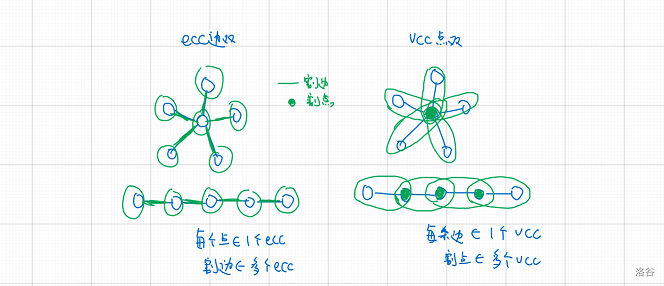
\includegraphics[width=10cm]{images/ecc.png}
\end{figure}
\par \noindent 在一个无向图中,若任意两点间至少存在两条 “点不重复” 的路径,则说这个图是点双连通的,在一个无向图中,点双连通的极大子图称为\textbf{点双连通分量} 。
~\\
\par \noindent 点双连通图定义等价于:任意两条边都在同一个简单环中。
~\\
\par \noindent 【点双联通分量vDCC】:分量中没有割点,每条边属于1个点双,割点属于多个点双。

\begin{minted}{c++}
namespace vDCC {
    int dfn[maxn], low[maxn], timestamp = 0, rt = 0, dcccnt = 0;
    bool cut[maxn];      // 记录点 i 是不是割点
    stack<int> stk;
    vector<int> dcc[maxn];
    void tarjan(int u, int fa) {
        dfn[u] = low[u] = ++timestamp;
        stk.push(u);
        if (u == rt && h[u] == -1) {       // 孤立点,单独成图 
            dcc[++dcccnt].push_back(u);
            return;
        }
        int child_count = 0;
        for (int i = h[u]; i != -1; i = ne[i]) {
            int v = e[i];
            if (!dfn[v]) {
                tarjan(v, u);
                low[u] = min(low[u], low[u]);
                child_count++;
                if (low[v] >= dfn[u]) {    // u是割点或根 
                    if (u != rt || child_count > 1) cut[u] = 1;
                    ++dcccnt;
                    int y;
                    do {
                        y = stk.top(), stk.pop();
                        dcc[dcccnt].push_back(y);
                    } while (y != v);
                    dcc[dcccnt].push_back(u);
                }
            } else if(v != fa)
                low[u] = min(low[u], dfn[v]);
        }
    }
    int solve(int n) {
        for (int i = 1; i <= n; i++)
            if (!dfn[i])
                rt = i, tarjan(i, 0);
        return dcccnt; // 返回点双连通分量个数 v-dcc
    }
    void add_vdcc_edge(int u, int v){}
    
    int num, new_id[maxn], c[maxn];
    void shrink() {
        num = dcccnt;
        // 给割点编号
        for (int i = 1; i <= n; i++)
            if (cut[i])
                new_id[i] = ++num;
        for (int i = 1; i <= dcccnt; i++) {
            for (int j = 0; j < (int)dcc[i].size(); j++) {
                int x = dcc[i][j];
                if (cut[x])
                    add_vdcc_edge(i, new_id[x]), add_vdcc_edge(new_id[x], i);
                else
                    c[x] = i;           // 除了割点之外,标记其它的点只属于一个 v-DCC
            }
        }
    }
}using namespace vDCC;
\end{minted}
\par \noindent 对每个点双,新建一个方点来表示。点双中所有圆点向这个方点连边,原无向图 $\to$ 一棵树
\par \noindent 
\begin{figure}[H]
        \centering
        \par 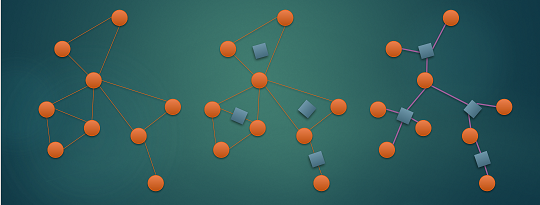
\includegraphics[width=10cm]{images/ecc-tree.png}
\end{figure}

\par \noindent 圆方树的性质:
\begin{enumerate}
\item 圆点方点相间
\item 在圆方树中,原来的每个点对应一个 \textbf{圆点},每一个点双对应一个 \textbf{方点}。
\item 对于每一个度数 $=1$ 的圆点,都对应唯一方点
\item 原图的割点是圆方树中度数 $>1$ 的圆点
\item 原图中每条边,都对应唯一方点 $x$
\item 无论取哪个点为根开始dfs建圆方树,圆方树的形态是一样的
\end{enumerate}
\begin{minted}{c++}
// 小粉图博客 圆方树构建过程
#include <cstdio>
#include <vector>
#include <algorithm>

const int MN = 100005;

int N, M, cnt;
std::vector<int> G[MN], T[MN * 2];

int dfn[MN], low[MN], dfc;
int stk[MN], tp;

void Tarjan(int u) {
    printf("  Enter : #%d\n", u);
    low[u] = dfn[u] = ++dfc; // low 初始化为当前节点 dfn
    stk[++tp] = u; // 加入栈中
    for (int v : G[u]) { // 遍历 u 的相邻节点
        if (!dfn[v]) { // 如果未访问过
            Tarjan(v); // 递归
            low[u] = std::min(low[u], low[v]); // 未访问的和 low 取 min
            if (low[v] == dfn[u]) { // 标志着找到一个以 u 为根的点双连通分量 试了试>= 同样正确
                ++cnt; // 增加方点个数
                printf("  Found a New BCC #%d.\n", cnt - N);
                // 将点双中除了 u 的点退栈,并在圆方树中连边
                for (int x = 0; x != v; --tp) {
                    x = stk[tp];
                    T[cnt].push_back(x);
                    T[x].push_back(cnt);
                    printf("    BCC #%d has vertex #%d\n", cnt - N, x);
                }
                // 注意 u 自身也要连边(但不退栈)
                T[cnt].push_back(u);
                T[u].push_back(cnt);
                printf("    BCC #%d has vertex #%d\n", cnt - N, u);
            }
        } else low[u] = std::min(low[u], dfn[v]); // 已访问的和 dfn 取 min
    }
    printf("  Exit : #%d : low = %d\n", u, low[u]);
    printf("  Stack:\n    ");
    for (int i = 1; i <= tp; ++i) printf("%d, ", stk[i]);
    puts("");
}

int main() {
    scanf("%d%d", &N, &M);
    cnt = N; // 点双 / 方点标号从 N 开始
    for (int i = 1; i <= M; ++i) {
        int u, v;
        scanf("%d%d", &u, &v);
        G[u].push_back(v); // 加双向边
        G[v].push_back(u);
    }
    // 处理非连通图
    for (int u = 1; u <= N; ++u)
        if (!dfn[u]) Tarjan(u), --tp;
        // 注意到退出 Tarjan 时栈中还有一个元素即根,将其退栈
    return 0;
}
\end{minted}

\subsection{求无向图边双连通分量 \& 缩点}
\par \noindent \textbf{边双连通} 如果任意两点至少存在两条边不重复路径,则称该图为边双连通的。
~\\
\par \noindent 【边双联通分量ecc】:分量中没有割边,每个点属于1个边双,割边属于多个边双。

\begin{minted}{c++}
namespace eDCC {
    int dfn[maxn], low[maxn], timestamp, dcnt = 0;
    int c[maxn]; // 缩点后的编号
    bool is_bridge[maxn];
    void tarjan(int u, int from) {
        dfn[u] = low[u] = ++timestamp;
        // stk.push(u);
        for (int i = h[u]; i != -1; i = ne[i]) {
            int v = e[i];
            if (!dfn[v]) {
                tarjan(v, i);
                low[u] = min(low[u], low[v]);
                if (low[v] > dfn[u]) is_bridge[i] = is_bridge[i^1] = 1;// 该边是桥
            }
            else if (i != (from ^ 1))
                low[u] = min(low[u], dfn[v]);
        }
        // 栈的方式缩点
        // if(dfn[u] == low[u]) {
        //     ++dcnt;
        //     int y;
        //     do{
        //         y = stk.top();stk.pop();
        //         c[y] = dcnt;
        //     }while(y != u);
        // }
    }
    // 先找出桥 然后dfs不走桥标记点 看出染色的过程
    void dfs(int u, int co) {
        c[u] = co;
        for (int i = h[u]; i != -1; i = ne[i]) {
            int v = e[i];
            // 节点 y 已被访问或者 (x,y) 是桥 
            if (c[v] || is_bridge[i])
                continue;
            dfs(v, co);
        }
    }
    void solve(int n) {
        for (int i = 1; i <= n; i++)
            if (!dfn[i])
                tarjan(i, 0);
        for (int i = 1; i <= n; i++)
            if (!c[i])
                dfs(i, ++dcnt);
    }

    void add_cut_edge(int u, int v) {}
    void shrink() {
        for (int i = 0; i < idx; i += 2) {     // idx 是前向星的个数
            int v = e[i], u = e[i^1];
            if (c[v] == c[u])
                continue;                   // x, y 同属一个 e-DCC, 无事可做
            add_cut_edge(c[u], c[v]);       // 否则将 x, y 加入新图中
        }
    }    
}using namespace eDCC;
\end{minted}
% 最近公共祖先
\section{最近公共祖先}
\par \noindent 树上多个点的LCA,就是DFS序最小的和DFS序最大的这两个点的LCA。
\subsection{倍增法求 LCA}
\begin{minted}{c++}
int lca(int a,int b)
{
    if(dep[a]<dep[b]) swap(a,b);
    for(int k=20;k>=0;k--)
        if(dep[fa[a][k]]>=dep[b]) a=fa[a][k];
    if(a==b) return a;
    for(int k=20;k>=0;k--)
        if(fa[a][k]!=fa[b][k]) a=fa[a][k],b=fa[b][k];
    return fa[a][0];
}
\end{minted}

\subsection{O(1)询问LCA}
\par \noindent 基于 SPFA 的负环判定,使用 inqcnt[v] 记录节点 v 的入队次数,如果有一个点的 inqcnt[v] > n,说明存在负环。

\par \noindent 或者记录最短路经过的边数,在不经过负环的情况下,最短路至多经过 n - 1 条边,因此如果经过了多于 n 条边,一定说明经过了负环
\begin{minted}{c++}
#include<bits/stdc++.h>

using namespace std;
const int N=1000010;

int h[N],e[N<<1],ne[N<<1],idx;
void add(int a,int b){e[idx]=b,ne[idx]=h[a],h[a]=idx++;}
int dfn[N],timstamp;
int n,m,rt;
int dep[N],rev[N],fa[N];
void dfs(int u)
{
    dep[u]=dep[fa[u]]+1;
    dfn[u]=++timstamp;
    rev[timstamp]=u;
    for(int i=h[u];i!=-1;i=ne[i])
    {
        int v=e[i];
        if(v==fa[u]) continue;
        fa[v]=u;
        dfs(v);
    }
}
int inline MIN(int x,int y){return dep[x]<dep[y]?x:y;}

int st[N][21];
int lg[N];
int lca(int u,int v)
{
    if(u==v) return u;
    u=dfn[u],v=dfn[v];
    if(u>v) swap(u,v);
    u++;
    int k=lg[v-u+1];
    return fa[MIN(st[u][k],st[v-(1<<k)+1][k])]; 
}
int main()
{
    ios::sync_with_stdio(false);cin.tie(nullptr);cout.tie(nullptr);
    cin>>n>>m>>rt;
    for(int i=1;i<=n;i++) h[i]=-1;
    for(int i=1;i<n;i++)
    {
        int a,b;cin>>a>>b;
        add(a,b),add(b,a);
    }
    dfs(rt);
    for(int i=2;i<=n;i++) lg[i]=lg[i>>1]+1;
    for(int i=1;i<=n;i++) st[i][0]=rev[i];
    for(int k=1;k<=lg[n];k++) 
        for(int i=1;i+(1<<k)-1<=n;i++) 
            st[i][k]=MIN(st[i][k-1],st[i+(1<<k-1)][k-1]);

    while(m--)
    {
        int x,y;cin>>x>>y;
        cout<<lca(x,y)<<'\n';
    }
    return 0;
}
\end{minted}

\subsection{【模板】树上 k 级祖先}
\par \noindent 长链剖分的经典应用。

\par \noindent 显然这个问题有 $\mathcal{O}(n \log n)-\mathcal{O}(\log n)$ 的树上倍增做法,然而还不够优秀。
~\\
\par \noindent 首先我们进行预处理:

\begin{enumerate}
\item 对树进行长链剖分,记录每个点所在链的顶点和深度, $\mathcal{O}(n)$ 。
\item 树上倍增求出每个点的 $2^n$ 级祖先, $\mathcal{O}(n \log n)$ 。
\item 对于每条链,如果其长度为 len,那么在顶点处记录顶点向上的 len 个祖先和向下的 len 个链上的儿 子, $\mathcal{O}(n)$ 。
\item 对 $i \in[1, n]$ 求出在二进制下的最高位 $h_i$,$\mathcal{O}(n)$ 。
   对于每次询问 $x$ 的 $k$ 级祖先:
\item 利用倍增数组先将 $x$ 跳到 $x$ 的 $2^{h_k}$ 级祖先,设剩下还有 $k^{\prime}$ 级,显然 $k^{\prime}<2^{h_k}$ ,因此此时 $x$ 所在的长 链长度一定 $\geq 2^{h_k}>k^{\prime}$ 。
\item 由于长链长度 $>k^{\prime}$ , 因此可以先将 $x$ 跳到 $x$ 所在链的顶点,若之后剩下的级数为正,则利用向上的数 组求出答案,否则利用向下的数组求出答案。
   这样时间复杂度为 $\mathcal{O}(n \log n)-\mathcal{O}(1)$ 的。
\end{enumerate}
\begin{minted}{c++}
#include<bits/stdc++.h>

using namespace std;
using ll = long long;


const int N = 5e5 + 7;
int n, q, rt, lg[N], d[N], fa[N][21], son[N], dep[N], top[N], ans;
vector<int> e[N], u[N], v[N];
unsigned int s;
ll Ans;

inline unsigned int get(unsigned int x) {
    return x ^= x << 13, x ^= x >> 17, x ^= x << 5, s = x; 
}

void dfs(int x) {
    // dep[x] x子树的最大深度
    // d[x] x的深度
    dep[x] = d[x] = d[fa[x][0]] + 1;
    for (auto y : e[x]) {
        fa[y][0] = x;
        for (int i = 0; fa[y][i]; i++) fa[y][i+1] = fa[fa[y][i]][i];
        dfs(y);
        if (dep[y] > dep[x]) dep[x] = dep[y], son[x] = y;
    }
}

void dfs(int x, int p) {
    top[x] = p; // 每个长链的顶点 dep[x] 若 x 是顶点 那么dep[x]-d[x]则是链的长度
    if (x == p) {
        for (int i = 0, o = x; i <= dep[x] - d[x]; i++)
            u[x].push_back(o), o = fa[o][0];
        for (int i = 0, o = x; i <= dep[x] - d[x]; i++)
            v[x].push_back(o), o = son[o];
    }
    if (son[x]) dfs(son[x], p);
    for (auto y : e[x]) if (y != son[x]) dfs(y, y);
}

inline int ask(int x, int k) {
    if (!k) return x;
    x = fa[x][lg[k]], k -= 1 << lg[k], k -= d[x] - d[top[x]], x = top[x];
    return k >= 0 ? u[x][k] : v[x][-k];
}

int main() {
    ios::sync_with_stdio(false);cin.tie(nullptr);cout.tie(nullptr);
    cin >> n >> q >> s;
    lg[0] = -1;
    for (int i = 1; i <= n; i++)
        cin>>fa[i][0], e[fa[i][0]].push_back(i), lg[i] = lg[i>>1] + 1;
    rt = e[0][0], dfs(rt), dfs(rt, rt);
    
    for (int i = 1, x, k; i <= q; i++) {
        x = (get(s) ^ ans) % n + 1;
        k = (get(s) ^ ans) % d[x];
        Ans ^= 1ll * i * (ans = ask(x, k));
    }
    cout << Ans << '\n';
    return 0;
}
\end{minted}
% 2-SAT问题
\section{2-SAT 问题}
\begin{tcolorbox}
\par \noindent \textbf{定义}:简单的说就是给出n个集合,每个集合有两个元素,已知若干个$<a,b>$,表示 $a$ 与 $b$ 矛盾(其中 $a$ 与 $b$ 属于不同的集合)。然后从每个集合选择一个元素,判断能否一共选n个两两不矛盾的元素。
\end{tcolorbox}
\par \noindent \textbf{原理}: 首先建图: 假设两个集合 $\left\{a_1, b_1\right\}$ 和 $\left\{a_2, b_2\right\}$, 如果 $a_1, b_2$ 冲突, 那么连有向边 $\left(a_1, b_1\right)$ 和 $\left(b_2, a_2\right)$, 然后跑一遍 Tarjan 有向图缩点, 判断是否有一个集合的两个元素同时在同一个 SCC 中, 如果有则无 解, 否则有解。
~\\
\par \noindent \textbf{输出方案}: Tarjan 算法求强连通分量时用了栈, 求得各点所在的 SCC 编号相当于反拓扑序。对于任 意集合可以表示为 $\{x, \neg x\}$; 如果变量 $\neg x$ 的拓扑序在 $x$ 之后(即 $\operatorname{topo}(\neg x) \geq \operatorname{topo}(x)$ ), 则取 $x$ 为真。
\begin{minted}{c++}
namespace TwoSAT {
    #define clear(x) memset(x, 0, sizeof(x))
    int head[maxn], dfn[maxn], low[maxn], c[maxn], stk[maxn];
    int top = 0, scccnt = 0, order = 1, cnt = 1;
    bool instack[maxn];
    struct Edge {
        int u, v, next;
        Edge(int u = 0, int v = 0, int next = 0): u(u), v(v), next(next) {}
    } e[maxm];
    void add_edge(int u, int v) {
        e[cnt] = Edge(u, v, head[u]);
        head[u] = cnt++;
    }
    void init() {
        clear(dfn), clear(low), clear(c), clear(instack), clear(head);
        scccnt = 0, order = 1, cnt = 1, top = 0;
    }
    void tarjan(int x) {
        dfn[x] = low[x] = order++;
        stk[++top] = x, instack[x] = 1;
        for (int i = head[x]; i; i = e[i].next) {
            int y = e[i].v;
            if (!dfn[y])
                tarjan(y), low[x] = min(low[x], low[y]);
            else if (instack[y])
                low[x] = min(low[x], dfn[y]);
        }
        if (dfn[x] == low[x]) {
            int tmp;
            do {
                tmp = stk[top--];
                c[tmp] = scccnt, instack[tmp] = 0;
            } while (tmp != x);
            scccnt++;
        }
    }
    void shrink(int n) {
        for (int x = 0; x <= n; x++)
            if (!dfn[x])
                tarjan(x);
    }
    bool solve(int n) {
        shrink(n);
        for (int i = 0; i <= n; i += 2)
            if (c[i] == c[i+1])
                return false;
        return true;
    }
}using namespace TwoSAT;
\end{minted}
% 差分约束
\section{差分约束}

\par \noindent 求解差分约束系统,有 $m$ 条约束条件,每条都为形如 $x_a-x_b\geq c_k$,$x_a-x_b\leq c_k$ 或 $x_a=x_b$ 的形式,判断该差分约束系统有没有解。
~\\
\par \noindent 
\par \noindent 跑判断负环,如果不存在负环,输出 `Yes`,否则输出 `No`。
~\\
\par \noindent 如果${x_1,x_2,...,x_n}$是该差分约束系统的一组解,那么对于任意常数 $d$, ${x_1+d,x_2+d,...,x_n+d}$显然也是该差分约束系统的一组解,因为这样做差后 $d$ 会被消掉。
~\\
\par \noindent \textbf{步骤:} 

\begin{enumerate}
\item 先将每个不等式$x_a - x_b \leq c$,转换成一条从 $x_b$ 走到 $x_a$,长度为 $c$ 的边。
\item 找到一个超级源点,使得该源点一定可以走到所以边
\item 从源点求一遍单源最短路
\end{enumerate}

\par \noindent \textbf{结果1:}如果存在负环,则原不等式组一定无解
\par \noindent \textbf{结果2:}如果没有负环,则 $dist[i]$ 就是原不等式组的一个可行解
~\\
\par \noindent \textbf{最大值和最小值结论:}

\begin{itemize}
\item 如果求的是最小值,则应该求最长路

\item 如果求的是最大值,则应该求最短路
\end{itemize}

\par \noindent 比如求\textbf{最小解},只需要求\textbf{最长路}就行了。最长路满足三角形不等式$dist[u]≥dist[v]+w_{v,u}$
% 虚数
\section{虚树}

\par \noindent 给定一棵树,有多次询问,每组询问对树上的一些关键点,询问它们的某些信息,满足所有询问中的关键点数量\textbf{总和}与树的大小同阶。此时可以对原树建立一棵只包含关键点和 LCA 的虚树,可以将问题的复杂度压缩到 $O(Q \log_2N + f(Q))$ 的等级。
~\\
\par \noindent \textbf{关键性质:}在一棵有根树中,任选 $k$ 个不重复的点,这  $k$ 个点两两之间的不同 LCA 数量不超过  $k-1$  个(即  $k$ 个点两两之间的 LCA 数量不超过自身的阶数)。
\begin{minted}{c++}
namespace VirtualTree {
    
    vector<int> VT[maxn];
    
    inline bool cmp(const int &i, const int &j) {
        return dfn[i] < dfn[j];
    }
    // 构建虚树
    void build_virtual_tree(int node[], int k) {
        static int stk[maxn];
        // k 个关键节点
        sort(node, node + k, cmp), top = 0;
        // stk[top = 1]  = 1; // 根节点入栈
        for (int i = 0; i < k; i++) {   
            if (i == 0)
                assert(node[i] == 1); // 根节点是关键节点
            if (top <= 1) {
                stk[++top] = node[i];
                continue;
            }
            int u = node[i], p = lca(u, stk[top]);
            if (p == stk[top]) {
                stk[++top] = u;
                continue;
            }
            while (top > 1 && dfn[p] <= dfn[stk[top-1]])
                VT[stk[top-1]].emplace_back(stk[top]), top--;
            if (p != stk[top])
                VT[p].emplace_back(stk[top]), stk[top] = p;
            stk[++top] = u;
        }
        for (int i = 1; i < top; i++)
            VT[stk[i]].emplace_back(stk[i+1]);
    }

    void calc_vt_depth(int x, int p) {
        fa[x] = p, vdepth[x] = vdepth[p] + 1;
        for (int i : VT[x])
            calc_vt_depth(i, x);
    }
    // void clear()  构建的时候清空 或者dfs过程遍历完就清空
}using namespace VirtualTree;

// 处理路径 (u, v) 上的更新和询问 
ll a[maxn], w[maxn];
// 更新
while (u != v) {
    if (rdp[u] < rdp[v])
        swap(u, v);
    w[u] += x, a[u] += x, u = fa[u];
}
a[u] += x;
// 询问
ll ans = 0;
while (u != v)  {
    if (rdp[u] < rdp[v])
        swap(u, v);
    if (depth[u] - depth[fa[u]] - 1)
        ans += w[u] * (depth[u] - depth[fa[u]] - 1);    // 用 depth 统计 
    ans += a[u];
}
ans += a[u];
\end{minted}
%
%% Chapter 3 网络流/二分图/匹配
\chapter{网络流/二分图/匹配}

% 二分图匹配
\section{二分图}
\subsection{匈牙利算法}
\par \noindent 考虑点集A,B二分图
\par \noindent \textbf{最小点覆盖}:
\par \noindent 概念:用最少的点覆盖二分图中所有边。
\par \noindent 结论:最小覆盖点=最大匹配
\par \noindent 
\par \noindent \textbf{最小边覆盖}:
\par \noindent 概念:用最少的边覆盖点集A,B中的所有点。
\par \noindent 结论:最小边覆盖=总点数-最大匹配
\par \noindent 
\par \noindent \textbf{最大独立集}
\par \noindent 概念:选出最多的点使得点集内部没有边。
\par \noindent 结论:最大独立集=总点数-最大匹配
\par \noindent 
\par \noindent \textbf{最小路径点覆盖}
\par \noindent 概念:对于一个有向图,选出最少的不相交路径使其覆盖所有点。
\par \noindent 结论:最小路径覆盖=总点数-最大匹配
\par \noindent 
\par \noindent \textbf{最小路径重复点覆盖}
\par \noindent 概念:对于一个有向图,选出最少的(能相交)路径使其覆盖所有点。
\par \noindent 结论:对原图求传递闭包之后再对新图求最小不相交路径覆盖

\begin{minted}{c++}
int match[manx], vis[manx];
bool dfs(int x) {
// 遍历 x 的每条出边
    for (int i = h[x], y; i != -1; i = ne[i]) {
        y = e[i];
        // 如果在当前递归 DFS 的过程中,y 没有被访问过
        if (!vis[y]) {
            vis[y] = 1; // 先将 y 分配给 x, 标记 y 被访问
        // 如果 y 没有被匹配,那就让它与 x 匹配
        // 否则,尝试对 y 已匹配的边匹配其他的节点,然后再让 y 与 x 匹配
        if (!match[y] || dfs(match[y])) {
                match[y] = x;
                return true;
            }
        }
    }
    // 如果走到了这里,说明该点匹配失败
    return false;
}
int main() {
    int ans = 0;
    for (int i = 1; i <= n; i++) {
    // 重设 vis 数组,表示所有点都不在增广路中
        memset(vis, 0, sizeof vis);
    // 尝试为每个点匹配(找增广路),如果匹配成功则 ans++
    if (dfs(i)) ans++;
    }
}
\end{minted}

\subsection{KM算法}
\par \noindent 解决二分图最大带权匹配,时间复杂度 $O(n^3)$.
\begin{minted}{c++}
#include<cstdio>
#include<cstring>
#include<iostream>
#include<algorithm>
using namespace std;
typedef long long ll;
const int N=510;
ll w[N][N],lx[N],ly[N];//顶标
bool visx[N],visy[N];//记录是否在交错树上
int match[N];//匹配
int n,m,p[N];
ll delta,c[N];//delta和更新后的delta
void bfs(int x)
{
    int a,y=0,y1=0;
    for(int i=1;i<=n;i++) p[i]=0,c[i]=1e18;
    match[y]=x;
    do{
        a=match[y],delta=1e18,visy[y]=1;
        for(int b=1;b<=n;b++)
            if(!visy[b])
            {
                if(c[b]>lx[a]+ly[b]-w[a][b])
                    c[b]=lx[a]+ly[b]-w[a][b],p[b]=y;
                if(c[b]<delta)//Δ还是取最小的
                    delta=c[b],y1=b;
            }
        for(int b=0;b<=n;b++)
            if(visy[b])
                lx[match[b]]-=delta,ly[b]+=delta;
            else
                c[b]-=delta;
        y=y1;
    }while(match[y]);
    while(y) match[y]=match[p[y]],y=p[y];
}
ll KM()
{
    for(int i=1;i<=n;i++)
        match[i]=lx[i]=ly[i]=0;
    for(int i=1;i<=n;i++)
    {
        memset(visy,0,sizeof visy);
        bfs(i);
    }
    
    ll res=0;
    for(int i=1;i<=n;i++)
        res+=w[match[i]][i];
    return res;
}
int main()
{
    scanf("%d%d",&n,&m);
    for(int i=1;i<=n;i++)
        for(int j=1;j<=n;j++) 
            w[i][j]=-1e18;
    for(int i=1;i<=m;i++)
    {
        int a,b;ll c;
        scanf("%d%d%lld",&a,&b,&c);
        w[a][b]=max(w[a][b],c);
    }
    printf("%lld\n",KM());
    for(int i=1;i<=n;i++)
        printf("%d ",match[i]);
    puts("");
    return 0;
}
\end{minted}

\subsection{染色判二分图}
\begin{minted}{c++}
int vis[MAXN], flag = 1;
void dfs(int x, int co) {
    vis[x] = co;
    for (int i = h[x]; i != -1; i = ne[i]) {
        if (vis[e[i]] == 0)
            dfs(vis[e[i]], 3 - co); // 注意这里的小技巧,3-1=2, 3-2=1.
        else if (vis[e[i]] == co) {
            flag = 0;
            return;
        }
    }
}
for (int i = 0; i < n; i++) {
    if (!vis[i] && flag)
        dfs(i, 1);
    if (!flag) break;
}
printf(flag ? "Yes" : "No");
\end{minted}
\clearpage

% 最大流
\section{最大流}

\subsection{Dinic 算法 (带当前弧优化)}

\par 不断在残量图上使用 BFS 求出结点的层次,构建分层图(即给结点标注 d[i]);然后在分层图上 DFS 寻找增广路,回溯时实时更新剩余容量。每个点可以流向多条出边。时间复杂度为 $O(n^2m)$。
\begin{minted}{c++}
template <int N> struct Dinic {
    const int INF = 1e9;
    struct E {
        int to, cap, rev;// x->y 目标点 to=y 流量cap 反向边G[to][rev]=x
    };
    vector<E> G[N];
    int lev[N], cur[N];// 层数 当前弧优化
    inline void add(int x, int y, int c) {
        G[x].push_back({ y, c, (int)G[y].size() });
        G[y].push_back({ x, 0, (int)G[x].size() - 1 });
    }
    void bfs(int s) {
        queue<int> q;
        memset(lev, -1, sizeof lev);

        for (lev[s] = 0, q.push(s); q.size();) {
            int x = q.front();
            q.pop();

            for (auto &e : G[x])
                if (e.cap > 0 && lev[e.to] < 0)// 层数未赋值 容量大于0
                    lev[e.to] = lev[x] + 1, q.push(e.to);
        }
    }
    int dfs(int x, int t, int f) {
        if (x == t)
            return f;
        // 当前弧优化
        for (int &i = cur[x], sz = G[x].size(), d; i < sz; i++) {
            auto &e = G[x][i];

            if (e.cap > 0 && lev[x] < lev[e.to]) {// lev[e.to]==lev[x]+1
                if ((d = dfs(e.to, t, min(f, e.cap))) > 0) {
                    e.cap -= d, G[e.to][e.rev].cap += d;// 正向边流量-d 反向边容量+d
                    return d;
                }
            }
        }

        return 0;
    }
    int64_t maxflow(int s, int t) {
        for (int64_t flow = 0, f;;) {
            bfs(s);

            if (lev[t] < 0)// BFS未遍历到终点
                return flow;

            memset(cur, 0, sizeof cur);// 当前弧指向第一条边即G[x][0]

            while ((f = dfs(s, t, INF)) > 0)
                flow += f;
        }
    }
};
Dinic<10010> din;
\end{minted}

\subsection{无源汇上下界可行流}
\par \textbf{问题:} 给定一个网络,求一个流满足:每条边的流量处在给定的下界和上界 [lower,upper] 之间,满足流量守恒

\begin{itemize}
\item 记$A(u)=\sum_{to [i]=u}f(i)-\sum_{from[i]=u}f(i)$即流入减去流出
\item 若$A(u)>0$,源点 $S$ 向 $u$ 点连边,容量是$A(u)$
\item 若$A(u)<0$,$u$ 点向汇点 $T$ 连边,容量是$-A(u)$
\end{itemize}
如果\textbf{满流}(虚拟源点 S 流跑满)此时即可求出流2(否则无解),再加上流1即是满足题意的可行流
\begin{minted}{c++}
int main() {

    cin >> n >> m;
    S = 0, T = n + 1; // 虚拟源点 汇点
    for (int i = 1; i <= m; i++) {
        int x, y, c, d; cin >> x >> y >> c >> d;
        din.add(x, y, d - c, i);
        in[y] += c, out[x] += c;
        l[i] = c;
    }
    int sum = 0;
    for (int i = 1; i <= n; i++) {
        if (in[i] > out[i])
            din.add(S, i, in[i] - out[i], 0), sum += in[i] - out[i]; // 满流
        else
            din.add(i, T, out[i] - in[i], 0);
    }
    if (sum != din.maxflow(S, T))
        cout << "NO\n";
    else {
        cout << "YES\n";
        for (int x = 1; x <= n; x++)
            for (auto [y, cap, rev, id] : din.G[x]) {
                ans[id] = cap;
            }
        for (int i = 1; i <= m; i++)
            cout << ans[i] + l[i] << '\n';
    }
    return 0;
}
\end{minted}
\subsection{有源汇上下界最大流}
\par \noindent 连接一条 $t\to s$下界是 0 上界是 $\infty$ 的边,由此转化循环流问题(无源汇上下界可行流)
\par \noindent 
\par \noindent 按照循环流问题建图,首先跑 $S \to T$ 的dinic 是否能够找到一条可行流(即判断是否是满流)然后在换源点和汇点并删去 $t\to s$ 的边再跑一边 $s\to t$ dinic(榨干残留网络),可行流 + 第二次dinic即是最大流
\begin{minted}{c++}
int main() {

    // ............. 无源汇上下界可行流建图
    din.add(t, s, 1e9);

    res = din.maxflow(S, T);

    if (res != sum) {
        cout << "No Solution\n";
        return 0;
    }
    auto &[v, cap, inv] = din.G[s].back();
    res = cap;
    din.erase(din.G[v][inv]); //删去 t->s 容量是1e9这条边
    cout << res + din.maxflow(s, t);
    return 0;
}
\end{minted}

\subsection{有源汇上下界最小流}
\par \noindent 最小流 = 可行流 + $s\to t$ 流,由于可行流固定,为了使结果最小即 $s\to t$ 流最小,由于 $s\to t$ 的流 = $- t\to s$的流,如果 $t\to s$ 求最大流,那么 $s\to t$ 就是最小流,$f_{s\to t}=-f_{t\to s}$ 这也是为什么相减的原因。
\begin{minted}{c++}
int main() {
    
    // ............. 无源汇上下界可行流建图
    din.add(t, s, 1e9);

    res = din.maxflow(S, T);

    if (res != sum) {
        cout << "No Solution\n";
        return 0;
    }

    auto &[v, cap, inv] = din.G[s].back();
    res = cap;
    din.erase(din.G[v][inv]); //删去 t->s 容量是1e9这条边

    cout << res - din.maxflow(t, s); // f(s->t) = - f(t->s)
    return 0;
}
\end{minted}


% 最小费用最大流
\section{最小费用最大流}
\subsection{Primal-Dual 原始对偶算法}
\par 给定一个网络 $G=(V, E)$,每条边 $(u, v) \in E$ 带有属性 $c(u, v)$,表示从当前边流过 1 个单位流量时的费用。在最大化流量的基础上,求最小的费用。

\begin{minted}{c++}
#include <bits/stdc++.h>
#define int long long
#pragma GCC optimize(2)
using namespace std;
const int inf=1e9;
template <int N> struct MCMF {
    struct E {
        int to, cap, val, inv;
    };
    vector <E> G[N];
    int lev[N], cur[N], h[N], pre[N], preu[N];
    void add(int u, int v, int f, int w) {
        G[u].push_back({v, f, w, (int)G[v].size()});
        G[v].push_back({u, 0, -w, (int)G[u].size() - 1});
    }
    void dijkstra(int st) {
        priority_queue<pair<int, int>, vector<pair<int, int>>, greater<pair<int, int>>>q;
        memset(lev, 0x3f, sizeof lev);
        memset(pre, -1, sizeof pre);
        memset(preu, -1, sizeof preu);
        lev[st] = 0;
        q.push({0, st});

        while (q.size()) {
            auto [d, u] = q.top();
            q.pop();

            if (lev[u] < d) continue;

            int x = 0;

            for (auto [v, f, w, inv] : G[u]) {
                if (f && lev[v] > lev[u] + w + h[u] - h[v]) {
                    lev[v] = lev[u] + h[u] - h[v] + w;
                    pre[v] = x;
                    preu[v] = u;
                    q.push({lev[v], v});
                }
                x++;
            }
        }
    }
    pair<int, int> min_cost_max_flow(int st, int ed) {
        memset(h, 0, sizeof h);

        for (int flow = 0, cost = 0, res = inf;; res = inf) {

            dijkstra(st);

            if (lev[ed] > inf)
                return {flow, cost};

            for (int i = 0; i < N; i++) {
                h[i] += lev[i];
            }

            for (int i = ed; i != st; i = preu[i]) {
                res = min(res, G[preu[i]][pre[i]].cap);
            }

            flow += res;
            cost += res * h[ed];

            for (int i = ed; i != st; i = preu[i]) {
                G[i][G[preu[i]][pre[i]].inv].cap += res;
                G[preu[i]][pre[i]].cap -= res;
            }
        }
    }
};

MCMF<5005>mcmf;
int n, m, s, t;

signed main() {
    ios::sync_with_stdio(false);
    cin.tie(0);
    cout.tie(0);
    cin >> n >> m >> s >> t;

    for (int i = 1; i <= m; i++) {
        int u, v, w, c;
        cin >> u >> v >> w >> c;
        mcmf.add(u, v, w, c);
    }

    auto [f, c] = mcmf.min_cost_max_flow(s, t);
    cout << f << " " << c << '\n';
}
\end{minted}

\subsection{EK算法求最大流}

\begin{minted}{c++}
#include <queue>
#include <iostream>
#include <cstring>
#include <algorithm>
using namespace std;
const int N = 5010, M = 100010;
int h[N], e[M], ne[M], f[M], w[M], idx;
int d[N], flow[N], pre[N];
bool st[N];
queue<int> q;

void add(int a, int b, int c, int d) {
    e[idx] = b, f[idx] = c, w[idx] = d, ne[idx] = h[a], h[a] = idx++;
    e[idx] = a, f[idx] = 0, w[idx] = -d, ne[idx] = h[b], h[b] = idx++;
}
bool spfa(int s, int t) {
    memset(d, 0x3f, sizeof d);
    memset(flow, 0, sizeof flow);
    d[s] = 0, flow[s] = 0x3f3f3f3f;
    q.push(s);

    while (q.size()) {
        int u = q.front();
        q.pop();
        st[u] = 0;

        for (int i = h[u]; i != -1; i = ne[i]) {
            int v = e[i];

            if (f[i] && d[v] > d[u] + w[i]) {
                d[v] = d[u] + w[i];
                pre[v] = i;
                flow[v] = min(f[i], flow[u]);

                if (!st[v]) {
                    q.push(v);
                    st[v] = 1;
                }
            }
        }
    }

    return flow[t] > 0;
}
pair<int, int> EK(int s, int t) {
    int maxflow = 0, mincost = 0;

    while (spfa(s, t)) {
        int r = flow[t];
        maxflow += r, mincost += r * d[t];

        for (int i = t; i != s; i = e[pre[i] ^ 1]) {
            f[pre[i]] -= r;
            f[pre[i] ^ 1] += r;
        }
    }

    return make_pair(maxflow, mincost);
}
int n, m, s, t;
int main() {
    cin >> n >> m >> s >> t;
    memset(h, -1, sizeof h);

    while (m--) {
        int a, b, c, d;
        cin >> a >> b >> c >> d;
        add(a, b, c, d);
    }

    auto [maxflow, mincost] = EK(s, t);

    cout << maxflow << ' ' << mincost << '\n';
    return 0;
}
\end{minted}

%
%% Chapter 4 字符串
\chapter{字符串和回文算法}

% Trie 树
\section{字典树}
\subsection{普通Trie}
\begin{minted}{c++}
struct Trie {
    int ch[maxn][30];
    bool has[maxn], vis[maxn];
    int cnt;
    void init() {
        memset(ch, 0, sizeof ch);
        memset(has, 0, sizeof has);
        memset(vis, 0, sizeof vis);
        cnt = 1;
    }
    void insert(char *s, int n) {
        int u = 0;
        for (int i = 0; s[i]; i++) {
            int c = s[i] - 'a';
            if (!ch[u][c]) ch[u][c] = ++cnt;
            u = ch[u][c];
        }
        has[u] = 1;
    }
    int query(char *s, int n) {
        int u = 0;
        for (int i = 0; i < n; i++) {
            int c = s[i] - 'a';
            if (!ch[u][c]) return -1;
            u = ch[u][c];
        }
        if (!has[u]) return -1;
        if (!vis[u]) {
            vis[u] = 1;
            return 0;
        } else
            return 1;
    }
};
\end{minted}
对于 0-1 字典树:
\begin{itemize}
\item 找异或最大值:当前位是 1 就走 0,是 0 就走 1,;走不通再走另一个;
\item 找与/或的最大值:以与运算为例,如果当前位是 1,那么肯定优先走 1;如果当前位是 0,那么当前位 和 0 或 1 运算的结果都是 0,我们无法确定走哪条支路才是最优解。于是我们可以将两条路合并成一条,把 1 的树自底向上合并到 0 的树
\end{itemize}

\subsection{压位Trie}
\begin{minted}{c++}
namespace BITWISE{
    inline int clz(unsigned long long x){return __builtin_clzll(x);}//这个函数是查询开头几个零
    inline int ctz(unsigned long long x){return __builtin_ctzll(x);}//这个函数是查询末尾几个零
} // namespace BITWISE

using namespace BITWISE;

typedef unsigned long long ull;
const int g = 6;
const int mod = (1 << g) - 1;
ull BUFF[1 << 25], *BT = BUFF + sizeof(BUFF) / sizeof(ull);//预先开好内存池
inline ull *alloc(int sz){return BT -= sz;}//动态分配空间
struct Trie{
    int dep;ull *a[5];//动态数组
    Trie(int sz){//初始化
        dep = 1;
        for(;;++ dep){
            int cnt = (sz + (1ull << g * dep) - 1) >> g * dep;//表示这一层有多少个点
            a[dep - 1] = alloc(cnt);
            if(cnt == 1) return ;
        }
        //注意这里层数越小越深,这样方便我们位运算
    }
    inline void ins(int x){
        for (int i = 0;i < dep;++ i){//自下而上遍历的
            ull p = 1ull << (x >> i * g & mod); //判断我们这个 x 在当前这一层要走哪一条边,并且直接左移好方便压位的处理
            if(a[i][x >> (i + 1) * g] & p) return ;//剪枝,上面有就可以弹出了
            a[i][x >> (i + 1) * g] |= p;
        }
    }
    inline void del(int x){
        for (int i = 0;i < dep;++ i)
            if(a[i][x >> (i + 1) * g] &= ~(1ull << (x >> i * g & mod))) return ;//删除一个位置,同样是删完还有就不删了的剪枝
    }
    inline int succ(int x){
        for (int i = 0;i < dep;++ i){
            int cur = (x >> i * g) & mod;ull v = a[i][x >> (i + 1) * g];//当前是哪一条边,由于这里只需要知道是哪一条边所以我们不需要左移
            if(v >> cur > 1){//如果存在前驱,也可以写成 v >> (cur + 1),后者更好理解但前者似乎更快
                int res = x >> (i + 1) * g << (i + 1) * g;
                res += (ctz(v >> (cur + 1)) + cur + 1) << i * g;//先把这一层的贡献加上,注意是不完整的
                for (int j = i - 1;~j;-- j) res += ctz(a[j][res >> (j + 1) * g]) << j * g;//剩下每一层都是完整的
                return res;//直接返回
            }
        }
        return 0;//否则返回零
    }
    inline int pre(int x){//与上面同理,不赘述
        for (int i = 0;i < dep;++ i){
            int cur = (x >> i * g) & mod;ull v = a[i][x >> (i + 1) * g];
            if(v & ((1ull << cur) - 1)){
                int res = x >> (i + 1) * g << (i + 1) * g;
                res += (mod - clz(v & ((1ull << cur) - 1))) << i * g;
                for (int j = i - 1;~j;-- j) res += (mod - clz(a[j][res >> (j + 1) * g])) << j * g;
                return res;
            }
        }
        return 0;
    }

};
Trie s(1 << 30);

void work(){
    /**
    1.插入 x 数(若已有 x 则不进行此操作);
    2.删除 x 数(若 x 不存在则不进行此操作);
    3.求 x 的前趋(前趋定义为 小于 x,且最大的数,若不存在则答案为 0);
    4.求 x 的后继(后继定义为 大于 x,且最小的数,若不存在则答案为 0);
    **/
    int op, x, ans;

      if(op == 0) s.ins(x);
    else if(op == 1) s.del(x);
    else if(op == 2) ans = s.pre(x);
    else ans = s.succ(x);
}
\end{minted}

% Hash
\section{Hash}
\subsection{字符串哈希}
\begin{minted}{c++}
#include<bits/stdc++.h>

using namespace std;
typedef unsigned long long ll;

const int N=1e5+5;

struct Hash {
    const int base = 131;           // 13331 19260817 防止哈希冲突
    const ll p = 212370440130137957;// (1ull<<61)-1 {402653189,805306457,1610612741,998244353}
 // 模两个质数的双哈希,建议取一些比较不常见的质数,比如 122420729,163227661,217636919, 1222827239, 998244353 等
    ll Pow[N], h[N];
 
    inline ll mul(ll x, ll y) {
        return (x * y - (ll) ((long double) x / p * y) * p + p) % p;
    }
    inline ll add(ll x, ll y) { return (x += y) >= p ? x - p : x; } 
 
    void init(char *s) {
        int l = strlen(s + 1); 
        Pow[0] = 1; 
        for (int i = 1; i <= l; ++i) Pow[i] = mul(Pow[i - 1], base);
        for (int i = 1; i <= l; ++i) h[i] = add(s[i], mul(h[i - 1], base));
    }
    ll get(int l, int r) { return add(h[r], p - mul(h[l - 1], Pow[r - l + 1])); }
} h;
//=======================双哈希
const basePrime1 = 233;
const basePrime2 = 13331;
// 模两个质数的双哈希,建议取一些比较不常见的质数,比如 122420729,163227661,217636919, 1222827239, 998244353 等
pair<int, int> double_hash(char *s, int n, int mod1, int mod2) {
    int hash1 = 0, hash2 = 0;
    for (int i = 0; i < n; i++)
        hash1 = (1LL * hash * basePrime1 + s[i]) % mod1,
        hash2 = (1LL * hash * basePrime2 + s[i]) % mod2;
    return make_pair(hash1, hash2);
}
\end{minted}
\subsection{手写Hash + 集合 Set(Set自带Hash)}

\par \noindent 拉链法也称开散列法(open hashing)。
~\\
\par \noindent 拉链法是在每个存放数据的地方开一个链表,如果有多个键值索引到同一个地方,只用把他们都放到那个位置的链表里就行了。查询的时候需要把对应位置的链表整个扫一遍,对其中的每个数据比较其键值与查询的键值是否一致。
\begin{tcolorbox}
\par \noindent 2020 CCPC秦皇岛 J. Jewel Splitting:https://codeforces.com/gym/102769/problem/J(哈希的各种技巧)
\end{tcolorbox}
\begin{minted}{c++}
#include<bits/stdc++.h>

using namespace std;
const int maxn = 310000;

const unsigned long long x = 23333;//131;
const long long mod = 998244353;
unsigned long long H[maxn], xp[maxn];
long long fac[maxn], inv[maxn];
char s[maxn];
int n;
void init() {
    n = strlen(s);
    H[n] = 0;
    for (int i = n - 1; i >= 0; --i)
        H[i] = H[i + 1] * x + s[i];// - 'a' + 1;
    xp[0] = 1;
    for (int i = 1; i <= n; ++i)
        xp[i] = xp[i - 1] * x;
}

inline unsigned long long Hash(int i, int d) {
    return H[i] - H[i + d] * xp[d];
}

//key_t应当为整数类型,且实际值必须非负
template<typename key_t, typename type> struct hash_table {
    static const int maxn = 610000;        // 哈希表的大小
    static const int table_size = 800;    // 索引的范围
    int first[table_size], nxt[maxn], sz; // init: memset(first, 0, sizeof(first)), sz = 0
    key_t id[maxn];
    type data[maxn];
    hash_table() {
        init();
    }
    void init(){
        memset(first, 0, sizeof(first));
        sz = 0;
    }
    type& operator[] (key_t key) {
        const int h = key % table_size;
        for (int i = first[h]; i; i = nxt[i])
            if (id[i] == key)
                return data[i];
        int pos = ++sz;
        nxt[pos] = first[h];
        first[h] = pos;
        id[pos] = key;
        return data[pos] = type();
    }
    bool count(key_t key) {
        for (int i = first[key % table_size]; i; i = nxt[i])
            if (id[i] == key)
                return true;
        return false;
    }
    type get(key_t key) { //如果key对应的值不存在,则返回type()。
        for (int i = first[key % table_size]; i; i = nxt[i])
            if (id[i] == key)
                return data[i];
        return type();
    }
};

struct Set {
    hash_table<unsigned long long, int> d;
    // 这个集合的 Hash
    unsigned long long code = 0;
    long long result = 1;// 题目需要
    void init() {
        code = 0;
        result = 1;
        d.init();
    }
    void insert(unsigned long long x) {
        auto val = d[x];
        d[x] += 1;
        result = result * fac[val] % mod * inv[val + 1] % mod; 
        unsigned long long t = val + 37;
        code += x * x * x + 7 * x * x + 3 * x + 7;
    }
    void erase(unsigned long long x) {
        auto val = d[x];
        d[x] -= 1;
        result = result * fac[val] % mod * inv[val - 1] % mod;
        unsigned long long t = val + 37;
        code -= x * x * x + 7 * x * x + 3 * x + 7;
    }
    auto hash() {
        return code;
    }
};
int main() {
    
    fac[0]= inv[1] = 1;
    for (int i = 1; i < maxn; ++i) fac[i] = fac[i - 1] * i % mod;
    for (int i = 2; i < maxn; i++) inv[i] = (long long)inv[mod % i] * (mod - mod / i) % mod;
    
    int T, kase = 0;
    scanf("%d", &T);
    Set S;
    hash_table<unsigned long long, int> vis;
    while (T--) {
        scanf("%s", s);
        init();
        long long ans = 0;
        for (int d = 1; d <= n; d++) {
            S.init();
            vis.init();
            for (int i = 0; i + d <= n; i += d) S.insert(Hash(i, d)); // hash [i, i + d)
            vis[S.hash()]++;
            
            ans += fac[n / d] * S.result % mod;
            int dis = n % d;
            if (dis == 0) continue;
            
            for (int i = n - dis - d; i >= 0; i -= d) {
                S.erase(Hash(i, d));
                S.insert(Hash(i + dis, d));
                if (!vis.count(S.hash())) {
                    vis[S.hash()]++;
                    ans += fac[n / d] * S.result % mod;
                }
            }
        }
        ans %= mod;
        printf("Case #%d: %lld\n", ++kase, ans);
    }
    return 0;
}
\end{minted}
\subsection{树Hash}
\begin{tcolorbox}
\par \noindent 给定一棵以点 1 为根的树,你需要输出这棵树中最多能选出多少个互不同构的子树。
~\\
\par \noindent 两棵有根树 T1、T2 同构当且仅当他们的大小相等,且存在一个顶点排列 σ 使得在 T1 中 $i$ 是 $j$ 的祖先当且仅当在 T2 中 $σ(i)$ 是 $σ(j)$ 的祖先。
\end{tcolorbox}
\begin{minted}{c++}
#include <bits/stdc++.h>
using namespace std;

typedef unsigned long long ull;

mt19937_64 rnd(chrono::steady_clock::now().time_since_epoch().count());
ull base = rnd();
const int N = 1e6 + 5;
int n, tot, sz[N];
ull h[N];
vector<int> e[N];

ull H(ull x) {
    return x * x * x * 11451419 + 19260817;
}
ull F(ull x) {
    return
        H(x & ((1ll << 32) - 1)) +
        H(x >> 32);
}
// 注释一种双Hash,需要预处理质数
void dfs(int u, int fa) {
    h[u] = base;
    // f1[u] = 1;
    // f2[u] = 0;
    for (int v : e[u]) {
        if (v == fa) continue;
        dfs(v, u);
        h[u] += F(h[v]);
        // f1[u] += f1[v] * prime[sz[v]];
        // f2[u] += f2[v] * base + sz[v];
    }
    // if (sz[u] == 1) f2[u] = 1;
}
int main() {
    scanf("%d", &n);
    for (int i = 1, u, v; i < n; ++i) {
        scanf("%d%d", &u, &v);
        e[u].push_back(v);
        e[v].push_back(u);
    }
    dfs(1, 0);
    sort(h + 1, h + 1 + n);
    printf("%d\n", unique(h + 1, h + 1 + n) - h - 1);
    return 0;
}
\end{minted}

% KMP
\section{KMP 算法}
\par \noindent 字符串 $s$ 的\textbf{border}:若 $s$ 的一个子串既是它的前缀又是它的后缀,则这个子串是它的border(一般不包含本身)
~\\
\par \noindent 字符串 $s$ 的\textbf{period}:循环节。用前 $T$ 个字符向后不断复制,能得到 $s$,最后一次可以只复制一部分

\begin{itemize}
\item \textbf{引理1}:如果有一个border $k$ 长度大于 $s$ 的一半,可以得出得 $s$ 有周期 $|s|−|k|$
\item \textbf{引理2}:如果 $p,q$ 都为周期,则 $\gcd(p,q)$ 也为周期
\item \textbf{引理3}:字符串 $s$ 所有不小于 $|s|$ 一半的border构成一个等差数列
\item \textbf{引理4}:可以把字符串分成 $log|s|$ 段,每一段的border都是一个等差数列
\end{itemize}

\begin{minted}{c++}
#include<iostream>
using namespace std;
const int N=1000010;
int n,m;
char p[N],s[N];
int ne[N];
int main()
{
    cin>>n>>p+1>>m>>s+1;
    // 求ne过程看成两个相同的串匹配
    for(int i=2,j=0;i<=n;i++)
    {
        while(j&&p[i]!=p[j+1]) j=ne[j];
        if(p[i]==p[j+1]) j++;// i结尾能够匹配 1~j 那么ne[i]=j
        ne[i]=j;
    }
    // 当前需要判断是否匹配 p[j+1]?=s[i]
    for(int i=1,j=0;i<=m;i++)
    {
        while(j&&s[i]!=p[j+1]) j=ne[j];
        if(s[i]==p[j+1]) j++;
        if(j==n)
        {
            cout<<i-n<<' ';
            j=ne[j];
        }
    }
    return 0;
}
\end{minted}

\subsection{Border等差数列}
\par \noindent 一个字符串的所有border可以被我们分成log数量级个等差数列。
~\\
\par \noindent 在 KMP 匹配中,我们可以利用这个性质快速跳过一串border
~\\
\par \noindent 具体而言,在一次跳border时,如果发现border长度不小于原串的一半,则接下来的border构成等差数列,直到一半以下(引理3),可以直接跳到 $(x−\lfloor\frac{\lfloor\frac{x}{2}\rfloor}{d}\rfloor×d)$。(网上博客直接跳到了 $x\mod d+d$处,经过几道题检验也是对的,但不是很能理解)
~\\
\par \noindent 一次至少跳一半,保证 $\log$ 次以内可以跳完
~\\
\begin{tcolorbox}
\par 有 $m$ 组询问,每组询问给定 $p, q$,求 $s$ 的 $p$ 前缀和 $q$ 前缀 的 \textbf{最长公共border} 的长度。
\end{tcolorbox}
\begin{minted}{c++}
#include <bits/stdc++.h>

using namespace std;
const int N = 1000010;
int n, m;
char s[N];int ne[N];
int main() {
    cin >> s + 1; n = strlen(s + 1);
    for (int i = 2, j = 0; i <= n; i++) {
        while (j && s[i] != s[j + 1]) j = ne[j];
        if (s[i] == s[j + 1]) j++;
        ne[i] = j;
    }
    int m; cin >> m;
    while (m--) {
        int p, q;
        cin >> p >> q;
        p = ne[p], q = ne[q];
        while (p != q) {
            if (p < q) swap(p, q);

            if (ne[p] > p / 2) {
                int d = p - ne[p];
                if (p % d == q % d)
                    p = q;
                else
                    p = p % d + d;
            } else
                p = ne[p];
        }
        cout << p << '\n';
    }
    return 0;
}
\end{minted}
\subsection{最小重复字符矩阵}

\begin{tcolorbox}
\par $q$ 组询问,每次询问一个矩形的最小重复字符矩阵,行列hash,为了在KMP加速匹配过程
\end{tcolorbox}
\begin{minted}{c++}
#include <iostream>
using namespace std;
typedef unsigned long long ull;
const int N = 2010;

const ull P = 13331;
int n, q;
char s[N][N];
ull hr[N][N], hc[N][N], p[N];
int ne[N];
// 第 s[l~r][i] 和 s[l~r][j] 是否相等 
bool samc(int i, int j, int l, int r) {
    ull x = hc[i][r] - hc[i][l - 1] * p[r - l + 1];
    ull y = hc[j][r] - hc[j][l - 1] * p[r - l + 1];
    return (x == y);
}
// 第 s[i][l~r] 和 s[j][l~r] 是否相等 
bool samr(int i, int j, int l, int r) {
    ull x = hr[i][r] - hr[i][l - 1] * p[r - l + 1];
    ull y = hr[j][r] - hr[j][l - 1] * p[r - l + 1];
    return (x == y);
}
int main() {
    cin >> n >> q;
    for (int i = 1; i <= n; i++) cin >> s[i] + 1;
    p[0] = 1;
    for (int i = 1; i <= n; i++) p[i] = p[i - 1] * P;

    for (int i = 1; i <= n; i++)
        for (int j = 1; j <= n; j++)
            hr[i][j] = hr[i][j - 1] * P + s[i][j];

    for (int j = 1; j <= n; j++)
        for (int i = 1; i <= n; i++)
            hc[j][i] = hc[j][i - 1] * P + s[i][j];

    while (q--) {
        int a, b, c, d;
        cin >> a >> b >> c >> d;

        for (int i = 2, j = 0; i <= d - b + 1; i++) {
            while (j && !samc(i + b - 1, j + b, a, c)) j = ne[j];

            if (samc(i + b - 1, j + b, a, c))
                j++;
            ne[i] = j;
        }

        int ans = d - b + 1 - ne[d - b + 1];

        for (int i = 2, j = 0; i <= c - a + 1; i++) {
            while (j && !samr(i + a - 1, j + a, b, d)) j = ne[j];

            if (samr(i + a - 1, j + a, b, d))
                j++;
            ne[i] = j;
        }
        ans *= c - a + 1 - ne[c - a + 1];
        cout << ans << '\n';
    }

    return 0;
}
\end{minted}

% Bitset乱搞字符串匹配
\section{Bitset乱搞字符匹配}
\paragraph{核心思想:}假设文本串为 $s$,则对字符集中的每一个字符 $c$ 开一个大小为 $|s|$ 的 bitset $\text{pos}_c$,记录 $c$ 出现在 $s$ 中的哪些位置。用多个模式串 $t$ 去匹配 $s$,并且求出 $t$ 在 $s$ 中每一次出现的结束位置,那么有这样一个套路:开一个长度为 $|s|$ 的 bitset M 作为答案,一开始每一位都为 1。


\par \noindent M 的含义:所有为 1 的位为可能的结束位置。​
~\\
\par \noindent 对于任意一个匹配的位置 $s_j=t_i$,位置 $j+|t|-i$ 可能作为完全匹配的结束位置。考虑所有的 $t_i$ 后,将所有限制合起来就可以得到最终的结束位置。
~\\
\par \noindent 冷知识:bitset 有\textbf{数值}类型的 \_Find\_first() 和 \_Find\_next(x) 函数(后者如果没有找到下一个位置会返回 bitset 的大小)。这可以非常方便地帮助我们在 $O(\frac n w+c)$ 的复杂度内找到 bitset 中所有为 1 的位置。
~\\
\begin{tcolorbox}
\par \noindent 题意简述:给出文本串 s,多次询问 $l,r,y$ 求 $y$ 在 $s[l:r]$ 中出现了多少次。带修。$|s|,\sum |y|≤10^5$
\end{tcolorbox}

\begin{minted}{c++}
#include<bits/stdc++.h>
using namespace std;
const int N=100005;
char s[N],t[N];
int n,m,q;
bitset<N> pos[26],ans;
int main()
{
ios::sync_with_stdio(false);cin.tie(nullptr);cout.tie(nullptr);
    cin>>s+1>>q;
    n=strlen(s+1);
    for(int i=1;i<=n;i++) pos[s[i]-'a'][i]=1;

    while(q--)
    {
        int op;cin>>op;
        if(op==1)
        {
            int i;char c;
            cin>>i>>c;
            pos[s[i]-'a'][i]=0;
            s[i]=c;
            pos[s[i]-'a'][i]=1;
        }
        else
        {
            int l,r;cin>>l>>r>>t+1;
            m=strlen(t+1);    
            if(m>r-l+1) {cout<<"0\n";continue;}
            ans.set();ans[0]=1;
            for(int i=1;i<=m;i++) ans&=(pos[t[i]-'a']<<(m-i)); // j+m-i 可能作为答案 bitset 右移
            cout<<(int)(ans>>l+m-1).count()-(ans>>r+1).count()<<'\n'; // 差分求可能的位置
        }
    }
    return 0;
}
\end{minted}
\begin{figure}[H]
        \centering
        \par 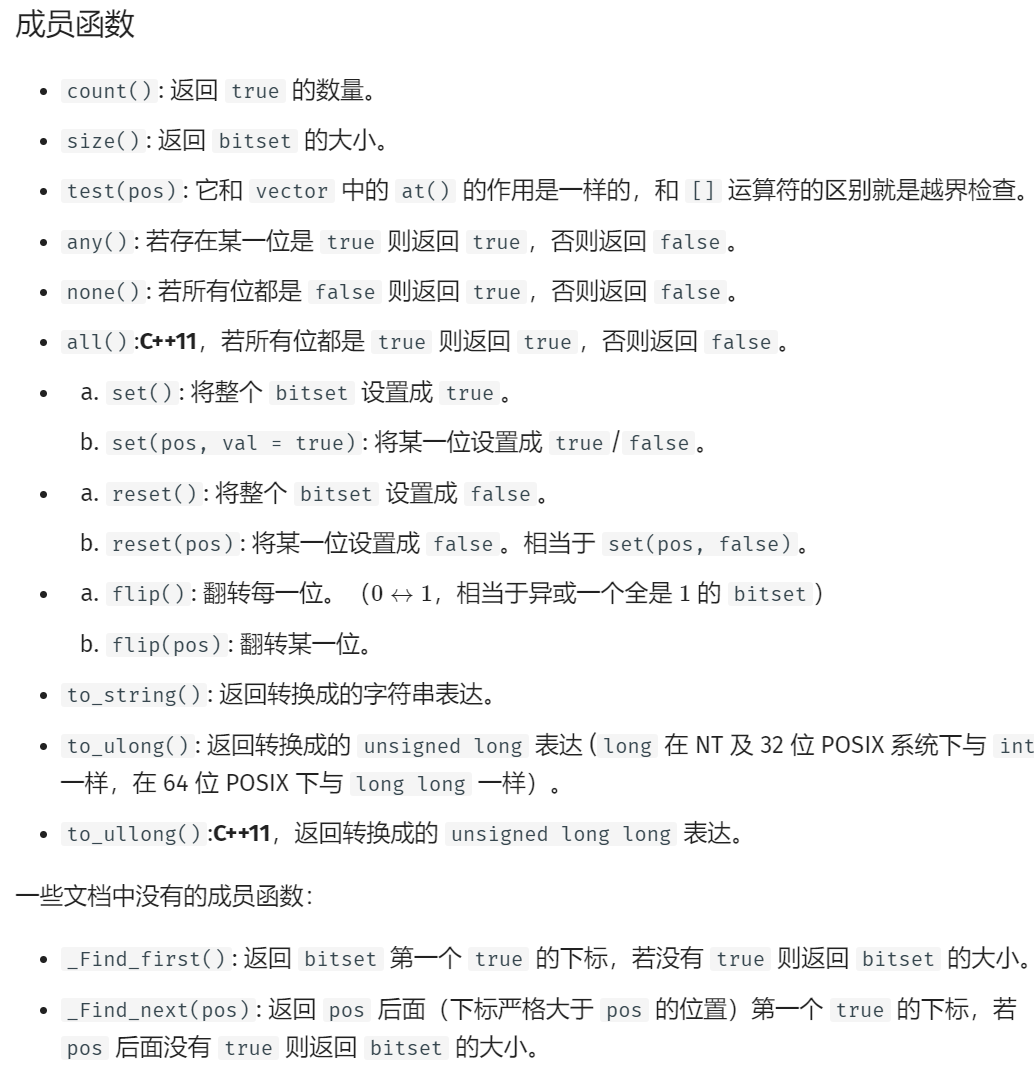
\includegraphics[width=10cm]{images/bitset.png}
\end{figure}

% manacher
\section{Manacher 算法}
\begin{itemize}
    \item $r[i]$: 以 $i$ 为回文中心的回文串半径
    \item $pre[i]$: 以 $i$ 为起点的回文串数量
    \item $suf[i]$: 以 $i$ 为终点的回文串数量
\end{itemize}
\textbf{对于一个字符串 $s$ ,它的本质不同回文子串个数最多只有$|s|$个}
\begin{minted}{c++}
namespace Manacher {
    int r[maxn << 1], pre[maxn << 1], suf[maxn << 1], l, len;
    char str[maxn << 1];
    // r[i]新串以i为中心的回文半径 r[i]-1对应一个原串回文长度
    int init(char *s) {
        str[0] = '$', str[1] = '#', len = 2, l = strlen(s);
        for (int i = 0; i < l; i++)
            str[len++] = s[i], str[len++] = '#';
        str[len] = 0;
        return len; // 返回构造的字符串长度
    }

    int solve() {
        int ans = -1, id = 0, mx = 0;
        for (int i = 1; i < len; i++) {
            r[i] = (i < mx) ? min(r[2 * id - i], mx - i) : 1;
            while (str[i - r[i]] == str[i + r[i]])
                r[i]++;
            if (mx < i + r[i])
                mx = i + r[i], id = i;
            ans = max(ans, r[i] - 1);
        }
        return ans; // 返回最长回文半径
    }

    void calc() {
        for (int i = l * 2, x; i >= 2; i--)
            x = i / 2, pre[x]++, pre[x - (r[i] / 2)]--;
        for (int i = l; i >= 1; i--)
            pre[i] += pre[i+1];
        for (int i = 2, x; i <= l * 2; i++)
            x = (i + 1) / 2, suf[x]++, suf[x + (r[i] / 2)]--;
        for (int i = 1; i <= l; i++)
            suf[i] += suf[i-1];
    }
 }
\end{minted}

% AC 自动机
\section{AC 自动机}

\par 在 Trie 树的基础上,为节点增加 fail 指针;当前节点失配的时候,将匹配指针转移到 fail 指针指向的节点。
\vspace{0.5em}

\par\textbf{建树}
\begin{itemize}
    \item 根节点指向的所有节点的 $fail$ 指针都指向根节点
    \item 不存在的节点,$fail$ 指针指向根节点
    \item 普通节点,字符为 $s$ 的 $fail$ 指针,指向它的父节点的 $fail$ 指针指向节点 $fail[p]$ 沿 $s$ 走到的节点。
\end{itemize}

\par\textbf{匹配}
\begin{itemize}
    \item 如果走到了不存在的节点,则将匹配指针移到 fail 指针指向的节点
    \item 从根节点开始匹配,原理与 Trie 树相同,匹配指针沿着 $p[i]$ 所在的字母向下走
    \item 如果失配,则沿着 fail 指针移动,若匹配上则继续匹配,否则不断沿着 fail 指针走。
\end{itemize}

\par\textbf{Fail 指针}
\begin{itemize}
    \item 每个节点 $s$ 有一个失配指针 $p$ ,所有的 $s$ 和它们的 $p$ 构成的树形结构称为 fail 树。
    \item fail 树上每个节点所代表的字符串,是其所有子树所代表的字符串的后缀 ⇒ 一个节点所有祖先,代表的字符串都是这个节点代表的字符串的后缀,如下图所示。
    \item 重要性质:每个节点的 fail 指针,都指向当前节点代表的字符串的最长后缀(如果存在)。
\end{itemize}

\par\textbf{Fail 指针的用法}
\begin{itemize}
    \item 统计每个模式串 p 在文本串 t 当中出现的次数:将 t 在 AC 自动机的上匹配同时建立 fail 树,当经过某个节点时,对答案的贡献为:这个节点所有祖先的权值之和。利用树上差分将经过的所有节点计数 + 1。
    \item 一个模式串 $p_i$ 在其它模式串中出现的次数统计:如果 $p_i$ 在其它的模式串中出现,那么其它模式串的链上一定有一个节点的 fail 指针指向该节点,直接统计该节点在 fail 树上的子节点个数即可。
\end{itemize}



\begin{minted}{c++}
namespace ACAM { 
    struct Trie {
        int ch[26],fail,cnt;
    }trans[N];
    int ins(char *s) {
        int p=0;
        for(int i=0;s[i];i++) {
            int c=s[i]-'a';
            if(!trans[p].ch[c]) trans[p].ch[c]=++cnt;
            p=trans[p].ch[c];
        }
        return p;
    }
    void getfail() {
        queue<int> q;
        for(int i=0;i<26;i++)
            if(trans[0].ch[i]) q.push(trans[0].ch[i]);
            
        while(q.size()) {
            int u=q.front();q.pop();
            for(int i=0;i<26;i++) {
                int &ch=trans[u].ch[i];
                if(ch) // add(trans[ch].fail,ch);// 构建失配树 fail指针向自己连边
                    trans[ch].fail=trans[trans[u].fail].ch[i],q.push(ch);
                else// 如果没有儿子 那么将fail的儿子作为儿子
                    ch=trans[trans[u].fail].ch[i];  
            }
        }
    }
    // t在AC自动机中跑一遍
    void find (char *t) { 
        int n = strlen(t + 1);
        for (int i = 1, p = 0; i <= n; i++) {
            int c = t[i] - 'a';
            p = trans[p].ch[c];
            // ......
        }
    }
}
\end{minted}

字符集较大的情况:可以用map来维护 tran[N][26] ,也可以用可持久化数组维护map<int,int> trans[N]

\begin{minted}{c++}
vector<pair<int,int>> trie[N]; // trie树的结构,邻接表vector
map<int,int> trans[N];
int fail[N];
void getfail()
{
    queue<int>q;
    for(auto it:trie[0]) {
        int u=0,v=it.second,to=it.first;
        // u-(to)-> v
        trans[u][to]=v;
        fail[v]=u;
        q.push(v);
    }
    while(!q.empty()) {
        int u=q.front(); q.pop();
        trans[u]=trans[fail[u]];//先把fail的trans 复制移过来
        
        for(auto it:trie[u]) {
            int v=it.second,to=it.first;
            trans[u][to]=v; // 然后修改
            fail[v]=trans[fail[u]][to]; 
            q.push(v);
        }
    }
}
// 可持久花数组维护map<int,int> trans[N]
struct Node {
    int l,r,v;
}trans[N*40];// 1~n trans[u][1~n] = v
int rt,cnt;
\end{minted}
给定 $n$ 个字符串 $s_{1 \dots n}$。, $q$ 次询问 $s_{l \dots r}$ 在 $s_k$ 中出现了多少次。$n,q,\sum_{i=1}^n |s_i| \le 10^5$。
\begin{tcolorbox}

\par \noindent 出现多串一定要考虑一下根号分治。

\begin{itemize}
\item 对于 $|s_k| < B$ 的,可以在 ac 自动机上暴力跑,差分一下用扫描线求一下,需要一个 $O(\sqrt N) - O(1)$ 的数据结构。
\item 对于 $|s_k| \geq B$ 的,这样的串不会有很多种,对于每种,把该串在ac自动机上的路径加1,然后计算子树和就可获得每个点在该串的出现次数。
\end{itemize}
\par \noindent 总复杂度 $O(n\sqrt n)$

\end{tcolorbox}

\begin{minted}{c++}
// 1. s[k]在 s[l~r]出现多少次
// 2. s[l~r]在 s[k] 中共出现多少次

// 如何理解 s[k] 在 s[r] 中出现的次数

// 1. 修改:s[r]的子串是根到 pos[r] 的链 + 1
//    查询:pos[k]子树即可               差分 + 扫描线

// 2. 修改:将 pos[k] 的子树打上标记 
//    查询:根到 pos[r] 的链上有多少标记 差分 + 扫描线 

#include <bits/stdc++.h>
using namespace std;


using LL = long long;
using PII = pair<int, int>;

const  int N = 1000005;
struct ACAM{
  int ch[N][26], cnt = 1, q[N], fa[N], head[N], ne[N];
  int ins(int p, int x) {
    if (!ch[p][x]) ch[p][x] = ++cnt;
    return ch[p][x];
  }
  void build() {
    int l, r;
    q[l = r = 1] = 1;
    while (l <= r) {
      int x = q[l++];
      if (x > 1 && !fa[x]) fa[x] = 1;
      for (int i = 0; i < 26; i++) {
        int &y = ch[x][i], z = ch[fa[x]][i];
        if (y) {
          q[++r] = y, fa[y] = z;
        } else {
          y = z;
        }
      }
    }

    for (int i = 2; i <= r; i++) {
      int x = fa[q[i]];
      assert(x);
      ne[i] = head[x], head[x] = i;
    }
    dfs(1);
  }

  int in[N], out[N], dfn;
  void dfs(int x) {
    in[x] = dfn++;
    for (int i = head[x]; i; i = ne[i]) {
      dfs(q[i]);
    }
    out[x] = dfn;
  }

  int val[N];
  void clear() {
    memset(val, 0, cnt + 1 << 2);
  }
  void cal() {
    for (int i = cnt; i; i--) {
      val[fa[q[i]]] += val[q[i]];
    }
  }
} ac;

template <class T>
struct DS {
  T s0[N], s1[(N >> 8) + 1];
  void add(int l, int r, const T &x) {
    while (l & 255 && l < r) s0[l++] += x;
    while (l + 256 <= r) s1[l >> 8] += x, l += 256;
    while (l < r) s0[l++] += x;
  }
  T ask(int p) {
    return s0[p] + s1[p >> 8];
  }
};

DS<int> ds;

int n, m, pos[N];
string s[N];
int main() {
  
  ios::sync_with_stdio(false);
  cin.tie(nullptr);
  cin >> n >> m;
  for (int i = 1; i <= n; i++) {
    cin >> s[i];
    int p = 1;
    for (char c : s[i]) {
      p = ac.ins(p, c - 'a');
    }
    pos[i] = p;
  }

  vector<LL> ans(m);
  vector<array<int, 4>> q0, q1;
  for (int i = 0, l, r, k; i < m; i++) {
    cin >> l >> r >> k;
    if (s[k].size() < 350) {
      q0.push_back({r, 1, k, i});
      q0.push_back({l - 1, -1, k, i});
    } else {
      q1.push_back({k, l, r, i});
    }
  }

  sort(q0.begin(), q0.end());
  sort(q1.begin(), q1.end());

  ac.build();
  
  for (int i = 0, j = 1; i < q0.size(); i++) {
    while (j <= q0[i][0]) {
      int x = pos[j++];
      ds.add(ac.in[x], ac.out[x], 1);
    }
    int p = 1;
    LL res = 0;
    for (char c : s[q0[i][2]]) {
      p = ac.ch[p][c - 'a'];
      res += ds.ask(ac.in[p]);
    }
    ans[q0[i][3]] += q0[i][1] * res;
  }

  vector<LL> sum(n + 1);
  for (int i = 0; i < q1.size(); i++) {
    auto &[k, l, r, id] = q1[i];
    if (!i || q1[i - 1][0] != k) {
      ac.clear();
      int p = 1;
      for (char c : s[k]) {
        p = ac.ch[p][c - 'a'];
        ac.val[p]++;
      }
      
      ac.cal();     // 子树求和
      // ac.val[pos[j]] 是 s[j] 在 s[k] 出现的次数
      for (int j = 1; j <= n; j++) {
        sum[j] = sum[j - 1] + ac.val[pos[j]];
      }
    }
    ans[id] = sum[r] - sum[l - 1];
  }

  for (auto z : ans) cout << z << "\n";
  return 0;
}
\end{minted}

% 后缀数组
\section{后缀数组}

\subsection{模板}
\begin{itemize}
    \item $sa[i]$:排名为 $i$ 的后缀的起始下标(排第 $i$ 的是哪个后缀)
    \item $rank[i]$:起始下标为 $i$ 的后缀 $suffix(i ... len-1)$ 的排名(第 $i$ 个后缀排第几),满足 $sa[rank[i]] = i, rank[sa[i]] = i$.
    \item $height[i]$: $sa[i]$ 与 $sa[i-1]$(排名相邻的两个后缀) 的最长公共前缀。
    \item $h[i] = height[rank[i]]$: $suffix(i)$ 和在他前一名的后缀的最长公共前缀。满足 $h[i] \ge h[i-1] - 1$.
\end{itemize}

\begin{minted}{c++}
namespace Suffix_Array {
    // sa[i]: 排名是i位的是第几个后缀
    // rk[i]: 第i个后缀的排名是多少
    // height[i]: sa[i]与sa[i-1]
    const int N=1000010;
    char s[N];
    int rk[N],sa[N],c[N],height[N];
    int x[N],y[N];
    int n,m;
    void rsort()// x[i] 第一关键字 y[i] 第二关键字 基数排序
    {
        for(int i=1;i<=m;i++) c[i]=0;
        for(int i=1;i<=n;i++) c[x[i]]++;
        for(int i=1;i<=m;i++) c[i]+=c[i-1];
        for(int i=n;i;i--) sa[c[x[y[i]]]--]=y[i];
    }
    void build_sa()
    {
        n=strlen(s+1);
        m=256;
        for(int i=1;i<=n;i++) x[i]=s[i],y[i]=i;
        rsort();
        for(int k=1;k<=n;k<<=1)
        {
            int p=0;
            for(int i=n-k+1;i<=n;i++) y[++p]=i;// 第二关键字为空字符排在最前面
            for(int i=1;i<=n;i++) if(sa[i]>k) y[++p]=sa[i]-k;
            rsort();swap(x,y);
    
            x[sa[1]]=1,p=1;
            for(int i=2;i<=n;i++)
                x[sa[i]]=(y[sa[i]]==y[sa[i-1]]&&y[sa[i]+k]==y[sa[i-1]+k]?p:++p);
            if(p==n) break;
            m=p;
        }
    }
    void get_height()
    {
        for(int i=1;i<=n;i++) rk[sa[i]]=i;
        // 求height
        for(int i=1,j=0;i<=n;i++)
        {
            if(j) --j;
            while(s[i+j]==s[sa[rk[i]-1]+j]) j++;
            height[rk[i]]=j;
        }
    }
    // 求lcp 有时需要找到本质不同第k大最早出现的位置
    // 首先二分能找到第k大,然后再次二分找到[sa[l]....sa[r]] 取最小值就是最早出现的位置
    int mnht[N][22];
    int mnsa[N][22];
    int lg[N];
    void init() {
        lg[0]=-1;
        for(int i=1;i<=n;i++) lg[i]=lg[i>>1]+1;
        for(int i=1;i<=n;i++) mnht[i][0]=height[i],mnsa[i][0]=sa[i];
        for(int j=1;j<=lg[n];j++)
            for(int i=1;i+(1<<j)-1<=n;i++)
                mnht[i][j]=min(mnht[i][j-1],mnht[i+(1<<j-1)][j-1]),\
                mnsa[i][j]=min(mnsa[i][j-1],mnsa[i+(1<<j-1)][j-1]);
    }
    int MIN(int a[][22],int l,int r)
    {
        int k=lg[r-l+1];
        return min(a[l][k],a[r-(1<<k)+1][k]);
    }
    // 询问 suffix(a) 和 suffix(b) 的最长公共前缀
    int lcp(int a,int b) 
    {
        a=rk[a],b=rk[b];
        if(a>b) swap(a,b);
        a++;
        int k=lg[b-a+1];
        return min(mnht[a][k],mnht[b-(1<<k)+1][k]);
    }
    
}using namespace Suffix_Array;
\end{minted}
\subsection{SA 应用}
\subsubsection{寻找最小的循环移动位置}
\par \noindent 
\begin{tcolorbox}
\par \noindent P4051 [JSOI2007]字符加密:给出一个字符串S,将该字符串循环移位后的$n$个字符串按照字典序排列,输出排序后的每个尾字符。

\end{tcolorbox}
\par \noindent  将字符串 S 复制一份变成 SS 就转化成了后缀排序问题。
 
\subsubsection{在字符串中找子串}
\begin{tcolorbox}
\par \noindent 任务是在线地在主串 S 中寻找模式串 P。在线的意思是,我们已经预先知道主串 S,但是当且仅当询问时才知道模式串 P。
\end{tcolorbox}
\par \noindent 构造出 S 的后缀数组,若 P 在 S 的子串出现,必定是 S 的后缀的前缀,因为已经将 S 的后缀按照字典序排序了,既可以二分 sa[mid] 数组,比较 S 排名是`mid`的后缀和 P 的字典序大小,比较复杂度为 $O(|P|)$,每次查找的复杂度为 $O(|P|\log |S|)$。
~\\
\par \noindent 注意,如果该子串在 S 中出现了多次,每次出现都是在 sa 数组中相邻的。因此出现次数可以通过再次二分找到,输出每次出现的位置也很轻松。

\subsubsection{两子串最长公共前缀}
\begin{tcolorbox}
\par \noindent 求后缀$S_{i\to n}$ 和 $S_{j\to n}$的最长公共前缀 $\text{lcp}(i,j)$
\end{tcolorbox}

$$\text{lcp}(i,j)=\min\{\text{height}[rk[i]+1,\dots,rk[j]\}$$


\par \noindent 如果 height 一直大于某个数,前这么多位就一直没变过;反之,由于后缀已经排好序了,不可能变了之后变回来(height一旦减小,就会有别的字符替代,而且由于字典序的问题是不可逆的)。有了这个定理,求两子串最长公共前缀就转化为了 RMQ 问题。

\subsubsection{比较一个字符串的两个子串的大小关系}

\begin{tcolorbox}
\par \noindent 假设需要比较的是 $A=S[a...b]$ 和  $B=S[c...d]$ 的大小关系。
\end{tcolorbox}
\par \noindent 若$\text{lcp}(S[a...n],S[c...n])>\min(|A|,|B|)$,则$A<B \Leftrightarrow |A| <|B|$ ,否则$A<B \Leftrightarrow \text{rk}[a] <\text{rk}[c]$ 

\subsubsection{不同子串的数目}
\par \noindent 
\par \noindent \textbf{子串就是后缀的前缀},所以可以枚举每个后缀,计算前缀总数,再减掉重复。
~\\
\par \noindent “前缀总数”其实就是子串个数,为$n(n+1)/2$。
~\\
\par \noindent 如果按后缀排序的顺序枚举后缀,每次新增的子串就是除了与上一个后缀的 LCP 剩下的前缀。只有这些前缀是新增的,因为 LCP 部分在枚举上一个前缀时计算过了。

\subsubsection{出现至少 K 次的子串的最大长度}
\par \noindent 
\par 出现至少 k 次意味着后缀排序后有至少连续 $k$ 个后缀的 LCP 是这个子串。所以,求出每相邻 $k-1$ 个 height 的最小值,再求这些最小值的最大值就是答案。\par 
\subsubsection{至少出现两次且不重叠的最长子串}
\par \noindent 若可重叠,答案就是$\max\{height[i]\}$
~\\
\par \noindent \textbf{二分目标串的长度} $|S|$,将 $\text{height}$ 数组划分成若干个连续 LCP 大于等于$|S|$ 的段,利用 RMQ 对每个段求其中出现的数中最大和最小的下标,若这两个下标的距离满足条件(不重叠),则一定有长度为 $|S|$ 的字符串不重叠地出现了两次。

\subsubsection{结合并查集}
\par \noindent 
\par \noindent 某些题目求解时要求你将后缀数组划分成若干个连续 LCP 长度大于等于某一值的段,亦即将 $\text{height}$ 数组划分成若干个连续最小值大于等于某一值的段并统计每一段的答案。
~\\
\par \noindent 如果有多次询问,我们可以将询问离线。观察到当给定值单调递减的时候,满足条件的区间个数总是越来越少,而新区间都是两个或多个原区间相连所得,且新区间中不包含在原区间内的部分的 $\text{height}$ 值都为减少到的这个值。我们只需要维护一个并查集,每次合并相邻的两个区间,并维护统计信息即可。
\subsubsection{结合单调栈}
\par \noindent 
\begin{tcolorbox}
\par [AHOI2013]差异:给定一个长度为 $n$ 的字符串 $S$,令 $T_i$ 表示它从第 $i$ 个字符开始的后缀。求
$$ \sum_{1\leq i<j\leq n}\text{len}(T_i)+\text{len}(T_j)-2\times\text{lcp}(T_i,T_j)$$
\par 其中,$\text{len}(a)$ 表示字符串 $a$ 的长度,$\text{lcp}(a,b)$ 表示字符串 $a$ 和字符串 $b$ 的最长公共前缀。
\end{tcolorbox}

\par \noindent 被加数的前两项很好处理,为 $(n-1)n(n+1)/2$ (每个后缀都出现了 $n-1$ 次,后缀总长是 $n(n+1)/2$),关键是最后一项,即后缀的两两 LCP。
~\\
\par 我们知道  $\text{lcp}(i,j)=k$ 等价于 $\text{lcp}(i,j)=\min\{\text{height}[i+1,...,j]\}=k$。
~\\
\par 考虑 Height 数组的贡献:Height 数组中 $[2, n]$ 内的每一个区间都给答案贡献区间最小值。
~\\
\par \noindent 我们换一个角度来思考:如果设$\min\{\text{height}[i+1,...,j]\}=\text{height}[k]$,那么我们认为$\text{height}[k]$ 产生了一个贡献,所以我们可以从每一个 $\text{height}[k]$ 产生了多少贡献的角度来思考。
~\\
\par \noindent  \textbf{套路:每个区间的区间最小值之和,使用单调栈解决。},注意单调栈,寻找时左闭右开 $[ \dots)$

\begin{minted}{c++}
 // L[i]表示左侧第一个<=height[i]的位置
    q[tt=0]=1;
    for(int i=2;i<=n;i++)
    {
        while(tt&&height[q[tt]]>height[i]) tt--;
        L[i]=q[tt];
        q[++tt]=i;
    }
    // R[i] 表示右侧第一个<height[i]的位置
    q[tt=0]=n+1;
    for(int i=n;i>=2;i--) 
    {   
        while(tt&&height[q[tt]]>=height[i]) tt--;
        R[i]=q[tt];
        q[++tt]=i;
    }   
    for(int i=2;i<=n;i++) (R[i]-i)*(i-L[i])*height[i];
\end{minted}
\subsubsection{求本质不同第 K 大子串}
\par \noindent 首先第 $k$ 大可以二分,对后缀排序后,先二分定位第 $k$ 大属于哪一个后缀(后缀的前缀是子串)
~\\
\par \noindent 按照经典的,把重复的子串算在排名靠前的后缀中,排名为 $i$ 的后缀对总子串(不同)的贡献是 $n-sa[i]+1-\text{height}[i]$,然后预处理一个前缀和就可以二分第 $k$ 大 “大致” 属于哪一个后缀,甚至可以直接确定子串。
~\\
\par \noindent 不过本题要求输出子串最早出现的位置(左右端点确定一个子串)。
~\\
\par \noindent 上述求的该串的\textbf{开始位置}不一定是\textbf{下标最小}的,所以顺着sa数组要往后找是否还有更小的答案。(因为排名 $i,i+1$ 的子串有lcp)
\begin{minted}{c++}
int l=j,r=n;
while(l<r)
{
    int mid=l+r+1>>1;
    if(MIN(mnht,j+1,mid)>=q[i].l) l=mid;
    else r=mid-1;
}
j=MIN(mnsa,j,r);
\end{minted}
\subsubsection{重复次数最多的连续子串}
\begin{tcolorbox}
\par \noindent 给一个串,一段(连续)子串称为 $(k,l)$ 重复的,如果它满足由一个长度为 $l$ 的重复了 $k$ 次组成。求最大的 $k$
\end{tcolorbox}
\par \noindent 枚举答案子串长度 $L$,在 $\frac{N} {L}$ 个关键点中,答案子串必须覆盖相邻的2个点。枚举相邻的关键点 $j$ 和 $j+L$,看它们往前往后各能匹配到多长。将反串接在原串后一起求SA,用lcp信息更新 ans:
\begin{figure}[H]
        \centering
        \par 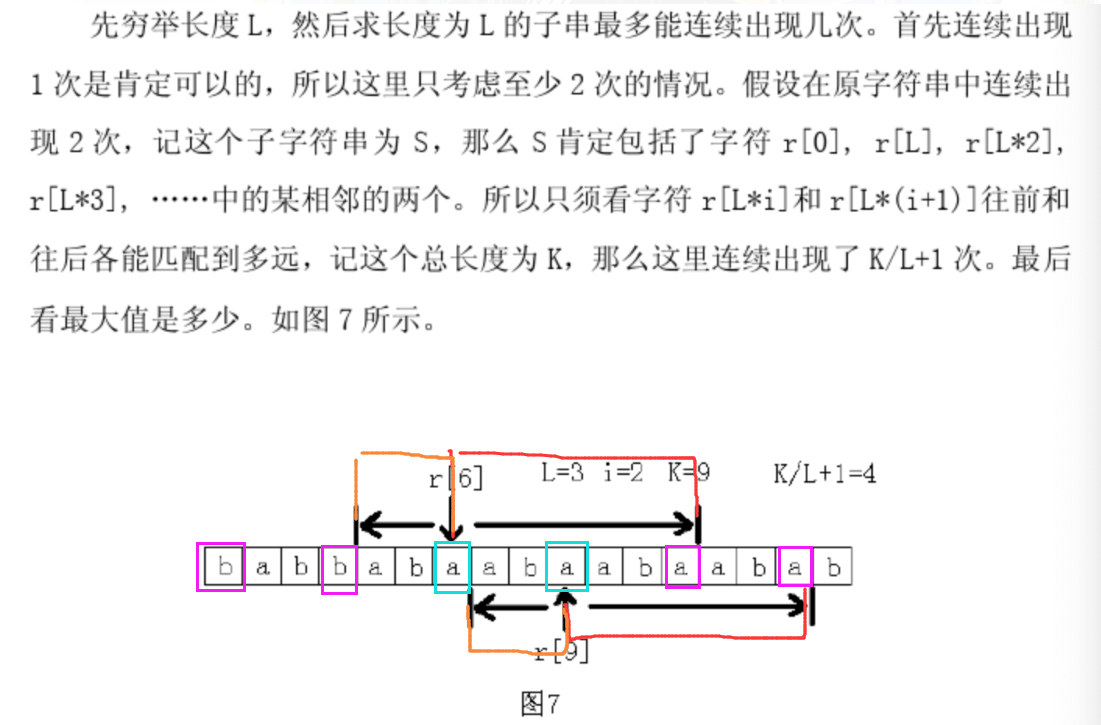
\includegraphics[width=10cm]{images/repeats.png}
\end{figure}
\par \noindent 具体的枚举长度 $L=2$ 时,上图紫色和青色是关键的的位置,考虑两个青色的(相邻)关键点,红色部分是往后扩展的长度,橘色部分是往前扩展的长度(正反串的 $\text{lcp}(j, j+L)$ )然后加起来就是循环长度。

\begin{minted}{c++}
ans = max(ans, (lcp(j, j+i)+lcp(N-j+1,N-(j+i)+1)+i-1)/i);
\end{minted}
\subsubsection{其他}
\begin{itemize}
    \item 求某两个后缀的最长公共前缀:$suffix(j)$ 和 $suffix(k)$ 的最长公共前缀为:$min\{height[rank[j] + 1], height[rank[j] + 2], ... height[rank[k]]\}$;这是一个 RMQ 问题,可以用 ST 表$O(nlogn)$ 预处理,$O(1)$ 查询。
    \item 可重叠最长重复子串:子串一定是某个后缀的前缀;可重叠的子串则等价于求两个后缀的最长公共前缀,所以求 $height[]$ 数组的最大值即可。
    \item 不可重叠最长重复子串:首先在 $[1...max(height)]$ 区间二分答案 $k$,判断是否存在两个长度为 $k$ 的子串是相同且不重叠的。利用 $height$ 值对后缀分组,使得每组的 $height$ 值都不小于 $k$(如果不存在就单独分组)。有希望成为最长公共前缀不小于 k 的两个后缀一定在同一组。然
    后对于每组后缀,只须判断每个后缀的 $sa$ 值的最大值和最小值之差是否不小于 $k$。
    \item 可重叠并出现 $k$ 次的最长重复子串:同样先二分长度答案 $x$ 分成若干组,判断的是有没有一个组的后缀个数不小于 $k$. 如果存在则满足条件。
    \item 不相同的子串个数:因为子串一定是某个后缀的前缀,问题等价于求所有后缀之间不相同的前缀的个数,如果所有的后缀按照 $suffix(sa[i])$ (排名)的顺序计算,对于新加入的后缀 $suffix(sa[k])$,将贡献 $n - sa[k] + 1 - height[k]$ 个不同的子串,累加即可。
    \item 最长回文子串:将整个字符串反过来接在原字符的后面,中间用一个特殊的字符隔开,求新字符串某两个后缀的最长公共前缀即可。
    \item 连续重复子串:(定义:字符串 $L$ 由某个字符串 $S$ 重复 $r$ 次得到,则 $L$ 称为连续重复子串)
    \item 求 $r$ 的最大值:枚举字符串 $S$ 的长度 $k$,然后判断是否满足。判断时先看 $L$ 的长度能否被 $k$ 整除,再看 $suffix(1)$ 和 $suffix(k+1)$ 的最长公共前缀是否等于 $n-k$,如果是则合法。
    \item 重复次数最多的连续重复子串:首先预处理 LCP;枚举重复部分的长度 $l$,然后枚举每一个起始位置$i$。如果重复部分出现大于等于 2 次,那么一定会有 $s[0], s[l], s[2*l]...s[k*l]$ 其中两个连续出现在重复组成的串中。所以对于确定的长度,$O(1)$ 查询 $s[i]$ 和 $s[i+l]$ 的公共前缀,然后向前向后匹配,重复串长度即为 $lcp(i, i + l) + (l - k \% l)$,然后再检查一下起点 $t=i-l+k\%l$ 是否溢出,以及 $lcp(t, t+l)$ 的长度是否大于 $k$ 即可更新答案。时间复杂度为 $O(nlogn)$.
    \item $A,B$ 的最长公共子串:首先把 $B$ 连接到 $A$ 的末尾,两者中间用一个没出现过的字符(如\$隔开),然后求新串的后缀数组、height 数组等。然后遍历 height 数组,当 $suffix(sa[i])$ 和 $suffix(sa[i-1])$ 不是同一个字符串中的两个后缀时,最大的$height[i]$就满足条件。判断 $suffix(sa[i])$ 和 $suffix(sa[i-1])$ 是否为同一个字符串中的两个后缀,只需判断下标的位置即可。
    \item $A,B$ 的长度不小于 $k$ 的公共子串个数(可以相同):思路是计算 A, B 的所有后缀之间的 lcp 的长度,统计 $lcp \ge k$ 的答案。首先把 $B$ 连接到 $A$ 的末尾,两者中间用一个没出现过的字符(如\$隔开),计算 height 后按 height 值大于等于 $k$ 分组。然后将后缀扫描一遍,遇到一个 B 的后缀就统计与前面的 A 的后缀能产生多少个长度不小于 $k$ 的公共子串。A 的后缀可以用单调栈维护;然后将 A 用相同的办法统计一次。
    \item 给定 $n$ 个字符串,求出现在不小于 $k$ 个字符串中的最长子串:将 $n$ 个字符串连接,中间用没出现过的字符隔开,求后缀数组。然后二分长度 $l$ 并利用 $height$ 数组分组,判断每组的后缀是否出现在不小于 $k$ 个原串中。
    \item 给定 $n$ 个字符串,求在每个字符串中至少出现两次且不重叠的最长子串:和上面一样,判断的时候,要看是否有一组后缀在每个原来的字符串中至少出现两次,并且在每个原来的字符串中,后缀的起始位置的最大值与最小值之差是否不小于当前答案(判断能否做到不重叠,如果题目中没有不重叠的要求,那么不用做此判断).
    \item 给定 $n$ 个字符串,求出现或反转后出现在每个字符串中的最长子串:将每个字符串反转后的结果也拼到总串中,求后缀数组。判断的时候,要看是否有一组后缀在每个原来的字符串或反转后的字符串中出现.
\end{itemize}

\clearpage

% 后缀自动机
\section{后缀自动机}
处理与子串相关问题的在线线性算法。
\paragraph{名词解释}
\begin{itemize}
\item  $len$ 表示从当前 $endpos$ 可向前延伸的长度最大值。设当前构造的 $SAM$ 已得到的子串为 $s$, 从当前字符向前数 $[0, len]$ 个字符得到的新子串 $t$,$t$ 一定只作为 $s$ 的后缀出现。
\item 如:对于母串 $abcdabcdbbcd$, 有三个子串 $d, cd, bcd$ 的 $endpos$ 集合相同,而从 $endpos$ 向前最多可以延伸 $3$ 个字符满足条件,所以 $len = 3$.
\item  $link$ 表示后缀连接。定义一个子串 $v \in endpos(v)$ ($endpos(v)$ 称为 $v$ 的 endpos 等价类),该等价类中长度最长的子串为 $w$, 则 $w$ 的“最长的且不在该 endpos 等价类中的后缀”记为 $t$,令 $link(v) = t$.
\item 如:对于母串 $abcdabcdcd$, $abcd, bcd$ 在同一个 endpos 等价类中。设 $v = bcd$, 则显然 $w = abcd$, $w$ 的最长的且不再该等价类中的后缀显然为 $cd$,则令 $link(bcd) = cd$. Tips: 后缀也有长度为 0 的情况,即空后缀。
\item  $nxt[i]$ 就是沿着字符 $'a' + i$ 走可以到达的下一个状态。
\end{itemize}

\paragraph{性质}

\begin{itemize}
\item 字符串 $s$ 的一个后缀自动机包含关于字符串 $s$ 的所有子串的信息。任意从初始状态 $t_0$ 开始的路径,如果我们将转移路径上的标号写下来,都会形成 $s$ 的一个 子串 。反之每个 $s$ 的子串对应从初始状态 $t_0$  开始的某条路径。
\item 每个状态 $s$ 代表的子串是区间 $[len_{link(s)}+1, len_s]$.
\item 一个长度为 $n$ 的字符串,它的 SAM 节点个数最多有 $2n-1$ 个,连边最多有 $3n-4$ 条。
\item 树形结构的性质:设字符串长度为 $n$,考虑 extend 操作中 $cur$ 变量的值(代表当前状态在节点池中的下标),该节点对应的状态是:执行 extend 操作时的当前字符串,得到的 $n$ 个节点对应了$n$ 个不同的终点,第 $i$ 个状态对应 $S_{1...i}$。如果我们将 SAM 看作一棵树,树根为 $0$ 号节点(初始状态),其余节点 $v$ 满足其父亲为该节点的后缀连接 $link(v)$。这棵树叫 $parent$ 树。
\item $parent$ 树中的每个节点的终点集合,等于其子树内所有终点节点对应的终点集合的并集。
\item $parent$ 树中,如果节点 $a$ 是 $b$ 的祖先,则节点 $a$ 对应的字符串是节点 $b$ 对应的字符串的后缀。
\item 构成的 $parent$ 树存在一些与树相关的性质,如 $S_{1...p}$ 和 $S_{1...q}$ 的最长公共后缀对应的是 $p, q$ 对应节点间的 LCA 的字符串。
\item 除了初始状态(节点 $0$)以外,每个状态 $i$ 对应的字串数量是 $len(i) - len(link(i))$,因此计算时可以自上而下计算。
\end{itemize}

\begin{minted}{c++}
namespace SuffixAutomaton {
    const int maxn = 200050;
    const int MAXLOG = 25;
    // 需要维护 right 集合时,加上以下动态开点线段树的代码
    struct Node {
        int val, l, r;
    } t[maxn * 40];
    int cnt;        // 权值线段树节点个数

    void pushup(int u) {
        t[u].val = t[t[u].l].val + t[t[u].r].val;
    }
    void update(int &u, int l, int r, int pos) {
        if (!u)
            u = ++cnt, t[u].l = t[u].r = t[u].val = 0;
        if (l == r) {
            t[u].val++;
            return;
        }
        int mid = (l + r) >> 1;
        if (pos <= mid)
            update(t[u].l, l, mid, pos);
        else
            update(t[u].r, mid + 1, r, pos);
        pushup(u);
    }
    int merge(int x, int y) {
        if (!x || !y)
            return x + y;
        int o = ++cnt;
        t[o].l = merge(t[x].l, t[y].l);
        t[o].r = merge(t[x].r, t[y].r);
        pushup(o);
        return o;
    }

    int query(int u, int l, int r, int L, int R) {
        if (!u) return 0;
        if (L <= l && r <= R) return t[u].val;
        int mid = l+r>>1;
        int v = 0;
        if (L < =mid) v += query(t[u].l, l, mid, L, R);
        if (R > mid) v += query(t[u].r, mid+1, r, L, R);
        return v;
    }
    /* 后缀自动机 */
    struct State {
        int len, link, ch[26];
        State(int _len = 0, int _link = 0): len(_len), link(_link) {
            memset(ch, 0, sizeof ch);
        }
    } st[maxn << 1];    // 最多有 2n-1 个节点,开两倍空间

    // tot: 状态个数,last: 上一次插入的字符对应状态,sum:当前产生子串个数,n 字符串长度
    // sa c 基数排序数组, endpos[i] 表示 i 状态所代表的 endpos 集合线段树的树根
    int last, tot;
    int n, sum;
    int endpos[maxn << 1], sa[maxn << 1], c[maxn << 1], pos[maxn << 1];
    int f[maxn << 1][MAXLOG];
    int ans[maxn << 1];
    int extend(int c, int idx) {
        int p = last;
        int np = last = ++ tot;
        
        st[np] = State(st[p].len + 1);
        ans[np] = 1;

        endpos[np] = 0;
        update(endpos[np], 1, n, idx);  // 更新当前点的 endpos,注意权值线段树值域范围

        for (; p && !st[p].ch[c]; p=st[p].link) st[p].ch[c] = np;
        
        if (!p) st[np].link = 1;
        else {
            int q = st[p].ch[c];
            if (st[q].len == st[p].len + 1)
                st[np].link = q;
            else {
                int clone = ++tot;
                st[clone] = State(st[p].len + 1, st[q].link);
                memcpy(st[clone].ch, st[q].ch, sizeof st[q].ch);
                
                endpos[clone] = 0;              // 为克隆节点新建 endpos,但不建树
                for (;p && st[p].ch[c] == q; p = st[p].link) st[p].ch[c] = clone;
                st[q].link = st[np].link = clone;
            }
        }
        sum += st[np].link ? st[np].len : st[np].len - st[st[np].link].len;   // 字串个数
        return sum;          
    }
    
    // 基于基数排序的拓扑排序,保证状态间的拓扑关系,即子状态在后,父状态在前
    // 后缀自动机更新信息时,需要先更新子状态 s,再更新父状态 link[s]
    void toposort() {
        memset(sa, 0, sizeof sa);
        memset(c, 0, sizeof c);
        for (int i = 1; i <= tot; i++)
            c[st[i].len]++;            // 排序的关键字是 len
        for (int i = 1; i <= tot; i++)
            c[i] += c[i-1];
        for (int i = 1; i <= tot; i++)
            sa[c[st[i].len]--] = i;
    }
    // 建立后缀自动机
    void build(char s[]) {
        n = strlen(s + 1);
        for (int i = 1; i <= n; i++) {
            extend(s[i] - 'a', i);
            pos[i] = last;
        }
        // 预处理倍增表
        for (int i = 1; i <= tot; i++) f[i][0] = st[i].link;
        for (int j = 1; j < MAXLOG; j++)
            for (int i = 1; i <= tot; i++)
                f[i][j] = f[f[i][j-1]][j-1];

        toposort();
        // 如果需要维护 right 集合:从子节点开始,合并 endpos 集合
        for (int i = tot; i > 1; i--) {
            int u = sa[i];
            if (st[u].link)
                endpos[st[u].link] = merge(endpos[st[u].link], endpos[u]);
        }
      // 按照 len 拓扑排序,能够递推求出记录每个节点的最左边出现的位置endpos和最右边出现的位置endpos。
    }
    // 询问子串 s[l,r] 在子串 s[L,R] 中出现的次数。
    int solve(int l, int r, int L, int R) {
        // 首先从 endpos 为 r 的节点开始,倍增找到与目标串一样长的点
        int u = pos[r], nplen = r - l + 1;
        for (int i = MAXLOG - 1; i >= 0; i--)
            if (st[f[u][i]].len >= nplen)
                u = f[u][i];
        return query(endpos[u], 1, n, L + r - l, R);
    }
    void init() {
        sum = 0, tot = 0,
        st[last = ++tot] = State(0, 0);
        memset(t, 0, sizeof t);     // 清空权值线段树
    }
} using namespace SuffixAutomaton;
\end{minted}

\subsection{应用}

\subsubsection{不同子串的数目}
\par \noindent SAM,其实就是统计所有状态包含的子串总数,也就是 $\sum_i \text{maxlen}[i]-\text{minlen}[i]+1$,而实际上知道$\text{minlen}[i]=\text{maxlen}[fa[i]]+1$。
~\\
\par \noindent 每个 S 的子串都相当于自动机中的以S0为起点的一些路径。因此不同子串的个数等于自动机中\textbf{以 S0 为起点的不同路径的条数}。考虑到 SAM 为有向无环图,不同路径的条数可以通过动态规划计算。具体的:即令 $d_u$ 为从状态 u 开始的路径数量(或称之不同子串数目),对于节点u,u如果通过字母c转移到了后继v,有方程:
$$
d_u=1+\sum_{(u,v,c)\in\text{DAWG}} d_v
$$
\par \noindent 可以通过dfs一下根节点向下记忆化搜索实现,也可以\textbf{逆拓扑序}往回更新实现。
~\\
\par \noindent 其实通过此我们有两种角度理解SAM上的点也就是状态
\begin{enumerate}
\item endpos:每个状态维护一些endpos相同的子串,维护的子串数量$\text{maxlen}[i]-\text{minlen}[i]+1$
\item 路径:从起点S0到该状态的一条路径唯一对映一个子串,并且路径数量等于维护的子串数量。
\end{enumerate}
\subsubsection{所有不同子串的总长度}

\par \noindent 类似的令$f_u$ 为从状态 u 开始的不同子串的总长度,对于 v 状态的所有子串都可以在前缀加上字符c,一共多出$d_v$,+1是只考虑字母c的这一条路径。(Oiwiki上没+1是因为 $d_u$ 包括空字串)
$$
f_u=1+\sum_{(u,v,c)\in\text{DAWG}} (d_v+f_v)
$$
\subsubsection{任意子串的数目}
\par \noindent 首先考虑一个子串出现的次数,不难发现就是它 endpos 集合的大小。所以我们当前需要计算的就是 $\forall st|endpos(st)|$ 的大小。如果我们每次构建时候维护这个的话,每次需要按着fa边跳到 s 更新所有状态的 endpos,然后\textbf{判断子串属于哪个状态}就能得出次数(回忆:每个状态 endpos 集合相同,endpos集合维护的是相同子串尾出现的位置)

\par \noindent 由于fa边构成一颗树,前面讲过了我们每次是暴力把路径上的所有点权值 +1 。
\par \noindent 我们就能转化成 DAG 每一个点对于它能走的路径上的所有点 +1 ,这个直接考虑在 DAG 图上进行拓扑 dp 就行了。
~\\
\par \noindent 但注意 $\text{clone}$ 的节点是不能对它到 S 的路径上有单独贡献的,因为它的贡献会在它的本体上计算一遍。
\subsubsection{字典序第 K 大子串}

\par \noindent 字典序第 K 大的子串对应于 SAM 中字典序第 K 大的路径,因此在计算每个状态的路径数后。我们可以很容易地从 SAM 的根开始找到第 K 大的路径。
~\\
\par \noindent 如果不同位置的相同子串算作多个,那么还需要提前求出任意子串的数目(建立后缀树,令前缀的cnt=1,dfs更新一遍),否则只需要让记每个状态的 cnt=1
\subsubsection{第一次出现的位置}

\begin{tcolorbox}
给定一个文本串 S,多组查询。每次查询字符串 P 在字符串 S 中第一次出现的位置( 的开头)。
\end{tcolorbox}
\par \noindent 我们构造一个后缀自动机。我们对 SAM 中的所有状态预处理位置 $\text{firstpos}$ 。即,对每个状态 u 我们想要找到第一次出现这个状态的末端的位置 $\text{firstpos}[u]$。换句话说,我们希望先找到每个集合 $\text{endpos}$ 中的最小的元素。
~\\
\par \noindent 当我们创建新状态 np 时,我们令:

$$
\text{firstpos}(np)=\text{len}(np)
$$
$$
\text{firstpos}(nq=\text{clone})=\text{len}(q)
$$
\subsubsection{最短的没有出现的字符串}

\begin{tcolorbox}
给定一个字符串 S 和一个特定的字符集,我们要找一个长度最短的没有在 S 中出现过的字符串。
\end{tcolorbox}

\par \noindent 在SAM上做dp,设 $\text{dp}[i]$表示到点 $i$ 时需要添加的最短长度的字符满足题意。如果这个点有不是S中字符的出边,则 $\text{dp}[i]=1$(添加一个未出现的字符)否则,不光要添加一个字符还需要向后继续寻找
$$
\text{dp}[i]=1+\min\{\text{dp}_{(i,j,c)\in\text{SAM}}[j]\}
$$

\par \noindent 答案就是$\text{dp}[s0]$(起点)

\subsubsection{两个串的最长公共子串}
\par \noindent 第一个串建SAM,然后一个一个串处理。在处理每一个串的时候记录当前节点的最大匹配长度,并且记录最大长度的最小值,就是所有串的匹配长度。处理串时能在自动机上走就走,否则跳fa,类似KMP和AC自动机。

\begin{minted}{c++}
int p=1,l=0;
for(int j=0;t[j];j++)
{
    int c=t[j]-'a';
    while ( p>1 && !sam[p].ch[c]) p = sam[p].fa,l = sam[p].len;
    if (sam[p].ch[c]) p = sam[p].ch[c], l++;
    len[p] = max(len[p], l);
}
\end{minted}
\subsubsection{求子串 $[l, r]$ 在子串 $[L, R]$ 的出现次数}
\par \noindent 实际上是求子串 $s[l,r]$ 的 endpos 集合中在 $[L+r-l,R]$ 出现的次数,也就是需要维护 endpos 集合,对于一个SAM状态 endpos 集合 应该是所有子树 endpos 集合的并集 + “本身的”(如果改该状态对于是一个前缀)。
\subsubsection{区间 $[l, r]$ 本质不同子串个数}

\par \noindent 考虑把本质相同的子串看作同一种颜色。「静态区间不同颜色种类数」的经典问题的加强版!
~\\
\par \noindent 插入位置 $i$ 时应该在加入所有以 $i$ 结尾的子串的贡献。子串是有长度的,但我们只需维护左端点即可。那么「在线段树中把当前位置 +1」可以直接一次区间修改来完成,而把「上一个相同元素的位置 −1」目前来看不太好做,因为我们还不知道每个子串上一次出现的位置。
~\\
\par \noindent 为了解决这个问题,我们对原串建立后缀自动机。
~\\
\par \noindent 以 $i$ 结尾的子串就是前缀 $i$ 对应的节点在 $\text{parent}$ 树上的所有祖先节点。由同一个状态表示的子串,它们「上一次出现的位置」的右端点是相同的,而左端点是连续的一段。
~\\
\par \noindent 可以通过暴力跳 $\text{parent}$ 树上祖先并同时区间修改(增删贡献)来达到目的。同时还需要把这条链上的节点都染成 $i$ 颜色,表示把这些子串最后一次出现的位置修改为 $i$。更具体的:
~\\
\par \noindent $\text{parent}$ 树上如果该节点之前被染成 $r$ 颜色,说明子串$[r-maxlen+1\to r,   r]$ 都计算过贡献,如果本次需要将其染成 $i$ 颜色 $i > r$,那么说明 $r, i$ 都是该状态的 $\text{endpos}$ 集合,并且子串 $[r-maxlen+1\to r,   r]$ 和 $[i-maxlen+1\to i,   i]$ 是本质相同的子串!
~\\
\par \noindent 离线下来扫描区间右端点然后询问左端点即可。
~\\
\par \noindent 注意:后缀自动机的状态维护:①相同结尾的连续子串 ② endpos 集合相同的子串
~\\
\par \noindent 发现颜色相同的节点的节点会连成一段,我们可以将它们一起处理。由于只有「将某一点到根节点的颜色染成一种没有出现过的颜色」这一种操作,所有需要处理的链上的总颜色数实际上是 $O(n\log n)$ 的。原因是染色操作其实对应着 LCT 的 $\text{Access}$ 操作,可以套用其复杂度证明方法。所以在实现时我们也可以直接使用 LCT 来维护,因为一条实链上的颜色一定都是相同的,直接模拟 $\text{Access}$ 的过程即可。

\subsection{LCT维护Parent树}
\begin{minted}{c++}
// P6292-区间本质不同子串个数 https://www.luogu.com.cn/problem/P6292

#include<bits/stdc++.h>

using namespace std;
using ll=long long;

const int N=200005;
struct SAM
{
    int ch[26],fa,len;
}sam[N];
int tot=1,last=1;
int extend(int c)
{   
    int p=last;
    int np=last=++tot;
    sam[np].len=sam[p].len+1;
    for(;p&&!sam[p].ch[c];p=sam[p].fa) sam[p].ch[c]=np;

    if(!p) sam[np].fa=1;
    else
    {
        int q=sam[p].ch[c];
        if(sam[q].len==sam[p].len+1) sam[np].fa=q;
        else
        {
            int nq=++tot;sam[nq]=sam[q];
            sam[nq].len=sam[p].len+1;
            sam[q].fa=sam[np].fa=nq;
            for (;p&&sam[p].ch[c]==q;p=sam[p].fa) sam[p].ch[c]=nq;
        }
    } 
    return last;
}

const int maxn = 200005;
namespace Fenwick{ //区间加 区间询问
    ll c0[maxn],c1[maxn];
    void add(int k,int v)
    {
        ll i=k*v;
        while(k<=maxn)
        {
            c0[k]+=v;
            c1[k]+=i;
            k+=k&-k;
        }
    }
    void add(int l,int r,int v){add(l,v);add(r+1,-v);}
    ll qry(int k)
    {
        ll v=0;
        ll k0=k+1,k1=-1;
        while(k)
        {
            v+=k0*c0[k]+k1*c1[k];
            k-=k&-k;
        }
        return v;
    }
    ll qry(int l,int r){return qry(r)-qry(l-1);}

}
//using namespace Fenwick;

//若要修改一个点的点权,应当先将其 splay 到根,然后修改,最后还要调用 pushup 维护。
namespace lct {
    int ch[maxn][2], fa[maxn], stk[maxn], rev[maxn];

    int co[maxn],tag[maxn];
    int val[maxn],len[maxn];

    void init() { //初始化 link-cut-tree
        memset(ch, 0, sizeof(ch));
        memset(fa, 0, sizeof(fa));
        memset(rev, 0, sizeof(rev));
        memset(co, 0, sizeof(co));
        memset(tag, 0, sizeof(tag));
        memset(val,0,sizeof (val));
        memset(len,0,sizeof (len));
        val[0]=0x3f3f3f3f;

    }
    inline bool son(int x) {
        return ch[fa[x]][1] == x;
    }
    inline bool isroot(int x) {
        return ch[fa[x]][1] != x && ch[fa[x]][0] != x;
    }
    inline void reverse(int x) { //给结点 x 打上反转标记
        swap(ch[x][1], ch[x][0]);
        rev[x] ^= 1; 
    }
    inline void cover(int x,int color)
    {
        co[x]=tag[x]=color;
    }
    inline void pushup(int x) { 
        val[x]=min({val[ch[x][1]],val[ch[x][0]],len[x]});
    }
    inline void pushdown(int x) {
        if (rev[x]) {
            reverse(ch[x][0]);
            reverse(ch[x][1]);
            rev[x] = 0;
        }
        if(tag[x]) {
            cover(ch[x][0],tag[x]);
            cover(ch[x][1],tag[x]);
            tag[x]=0;
        }
    }
    void rotate(int x) {
        int y = fa[x], z = fa[y], c = son(x);
        if (!isroot(y))
            ch[z][son(y)] = x;
        fa[x] = z;
        ch[y][c] = ch[x][!c];
        fa[ch[y][c]] = y;
        ch[x][!c] = y;
        fa[y] = x;
        pushup(y);
    }
    void splay(int x) { // 将x设置为spaly的根节点
        int top = 0;
        stk[++top] = x;
        for (int i = x; !isroot(i); i = fa[i])
            stk[++top] = fa[i];
        while (top)
            pushdown(stk[top--]);
        for (int y = fa[x]; !isroot(x); rotate(x), y = fa[x]) if (!isroot(y))
            son(x) ^ son(y) ? rotate(x) : rotate(y);
        pushup(x);
    }
    void access(int x) { // 建立从根到 x 的路径
        for (int y = 0; x; y = x, x = fa[x]) {
            splay(x);
            ch[x][1] = y;
            pushup(x);
            if(co[x]){
                Fenwick::add(co[x]-sam[x].len+1,co[x]-val[x]+1 ,-1);
                //Fenwick::add(co[x]-sam[x].len+1,co[x]-sam[fa[x]].len ,-1);
            }
        }
    }
}
using namespace lct;

int n,m;
char s[N];
vector<pair<int,int>> q[N];
int pos[N];
ll ans[N];
int main()
{
    cin>>s+1;
    n=strlen(s+1);
    cin>>m;
    for(int i=1;i<=m;i++)
    {
        int l,r;
        cin>>l>>r;
        q[r].push_back({l,i});
    }
    for(int i=1;i<=n;i++) pos[i]=extend(s[i]-'a'); 
    init();
    for(int i=1;i<=tot;i++) 
    {
        fa[i]=sam[i].fa;
        val[i]=len[i]=sam[sam[i].fa].len+1;
    }
    for(int r=1;r<=n;r++)
    {
        access(pos[r]);
        splay(pos[r]);
        cover(pos[r],r);
        Fenwick::add(r-sam[pos[r]].len+1,r,1);
        for(auto [l,id]:q[r])  ans[id]=Fenwick::qry(l,r);
        
    }
    for(int i=1;i<=m;i++) cout<<ans[i]<<'\n';

    return 0;
}
\end{minted}
\clearpage

% 广义后缀自动机
%\input{chapters/ch4-string/ex-sam}

% 循环同构最小表示法
\section{字符串循环同构的最小表示法}
\par \noindent 字符串 S 的最小表示为与 S 循环同构(循环左移)的所有字符串中字典序最小的字符串
\begin{minted}{c++}
// 返回最小表示下起始位置的下标
int MinimumRepresentation(char *s, int n) {  
    int i = 0, j = 1, k = 0, t;  
    while(i < n && j < n && k < n) {  
        // s[(i + k) % n] == s[(j + k) % n]
        t = s[(i + k) >= n ? i + k - n : i + k] \
          - s[(j + k) >= n ? j + k - n : j + k];  
        if(!t) k++;  
        else{  
            if(t > 0) 
                i = i + k + 1;  
            else 
                j = j + k + 1;  
            if(i == j) ++ j;  
            k = 0;  
        }  
    }  
    return (i < j ? i : j);  
}  
\end{minted}

% Lyndon 分解
\section{Lyndon 分解}

\paragraph{Lyndon 串的定义} 对于字符串 $s$,如果 $s$ 的字典序严格小于 $s$ 的所有后缀的字典序,我们称 $s$ 是简单串,或者 Lyndon 串 。

\paragraph{Lyndon 分解} $s$ 的 Lyndon 分解记为 $s = w_1w_2...w_k$,其中所有的 $w_i$ 为简单串,且字典序非单调递增,即 $w_{i-1} \ge w_i$。

\begin{minted}{c++}
namespace Lyndon {
    vector<string> duval(string s) {
        int n = s.size(), i = 0;
        vector<string> res;
        while (i < n) {
            int j = i + 1, k = i;
            while (j < n && s[k] <= s[j]) {
                if (s[k] < s[j])
                    k = i;
                else
                    k++;
                j++;
            }
            while (i <= k)
                res.emplace_back(s.substr(i, j - k)), i += j - k;
        }
        return res;
    }
    // 使用 Lyndon 分解求最小表示
    string minimum_representation(string s) {
        s += s;
        int n = s.size();
        int i = 0, ans = 0;
        while (i < n / 2) {
            ans = i;
            int j = i + 1, k = i;
            while (j < n && s[k] <= s[j]) {
                if (s[k] < s[j])
                    k = i;
                else
                    k++;
                j++;
            }
            while (i <= k) i += j - k;
        }
        return s.substr(ans, n / 2);
    }    
}
\end{minted}
%
%% Chapter 5 数学专题
\chapter{数学专题}
% zyn部分
\section{GCD与exGCD}
\par \noindent 求解 $gcd(a,b)$
\begin{minted}{c++}
int gcd(int a, int b) {
    return b ? gcd(b, a % b) : a;
}
\end{minted}

\par \noindent 求解一组特解 $x_0,y_0$ 使得 $ax+by = gcd(a,b),d=gcd(a,b)$ ,其通解为
$$
x_0+k×\frac{b}{d},y_0-k×\frac{a}{d}, k \in Zx_0+k×\frac{b}{d},y_0-k×\frac{a}{d}, k \in Z
$$

\begin{minted}{c++}
int exgcd(int a, int b, int &x, int &y) {
    if (!b) {
        x = 1; y = 0;
        return a;
    }
    int d = exgcd(b, a % b, y, x);
    y -= a / b * x;
    return d;
}
\end{minted}

\section{一阶同余方程}

$$
ax+by = c
$$

\par \noindent 方程有解当且仅当 $d = gcd(a,b),d\ |\ c$ ,由exGCD先解得 $x_0,y_0$ ,得特解 $x_1 = x_0*c/d,y_1=y_0*c/d$,通解仍为
$$
x_1 + k*\frac{b}{d},y_1-k*\frac{a}{d},k\in Z
$$

$$
ax \equiv b\ (mod\ m)​
$$

若$gcd(a,m) = 1$,则$a$存在逆元,求逆即可;否则转化为 $ax + my = b$ 求解
\section{线性逆元}
\begin{minted}{c++}
inv[0] = inv[1] = 1;
for (int i = 2; i <= n; ++i) {
    inv[i] = (mod - mod / i) * inv[mod % i] % mod;
}
\end{minted}

\section{线性筛素数 / 积性函数}

\par \noindent 质数 $pri$ ,欧拉函数 $phi$ ,莫比乌斯函数 $mob$ ,约数个数 $d$ ,约数和 $s$ .辅助函数
~\\
\par \noindent $num(x):x$ 最小质因子的幂次
~\\
\par \noindent $sp(x):x$ 最小质因子的等比数列和 $\left(1+p^1+p^2+\ldots+p^n\right)$
\begin{minted}{c++}
int n, pri[N], phi[N], mob[N], d[N], num[N], s[N], sp[N], cnt;
bool np[N];
void init() {
    np[0] = np[1] = true;
    mob[1] = 1; phi[1] = 1; d[1] = 1;
    for (int i = 2; i <= n; ++i) {
        if (!np[i]) {
            pri[++cnt] = i;
            phi[i] = i - 1; mob[i] = -1;
            d[i] = 2; num[i] = 1;
            s[i] = i + 1; sp[i] = i + 1;
        }
        for (int j = 1; j <= cnt && i * pri[j] <= n; ++j) {
            np[i * pri[j]] = true;
            if (i % pri[j] == 0) {
                phi[i * pri[j]] = phi[i] * pri[j];
                mob[i * pri[j]] = 0;
                d[i * pri[j]] = d[i] / (num[i] + 1) * (num[i] + 2); num[i * pri[j]] = num[i] + 1;
                s[i * pri[j]] = s[i] / sp[i] * (sp[i] * pri[j] + 1); sp[i * pri[j]] = sp[i] * pri[j] + 1;
                break;
            }
            phi[i * pri[j]] = phi[i] * (pri[j] - 1);
            mob[i * pri[j]] = -mob[i];
            d[i * pri[j]] = d[i] * 2; num[i * pri[j]] = 1;
            s[i * pri[j]] = s[i] * (pri[j] + 1); sp[i * pri[j]] = pri[j] + 1;
        }
    }
}
\end{minted}
\section{杜教筛——phi与mob前缀和}
\par \noindent 约数个数 $d$ 和约数和 $s$ 的前缀和均可用整除分块计算。
\begin{minted}{c++}
#include<bits/stdc++.h>
using namespace std;
typedef long long ll;
const int N = 1e7;
bool np[N + 5];
vector <int> pri;
int mob[N + 5], smob[N + 5];
ll phi[N + 5], sphi[N + 5];
unordered_map <ll, int> usmob;
unordered_map <ll, ll> usphi;
int read() {
    char ch = getchar();
    int re = 0;
    while (ch < '0' || ch>'9') ch = getchar();
    while (ch >= '0' && ch <= '9') { re = (re << 1) + (re << 3) + ch - '0'; ch = getchar(); }
    return re;
}
void init() {
    mob[1] = 1; phi[1] = 1;
    for (int i = 2; i <= N; ++i) {
        if (!np[i]) {
            pri.push_back(i);
            mob[i] = -1; phi[i] = i - 1;
        }
        for (int p : pri) {
            if (p * i > N) break;
            np[p * i] = 1;
            if (i % p == 0) {
                mob[p * i] = 0;
                phi[p * i] = phi[i] * p;
                break;
            }
            mob[p * i] = mob[p] * mob[i];
            phi[p * i] = phi[p] * phi[i];
        }
    }
    for (int i = 1; i <= N; ++i) {
        smob[i] = smob[i - 1] + mob[i];
        sphi[i] = sphi[i - 1] + phi[i];
    }
}
ll sum_mob(ll x) {
    if (x <= N)  return smob[x];
    if (usmob.count(x))  return usmob[x];
    ll ans = 1;
    for (ll l = 2, r; l <= x; l = r + 1) {
        r = x / (x / l);
        ans -= (r - l + 1) * sum_mob(x / l);
    }
    usmob[x] = ans;
    return ans;
}
ll sum_phi(ll x) {
    if (x <= N)  return sphi[x];
    if (usphi.count(x))  return usphi[x];
    ll ans = x * (x + 1) / 2;
    for (ll l = 2, r; l <= x; l = r + 1) {
        r = x / (x / l);
        ans -= (r - l + 1) * sum_phi(x / l);
    }
    usphi[x] = ans;
    return ans;
}
int main() {
    int T, tmp;
    T = read();
    init();
    while (T--) {
        tmp = read();
        printf("%lld %lld\n", sum_phi(N), sum_mob(N));
    }
    return 0;
}
\end{minted}

\section{O(n)预处理与O(log(n))分解质因数}
\begin{minted}{c++}
#include<bits/stdc++.h>
using namespace std;
const int N = 1e7 + 5;
int lim = 1e7;
int fac[N], pri[N]; //fac(i) 表示i的除1以外的最小质因子
bool np[N];
void init() {
    int cnt = 0;
    np[1] = 1; fac[1] = 1;
    for (int i = 2; i <= lim; ++i) {
        if (!np[i]) { pri[++cnt] = i; fac[i] = i; }
        for (int j = 1; j <= cnt && i * pri[j] <= lim; ++j) {
            np[i * pri[j]] = 1; fac[i * pri[j]] = pri[j];
            if (i % pri[j] == 0) break;
        }
    }
}
int main() {
    int T, n;
    cin >> T;
    init();
    while (T--) {
        int cnt = 0;
        cin >> n;
        while (n > 1) {
            printf("%d ", fac[n]);
            n /= fac[n];
        }
        printf("\n");
    }
}
\end{minted}

\section{扩展欧拉定理}
$$
a^b\equiv \begin{cases} a^{b\ \bmod\ \varphi(p)},&\gcd(a,p)=1\\ a^b,&\gcd(a,p)\ne1,b<\varphi(p)\\ a^{b\ \bmod\ \varphi(p)\ +\ \varphi(p)},&\gcd(a,p)\ne1,b\ge\varphi(p) \end{cases} \pmod p
$$

\section{中国剩余定理(Chinese Remainder Theorem)}
\par \noindent 设整数 $m_1,m_2,...,m_n$ 其中 **任两数** 互质,$M = \prod_{i = 1}^nm_i,\ M_i = \frac{M}{m_i}$,则对任意正整数 $a_1, a_2, \dots, a_n$,线性同余方程组
$$
\begin{cases} 
    x &\equiv a_1 \pmod {m_1} \\ x &\equiv a_2 \pmod {m_2} \\ &\vdots \\ x &\equiv a_n \pmod {m_n} 
\end{cases}
$$
\par \noindent 在模 $M$ 意义下有唯一解 $x \equiv \sum_{i = 1}^{n} a_iM_iv_i \pmod M$,其中 $v_i \equiv {M_i}^{-1} \pmod {m_i}$
~\\
\par \noindent 如果没有 $m_1,m_2,...,m_n$任两数互质的条件,则需使用扩展中国剩余定理(exCRT).
~\\
\par \noindent 给出exCRT的代码实现(两两合并 + exGCD求解).
\begin{minted}{c++}
#include<bits/stdc++.h>
using namespace std;
typedef long long ll;
typedef __int128 lll;
const int N = 1e5 + 5;
int n;
ll a[N], m[N];
ll exgcd(ll a, ll b, ll &x, ll &y) {
    if (b == 0) {
        x = 1; y = 0;
        return a;
    }
    ll re = exgcd(b, a % b, x, y), tmp;
    tmp = x; x = y; y = tmp - (a / b) * y;
    return re;
}
ll exCRT(int n, ll *a, ll *m) {
    ll ans = a[1], mod = m[1];
    for (int i = 2; i <= n; ++i) { //两两合并
        ll x, y, d = exgcd(mod, m[i], x, y), tmp;
        if ((a[i] - ans) % d) return -1;

        lll px = (lll)(a[i] - ans) / d * x;
        tmp = m[i] / d;
        x = (px % tmp + tmp) % tmp;
        ans = ((lll)x * mod + ans) % (mod / d * m[i]);
        mod = mod / d * m[i];
    }
    return ans;
}
int main() {
    cin >> n;
    for (int i = 1; i <= n; ++i) cin >> m[i] >> a[i];
    ll prt = exCRT(n, a, m);
    if (prt == -1) printf("No solution.\n");
    else printf("%lld", prt);
    return 0;
}
\end{minted}

\section{Miller-Rabin 素性测试与Pollard-rho质因数分解}

\par \noindent 数据组数 $T$,求解 $n$ 的最大质因数. (若求所有质因数稍加修改即可)
\begin{minted}{c++}
#include<bits/stdc++.h>
using namespace std;
typedef long long ll;
ll T, maxm;
ll qpow(ll x, ll exp, ll mod) {
    ll re = 1;
    while (exp) {
        if (exp & 1) re = (__int128)re * x % mod;
        x = (__int128)x * x % mod;
        exp >>= 1;
    }
    return re;
}
bool is_prime(ll p) {
    if (p < 3) return p == 2;
    if (!(p & 1)) return false;
    const static ll bse[] = {2, 325, 9375, 28178, 450775, 9780504, 1795265022};
    ll d = p - 1, r = 0;
    while (!(d & 1)) { d >>= 1; r++; }
    for (ll a : bse) {
        ll v = qpow(a, d, p);
        if (v <= 1 || v == p - 1) continue;
        for (int i = 1; i <= r; ++i) {
            v = (__int128)v * v % p;
            if (v == p - 1 && i != r) { v = 1; break; }
            if (v <= 1) return false;
        }
        if (v != 1) return false;
    }
    return true;
}
ll pollard_rho(ll p) {
    if (p == 4) return 2;
    if (is_prime(p)) return p;
    while (1) {
        ll c = 1ll * rand() % (p - 1) + 1;
        auto f = [=](ll x) {
            return ((__int128)x * x + c) % p;
        };
        ll t = 0, r = 0, mul = 1, bd = 1, tmp;
        while (1) {
            for (ll stp = 1; stp <= bd; ++stp) {
                t = f(t);
                mul = (__int128)mul * abs(t - r) % p;
                if (!(stp % 127)) {
                    tmp = __gcd(mul, p);
                    if (tmp > 1) return tmp;
                }
            }
            tmp = __gcd(mul, p);
            if (tmp > 1) return tmp;
            bd <<= 1;
            r = t; mul = 1;
        }
    }
}
void findfac(ll n) {
    if (n == 1 || n <= maxm) return;
    if (is_prime(n)) { maxm = max(n, maxm); return; }
    ll v = pollard_rho(n);
    while (n % v == 0) n /= v;
    findfac(v);
    findfac(n);
}
int main() {
    srand((unsigned)time(NULL));
    ll T, n;
    cin >> T;
    while (T--) {
        cin >> n;
        if (is_prime(n)) printf("Prime\n");
        else {
            maxm = 1;
            findfac(n);
            printf("%lld\n", maxm);
        }
    }
    return 0;
}
\end{minted}


\section{Lucas 定理与 exLucas}
\par \noindent 若 $p \in Prime$,则
$$
\binom n m \equiv \binom{\lfloor n / p \rfloor}{\lfloor m / p \rfloor} \binom{n \bmod p}{m \bmod p} \pmod p
$$
\par \noindent 若 $p \notin Prime$,对 $p$ 进行唯一分解得 $p = \prod {p_i^{c_i}}$,分别求解 $\binom{n}{m}\ mod \ p_i^{c_i}$ 后使用 exCRT 合并,复杂度不超过 $O(\sqrt{P}+\sum p_i^{c_i})\leq O(P)$ 

\par \noindent 输入 $n,m,p$,求解$\ \binom n m \ mod \ p$
\begin{minted}{c++}
#include<bits/stdc++.h>
using namespace std;
typedef long long ll;
typedef __int128 lll;
const ll P = 1e6 + 5;
const ll inf = 2e9;
ll n, m, p, cnt;
// mfac[k][i] denotes i! / p[k]^imax mod p[k]^c[k] , minv[k][i] denotes inverse of mfac[k][i]
ll pc[10], pfac[10], cfac[10], mfac[10][P], minv[10][P];
ll exgcd(ll a, ll b, ll &x, ll &y) {
    if (b == 0) { x = 1; y = 0; return a; }
    ll re = exgcd(b, a % b, x, y), tmp;
    tmp = x; x = y; y = tmp - (a / b) * y;
    return re;
}
ll get_inv(ll a, ll mod) {
    ll x, y, re = exgcd(a, mod, x, y);
    return (x % mod + mod) % mod;
}
ll qpow(ll x, ll exp, ll mod) {
    ll re = 1;
    while (exp) {
        if (exp & 1) re = re * x % mod;
        x = x * x % mod;
        exp >>= 1;
    }
    return re;
}
void init() {
    int ub = sqrt(p);
    for (int i = 2; i <= ub && i <= p; ++i)
        if (p % i == 0) {
            pfac[++cnt] = i;
            while (p % i == 0) {
                p /= i; cfac[cnt]++;
            }
        }
    if (p != 1) pfac[++cnt] = p, cfac[cnt] = 1;
    for (int k = 1; k <= cnt; ++k) {
        pc[k] = qpow(pfac[k], cfac[k], inf);
        mfac[k][0] = minv[k][0] = 1;
        mfac[k][1] = 1;
        for (int i = 2; i <= pc[k]; ++i)
            if (i % pfac[k]) mfac[k][i] = mfac[k][i - 1] * i % pc[k];
            else mfac[k][i] = mfac[k][i - 1];
        minv[k][pc[k]] = get_inv(mfac[k][pc[k]], pc[k]);
        for (int i = pc[k] - 1; i >= 1; --i)
            if ((i + 1) % pfac[k]) minv[k][i] = minv[k][i + 1] * (i + 1) % pc[k];
            else minv[k][i] = minv[k][i + 1];
    }
}
ll exCRT(ll n, ll *a, ll *m) {
    ll ans = a[1], mod = m[1];
    for (ll i = 2; i <= n; ++i) {
        ll x, y, d = exgcd(mod, m[i], x, y), tmp;
        if ((a[i] - ans) % d) return -1;

        lll px = (lll)(a[i] - ans) / d * x;
        tmp = m[i] / d;
        x = (px % tmp + tmp) % tmp;
        ans = ((lll)x * mod + ans) % (mod / d * m[i]);
        mod = mod / d * m[i];
    }
    return ans;
}
ll exlucas() {
    ll ans[10] = {0};
    for (int k = 1; k <= cnt; ++k) {
        ll a = 0, b = 0, c = 0;
        for (ll i = pfac[k]; i <= n; i *= pfac[k]) a += n / i;
        for (ll i = pfac[k]; i <= m; i *= pfac[k]) b += m / i;
        for (ll i = pfac[k]; i <= n - m; i *= pfac[k]) c += (n - m) / i;
        if (a - b - c >= cfac[k]) ans[k] = 0;
        else {
            ans[k] = qpow(pfac[k], a - b - c, pc[k]);
            a = b = c = 0;
            for (ll i = pc[k]; i <= n; i *= pfac[k]) a += n / i;
            for (ll i = pc[k]; i <= m; i *= pfac[k]) b += m / i;
            for (ll i = pc[k]; i <= n - m; i *= pfac[k]) c += (n - m) / i;
            a = qpow(mfac[k][pc[k]], a, pc[k]);
            b = qpow(minv[k][pc[k]], b, pc[k]);
            c = qpow(minv[k][pc[k]], c, pc[k]);
            for (ll i = 1; i <= n; i *= pfac[k])
                a = a * mfac[k][n / i % pc[k]] % pc[k];
            for (ll i = 1; i <= m; i *= pfac[k])
                b = b * minv[k][m / i % pc[k]] % pc[k];
            for (ll i = 1; i <= n - m; i *= pfac[k])
                c = c * minv[k][(n - m) / i % pc[k]] % pc[k];
            ans[k] = ans[k] * (a * b * c % pc[k]) % pc[k]; // care about the overflow
        }
    }
    return exCRT(cnt, ans, pc);
}
int main() {
    cin >> n >> m >> p;
    init();
    printf("%lld\n", exlucas());
    return 0;
}
\end{minted}



\section{二次剩余 - Cipolla}
\begin{tcolorbox}
给出 $N,p$,求解方程 $x^2 \equiv N \pmod{p}$ 保证 $p$ 是奇素数。递增输出两解;若两解相同,只输出其中一个;若无解,则输出 No solution!  。
\end{tcolorbox}
\begin{minted}{c++}
#include <bits/stdc++.h>
using namespace std;
typedef long long ll;
const int MOD = 998244353;
int T;
inline int qpow(int x, int pw, int p = MOD) {
    int res = 1;
    while (pw) {
        if (pw & 1) res = (ll)res * x % p;
        x = (ll)x * x % p;
        pw >>= 1;
    }
    return res;
}
inline int quad_res(int x, int p = MOD) {
    if (x >= MOD) x %= MOD;
    if (x <= 1) return x == 1;
    if (qpow(x, (p - 1) >> 1, p) != 1) return -1;
    // cipolla
    static int square_i, mp;
    int tmp;
    for (int i = 1; i <= p; ++i) {
        square_i = ((ll)i * i + p - x) % p;
        if (qpow(square_i, (p - 1) >> 1, p) == p - 1) {
            tmp = i;
            break;
        }
    }
    mp = p;
    struct M_Complex {
        int a, b;
        M_Complex(int x, int y) {
            this->a = x;
            this->b = y;
        }
        M_Complex operator*(const M_Complex x) {
            int xa = ((ll)this->a * x.a + (ll)square_i * this->b % mp * x.b) % mp;
            int xb = ((ll)this->a * x.b + (ll)(this->b) * x.a) % mp;
            if (xa > mp || xb > mp) {
                printf("huaji\n");
            }
            this->a = xa;
            this->b = xb;
            return *this;
        }
        static M_Complex qpow(M_Complex x, int pw) {
            M_Complex res(1, 0);
            res.a = 1;
            res.b = 0;
            while (pw) {
                if (pw & 1) res = res * x;
                x = x * x;
                pw >>= 1;
            }
            return res;
        }
    };
    M_Complex r(tmp, 1);
    r = M_Complex::qpow(r, (p + 1) >> 1);
    return r.a;
}
int main() {
    cin >> T;
    while (T--) {
        int x, p, tmp;
        cin >> x >> p;
        tmp = quad_res(x, p);
        if (tmp == -1)
            printf("No solution!\n");
        else {
            if (tmp == p - tmp || tmp == 0)
                printf("%d\n", tmp);
            else {
                if (tmp > p - tmp)
                    printf("%d %d\n", p - tmp, tmp);
                else
                    printf("%d %d\n", tmp, p - tmp);
            }
        }
    }
    return 0;
}
\end{minted}


\section{N次剩余}
\begin{tcolorbox}
解方程 $x^n \equiv k(mod m)$ ,其中 $x\in [0, m−1]$ 。给出所有 $c$ 个解
\end{tcolorbox}
\begin{minted}{c++}
#include <bits/stdc++.h>
typedef long long LL;
int A, B, mod;
int pow(int x, int y, int mod = 0, int ans = 1) {
    if (mod) {
        for (; y; y >>= 1, x = (LL)x * x % mod)
            if (y & 1) ans = (LL)ans * x % mod;
    }
    else {
        for (; y; y >>= 1, x = x * x)
            if (y & 1) ans = ans * x;
    }
    return ans;
}
struct factor {
    int prime[20], expo[20], pk[20], tot;
    void factor_integer(int n) {
        tot = 0;
        for (int i = 2; i * i <= n; ++i) if (n % i == 0) {
            prime[tot] = i, expo[tot] = 0, pk[tot] = 1;
            do ++expo[tot], pk[tot] *= i; while ((n /= i) % i == 0);
            ++tot;
        }
        if (n > 1) prime[tot] = n, expo[tot] = 1, pk[tot++] = n;
    }
    int phi(int id) const {
        return pk[id] / prime[id] * (prime[id] - 1);
    }
} mods, _p;

int p_inverse(int x, int id) {
    assert(x % mods.prime[id] != 0);
    return pow(x, mods.phi(id) - 1, mods.pk[id]);
}

void exgcd(int a, int b, int &x, int &y) {
    if (!b) x = 1, y = 0;
    else exgcd(b, a % b, y, x), y -= a / b * x;
}
int inverse(int x, int mod) {
    assert(std::__gcd(x, mod) == 1);
    int ret, tmp;
    exgcd(x, mod, ret, tmp), ret %= mod;
    return ret + (ret >> 31 & mod);
}

std::vector<int> sol[20];

void solve_2(int id, int k) {
    int mod = 1 << k;
    if (k == 0) { sol[id].emplace_back(0); return; }
    else {
        solve_2(id, k - 1); std::vector<int> t;
        for (int s : sol[id]) {
            if (!((pow(s, A) ^ B) & mod - 1))
                t.emplace_back(s);
            if (!((pow(s | 1 << k - 1, A) ^ B) & mod - 1))
                t.emplace_back(s | 1 << k - 1);
        }
        std::swap(sol[id], t);
    }
}

int BSGS(int B, int g, int mod) { // g^x = B (mod M) => g^iL = B*g^j (mod M) : iL - j
    std::unordered_map<int, int> map;
    int L = std::ceil(std::sqrt(mod)), t = 1;
    for (int i = 1; i <= L; ++i) {
        t = (LL)t * g % mod;
        map[(LL)B * t % mod] = i;
    }
    int now = 1;
    for (int i = 1; i <= L; ++i) {
        now = (LL)now * t % mod;
        if (map.count(now)) return i * L - map[now];
    }
    assert(0);
}

int find_primitive_root(int id) {
    int phi = mods.phi(id); _p.factor_integer(phi);
    auto check = [&](int g) {
        for (int i = 0; i < _p.tot; ++i)
            if (pow(g, phi / _p.prime[i], mods.pk[id]) == 1)
                return 0;
        return 1;
    };
    for (int g = 2; g < mods.pk[id]; ++g) if (check(g)) return g;
    assert(0);
}

void division(int id, int a, int b, int mod) { //  ax = b (mod M)
    int M = mod, g = std::__gcd(std::__gcd(a, b), mod);
    a /= g, b /= g, mod /= g;
    if (std::__gcd(a, mod) > 1) return;
    int t = (LL)b * inverse(a, mod) % mod;
    for (; t < M; t += mod) sol[id].emplace_back(t);
}

void solve_p(int id, int B = ::B) {
    int p = mods.prime[id], e = mods.expo[id], mod = mods.pk[id];
    if (B % mod == 0) {
        int q = pow(p, (e + A - 1) / A);
        for (int t = 0; t < mods.pk[id]; t += q)
            sol[id].emplace_back(t);
    }
    else if (B % p != 0) {
        int phi = mods.phi(id);
        int g = find_primitive_root(id), z = BSGS(B, g, mod);
        division(id, A, z, phi);
        for (int &x : sol[id]) x = pow(g, x, mod);
    }
    else {
        int q = 0; while (B % p == 0) B /= p, ++q;
        int pq = pow(p, q);
        if (q % A != 0) return;
        mods.expo[id] -= q, mods.pk[id] /= pq;
        solve_p(id, B);
        mods.expo[id] += q, mods.pk[id] *= pq;
        if (!sol[id].size()) return;

        int s = pow(p, q - q / A);
        int t = pow(p, q / A);
        int u = pow(p, e - q);

        std::vector<int> res;
        for (int y : sol[id]) {
            for (int i = 0; i < s; ++i)
                res.emplace_back((i * u + y) * t);
        }
        std::swap(sol[id], res);
    }
}

std::vector<int> allans;
void dfs(int dep, int ans, int mod) {
    if (dep == mods.tot) { allans.emplace_back(ans); return; }
    int p = mods.pk[dep], k = p_inverse(mod % p, dep);
    for (int a : sol[dep]) {
        int nxt = (LL)(a - ans % p + p) * k % p * mod + ans;
        dfs(dep + 1, nxt, mod * p);
    }
}

void solve() {
    std::cin >> A >> mod >> B, mods.factor_integer(mod);
    allans.clear();
    for (int i = mods.tot - 1; ~i; --i) {
        sol[i].clear();
        mods.prime[i] == 2 ? solve_2(i, mods.expo[i]) : solve_p(i);
        if (!sol[i].size()) { return std::cout << 0 << '\n', void(0); }
    }
    dfs(0, 0, 1), std::sort(allans.begin(), allans.end());
    std::cout << allans.size() << '\n';
    for (int i : allans) std::cout << i << ' '; std::cout << '\n';
}

int main() {
    std::ios::sync_with_stdio(0), std::cin.tie(0);
    int tc; std::cin >> tc; while (tc--) solve();
    return 0;
}
\end{minted}

\section{离散对数同余方程}
\subsection{BSGS(Baby Step Giant Step)}
\par \noindent 求解同余方程 $a^x \equiv b \pmod p$
~\\
\par \noindent 设 $\gcd(a, p) = 1$,令$x = kT - m(T = \lceil \sqrt{p} \rceil, 0 \leq m < T)$。原方程变为 $a^{kT - m} \equiv b \pmod p$
~\\
\par \noindent 由于 $a, p$ 互质,$a$ 存在逆元,于是方程等价于 $(a^T)^{k} \equiv ba^m \pmod p$ 
~\\
\par \noindent 把 $ba^m$ 的所有值插入哈希表,然后枚举 $k$ 即可。复杂度 $O(\sqrt p)$。
\subsection{EXBSGS}

\par \noindent 设 $\gcd(a, p) \neq 1$
~\\
\par \noindent 先验证 $x = 0$ 是否为解,下面假定 $x > 0$。
~\\
\par \noindent 设 $d = \gcd(a, p)$,当 $b \bmod d \neq 0$ 时方程无解。
~\\
\par \noindent 否则方程等价于 $a^{x-1}\dfrac{a}{d} \equiv \dfrac{b}{d} \pmod {\dfrac{p}{d}}$
~\\
\par \noindent 重复此过程,直到底数和模数互质,此时可以用 `BSGS` 求解。
\begin{minted}{c++}
#include<bits/stdc++.h>
typedef long long ll;
using namespace std;
inline int read() {
    char ch = getchar();
    int re = 0;
    while (ch < '0' || ch>'9') ch = getchar();
    while (ch >= '0' && ch <= '9') { re = re * 10 + ch - '0'; ch = getchar(); }
    return re;
}
// struct my_hash {
//     static uint64_t splitmix64(uint64_t x) {
//         x += 0x9e3779b97f4a7c15;
//         x = (x ^ (x >> 30)) * 0xbf58476d1ce4e5b9;
//         x = (x ^ (x >> 27)) * 0x94d049bb133111eb;
//         return x ^ (x >> 31);
//     }
//     size_t operator()(uint64_t x) const {
//         static const uint64_t FIXED_RANDOM =
//             chrono::steady_clock::now().time_since_epoch().count();
//         return splitmix64(x + FIXED_RANDOM);
//     }
//     size_t operator()(pair<uint64_t, uint64_t> x) const {
//         static const uint64_t FIXED_RANDOM =
//             chrono::steady_clock::now().time_since_epoch().count();
//         return splitmix64(x.first + FIXED_RANDOM) ^
//             (splitmix64(x.second + FIXED_RANDOM) >> 1);
//     }
// };
int qpow(int x, int exp, int mod) {
    int re = 1;
    while (exp) {
        if (exp & 1) re = 1ll * re * x % mod;
        x = 1ll * x * x % mod;
        exp >>= 1;
    }
    return re;
}
int exgcd(int a, int b, ll &x, ll &y) {
    if (b == 0) {
        x = 1; y = 0; return a;
    }
    int re = exgcd(b, a % b, x, y);
    ll tmp;
    tmp = x; x = y; y = tmp - (a / b) * y;
    return re;
}
int getinv(int a, int p) {
    ll x, y;
    int re = exgcd(a, p, x, y);
    x = (x % p + p) % p;
    return x;
}
int exBSGS(int a, int b, int p) {
    unordered_map <int, int> mp;
    int d, ofs = 0;
    while (1) {
        a %= p; b %= p;
        d = __gcd(a, p);
        if (b % d) {
            if (b == 1) return ofs;
            else return -1;
        }
        if (d == 1) break;
        p /= d; b = 1ll * b / d * getinv(a / d, p) % p; ofs++;
    }
    int k = sqrt(p), ub = p / k + 1, tmp = 1ll * b * a % p;
    for (int i = 1; i <= k; ++i) {
        mp[tmp] = i;
        tmp = 1ll * tmp * a % p;
    }
    a = qpow(a, k, p); tmp = a;
    for (int i = 1; i <= ub; ++i) {
        if (mp.count(tmp))
            return i * k - mp[tmp] + ofs;
        tmp = 1ll * tmp * a % p;
    }
    return -1;
}
int main() {
    int a, p, b;
    a = read(); p = read(); b = read();
    while (a) {
        int ret = exBSGS(a, b, p);
        if (ret == -1) printf("No Solution\n");
        else printf("%d\n", ret);
        a = read(); p = read(); b = read();
    }
}
\end{minted}
% 组合
\section{组合数}
\subsection{常见公式和经典问题}
\begin{itemize}
\item 组合数公式:$C_n^m = \frac{n!}{m!(n-m)!}$

\item 排列数公式 $A_n^m = C_n^m \cdot m! = \frac{n!}{(n-m)!}$

\item 二项式定理 $(x+a)^n = \Sigma_{k=0}^{n}C_n^kx^ka^{n-k}$

\item 从 $n$ 个物品中可重复取得 $k$ 个的方案数:$n^k$
\item 从 $n$ 个物品中不可重复取 $k$ 个做排列的方案数:$C_n^k \cdot k!$
\item 从 $n$ 个物品中不可重复取 $k$ 个做圆排列的方案数:$\frac{C_n^k \cdot k!}{m}$
\item $n$ 个物品中,第 $i$ 种物品有 $k_i$ 个,且$\Sigma_{i=1}^{m}k_i = n$,它的所有排列种数为 $\frac{n!}{k_1!k_2!...k_m!}$
\item 从 $n$ 个物品中可重复地选 $k$ 个做组合的方案数为 $C_{n+k-1}^k$
\item 从$\{1,2,3,..,n\}$ 中选 $k$ 个不相邻的数做组合的方案数 $C_{n-k+1}^k$
\end{itemize}
\subsubsection{经典恒等式}
\begin{itemize}
\item $\sum_{i=0}^{n}C_n^i = 2^n$
\item $\sum_{i=0}^{n}(-1)^iC_n^i = 0$
\item $\sum_{i=0}^{n}2^iC_n^i = 3^n$
\end{itemize}

\subsubsection{容斥原理}
$$|\cup^{n}_{i=1}A_i|=\sum_{O \subseteq B}(-1)^{size(C)-1}|\cap_{e\in C}e|$$

$$\left|\bigcap_{i=1}^{n}S_i\right|=|U|-\left|\bigcup_{i=1}^n\overline{S_i}\right|$$
\subsection{询问排列数、组合数}
\begin{minted}{c++}
ll fac[N], ifac[N];
void init() {
    fac[0] = ifac[0] = 1;
    for (int i = 0; i < N; i++)
        fac[i] = (fac[i] * fac[i - 1]) % mod;
    ifac[N - 1] = inv(fac[N - 1]);
    for (int i = N - 2; i > 0; i--)
        ifac[i] = (ifac[i + 1] * (i + 1)) % mod;
}
ll C(int n, int m) {
    if (m > n || m < 0)
        return 0;
    return (((fac[n] * ifac[m]) % mod) * ifac[n-m]) % mod;
}
ll P(int n, int m) {
    if (m > n || m < 0)
        reutrn 0;
    return (fac[n] * ifac[m]) % mod;
}
\end{minted}
% 矩阵
\section{矩阵}
\subsection{高斯消元}
\begin{minted}{c++}
double ans[N], a[N][N];
int n;
int gauss() {
    int dim = 0;
    for (int i = 1; i <= n; i++) {
        int r = dim + 1;
        int t = r;
        for (int j = t + 1; j <= n; j++)
            if (fabs(a[t][i]) < fabs(a[j][i]))
                t = j;
        if (fabs(a[t][i]) < eps) continue;
        
        // 把非 0 元素所在行交换到当前行
        if (r != t) swap(a[r], a[t]);
        // 第 r 行第一项变成 1
        double tmp = a[r][i];
        for (int j = i; j <= n + 1; j++)
            a[r][j] /= tmp;
        
        // 变成上三角 用第 i 行去消掉其他所有行的第c列
        for (int j = r + 1; j <= n; j++) {
            tmp = a[j][i];
            if (fabs(tmp) < eps) continue;
            for (int k = i; k <= n + 1; k++)
                a[j][k] -= a[r][k] * tmp;
        }
        dim++;
    }

    if (dim < n) {
        
        for (int i = dim + 1; i <= n; i++) 
            if (fabs(a[i][n + 1]) > eps) 
                return -1; // 无解
        return dim; // 无穷多解
    }
    // 唯一解
    ans[n] = a[n][n + 1];
    for (int i = n - 1; i >= 1; i--) {
        ans[i] = a[i][n + 1];
        for (int j = i + 1; j <= n; j++)
            ans[i] -= a[i][j] * ans[j];
    }
    return dim;
}
\end{minted}

\subsection{行列式 $O(n^3)$}
\par \noindent 高斯消元过程求行列式,需要模数有逆元。
\begin{minted}{c++}
const int mod = 1e9 + 7; // 需要是质数
ll n, p[N][N];
ll qpow(int a, int b) {
    ll res = 1; a %= mod;
    while (b) {
        if (b & 1) res = (ll)res * a % mod;
        a = (ll)a * a % mod; b >>= 1;
    }
    return res;
}
ll det() {   // 高斯消元求行列式 mod需要有逆元
    // assert(!isprime(mod));
    ll ans = 1;
    for (int i = 1; i <= n; i++) {
        for (int j = i + 1; j <= n; j++) 
            if (!p[i][i] && p[j][i]) { // 不能让 p[i][i] = 0, 即对角线的部分不能为0
                ans *= -1, swap(p[i], p[j]);
                break;
            }
        // 用第 i 行去修改第 j 行
        // p[j][k] = p[j][k] - p[i][k] * p[j][i] / p[i][i];
        ll inv = qpow(p[i][i], mod - 2);
        for (int j = i + 1; j <= n; j++) {
            ll tmp = p[j][i] * inv % mod;
            for (int k = i; k <= n; k++)
                p[j][k] = (p[j][k] - p[i][k] * tmp % mod + mod) % mod;
        }
        // 行列式的值就是化成上三角后主对角线的积乘上已经提取出来的数字
        ans = (ans * p[i][i] % mod + mod) % mod;
        if (!ans) return 0;
    }
    return ans;
}
\end{minted}
\subsection{任意模数行列式 $O(n^2\log n + n^3)$ }
\par \noindent  $a_{i,i}$ 在模 $mod$ 意义下不一定有逆元。考虑到可以任意相减,这个性质和辗转相除法很相似,可以考虑对两行进行辗转相除,这样一定可以消掉某行第 $i$ 列。
\begin{minted}{c++}
// P7112 【模板】行列式求值 https://www.luogu.com.cn/problem/P7112
ll n, p[N][N], mod;
ll det() {
    assert(mod != 0);
    ll ans = 1;
    for (int i = 1; i <= n; ++i) {
        for (int j = i + 1; j <= n; ++j) 
            while (p[j][i] != 0) { // gcd step 辗转相减
                ll t = p[i][i] / p[j][i];
                if (t) for (int k = i; k <= n; ++k)
                    p[i][k] = (p[i][k] - p[j][k] * t) % mod;
                swap(p[i], p[j]);
                ans *= -1;
            }
        ans = ans * p[i][i] % mod;
        if (!ans) return 0;
    }
    return (ans + mod) % mod;
}
\end{minted}
\subsection{抑或方程组}
\begin{minted}{c++}
bitset<1010> p[2010];  // p[1~n]:增广矩阵,0 位置为常数
// n 为未知数个数,m 为方程个数,返回方程组的解(多解 / 无解返回一个空的 vector)
vector<bool> GaussElimination(int n, int m) {
    // 循环消去第 i 个元
    for (int i = 1; i <= n; i++) {
        int cur = i;
        while (cur <= m && !p[cur].test(i)) cur++;
        // 第 i 个元的所有系数均为 0,有多解
        if (cur > m) return std::vector<bool>(0);
        if (cur != i) swap(p[cur], p[i]);
        for (int j = 1; j <= m; j++)
            if (i != j && p[j].test(i)) p[j] ^= p[i];
    }
  vector<bool> ans(n + 1, 0);
  for (int i = 1; i <= n; i++) ans[i] = p[i].test(0);
  return ans;
}
\end{minted}
\subsection{线性基}
\begin{itemize}
\item 原序列中任意一个数都可以由线性基里面的一些数异或得到;

\item 线性基里面的任意一些数异或起来都不能得到0

\item 线性基里面的个数唯一,并且保持在性质一的前提下,数的个数最少
\end{itemize}

\begin{minted}{c++}
#include <bits/stdc++.h>
#define ll long long
using namespace std;
struct L_B {
    ll d[61], p[61];
    ll cnt;
    L_B() {
        memset(d, 0, sizeof(d));
        memset(p, 0, sizeof(p));
        cnt = 0;
    }
    bool insert(ll val) { //普通插入:不能保证除了主元上其他线性基元素该位置为1
        for (ll i = 60; i >= 0; i--)
            if (val & (1LL << i)) {
                if (!d[i]) {
                    d[i] = val;
                    break;
                }
                val ^= d[i];
            }
        return val > 0;
    }
    bool _insert(ll val) { //进阶插入:除主元其他线性基元素该位置为0
        for (ll i = 60; i >= 0; i--)
            if (val & (1LL << i)) {
                if (!d[i]) {
                    
                    for (ll j = i - 1; j >= 0; j--)
                        if (val >> j & 1) val ^= d[j];
                    for (ll j = 60; j > i; j--)
                        if (d[j] >> i & 1) d[j] ^= val;
                    d[i] = val;
                    break;
                }
                val ^= d[i];
            }
        return val > 0;
    }
    ll query_max() { //取若干个数 求异或最大值
        ll ret = 0;
        for (ll i = 60; i >= 0; i--)
            if ((ret ^ d[i]) > ret)
                ret ^= d[i];
        return ret;
    }
    ll query_min() { //取若干个数 求异或最小值
        for (ll i = 0; i <= 60; i++)
            if (d[i])
                return d[i];
        return 0;
    }
    void rebuild() { //重构线性基
        for (ll i = 60; i >= 0; i--)
            for (ll j = i - 1; j >= 0; j--)
                if (d[i] & (1LL << j))
                    d[i] ^= d[j];
        for (ll i = 0; i <= 60; i++)
            if (d[i])
                p[cnt++] = d[i];
    }
    ll kthquery(ll k) { //查询第 k 大,之前需要rebuild
        ll ret = 0;
        if (k >= (1LL << cnt)) return -1;

        for (ll i = 60; i >= 0; i--)
            if (k & (1LL << i))
                ret ^= p[i];
        return ret;
    }
} lb;
L_B merge(const L_B &n1, const L_B &n2) { //将线性基 n2 插入线形基 n1
    L_B ret = n1;

    for (ll i = 60; i >= 0; i--)
        if (n2.d[i])
            ret.insert(n1.d[i]);
    return ret;
}
int main() {
    ll n, tp;
    scanf("%lld", &n);
    for (int i = 1; i <= n; i++) {
        scanf("%lld", &tp);
        lb.insert(tp);
    }
    printf("%lld", lb.query_max());
    return 0;
}
\end{minted}
\par \noindent \textbf{Bitset 版本}
\begin{minted}{c++}
// 注意 d[0] 是低位 d[n]是高位
// 比如:6 的二进制是110 应该有 d[0] = 0, d[1] = 1, d[2] = 1;
struct line_basis{
    bitset<1005> d[1005]; 
    line_basis()  {
        for(int i = 0; i < n; i++) // n 为一个向量的维数
            d[i].reset();
    }
    bool ins(bitset<1005> val) {
        for(int i = n - 1; i >= 0; i--) {
            if(val[i]) {
                if (!d[i].any()) {
                    for (int j = i - 1; j >= 0; j--)
                        if (val[j] && d[j][j]) val ^= d[j];
                    for (int j = i + 1; j < m; j++)
                        if (d[j][i]) d[j] ^= val; 
                    d[i] = val;
                    break;
                }
                val ^= d[i];
            }
        }
        return val.count();
    }
    bitset<1005> query_max() {
        bitset<1005> ret;
        ret.reset();
        for(int i = n - 1; i >= 0; i--)
            if(!ret[i] && d[i].any())
                ret ^= d[i];
        return ret;
    }
};
\end{minted}

\subsection{矩阵求逆}
\par \noindent 求一个 $N×N$ 的矩阵的逆矩阵。答案对 $10^9 + 7$ 取模,无解输出一行 `No Solution`。
\begin{minted}{c++}
#include <bits/stdc++.h>
using namespace std;
typedef long long ll;
const ll mod = 1e9 + 7;
const int N = 505;
ll a[N][N + N];
int n;
ll qpow(ll a, ll b) {
    ll ret = 1;
    while (b) {
        if (b & 1)
            ret = ret * a % mod;
        a = a * a % mod;
        b >>= 1;
    }
    return ret;
}
void gauss() { // 单位矩阵跟着做行变换
    for (int i = 1; i <= n; i++) {
        for (int j = i; j <= n; j++) {
            if (a[j][i] && !a[i][i]) {
                for (int k = 1; k <= n << 1; k++)
                    swap(a[i][k], a[j][k]);
            }
        }
        if (!a[i][i]) {
            puts("No Solution");
            return ;
        }
        ll inv = qpow(a[i][i], mod - 2);
        for (int j = i; j <= n << 1; j++)
            a[i][j] = a[i][j] * inv % mod;
        for (int j = 1; j <= n; j++) {
            if (j != i) {
                ll m = a[j][i];
                for (int k = i; k <= n << 1; k++)
                    a[j][k] = (a[j][k] - m * a[i][k] % mod + mod) % mod;
            }
        }
    }
    for (int i = 1; i <= n; i++) {
        for (int j = n + 1; j <= n + n; j++)
            printf("%lld ", a[i][j]);
        printf("\n");
    }
}
int main() {
    scanf("%d", &n);
    
    for (int i = 1; i <= n; i++) {
        for (int j = 1; j <= n; j++)
            scanf("%lld", &a[i][j]);
        a[i][n + i] = 1; // 单位矩阵
    }
    gauss();
    return 0;
}
\end{minted}
\subsection{特征多项式}
\par \noindent 给出 $n$ 和一个 $n\times n$ 的矩阵 A,在模 998244353 意义下求其特征多项式。

\par \noindent 相似矩阵特征多项式相同。
\begin{minted}{c++}
#include <bits/stdc++.h> // P7776 【模板】特征多项式https://www.luogu.com.cn/problem/P7776

using namespace std;
using ll = long long;
const int mod = 998244353;

// #define inc(a, b) (((a) += (b)) >= mod ? (a) -= mod : 0)
// #define dec(a, b) (((a) -= (b)) < 0 ? (a) += mod : 0)
// #define mul(a, b) (ll(a) * (b) % mod)
#define neg(x) ((x) ? (mod - x) : 0)

int POW(int a, int b) {
  int ret = 1;
  for (; b; b >>= 1) {
    if (b & 1) ret = (ll)ret * a % mod;
    a = (ll)a * a % mod;
  }
  return ret;
}
namespace Matrix {

    const int N = 500;
    
    template<class T>
    vector<int> charPoly(T mat, int n) {
        static int a[N + 5][N + 5], poly[N + 5][N + 5];
    
        for (int i = 1; i <= n; ++i) for (int j = 1; j <= n; ++j) a[i][j] = neg(mat[i][j]);
    
        for (int i = 1; i < n; ++i) {
            int pivot = i + 1;
            for (; pivot <= n && !a[pivot][i]; ++pivot);
    
            if (pivot > n) continue;
    
            if (pivot > i + 1) {
                for (int j = i; j <= n; ++j)
                    swap(a[i + 1][j], a[pivot][j]);
                for (int j = 1; j <= n; ++j)
                    swap(a[j][i + 1], a[j][pivot]);
            }
    
            int inv = POW(a[i + 1][i], mod - 2);
            for (int j = i + 2; j <= n; ++j)
                if (a[j][i]) {
                    int t = (ll)a[j][i] * inv % mod;
                    for (int k = i; k <= n; ++k)
                        a[j][k] = (a[j][k] + (ll)(mod - t) * a[i + 1][k]) % mod;
                    for (int k = 1; k <= n; ++k)
                        a[k][i + 1] = (a[k][i + 1] + (ll)t * a[k][j]) % mod;
                }
        }
        poly[n + 1][0] = 1;
    
        for (int i = n; i; --i) {
            poly[i][0] = 0;
            for (int j = 1; j <= n + 1 - i; ++j) poly[i][j] = poly[i + 1][j - 1];
            for (int j = i, t = 1; j <= n; ++j) {
                int coe = (ll)t * a[i][j] % mod;
                if ((j - i) & 1) coe = neg(coe);
    
                for (int k = 0; k <= n - j; ++k)
                    poly[i][k] = (poly[i][k] + (ll)coe * poly[j + 1][k]) % mod;
    
                t = (ll)t * a[j + 1][j] % mod;
            }
        }
        return vector<int>(poly[1], poly[1] + n + 1);
    }
}using Matrix::charPoly;

const int N = 500;
int n, a[N + 5][N + 5];
int main() {
    scanf("%d", &n);
    for (int i = 1; i <= n; ++i)
        for (int j = 1; j <= n; ++j)
            scanf("%d", a[i] + j);
    auto ans = charPoly(a, n);
    for (int i = 0; i <= n; ++i) printf("%d%c", ans[i], " \n"[i == n]);
}
\end{minted}
% 多项式
\section{分治NTT(简短)}

\begin{minted}{c++}
#include <bits/stdc++.h>

using namespace std;
const int N = 3e5 + 5, P = 998244353;
using ll = int64_t;

#define inc(a, b) (((a) += (b)) >= P ? (a) -= P : 0)
#define dec(a, b) (((a) -= (b)) < 0 ? (a) += P : 0)
#define mul(a, b) (ll(a) * (b) % P)
int POW(ll a, int b = P - 2, ll x = 1) {
    for (; b; b >>= 1, a = a * a % P)
        if (b & 1) x = x * a % P;
    return x;
}

int inv[N], fac[N], ifac[N], _ = [] {
    fac[0] = fac[1] = ifac[0] = ifac[1] = inv[1] = 1;
    for (ll i = 2; i < N; ++i) {
        fac[i] = (ll)fac[i - 1] * i % P;
        inv[i] = (ll)(P - P / i) * inv[P % i] % P;
        ifac[i] = (ll)ifac[i - 1] * inv[i] % P;
    }
    return 0;
}();

namespace NTT {
const int G = 3, L = 1 << 21;
int W[L], _ = [] {
    W[L / 2] = 1;
    for (int i = L / 2 + 1, wn = POW(G, P / L); i < L; ++i) W[i] = mul(W[i - 1], wn);
    for (int i = L / 2 - 1; ~i; --i) W[i] = W[i << 1];
    return 0;
}();
void dft(int *a, int n) {
    for (int k = n >> 1; k; k >>= 1)
        for (int i = 0; i < n; i += k << 1)
            for (int j = 0; j < k; ++j) {
                int &x = a[i + j], y = a[i + j + k];
                a[i + j + k] = mul(x - y + P, W[k + j]);
                inc(x, y);
            }
}
void idft(int *a, int n) {
    for (int k = 1; k < n; k <<= 1)
        for (int i = 0; i < n; i += k << 1)
            for (int j = 0; j < k; ++j) {
                int x = a[i + j], y = mul(a[i + j + k], W[k + j]);
                a[i + j + k] = x < y ? x - y + P : x - y;
                inc(a[i + j], y);
            }
    for (int i = 0, in = P - (P - 1) / n; i < n; ++i)
        a[i] = mul(a[i], in);
    reverse(a + 1, a + n);
}
} // namespace NTT

int norm(int n) { return 1 << (__lg(n - 1) + 1); }

struct Poly : public vector<int> {
#define T (*this)
    using vector<int>::vector;
    int deg() const { return size(); } // 多项式维度

    Poly &operator^=(const Poly &a) { // 点乘(对应位置相乘)
        if (a.deg() < deg()) resize(a.deg());
        for (int i = 0; i < deg(); ++i) T[i] = mul(T[i], a[i]);
        return T;
    }

    Poly pre(int k) const { return k < deg() ? Poly(begin(), begin() + k) : T; }
    friend void dft(Poly &a) { NTT::dft(a.data(), a.size()); }
    friend void idft(Poly &a) { NTT::idft(a.data(), a.size()); }
    friend Poly conv(Poly a, Poly b, int n) { // 卷积
        a.resize(n), dft(a);
        b.resize(n), dft(b);
        return idft(a ^= b), a;
    }
    Poly operator*(const Poly &a) const { // 多项式 × 多项式 (卷积)
        int n = deg() + a.deg() - 1;
        return conv(T, a, norm(n)).pre(n);
    }
#undef T
};
Poly f, g;
int n;
void solve(int l, int r) {
    if (l == r) return;

    int mid = l + r >> 1;
    solve(l, mid);

    Poly a, b;
    // [l, mid] -> [mid + 1, r]
    for (int i = l; i <= mid; i++) a.push_back(f[i]);
    // 需要 g 的下标范围是 [1, r - l]
    for (int i = 1; i <= r - l; i++) b.push_back(g[i]);

    a = a * b;
    // a[0] 是 f[l] 和 g[1] 卷积出来 原偏移量需要 - (l + 1)
    for (int i = mid + 1; i <= r; i++) f[i] = (1ll * f[i] + a[i - l - 1]) % P;
    solve(mid + 1, r);
}
int main() {
    cin >> n;
    f.resize(n), g.resize(n);
    f[0] = g[0] = 1;

    for (int i = 1; i < n; i++) cin >> g[i];

    solve(0, n - 1);

    for (int i = 0; i < n; i++) cout << f[i] << ' ';
    return 0;
}
\end{minted}

\section{多项式桶 - zyn1.0}

\begin{minted}{c++}
#include <bits/stdc++.h>
using namespace std;
typedef vector<int> poly;
typedef long long ll;

constexpr int N = 262144 + 5, G = 3, invG = 332748118, MOD = 998244353;
int w[2][N << 1], rev[N], inv[N];
inline int qpow(int x, int pw, int p = MOD) {
    int res = 1;
    while (pw) {
        if (pw & 1) res = (ll)res * x % p;
        x = (ll)x * x % p;
        pw >>= 1;
    }
    return res;
}
// Cipolla 解二次剩余
inline int quad_res(int x, int p = MOD) {
    if (x >= p) x %= p;
    if (x == 0 || x == 1) return x;
    if (qpow(x, (p - 1) >> 1, p) != 1) return -1;
    static int i_squared, mp = p;
    int tmp;
    for (int i = 1; i <= p; ++i) {
        i_squared = ((ll)i * i + p - x) % p;
        if (qpow(i_squared, (p - 1) >> 1, p) == p - 1) {
            tmp = i;
            break;
        }
    }
    struct M_Complex {
        int a, b;
        M_Complex(int x, int y) {
            this->a = x;
            this->b = y;
        }
        M_Complex operator*(const M_Complex x) {
            int xa = ((ll)this->a * x.a + (ll)i_squared * this->b % mp * x.b) % mp;
            int xb = ((ll)this->a * x.b + (ll)this->b * x.a) % mp;
            this->a = xa;
            this->b = xb;
            return *this;
        }
        static M_Complex qpow(M_Complex x, int pw) {
            M_Complex res(1, 0);
            while (pw) {
                if (pw & 1) res = res * x;
                x = x * x;
                pw >>= 1;
            }
            return res;
        }
    };
    M_Complex r(tmp, 1);
    r = M_Complex::qpow(r, (p + 1) >> 1);
    return min(r.a, p - r.a);
}
void poly_init(int upb = 200005) {
    int lim = 1;
    while (lim <= upb) lim <<= 1;
    for (int k = 1; k <= lim; k <<= 1) {
        int wk = qpow(G, (MOD - 1) / k), iwk = qpow(wk, MOD - 2);
        w[0][k] = w[1][k] = 1;
        for (int i = 1; i < k; ++i) {
            w[0][k + i] = (ll)w[0][k + i - 1] * wk % MOD;
            w[1][k + i] = (ll)w[1][k + i - 1] * iwk % MOD;
        }
    }
    inv[0] = inv[1] = 1;
    for (int i = 2; i < lim; ++i) inv[i] = (ll)(MOD - MOD / i) * inv[MOD % i] % MOD;
}
void poly_print(const poly &a) {
    int la = a.size();
    for (int i = 0; i < la; ++i) printf("%d ", a[i]);
    printf("\n");
}
void NTT(poly &a, int lim, int opt) {
    for (int i = 0; i < lim; ++i)
        if (i < rev[i]) swap(a[i], a[rev[i]]);
    for (int k = 2; k <= lim; k <<= 1)
        for (int i = 0; i < lim; i += k)
            for (int j = 0; j < (k >> 1); ++j) {
                int u = a[i + j], v = (ll)w[opt][k + j] * a[i + j + (k >> 1)] % MOD;
                a[i + j] = (u + v) % MOD;
                a[i + j + (k >> 1)] = (u - v + MOD) % MOD;
            }
    if (opt) {
        int invl = qpow(lim, MOD - 2);
        for (int i = 0; i < lim; ++i) a[i] = (ll)a[i] * invl % MOD;
    }
}
// 以下方法视需求使用
poly operator+(const poly &a, const int &b) {
    poly res = a;
    if (!res.size())
        res.push_back(b);
    else
        res[0] = (res[0] + b) % MOD;
    return res;
}
poly operator+(const int &a, const poly &b) {
    return b + a;
}
poly operator+(const poly &a, const poly &b) {
    int lb = b.size();
    poly res = a;
    if (res.size() < lb) res.resize(lb);
    for (int i = 0; i < lb; ++i) res[i] = (res[i] + b[i]) % MOD;
    return res;
}
poly operator-(const poly &a, const int &b) {
    return a + (MOD - b);
}
poly operator-(const int &a, const poly &b) {
    int lb = b.size();
    poly res(lb);
    for (int i = 0; i < lb; ++i) res[i] = MOD - b[i];
    res[0] = (a + res[0]) % MOD;
    return res;
}
poly operator-(const poly &a, const poly &b) {
    int lb = b.size();
    poly res = a;
    if (res.size() < lb) res.resize(lb);
    for (int i = 0; i < lb; ++i) res[i] = (res[i] + MOD - b[i]) % MOD;
    return res;
}
poly operator*(const poly &a, const int &b) {
    int la = a.size();
    poly res(la);
    for (int i = 0; i < la; ++i) res[i] = (ll)a[i] * b % MOD;
    return res;
}
poly operator*(const int &a, const poly &b) {
    return b * a;
}
// 多项式乘法
poly poly_mul(const poly &a, const poly &b, int deg = -1) {
    poly f = a, g = b;
    if (deg == -1) deg = f.size() + g.size() - 2;
    if (f.size() > deg + 1) f.resize(deg + 1);
    if (g.size() > deg + 1) g.resize(deg + 1);
    int lim = 1, len = 0, upb = f.size() + g.size() - 2;
    while (lim <= upb) {
        lim <<= 1;
        len++;
    }
    f.resize(lim);
    g.resize(lim);
    for (int i = 1; i < lim; ++i)
        rev[i] = (rev[i >> 1] >> 1) | ((i & 1) << (len - 1));
    NTT(f, lim, 0);
    NTT(g, lim, 0);
    for (int i = 0; i < lim; ++i) f[i] = (ll)f[i] * g[i] % MOD;
    NTT(f, lim, 1);
    f.resize(deg + 1);
    return f;
}
// 多项式逆元 (mod x^(deg+1)),deg >= 0
poly poly_inv(const poly &a, int deg = -1) {
    if (deg == -1) deg = a.size() - 1;
    poly f, res(1, qpow(a[0], MOD - 2));
    int now = 0, lim = 2, len = 1;
    while (now < deg) {
        now = (now << 1) + 1;
        lim <<= 1;
        len++;
        if (now > a.size() - 1)
            f.assign(a.begin(), a.end());
        else
            f.assign(a.begin(), a.begin() + now + 1);
        f.resize(lim);
        res.resize(lim);
        for (int i = 1; i < lim; ++i)
            rev[i] = (rev[i >> 1] >> 1) | ((i & 1) << (len - 1));
        NTT(f, lim, 0);
        NTT(res, lim, 0);
        for (int i = 0; i < lim; ++i) res[i] = (ll)res[i] * (MOD + 2 - (ll)f[i] * res[i] % MOD) % MOD;
        NTT(res, lim, 1);
        res.resize(now + 1);
    }
    res.resize(deg + 1);
    return res;
}
// 多项式除法
poly poly_div(const poly &a, const poly &b) {
    int rdeg = a.size() - b.size();
    poly res;
    if (rdeg < 0) perror("Wrong div");
    poly f = a, g = b;
    reverse(f.begin(), f.end());
    reverse(g.begin(), g.end());
    res = poly_mul(f, poly_inv(g, rdeg), rdeg);
    reverse(res.begin(), res.end());
    return res;
}
// 多项式开方,需满足a[0]为二次剩余
poly poly_sqrt(const poly &a, int deg = -1) {
    if (deg == -1) deg = a.size() - 1;
    poly f, res(1, quad_res(a[0], MOD));
    int now = 0, lim = 2, len = 1;
    while (now < deg) {
        now = (now << 1) + 1;
        lim <<= 1;
        len++;
        if (now > a.size() - 1)
            f.assign(a.begin(), a.end());
        else
            f.assign(a.begin(), a.begin() + now + 1);
        res = inv[2] * (poly_mul(f, poly_inv(res, now), now) + res);
        res.resize(now + 1);
    }
    res.resize(deg + 1);
    return res;
}
// 多项式求导
poly poly_derive(const poly &a) {
    int la = a.size();
    poly res;
    if (la == 1) {
        res.push_back(0);
    }
    else {
        res.resize(la - 1);
        for (int i = 1; i < la; ++i) res[i - 1] = (ll)a[i] * i % MOD;
    }
    return res;
}
// 多项式积分
poly poly_integrate(const poly &a) {
    int la = a.size();
    poly res(la + 1);
    for (int i = 0; i < la; ++i) res[i + 1] = (ll)a[i] * inv[i + 1] % MOD;
    return res;
}
// 多项式对数
poly poly_ln(const poly &a, int deg = -1) {
    if (deg == -1) deg = a.size() - 1;
    return poly_integrate(poly_mul(poly_derive(a), poly_inv(a, deg - 1), deg - 1));
}
// 多项式指数
poly poly_exp(const poly &a, int deg = -1) {
    if (deg == -1) deg = a.size() - 1;
    poly f, res(1, 1);
    int now = 0, lim = 2, len = 1;
    while (now < deg) {
        now = (now << 1) + 1;
        if (now > a.size() - 1)
            f.assign(a.begin(), a.end());
        else
            f.assign(a.begin(), a.begin() + now + 1);
        res = poly_mul(res, f - poly_ln(res, now) + 1, now);
    }
    res.resize(deg + 1);
    return res;
}
// 多项式快速幂 - pw 为 const char*
poly poly_qpow(const poly &a, char *cpw, int deg = -1) {
    if (deg == -1) deg = a.size() - 1;
    poly res;
    if (strlen(cpw) == 1 && cpw[0] == '0') {
        res.push_back(1);
        res.resize(deg + 1);
    }
    else {
        poly f = a;
        int lf = f.size(), t = lf, lcpw = strlen(cpw);
        ll ppw = 0, kpw = 0;
        bool zflag = false;
        for (int i = 0; i < lf; ++i) {
            if (f[i]) {
                t = i;
                break;
            }
        }
        if (t == lf)
            zflag = true;
        else {
            for (int i = 0; i < lcpw; ++i) {
                ppw = ppw * 10 + cpw[i] - '0';
                kpw = kpw * 10 + cpw[i] - '0';
                if (ppw * t > deg) {
                    zflag = true;
                    break;
                }
                if (ppw >= MOD) ppw %= MOD;
                if (kpw >= MOD - 1) kpw %= MOD - 1;
            }
        }
        if (zflag)
            res.resize(deg + 1);
        else {
            f.erase(f.begin(), f.begin() + t);
            int k = f[0], zbound = ppw * t;
            f = f * qpow(k, MOD - 2);
            f = poly_exp((int)ppw * poly_ln(f, deg - zbound), deg - zbound) * qpow(k, kpw);
            res.resize(zbound);
            res.insert(res.end(), f.begin(), f.end());
        }
    }
    return res;
}
// 多项式三角函数
poly poly_sin(const poly &a, int deg = -1) {
    if (deg == -1) deg = a.size() - 1;
    int i = qpow(G, (MOD - 1) >> 2);
    poly res = poly_exp(i * a, deg);
    return qpow(2 * i, MOD - 2) * (res - poly_inv(res, deg));
}
poly poly_cos(const poly &a, int deg = -1) {
    if (deg == -1) deg = a.size() - 1;
    int i = qpow(G, (MOD - 1) >> 2);
    poly res = poly_exp(i * a, deg);
    return inv[2] * (res + poly_inv(res, deg));
}
// 多项式反三角函数
poly poly_arcsin(const poly &a, int deg = -1) {
    if (deg == -1) deg = a.size() - 1;
    return poly_integrate(poly_mul(poly_derive(a), poly_inv(poly_sqrt(1 - poly_mul(a, a, deg), deg), deg), deg - 1));
}
poly poly_arctan(const poly &a, int deg = -1) {
    if (deg == -1) deg = a.size() - 1;
    return poly_integrate(poly_mul(poly_derive(a), poly_inv(1 + poly_mul(a, a, deg), deg), deg - 1));
}
inline int read() {
    char ch = getchar();
    int re = 0;
    while (ch < '0' || ch > '9') ch = getchar();
    while (ch >= '0' && ch <= '9') {
        re = re * 10 + ch - '0';
        ch = getchar();
    }
    return re;
}
// 多项式多点求值 - 转置原理
int tr[N << 1];
void build() {

}
int main() {
    //freopen("1.in", "r", stdin);
    int n, k;
    char ck[15];
    poly a;
    poly_init();
    n = read();
    k = read();
    sprintf(ck, "%d", k);
    for (int i = 0; i <= n; ++i) a.push_back(read());
    poly r = poly_derive(poly_qpow(poly_ln(a + 2 - a[0] - poly_exp(poly_integrate(poly_inv(poly_sqrt(a))))) + 1, ck));
    r.resize(n);
    poly_print(r);
    return 0;
}
\end{minted}
% 康托展开
\section{康托展开}
\par \noindent 康托展开可以用来求一个 $1\sim n$ 的任意排列的字典序排名。
~\\
\par \noindent 其实康托展开的原理很简单。设有排列 $p=a_1a_2…a_n$ ,那么对任意字典序比 $p$ 小的排列,一定存在 $i$ ,使得其前 $i−1 (1\leq i<n)$ 位与 $p$ 对应位相同,第 $i$ 位比 $p_i$ 小,后续位随意。于是对于任意 i ,满足条件的排列数就是从后 $n−i+1$ 位中选一个比 $a_i$ 小的数、并将剩下 $n−i$ 个数任意排列的方案数,即为 $A_i\cdot(n−i)!$ ( $A_i$ 表示 $a_i$ 后面比 $a_i$ 小的数的个数)。遍历 $i$ 即得总方案数$\sum_{i=1}^{n−1}A_i\cdot(n−i)!$ ,再加 $1$ 即为排名。
~\\
\par \noindent 其中问题转化成如何求 $A_i$,树状数组显然可以 $O(n\log n)$ 解决此问题。 
\par \noindent \rule[-10pt]{17.5cm}{0.05em}
~\\
\par \noindent 与康托展开相对应的是\textbf{逆康托展开},即求指定排名的排列。原理也很简单,注意到
$$
n!=n(n-1)!=(n-1)\cdot(n-1)! + (n-1)! = \sum_{i=1}^{n-1}i\cdot i!
$$
而$A_i\leq n-i$,所以
$$
\sum_{i=j}^{n-1}A_i\cdot (n-i)!\leq\sum_{i=j}^{n-1}(n-i)\cdot (n-i)!=\sum_{i=1}^{n-j}i\cdot i!=(n-j+1)!
$$
\par \noindent 这意味着对于这个和式而言,每一项的 $(n−i)!$ 都比后面所有项的总和还大。于是可以用类似进制转换的方法,不断地模、除,来得到 $A$ 的每一项。
~\\
\par \noindent 得到 $A$ 后,我们已经知道每一项之后有多少个比该项小的数,也就是说 $p_i$ 就是剩余未用的数中第 $A_{i}+1$ 小的。可以朴素地实现:
\begin{minted}{c++}
ll fac[maxn], P[maxn], A[maxn];        // fac需要在外部初始化
void decanter(ll x, int n) {           // x为排列的排名,n为排列的长度
    x--;
    vector<int> rest(n, 0);
    iota(rest.begin(), rest.end(), 1); // 将rest初始化为1,2,...,n
    /** for (int i = 1; i <= n; ++i) ins(i); **/
    for (int i = 1; i <= n; ++i) {
        A[i] = x / fac[n - i];
        x %= fac[n - i];
    }

    for (int i = 1; i <= n; ++i) {
        P[i] = rest[A[i]]; /**P[i] = kth(A[i] + 1);remove(P[i]);**/
        rest.erase(lower_bound(rest.begin(), rest.end(), P[i]));
    }
}
\end{minted}

\par \noindent 当然,也可以使用各种平衡树来优化到 $O(nlog⁡n) $.
% Lucas定理
\section{Lucas定理}
\subsection{模数是质数}
\par \noindent Lucas 定理内容如下:对于**质数** $p$,有

$$
\binom{n}{m}\bmod p = \binom{\left\lfloor n/p \right\rfloor}{\left\lfloor m/p\right\rfloor}\cdot\binom{n\bmod p}{m\bmod p}\bmod p
$$

\par \noindent 观察上述表达式,可知 $n\bmod p$ 和 $m\bmod p$ 一定是小于 $p$ 的数,可以直接求解,$\displaystyle\binom{\left\lfloor n/p \right\rfloor}{\left\lfloor m/p\right\rfloor}$ 可以继续用 Lucas 定理求解。这也就要求 $p$ 的范围不能够太大,一般在 $10^5$ 左右。边界条件:当 $m=0$ 的时候,返回 $1$。

\par \noindent Lucas的过程相当于把$n,m$在p进制下的每一位拿出来做组合数

$$
\text{Lucas}(n,m,p)=\prod \dbinom {n_k}{m_k} \bmod p
$$

\begin{minted}{c++}
ll lucas(ll n, ll m, ll p) {
    if (m == 0)
        return 1ll;
    return C(n % p, m % p, p) * lucas(n / p, m / p, p) % p;
}
\end{minted}

\subsection{扩展Lucas定理}
\par \noindent 当 $n, m$ 较大且 $p$ 不为质数的时候,令 $p = p_1^{\alpha_1} \cdot ... p_r^{\alpha_r}$,列出同余方程组:
$$
\begin{cases}
a_1\equiv \displaystyle\binom{n}{m}&\pmod {{p_1}^{\alpha_1}}\\
a_2\equiv \displaystyle\binom{n}{m}&\pmod {{p_2}^{\alpha_2}}\\
&\cdots\\
a_r\equiv \displaystyle\binom{n}{m}&\pmod {{p_r}^{\alpha_r}}\\
\end{cases}
$$
\par \noindent 我们发现,在求出 $a_i$ 后,就可以用中国剩余定理求解出 $\binom{n}{m}$。

\begin{minted}{c++}
LL calc(LL n, LL x, LL P) {
  if (!n) return 1;
  LL s = 1;
  for (LL i = 1; i <= P; i++)
    if (i % x) s = s * i % P;
  s = Pow(s, n / P, P);
  for (LL i = n / P * P + 1; i <= n; i++)
    if (i % x) s = i % P * s % P;
  return s * calc(n / x, x, P) % P;
}

LL multilucas(LL m, LL n, LL x, LL P) {
  int cnt = 0;
  for (LL i = m; i; i /= x) cnt += i / x;
  for (LL i = n; i; i /= x) cnt -= i / x;
  for (LL i = m - n; i; i /= x) cnt -= i / x;
  return Pow(x, cnt, P) % P * calc(m, x, P) % P * inverse(calc(n, x, P), P) %
         P * inverse(calc(m - n, x, P), P) % P;
}

LL exlucas(LL m, LL n, LL P) {
  int cnt = 0;
  LL p[20], a[20];
  for (LL i = 2; i * i <= P; i++) {
    if (P % i == 0) {
      p[++cnt] = 1;
      while (P % i == 0) p[cnt] = p[cnt] * i, P /= i;
      a[cnt] = multilucas(m, n, i, p[cnt]);
    }
  }
  if (P > 1) p[++cnt] = P, a[cnt] = multilucas(m, n, P, P);
  return CRT(cnt, a, p);
}
\end{minted}

%% Chapter 5+ 进阶数学
\chapter{进阶数论}
% zyn部分
\section{Meissel–Lehmer 算法}
\par \noindent 求解 $1 \sim n$ 中质数个数和 $\pi(n)$
\begin{minted}{c++}
#include<bits/stdc++.h>
typedef long long ll;
using namespace std;
int isqrt(ll n) {
    return sqrtl(n);
}
ll count_pi(const ll N) {
    if (N <= 1) return 0;
    if (N == 2) return 1;
    const int v = isqrt(N);
    int s = (v + 1) / 2;
    vector<int> smalls(s);
    for (int i = 1; i < s; ++i)
        smalls[i] = i;
    vector<int> roughs(s);
    for (int i = 0; i < s; ++i)
        roughs[i] = 2 * i + 1;
    vector<ll> larges(s);
    for (int i = 0; i < s; ++i)
        larges[i] = (N / (2 * i + 1) - 1) / 2;
    vector<bool> skip(v + 1);
    const auto divide = [](ll n, ll d) -> int { return double(n) / d; };
    const auto half = [](int n) -> int { return (n - 1) >> 1; };
    int pc = 0;
    for (int p = 3; p <= v; p += 2)
        if (!skip[p]) {
            int q = p * p;
            if (ll(q) * q > N) break;
            skip[p] = true;
            for (int i = q; i <= v; i += 2 * p)
                skip[i] = true;
            int ns = 0;
            for (int k = 0; k < s; ++k) {
                int i = roughs[k];
                if (skip[i]) continue;
                ll d = ll(i) * p;
                larges[ns] = larges[k] - (d <= v ? larges[smalls[d >> 1] - pc] : smalls[half(divide(N, d))]) + pc;
                roughs[ns++] = i;
            }
            s = ns;
            for (int i = half(v), j = ((v / p) - 1) | 1; j >= p; j -= 2) {
                int c = smalls[j >> 1] - pc;
                for (int e = (j * p) >> 1; i >= e; --i)
                    smalls[i] -= c;
            }
            ++pc;
        }
    larges[0] += ll(s + 2 * (pc - 1)) * (s - 1) / 2;
    for (int k = 1; k < s; ++k)
        larges[0] -= larges[k];
    for (int l = 1; l < s; ++l) {
        int q = roughs[l];
        ll M = N / q;
        int e = smalls[half(M / q)] - pc;
        if (e < l + 1) break;
        ll t = 0;
        for (int k = l + 1; k <= e; ++k)
            t += smalls[half(divide(M, roughs[k]))];
        larges[0] += t - ll(e - l) * (pc + l - 1);
    }
    return larges[0] + 1;
}
int main() {
    ll N;
    scanf("%lld", &N);
    printf("%lld\n", count_pi(N));
}
\end{minted}


\section{Berlekamp–Massey 算法}
\begin{tcolorbox}
\par \noindent 给出一个数列 $P$ 从 $0$ 开始的前 $n$ 项。求序列 $P$ 在$\bmod\ 998244353$ 下的最短线性递推式,并在 $\bmod~998244353$ 下输出 $P_m$。
\end{tcolorbox}


\par \noindent 第一行共两个数 $n,m$ ,表示将会给出序列 $P$ 的前 $n$ 项,要求 $P_m$。第二行 $n$ 个数,表示 $P_0,P_1,P_2,\ldots,P_{n-1}$
~\\
\par \noindent 第一行输出该最短线性递推式。第二行输出 $P_m$ 的值。
\begin{minted}{c++}
#include<bits/stdc++.h>
#define poly vector<int>
const int N = 2e4 + 5, K = 25, mod = 998244353;
using namespace std;
int a[N];
inline char gc() {
    static char buf[1 << 16], *S, *T;
    if (S == T) {
        T = (S = buf) + fread(buf, 1, 1 << 16, stdin);
        if (S == T)return EOF;
    }
    return *(S++);
}
#define getchar gc
inline int read() {
    char h = getchar();
    int y = 0;
    while (h < '0' || h>'9')h = getchar();
    while (h >= '0' && h <= '9')y = y * 10 + h - '0', h = getchar();
    return y;
}
inline int qpow(int a, int b) {
    int j = 1;
    for (; b; b >>= 1, a = 1ll * a * a % mod)if (b & 1)j = 1ll * j * a % mod;
    return j;
}
struct Poly {//人畜无害的迷你全家桶 
    int rev[N];
    vector<int>W[2][K];
    unsigned long long tmp[N];
    static const int mod = 998244353, g = 3, g2 = 332748118, I = 86583718;
    //    static const int mod=1004535809,g=3,g2=334845270,I=483363861;
    inline int qpow(int a, int b) {
        int j = 1;
        for (; b; b >>= 1, a = 1ll * a * a % mod)if (b & 1)j = 1ll * j * a % mod;
        return j;
    }
    inline void init(int n) {
        for (int t = 2, i = 1; t <= n; i++, t <<= 1) {
            W[0][i].resize((t >> 1) + 1); W[1][i].resize((t >> 1) + 1);
            W[0][i][0] = W[1][i][0] = 1;
            if (t > 2)W[0][i][1] = qpow(g, (mod - 1) / t), W[1][i][1] = qpow(g2, (mod - 1) / t);
            for (int j = 2; j < (t >> 1); j++)W[0][i][j] = 1ll * W[0][i][j - 1] * W[0][i][1] % mod, W[1][i][j] = 1ll * W[1][i][j - 1] * W[1][i][1] % mod;
        }
    }
    inline poly val(int a)/*构建常数项*/ { poly ans(1, a); return ans; }
    inline poly add(poly a, poly b) {
        int n = a.size() - 1, m = b.size() - 1;
        a.resize(max(n, m) + 1);
        for (int i = 0; i <= m; i++)a[i] = (a[i] + b[i]) % mod;
        return a;
    }
    inline void ntt(poly &a, int n, int ty) {
        for (int i = 0; i < n; tmp[i] = a[i], i++)if (i < rev[i])swap(a[i], a[rev[i]]);
        for (int l = 1, cnt = 1; l < n; l <<= 1, cnt++) {
            for (int i = 0; i < n; i += (l << 1))
                for (int w = 1, j = 0; j < l; j++, w = W[ty][cnt][j]) {
                    int y = 1ll * w * tmp[i + j + l] % mod;
                    tmp[i + j + l] = (tmp[i + j] - y + mod); tmp[i + j] += y;
                }
            if (cnt % 20 == 0)for (int i = 0; i < n; i++)tmp[i] = tmp[i] % mod;
        }
        for (int i = 0; i < n; i++)a[i] = tmp[i] % mod;
    }
    inline poly mul(poly a, poly b, int l, bool eq)//相乘 
    {
        int n = a.size() - 1, m = b.size() - 1, s = 1, res = 0;
        while (s <= n + m)s <<= 1, res++;
        for (int i = 0; i < s; i++)rev[i] = (rev[i >> 1] >> 1) | ((i & 1) << (res - 1));
        a.resize(s); if (!eq)b.resize(s);
        ntt(a, s, 0); if (!eq)ntt(b, s, 0);
        if (!eq)for (int i = 0; i < s; i++)a[i] = 1ll * a[i] * b[i] % mod;
        else for (int i = 0; i < s; i++)a[i] = 1ll * a[i] * a[i] % mod;
        ntt(a, s, 1);
        a.resize(l == -1 ? n + m + 1 : l);
        for (int inv = qpow(s, mod - 2), i = 0; i < a.size(); i++)a[i] = 1ll * a[i] * inv % mod;
        return a;
    }
}P;
poly operator+(poly a, poly b) { return P.add(a, b); }
inline poly BM(int n) {
    poly la(0), ans(0); int mi = n + 1, p = 0, ldel = 0;
    for (int i = 0; i < n; i++) {
        int del = 0;
        for (int j = 0; j < ans.size(); j++)del = (del + 1ll * ans[j] * a[i - j - 1]) % mod;
        del = (a[i] - del + mod) % mod;
        if (del != 0) {
            if (mi == n + 1) {
                mi = 0, p = i, ldel = del;
                for (int l = 0; l <= i; l++)ans.push_back(0);
            }
            else {
                poly res(0);
                for (int l = 0; l < i - p - 1; l++)res.push_back(0);
                int inv = 1ll * del * qpow(ldel, mod - 2) % mod;
                res.push_back(inv); inv = mod - inv;
                for (int l = 0; l < la.size(); l++)res.push_back(1ll * inv * la[l] % mod);
                if (mi > (int)ans.size() - i)mi = (int)ans.size() - i, la = ans, p = i, ldel = del;
                ans = ans + res;
            }
        }
    }
    return ans;
}
poly p, q;
inline int calc(int n) {
    if (n == 0)return 1ll * p[0] * qpow(q[0], mod - 2) % mod;
    poly q2(q.size());
    for (int i = 0; i < q.size(); i++)q2[i] = (i & 1 ? mod - 1ll : 1ll) * q[i] % mod;
    p = P.mul(p, q2, -1, 0); q = P.mul(q, q2, -1, 0);
    int j, i;
    for (i = 0, j = 0; i < q.size(); i += 2, j++)q[j] = q[i]; q.resize(j);
    for (i = (n & 1), j = 0; i < p.size(); i += 2, j++)p[j] = p[i]; p.resize(j);
    return calc(n >> 1);
}
signed main() {
    int n = read(), m = read();
    for (int i = 0; i < n; i++) a[i] = read();
    q = BM(n);
    for (int i = 0; i < q.size(); i++) cout << q[i] << " "; cout << "\n";
    q.resize(q.size() + 1);
    for (int i = q.size() - 1; i; i--) q[i] = mod - q[i - 1];
    q[0] = 1;
    p.resize(q.size() - 1);
    P.init((q.size() + 1) << 3);
    for (int i = 0; i < q.size() - 1; i++) p[i] = a[i];
    p = P.mul(p, q, q.size() - 1, 0);
    //    for(int i=0;i<p.size();i++)cout<<p[i]<<" ";cout<<"!!\n";
    cout << calc(m);
}
\end{minted}

\section{第一类Stirling数——行}
\par \noindent 第一类斯特林数$\begin{bmatrix}n\\ m\end{bmatrix}$表示将 $n$ 个\textbf{不同}元素构成 $m$ 个圆排列的数目。
~\\
\par \noindent 给定n,对于所有的整数$i\in[0,n]$,你要求出$\begin{bmatrix}n\\ i\end{bmatrix}$.
~\\
\par \noindent 由于答案会非常大,所以你的输出需要对167772161($2^{25}\times 5+1$,是一个质数)取模。
~\\
\par \noindent 输入一个 $n$.
~\\
\par \noindent 你需要按顺序输出$\begin{bmatrix}n\\ 0\end{bmatrix},\begin{bmatrix}n\\ 1\end{bmatrix},\begin{bmatrix}n\\ 2\end{bmatrix},\dots,\begin{bmatrix}n\\ n\end{bmatrix}$的值。

\begin{minted}{c++}
#include <bits/stdc++.h>
typedef long long LL;
const int N = 550050;
const int mod = 167772161;
LL pow_mod(LL a, LL b) {
    LL ans = 1;
    for (; b; b >>= 1, a = a * a % mod)
        if (b & 1) ans = ans * a % mod;
    return ans;
}
int L, rev[N];
LL w[N], inv[N], fac[N], ifac[N];
void Init(int n) {
    L = 1;
    while (L <= n) L <<= 1;
    for (int i = 1; i < L; ++i)
        rev[i] = (rev[i >> 1] >> 1) | ((i & 1) * L / 2);
    LL wn = pow_mod(3, (mod - 1) / L);
    w[L >> 1] = 1;
    for (int i = L >> 1; i < L; ++i) w[i + 1] = w[i] * wn % mod;
    for (int i = (L >> 1) - 1; i; --i) w[i] = w[i << 1];
}
void DFT(LL *A, int len) {
    int k = __builtin_ctz(L) - __builtin_ctz(len);
    for (int i = 1; i < len; ++i) {
        int j = rev[i] >> k;
        if (j > i) std::swap(A[i], A[j]);
    }
    for (int h = 1; h < len; h <<= 1)
        for (int i = 0; i < len; i += (h << 1))
            for (int j = 0; j < h; ++j) {
                LL t = A[i + j + h] * w[j + h] % mod;
                A[i + j + h] = A[i + j] - t;
                A[i + j] += t;
            }
    for (int i = 0; i < len; ++i) A[i] %= mod;
}
void IDFT(LL *A, int len) {
    std::reverse(A + 1, A + len);
    DFT(A, len);
    int v = mod - (mod - 1) / len;
    for (int i = 0; i < len; ++i) A[i] = A[i] * v % mod;
}
void offset(const LL *f, int n, LL c, LL *g) {
    // g(x) = f(x + c)
    // g[i] = 1/i! sum_{j=i}^n j!f[j] c^(j-i)/(j-i)!
    static LL tA[N], tB[N];
    int l = 1; while (l <= n + n) l <<= 1;
    for (int i = 0; i < n; ++i) tA[n - i - 1] = f[i] * fac[i] % mod;
    LL pc = 1;
    for (int i = 0; i < n; ++i, pc = pc * c % mod) tB[i] = pc * ifac[i] % mod;
    for (int i = n; i < l; ++i) tA[i] = tB[i] = 0;
    DFT(tA, l); DFT(tB, l);
    for (int i = 0; i < l; ++i) tA[i] = tA[i] * tB[i] % mod;
    IDFT(tA, l);
    for (int i = 0; i < n; ++i)
        g[i] = tA[n - i - 1] * ifac[i] % mod;
}
void Solve(int n, LL *f) {
    if (n == 0) return void(f[0] = 1);
    static LL tA[N], tB[N];
    int m = n / 2;
    Solve(m, f);
    int l = 1; while (l <= n) l <<= 1;
    offset(f, m + 1, m, tA);
    for (int i = 0; i <= m; ++i) tB[i] = f[i];
    for (int i = m + 1; i < l; ++i) tA[i] = tB[i] = 0;
    DFT(tA, l); DFT(tB, l);
    for (int i = 0; i < l; ++i) tA[i] = tA[i] * tB[i] % mod;
    IDFT(tA, l);
    if (n & 1)
        for (int i = 0; i <= n; ++i)
            f[i] = ((i ? tA[i - 1] : 0) + (n - 1) * tA[i]) % mod;
    else
        for (int i = 0; i <= n; ++i)
            f[i] = tA[i];
}
LL f[N];
int main() {
    int n;
    scanf("%d", &n);
    Init(n * 2);
    inv[1] = 1;
    for (int i = 2; i <= n; ++i) inv[i] = -(mod / i) * inv[mod % i] % mod;
    fac[0] = ifac[0] = 1;
    for (int i = 1; i <= n; ++i) {
        fac[i] = fac[i - 1] * i % mod;
        ifac[i] = ifac[i - 1] * inv[i] % mod;
    }
    Solve(n, f);
    for (int i = 0; i <= n; ++i)
        printf("%lld ", (f[i] + mod) % mod);
    return 0;
}
\end{minted}
\section{第一类Stirling数——列}
\par \noindent 给定 $n$ , $k$ ,对于所有的整数$i\in[0,n]$,你要求出$\begin{bmatrix}i\\ k\end{bmatrix}$。
~\\
\par \noindent 由于答案会非常大,所以你的输出需要对167772161($2^{25}\times 5+1$,是一个质数)取模。
\begin{minted}{c++}
#include <bits/stdc++.h>
using namespace std;
#define Int register int
#define mod 167772161
#define MAXN 531072
#define Gi 3
int quick_pow(int a, int b, int c) {
    int res = 1;
    while (b) {
        if (b & 1) res = 1ll * res * a % c;
        a = 1ll * a * a % c;
        b >>= 1;
    }
    return res;
}
int limit = 1, l, r[MAXN];
void NTT(int *a, int type) {
    for (Int i = 0; i < limit; ++i) if (i < r[i]) swap(a[i], a[r[i]]);
    for (Int mid = 1; mid < limit; mid <<= 1) {
        int Wn = quick_pow(Gi, (mod - 1) / (mid << 1), mod);
        if (type == -1) Wn = quick_pow(Wn, mod - 2, mod);
        for (Int R = mid << 1, j = 0; j < limit; j += R) {
            for (Int k = 0, w = 1; k < mid; ++k, w = 1ll * w * Wn % mod) {
                int x = a[j + k], y = 1ll * w * a[j + k + mid] % mod;
                a[j + k] = (x + y) % mod, a[j + k + mid] = (x + mod - y) % mod;
            }
        }
    }
    if (type == 1) return;
    int Inv = quick_pow(limit, mod - 2, mod);
    for (Int i = 0; i < limit; ++i) a[i] = 1ll * a[i] * Inv % mod;
}
int c[MAXN];
void Solve(int len, int *a, int *b) {
    if (len == 1) return b[0] = quick_pow(a[0], mod - 2, mod), void();
    Solve((len + 1) >> 1, a, b);
    limit = 1, l = 0;
    while (limit < (len << 1)) limit <<= 1, l++;
    for (Int i = 0; i < limit; ++i) r[i] = (r[i >> 1] >> 1) | ((i & 1) << (l - 1));
    for (Int i = 0; i < len; ++i) c[i] = a[i];
    for (Int i = len; i < limit; ++i) c[i] = 0;
    NTT(c, 1); NTT(b, 1);
    for (Int i = 0; i < limit; ++i) b[i] = 1ll * b[i] * (2 + mod - 1ll * c[i] * b[i] % mod) % mod;
    NTT(b, -1);
    for (Int i = len; i < limit; ++i) b[i] = 0;
}
void deravitive(int *a, int n) {
    for (Int i = 1; i <= n; ++i) a[i - 1] = 1ll * a[i] * i % mod;
    a[n] = 0;
}
void inter(int *a, int n) {
    for (Int i = n; i >= 1; --i) a[i] = 1ll * a[i - 1] * quick_pow(i, mod - 2, mod) % mod;
    a[0] = 0;
}
int b[MAXN];
void Ln(int *a, int n) {
    memset(b, 0, sizeof(b));
    Solve(n, a, b); deravitive(a, n);
    while (limit <= n) limit <<= 1, l++;
    for (Int i = 0; i < limit; ++i) r[i] = (r[i >> 1] >> 1) | ((i & 1) << (l - 1));
    NTT(a, 1), NTT(b, 1);
    for (Int i = 0; i < limit; ++i) a[i] = 1ll * a[i] * b[i] % mod;
    NTT(a, -1);
    inter(a, n);
    for (Int i = n + 1; i < limit; ++i) a[i] = 0;
}
int F0[MAXN];
void Exp(int *a, int *B, int n) {
    if (n == 1) return B[0] = 1, void();
    Exp(a, B, (n + 1) >> 1);
    for (Int i = 0; i < limit; ++i) F0[i] = B[i];
    Ln(F0, n);
    F0[0] = (a[0] + 1 + mod - F0[0]) % mod;
    for (Int i = 1; i < n; ++i) F0[i] = (a[i] + mod - F0[i]) % mod;
    NTT(F0, 1); NTT(B, 1);
    for (Int i = 0; i < limit; ++i) B[i] = 1ll * F0[i] * B[i] % mod;
    NTT(B, -1);
    for (Int i = n; i < limit; ++i) B[i] = 0;
}
int read() {
    int x = 0; char c = getchar(); int f = 1;
    while (c < '0' || c > '9') { if (c == '-') f = -f; c = getchar(); }
    while (c >= '0' && c <= '9') { x = (int)((int)(x << 3) % mod + (int)(x << 1) % mod + c - '0') % mod; c = getchar(); }
    return x * f;
}
void write(int x) {
    if (x < 0) { x = -x; putchar('-'); }
    if (x > 9) write(x / 10);
    putchar(x % 10 + '0');
}
int n, k;
int fac[MAXN], A[MAXN], B[MAXN];
signed main() {
    n = read(), k = read();
    for (Int i = 0; i < n; ++i) A[i] = quick_pow(i + 1, mod - 2, mod);
    Ln(A, n);
    for (Int i = 0; i < n; ++i) A[i] = 1ll * A[i] * k % mod;
    Exp(A, B, n); fac[0] = 1;
    for (Int i = 1; i <= max(n, k); ++i) fac[i] = 1ll * fac[i - 1] * i % mod;
    for (Int i = n; i >= k; --i) B[i] = B[i - k];
    for (Int i = 0; i < k; ++i) B[i] = 0; int Inv = quick_pow(fac[k], mod - 2, mod);
    for (Int i = 0; i <= n; ++i) write(1ll * B[i] * fac[i] % mod * Inv % mod), putchar(' ');
    putchar('\n');
    return 0;
}
\end{minted}
\section{第二类Stirling数——行}
\par \noindent 第二类斯特林数$\begin{Bmatrix} n \\m \end{Bmatrix}$表示把 n 个\textbf{不同}元素划分成 m 个\textbf{相同}的集合中(不能有空集)的方案数。
~\\
\par \noindent 给定 $n$,对于所有的整数$i\in[0,n]$,你要求出$\begin{Bmatrix} n \\i \end{Bmatrix}$。
~\\
\par \noindent 由于答案会非常大,所以你的输出需要\textbf{对167772161($2^{25}\times 5+1$,是一个质数)取模}。
\begin{minted}{c++}
#include<bits/stdc++.h>
#include<cstdlib>
using namespace std;
#define int long long
inline void read(int &x) {
    char c = getchar(); x = 0; int f = 1;
    while (c > '9' || c < '0') { if (c == '-') f = -1; c = getchar(); }
    while (c <= '9' && c >= '0') x = (x << 1) + (x << 3) + c - '0', c = getchar();
    x = x * f;
}
const int p = 167772161ll, w = 3, N = 2e6 + 10;
inline int qpow(int a, int b) {
    int k = 1ll;
    while (b) {
        if (b & 1) k = k * a % p;
        a = a * a % p;
        b = b >> 1;
    }
    return k;
}
int inv[N], n, f[N], g[N], lim, len, rev[N];
inline int upmod(int x) {
    return (x % p + p) % p;
}
inline void ntt(int *a, int f) {
    for (int i = 0; i < lim; i++)
        if (i < rev[i]) swap(a[i], a[rev[i]]);
    for (int mid = 1; mid < lim; mid <<= 1) {
        int wn = qpow(w, (((p - 1) / (mid << 1) * f) + p - 1));
        for (int j = 0; j < lim; j += (mid << 1)) {
            int g = 1;
            for (int k = 0; k < mid; k++, g = g * wn % p) {
                int x = a[k + j], y = g * a[k + j + mid] % p;
                a[k + j] = upmod(x + y);
                a[k + j + mid] = upmod(x - y + p);
            }
        }
    }
    if (f == -1) {
        int Inv = qpow(lim, (p - 2));
        for (int i = 0; i < lim; i++) a[i] = a[i] * Inv % p;
    }
}
signed main() {
    read(n); n++;
    inv[0] = 1;
    for (int i = 1; i < n; i++) inv[i] = inv[i - 1] * i % p;
    for (int i = 1; i < n; i++) inv[i] = qpow(inv[i], p - 2);
    for (int i = 0; i < n; i++) {
        f[i] = (i & 1 ? (p - inv[i]) : inv[i]);
        g[i] = qpow(i, n - 1) * inv[i] % p;
    }
    lim = 1, len = 0;
    while (lim <= (n << 1)) len++, lim <<= 1;
    for (int i = 0; i < lim; i++) rev[i] = (rev[i >> 1] >> 1) | ((i & 1) << (len - 1));
    ntt(f, 1); ntt(g, 1);
    for (int i = 0; i < lim; i++) f[i] = f[i] * g[i] % p;
    ntt(f, -1);
    for (int i = 0; i < n; i++) printf("%lld ", f[i]);
}
\end{minted}
\section{第二类Stirling数——列}
\par \noindent 第二类斯特林数$\begin{Bmatrix} n \\m \end{Bmatrix}$表示把 $n$ 个\textbf{不同}元素划分成 $m$ 个\textbf{相同}的集合(不能有空集)的方案数。
~\\
\par \noindent 给定$n$, $k$,对于所有的整数$i\in[0,n]$,你要求出$\begin{Bmatrix} i \\k \end{Bmatrix}$。
~\\
\par \noindent 由于答案会非常大,所以你的输出需要对167772161($2^{25}\times 5+1$,是一个质数)取模。
\begin{minted}{c++}
#include<algorithm>
#include<cstdio>
#define mod 167772161
#define G 3
#define Maxn 270000
using namespace std;
int n, k, r[Maxn << 2];
long long invn, invG;
long long fac[Maxn], inv[Maxn];
long long powM(long long a, long long t = mod - 2) {
    long long ans = 1, buf = a;
    while (t) {
        if (t & 1)ans = (ans * buf) % mod;
        buf = (buf * buf) % mod;
        t >>= 1;
    }return ans;
}
void NTT(long long *f, bool op, int n) {
    for (int i = 0; i < n; i++)
        if (r[i] < i)swap(f[r[i]], f[i]);
    for (int len = 1; len < n; len <<= 1) {
        int w = powM(op == 1 ? G : invG, (mod - 1) / len / 2);
        for (int p = 0; p < n; p += len + len) {
            long long buf = 1;
            for (int i = p; i < p + len; i++) {
                int sav = f[i + len] * buf % mod;
                f[i + len] = f[i] - sav;
                if (f[i + len] < 0)f[i + len] += mod;
                f[i] = f[i] + sav;
                if (f[i] >= mod)f[i] -= mod;
                buf = buf * w % mod;
            }//F(x)=FL(x^2)+x*FR(x^2)
             //F(W^k)=FL(w^k)+W^k*FR(w^k)
             //F(W^{k+n/2})=FL(w^k)-W^k*FR(w^k)
        }
    }
}
long long g[Maxn << 2];
void rev(long long *f, int len) {
    for (int i = 0; i < len; i++)g[i] = f[i];
    for (int i = 0; i < len; i++)f[len - i - 1] = g[i];
}
//令f=f*g (mod x^lim) 
void times(long long *f, long long *gg, int len, int lim) {
    int m = len + len, n;
    for (int i = 0; i < len; i++)g[i] = gg[i];
    for (n = 1; n < m; n <<= 1); invn = powM(n);
    for (int i = len; i < n; i++)g[i] = 0;
    for (int i = 0; i < n; i++)
        r[i] = (r[i >> 1] >> 1) | ((i & 1) ? n >> 1 : 0);
    NTT(f, 1, n); NTT(g, 1, n);
    for (int i = 0; i < n; ++i)f[i] = (f[i] * g[i]) % mod;
    NTT(f, 0, n);
    for (int i = 0; i < lim; ++i)f[i] = (f[i] * invn) % mod;
    for (int i = lim; i < n; ++i)f[i] = 0;
}
void Init(int lim) {
    inv[1] = inv[0] = fac[0] = 1;
    for (int i = 1; i <= lim; i++)fac[i] = fac[i - 1] * i % mod;
    for (int i = 2; i <= lim; i++)
        inv[i] = inv[mod % i] * (mod - mod / i) % mod;
    for (int i = 2; i <= lim; i++)inv[i] = inv[i - 1] * inv[i] % mod;
    for (int i = 1; i <= lim; i++)inv[i] = powM(fac[i]);
}
long long p[Maxn << 2];
//求出F(x-c) 
void fminus(long long *s, long long *f, int len, int c) {
    c = mod - c;
    for (int i = 0; i < len; i++)
        p[len - i - 1] = f[i] * fac[i] % mod;
    long long buf = 1;
    for (int i = 0; i < len; i++, buf = buf * c % mod)
        s[i] = buf * inv[i] % mod;
    times(p, s, len, len);
    for (int i = 0; i < len; i++)s[len - i - 1] = p[i] * inv[len - i - 1] % mod;
    for (int i = len; i < len + len; i++)s[i] = 0;
}
long long f[Maxn << 2], s[Maxn << 2];
void solve(long long *f, int n) {
    if (n == 1) { f[0] = 0; f[1] = 1; }
    else if (n & 1) {
        solve(f, n - 1); f[n] = 0;
        //再乘上(x-n+1)就好了
        for (int i = n; i > 0; i--)
            f[i] = (f[i - 1] + (mod - n + 1) * f[i]) % mod;
        f[0] = f[0] * (mod - n + 1) % mod;
    }
    else {
        solve(f, n / 2);
        //S(x)=F(x+n/2)
        fminus(s, f, n / 2 + 1, n / 2);
        times(f, s, n / 2 + 1, n + 1);
    }
}
void invp(long long *f, int len) {
    for (int i = 0; i < k + 1; i++)s[i] = p[i] = 0;
    //注意清空 
    long long *r = s, *rr = p;
    int n = 1; for (; n < len; n <<= 1);
    rr[0] = powM(f[0]);
    for (int len = 2; len <= n; len <<= 1) {
        for (int i = 0; i < len; i++)
            r[i] = rr[i] * 2 % mod;
        times(rr, rr, len / 2, len);
        times(rr, f, len, len);
        for (int i = 0; i < len; i++)
            rr[i] = (r[i] - rr[i] + mod) % mod;
    }for (int i = 0; i < len; i++)
        f[i] = rr[i];
}
int main() {
    scanf("%d%d", &n, &k);
    if (k > n) {
        for (int i = 0; i <= n; i++)printf("0 ");
        return 0;
    }invG = powM(G);
    Init(k); solve(f, k + 1);
    for (int i = 0; i < k + 1; i++)f[i] = f[i + 1];
    rev(f, k + 1);
    for (int i = n - k + 1; i < k + 1; i++)f[i] = 0;
    for (int i = k + 1; i < n - k + 1; i++)f[i] = 0;
    invp(f, n - k + 1);
    for (int i = 0; i < k; i++)printf("0 ");
    for (int i = 0; i < n - k + 1; i++)printf("%lld ", f[i]);
    return 0;
}

\end{minted}


%
%% Chapter 6 动态规划
 \chapter{动态规划}

% 背包问题
\section{背包问题}

\subsection{0-1 背包(每种物品只有一个)}
\paragraph{状态转移方程} $f(i, j)$ 表示背包已用容量为 $j$ 时考虑第 $i$ 件物品装或不装能获得的最大价值。

$$f(i, j) = max\{f(i-1, j), f(i-1, j - v_i) +w_i\}$$

\begin{minted}{c++}
for (i = 0; i < m; i++)
    for (j = t; j >= cost[i]; j --) // 这里必须逆序枚举~
        dp[j] = max(dp[j], dp[j - cost[i]] + value[i]);
\end{minted}

\subsection{完全背包(每种物品无限多个)}
在上文 0-1 背包的基础上将 $j$ 改为正向枚举即可,这样每种物品就可以被拿多次。
\begin{minted}{c++}
for (int i = 1; i <= M; i++)
    for (int j = cost[i]; j <= T; j++)
        dp[j] = max(dp[j], dp[j - cost[i]] + val[i]);
\end{minted}

\subsection{多重背包(每种物品有有限多个)}
使用二进制思想将物品个数拆分为 2 的幂次之和,然后使用 0-1 背包解决。
\begin{minted}{c++}
struct Item {
    int v, w;
} items[MAXN];
int dp[MAXV], cnt = 1;
for (int i = 0; i <m; i++) {
    int c = 1, v, w, n;
    scanf("%d%d%d", &v, &w, &n);
    while (n - c > 0) {
        n -= c;
        items[cnt++] = (Item) { c * v, c * w };
        c *= 2
    }
    item[cnt++] = (Item) { k * v, k * w };
}
memset(dp, 0, sizeof dp);
for (int i = 1; i < cnt; i++)
    for (int j = cap; j >= items[i].w; j--)
        dp[j] = max(dp[j], dp[j - items[i].w] + items[i].v);
\end{minted}

\subsection{混合背包 (有的物品有限,有的物品无限)}
分别处理,根据当前物品的类型,变更第二维(容量维)的枚举顺序即可:如果是有限物品,倒序枚举容量;如果是无限物品,正序枚举容量。再加上多重背包的情况也是一样的。

\subsection{二维费用背包问题}

\paragraph{定义} 二维背包问题是指:对于每件物品,具有两种不同的费用;两种费用分别对应不同的可付出的最大值(容量),求物品的最大价值。设第 $i$ 件物品所需的两种费用分别为 $c_i, d_i$,价值为 $w_i$.
\paragraph{特殊限制} 如果题目限制“最多只能取 $k$ 件物品”,则可以将可取的物品件数也视为费用,每个物品的费用均为 1.
\paragraph{转移方程} $f(i, v, u) = \max\{f(i-1, v, u), f(i-1, v-c_i, u-d_i) + w_i\}$

\subsection{分组背包}
\paragraph{定义} 有 $N$ 件物品被划分为 $K$ 组,每组的物品互相冲突,最多可以选一件;求最大的价值和。
\paragraph{转移方程} $f(k, v)$ 表示前 $k$ 组物品花费 $v$ 容量取得的最大权值:$f(k, v) = \max\{ f(k-1, v), f(k-1, v-c_i) + w_i | i \in group(k) \}$
\begin{minted}{c++}
for (int k = 0; k < tot; k++)
    for (int v = cap; v >= 0; v--)
        for (int i = 0; i < type[k].size(); i++)
            if (v >= type[k][i].cost)
                f[v] = max(f[v], f[v-type[k][i].cost] + type[k][i].value);
\end{minted}

\clearpage

% 最长公共子序列 (LCS)
\section{最长公共子序列 (LCS)}
\subsection{简单版本$O(n^2)$}
\par \noindent 状态转移方程:
$$
f(i, j) = max\begin{cases} f(i-1, j)\\ f(i, j-1) \\ f(i-1, j-1) + 1, A[i] = B[j] \end{cases}
$$
\par \noindent \textbf{当其中一个数组元素各不相同时,最长公共子序列问题(LCS)可以转换为最长上升子序列问题(LIS)进行求解}。
\subsection{位运算求LCS}

\par \noindent 上述转移方程有一个极其重要的性质:    
$$
\begin{cases}
f_{i,j} \ge f_{i-1,j} \\
f_{i,j} \ge f_{i,j-1} \\
|f_{i,j} - f_{i,j-1}| \le 1
\end{cases}
$$

\par \noindent 即 $f$ 的同一行内是 \textbf{单调不减} 并且 \textbf{相邻两个相差不超过一}。
~\\
\par \noindent 我们定义矩阵 $M$ 为 $f$ 数组每行分别 \textbf{差分} 的结果,即:
$$
f_{i,j} = \sum_{k=1}^j M_{i,j}
$$
\par \noindent 根据上述 $f$ 的性质,不难发现 $M$ 是个 \textbf{01矩阵}。那么可以直接 \textbf{压位}(类似 std::bitset)。
~\\
\par \noindent 然后考虑直接转移 $M_i$ 整行,最后 $\sum_{j}M_{|B|,j}$ 就是答案。这就是优化的基本思想。

\begin{tcolorbox}

\par \noindent \textbf{M 的实际意义}

\par 上面只提到 $M$ 是个差分数组,现在来考虑它的实际意义是什么,以便推出它的转移方式。

\par 考虑一个 $M_{i,j}$ 什么时候会是 1。观察原转移方程,发现 $f_{i,j-1}$ 方向必然不会使 $f_{i,j}$ 加一,唯一两个方向就是 $f_{i-1,j-1}$ 或 $f_{i-1,j}$。
\begin{itemize}
\item 如果是从 $f_{i,j-1} + 1$ 而来,那么说明这个位置 $A_j$ 发生了配对,从而答案 +1;

\item 如果是 $f_{i-1,j}$,仔细思考一下还是一样的,在下面总有一个位置会和上面一条相同。
\end{itemize}

\par 总而言之就是 $A_j$ \textbf{被计入答案} 了,但注意这不意味着 $M_i$ 中所有的 1 都对应一个被选中的 $A_j$。
~\\
\par 正确的理解是 $M_{i,j}$ 如果为 1,设 k 为当前位到第一位之间 1 的个数,那就说明当前一个 LCS 长度为 k 的方案,最后的一位为 j。事实我们也是只需要考虑当前 LCS 的最后一位,添加时答案只要保证在当前方案的最后一位之后即可。
\end{tcolorbox}

\begin{minted}{c++}
/*
 * Author : _Wallace_
 * Source : https://www.cnblogs.com/-Wallace-/p/bit-lcs.html
 * Problem : LOJ #6564. 最长公共子序列
 * Standard : GNU C++ 03
 * Optimal : -Ofast
 */
#include <algorithm>
#include <cstddef>
#include <cstdio>
#include <cstring>

typedef unsigned long long ULL;

const int N = 7e4 + 5;
int n, m, u;

struct bitset {
  ULL t[N / 64 + 5];

  bitset() {
    memset(t, 0, sizeof(t));
  }
  bitset(const bitset &rhs) {
    memcpy(t, rhs.t, sizeof(t));
  }

  bitset& set(int p) {
    t[p >> 6] |= 1llu << (p & 63);
    return *this;
  }
  bitset& shift() {
    ULL last = 0llu;
    for (int i = 0; i < u; i++) {
      ULL cur = t[i] >> 63;
      (t[i] <<= 1) |= last, last = cur;
    }
    return *this;
  }
  int count() {
    int ret = 0;
    for (int i = 0; i < u; i++)
      ret += __builtin_popcountll(t[i]);
    return ret;
  }

  bitset& operator = (const bitset &rhs) {
    memcpy(t, rhs.t, sizeof(t));
    return *this;
  }
  bitset& operator &= (const bitset &rhs) {
    for (int i = 0; i < u; i++) t[i] &= rhs.t[i];
    return *this;
  }
  bitset& operator |= (const bitset &rhs) {
    for (int i = 0; i < u; i++) t[i] |= rhs.t[i];
    return *this;
  }
  bitset& operator ^= (const bitset &rhs) {
    for (int i = 0; i < u; i++) t[i] ^= rhs.t[i];
    return *this;
  }

  friend bitset operator - (const bitset &lhs, const bitset &rhs) {
    ULL last = 0llu; bitset ret;
    for (int i = 0; i < u; i++){
      ULL cur = (lhs.t[i] < rhs.t[i] + last);
      ret.t[i] = lhs.t[i] - rhs.t[i] - last;
      last = cur;
    }
    return ret;
  }
} p[N], f, g;

signed main() {
  scanf("%d%d", &n, &m), u = n / 64 + 1;
  for (int i = 1, c; i <= n; i++)
    scanf("%d", &c), p[c].set(i);
  for (int i = 1, c; i <= m; i++) {
    scanf("%d", &c), (g = f) |= p[c];
    f.shift(), f.set(0);
    ((f = g - f) ^= g) &= g;
  }
  printf("%d\n", f.count());
  return 0;
}
\end{minted}

% 最长上升子序列(LIS)
\section{最长上升子序列(LIS)}
\paragraph{朴素做法} $O(n^2)$:$f(i)$ 表示以 $a_i$ 结尾的 LIS 长度,则有状态转移方程 $f(i) = max\{f(j)\} + 1, 1 \le j < i$.
\paragraph{优化做法}  $O(nlogn)$
\begin{itemize}
    \item 设置一个单调栈(满足栈底到栈顶的元素单调递增)s,然后将第一个元素加入栈中。
    \item 接下来开始逐个加入数列中的元素,设当前待入栈的元素为 ai.若 ai > 栈顶元素 s[top], 则直接让 ai 入栈.
    \item 若 ai <= 栈顶元素 s[top], 则在栈中二分查找到第一个小于等于 ai 的元素的位置 pos,将 s[pos] 替换为 ai.
    \item 重复上述步骤,直至所有数都被处理完成.
    \item 此时栈中的元素个数 s.size 即为 LIS 的答案,但注意栈中元素并不是组成 LIS 的元素。
\end{itemize}


\begin{minted}{c++}
// 写法 1,不需要输出方案
int stk[MAXN], top = 0;
vector<int> a;
stk[top = 1] = a[0];
for (int i = 1; i < a.size(); i++)
    if (a[i] > stk[top]) // 严格上升
        stk[++top] = a[i];
    else {
        int pos = lower_bound(stk + 1, stk + top + 1, a[i]) - stk;
        stk[pos] = a[i];
    }
int ans = top;        // stk.size 即为答案
\end{minted}
\paragraph{输出方案} 单调栈 s 数组保存最长上升子序列的长度,设置一个 $pos$ 数组,记录一下数组 $a$ 中每个元素在 $s$ 数组中出现的位置;然后从数组 $a$ 的最后一个元素开始到第一个元素寻找最长上升子序列。
\begin{minted}{c++}
// 写法 2,可以输出方案
int pos[maxn], ans[maxn];
void lis(int a[], int stk [], int n){
    stk[1] = a[1], pos[1] = 1;
    int top = 1;
    for(int i = 2; i <= n; i++) {
        if(a[i] > stk[top])
            stk[++top] = a[i], pos[i] = top;
        else {
            int p = lower_bound(stk + 1, stk + top + 1, a[i]) - stk;
            stk[p] = a[i], pos[i] = p;   // 记录原数组中每个元素在 stk 数组中出现的位置
        }
    }
    int maxx = n + 1; // INT_MAX
    for(int i = n; i >= 1; i--) {
        if (top == 0)
            break;
        if(pos[i] == top && maxx > a[i])
            ans[top] = i, top--, maxx = a[i];
    }
}
\end{minted}


% 树形DP
\section{树形DP}
\subsection{有依赖的背包问题}

\begin{minted}{c++}
#include<bits/stdc++.h>

using namespace std;
const int N = 110;
int h[N], e[N], ne[N], idx;
int f[N][N], rt;
int g[N]; // 备份数组
int n, m, v[N], w[N], sz[N];
void add(int a, int b) { e[idx] = b, ne[idx] = h[a], h[a] = idx++; }
void dfs(int u) {
    for (int j = v[u]; j <= m; j++) f[u][j] = w[u];
    sz[u] = 1;
    for (int i = h[u]; i != -1; i = ne[i]) {
        int son = e[i];
        dfs(son);
        // clear
        for (int j = 0; j <= m; j++) g[j] = 0;

        for (int j = v[u]; j <= m; j++) // 该子树至少体积是v[u] 因为已经选了u的物品
            for (int k = 0; k + j <= m; k++)
                g[j + k] = max(g[j + k], f[u][j] + f[son][k]);

        // memcpy
        for (int j = 0; j <= m; j++) f[u][j] = g[j];

        sz[u] += sz[son]; // 必要的时候sz 可以优化复杂度 
    }
}
int main() {
    memset(h, -1, sizeof h);
    cin >> n >> m;

    for (int i = 1, p; i <= n; i++) {
        cin >> v[i] >> w[i] >> p;
        if (p == -1)
            rt = i;
        else
            add(p, i);
    }

    dfs(rt);
    cout << f[rt][m] << endl;
    return 0;
}
\end{minted}

\subsection{换根DP}


\par \noindent 通常需要两次 DFS
\begin{enumerate}
\item DFS1 预处理诸如深度,点权和之类的信息(先递归儿子,再用儿子信息更新父亲)

\item DFS2 开始运行换根动态规划。(先利用父亲信息更新儿子,达到换根,再到儿子节点)

\begin{minted}{c++}
void dfs1(int u, int fa) {
    sz[u] = 1;
    for (int i = h[u]; i != -1; i = ne[i]) {
        int v = e[i];
        if (v == fa) continue;
        dep[v] = dep[u] + 1;
        dfs1(v, u);
        sz[u] += sz[v];
    }
}
void dfs2(int u, int fa) {
    if (f[u] > f[ans]) ans = u;

    for (int i = h[u]; i != -1; i = ne[i]) {
        int v = e[i];
        if (v == fa) continue;
        f[v] = f[u] + n - sz[v] - sz[v]; // 换根
        dfs2(v, u);
    }
}
\end{minted}
\end{enumerate}

% 数位 DP
\section{数位 DP}
\paragraph{问题场景} 处理出某一区间 $[l, r]$ 范围内,满足条件的数的个数。

\paragraph{一般解法}

\begin{itemize}
    \item \textbf{数位处理}:处理不多于 $i$ 位的数中,有多少个数满足条件,用 $dp[i]$ 表示。
    \item \textbf{状态拓展}:大部分题目与数字本身有一定的关系(不能出现/必须出现特定数字),则状态数组需要多加一维/多维进行转移:$dp[i][j]$ 表示第 $i$ 位数字为 $j$ 且满足条件的数字个数。
    \item \textbf{处理区间端点}:用预处理的信息计算出 $0 \sim r$ 和 $0 \sim l-1$ 闭区间满足条件的数字个数,然后求解 $[l, r]$ 范围的答案,即为 $r$ 端的答案减去 $l-1$ 端的答案。
    \item \textbf{具体实现}:首先在第当前考虑的第 $i$ 位上固定一个数字,那么后面就可以随便填。
\end{itemize}

\paragraph{DFS 函数的参量}
\begin{itemize}
\item 基本量:数字位数 $pos$,最高位限制 $lim$
\item 判断前导 0 的标志:$lead$
\item 一般需要记录数位中的前一位(或前几位):$pre$
\item 其它用于区分状态的参量
\end{itemize}

\paragraph{最高位标记}

当给定的区间 $[0, r]$ 不同时,数位 DP 统计时的位数限制也不同,如 $r=1234$ 那么,当第一位为 1 的时候,第二位的取值范围 $[0, 2]$;当第一位为 0 的时候第二位则可以取 $[0, 9]$。为了分清这样的情况,引入 $lim$ 变量:
\begin{itemize}
    \item 若当前位 $lim = 1$ ,且已经取到了当前位可以取得的最大数字,则下一位 $lim = 1$
    \item 若当前位 $lim = 1$,但取到的数字小于可以取得的最大数字,则下一位 $lim = 0$
    \item 若当前位 $lim = 0$,则下一位 $lim = 0$
\end{itemize}

\paragraph{记忆化搜索}DFS 的时候,可以将已经搜索过的状态记录下来,那么下一次在遇到\textbf{完全相同}的状态的时候,就可以直接返回;所以 DP 数组的维度需要和 DFS 函数的参量(除了 $lim, lead$)相同。

\par \textbf{DFS 参量完全相同} 是状态相同的必要非充分条件。

\begin{minted}{c++}
typedef long long ll;
ll dp[MAXL][MAXD][2][2];

/**
* pos: 当前枚举的位
* pre: 之前的状态,例如上一位,视需要的状态不同可能有不同的保存方式
* lead: 是否有前导 0
* limit: 当前位是否有限制
*/
ll dfs(int pos, int pre, bool lead, bool limit) {
    // 递归边界,返回 1 表示枚举得当前数合法
    if (pos == 0)
        return 1;
    // 满足记忆化条件则可以返回
    if (dp[pos][pre] != -1)
        return dp[pos][pre][limit][lead];
    ll cur = 0;
    // 枚举当前位
    int maxd = limit ? a[pos] : 9;
    for (int i = 0; i <= maxd; i++) {
        // 需要针对多种情况具体分析,例如是否有限制,是否有前导 0 的影响等等
        if (lead && !i)
            cur += dfs(pos - 1, i, true, i == maxd && limit);

        else if (....)
            cur += ...
    }
    // 记忆化存下结果
    return dp[pos][pre][limit][lead] = cur;
}

ll solve(ll x) {
    int pos = 0, init_state = ?;        // init_state 表示初始位之前的状态
    // 拆数
    memset(dp, -1, sizeof dp);
    while (x) {
        a[++pos] = x % 10, \
        x /= 10;
    }
    return dfs(pos, init_state, true, true);
}
\end{minted}

\par \noindent 一般的数位dp的进制很小,比如常见的10进制在dfs会枚举 $[0,9]$,但如果进制数是B,如果进制数非常大,那么在枚举 $[0, B)$ 时复杂度很高,一个优化时不难发现往往只有某些为会影响到lead和limit一些条件,其余的都是相同的lead和limit,可以同时计算。
\begin{tcolorbox}
\par \noindent 求 $\sum_{i=l}^r f^k(i, b, d)$ 表示用 $\mathrm{b}$ 进制表示i,数位数位的次数 数据范围: $1 \leq b \leq 10^9, 0 \leq d<b, 0 \leq k \leq 10^9, 1 \leq l \leq r \leq 10^{18}$ 并且规定 $0^0=0$
\end{tcolorbox}

\begin{minted}{c++}
int dfs(int pos, int s, bool limit, bool lead) {
    if (!pos) return pw[s];
    if (f[pos][s][limit][lead] != -1) return f[pos][s][limit][lead];

    int &res = f[pos][s][limit][lead];
    res = 0;
    vector<int> v; // 存一些可能会改变limit 和 lead 值的"关键位"
    v.push_back(-1);
    v.push_back(0);
    v.push_back(a[pos] - 1);
    v.push_back(a[pos]);
    v.push_back(d - 1);
    v.push_back(d);
    v.push_back(B - 1);
    sort(v.begin(), v.end());
    v.resize(unique(v.begin(), v.end()) - v.begin());

    for (int i = 1; i < (int)v.size(); i++) {
        if (limit && v[i] > a[pos]) break;
        if (lead)
            res = (res + 1ll * (v[i] - v[i - 1]) \ // 一类的同时计算 用做差的形式统计
                * dfs(pos - 1, s + (d == v[i]) && (v[i] != 0)\
                , limit && (v[i] == a[pos]), v[i] == 0) % mod) % mod;
        else
            res = (res + 1ll * (v[i] - v[i - 1]) \
                * dfs(pos - 1, s + (d == v[i])\
                , limit && (v[i] == a[pos]), 0) % mod) % mod;
    }

    return res;
}

int solve(int x) {
    memset(f, -1, sizeof f);
    int cnt = 0;

    while (x) a[++cnt] = x % B, x /= B;

    for (int i = 1; i <= cnt; i++) pw[i] = POW(i, k); // 快速幂预处理

    return dfs(cnt, 0, 1, 1);
}
\end{minted}


% 斜率优化
\section{斜率优化}

\begin{itemize}
\item 形如 $f(i) = min\{f(j) + k(j) \cdot t(i)\}$ 这样的最值型决策,与先前决策相关,又包含 $i,j$ 元素乘积时,可以使用斜率优化。
\item 在决策 $i$ 时,考虑 $i$ 先前的两个决策 $x, y (x < y)$,且决策 $x$ 优于决策 $y$, 也就是 $f(x)+k(x) \cdot t(i) < f(y) + k(y)\cdot t(i)$.
\item 移项得到 $f(x)-f(y) < t(i) \cdot (k(y)-k(x))$,设 $k(i)$ 单调(如单调递减),则令斜率 $slope(x, y) = \frac{f(x)-f(y)}{k(y)-k(x)}$
\item 如果满足 $slope(x, y) < t(i)$,则决策时选择 $x$ 比选择 $y$ 更优。如果 $k$ 是有序的,则维护一个保存下标、关于斜率的单调(递增)队列,满足:
\item 1. 如果队首的两个元素斜率 $slope(l, l+1)$ 满足 $slope(l, l+1) \leq t(i)$,则队首元素就是最优决策点。
\item 2. 将当前决策点 $i$ 加入队尾时,如果 $slope(r-1, r) \geq slope(r-1, i)$, 则删除队尾元素后再插入。
\end{itemize}

\noindent \par 示例代码:
\begin{minted}{c++}
inline double slope(int i, int j) {
        return 1.0 * (dp[j] - dp[i]) / (land[i + 1].h - land[j + 1].h);
}
for (int i = 1; i <= cnt; i++) {
    while (l < r && slope(q[l], q[l + 1]) <= land[i].w)
        l++;
    dp[i] = dp[q[l]] + 1LL * land[i].w * land[q[l] + 1].h;
    while (l < r && slope(q[r - 1], q[r]) >= slope(q[r - 1], i))
        r--;
    q[++r] = i;
}
\end{minted}

%% Chapter 7 杂项
\chapter{杂项}

% 分治
\section{分治}
\subsection{三分法}
\noindent \par 三分查找是在二分查找分出了两个区间(左区间,右区间)的情况下,再对左区间或右区间进行一次二分,以快速确定最值。三分法要求序列是一个有凹凸性的函数。步骤如下:

\begin{itemize}
    \item 取得区间的中间值 $mid = \lfloor \frac{(left + right)}{2} \rfloor$
    \item 取右区间的中间值 $rmid = \lfloor \frac{(mid + right)}{2} \rfloor$
    \item 判断 $a[rmid]$ 和 $a[mid]$ 的关系,若 $a[mid]$ 比 $a[rmid]$ 更接近最值,舍弃右区间搜索左区间;否则搜索左区间。
\end{itemize}

\begin{minted}{c++}
int minimun_int(int L, int R) { //三分求 f 函数的最小值(定义域为整数)
    while (R > L) {
        int m1 = (2 * L + R) / 3;
        int m2 = (2 * R + L + 2) / 3;
        if (f(m1) < f(m2))  // f(m1) > f(m2) 求最大值
            R = m2 - 1;
        else
            L = m1 + 1;
    }
    return L; //f(L) 为最小值
}
double maximum_double(double L, double R) { //三分求 f 函数的最大值(定义域为实数)
    while (R - L > eps) { // for i in range(100):
        double m1 = (2 * L + R) / 3;
        double m2 = (2 * R + L) / 3;
        if (f(m1) > f(m2))  // f(m1) > f(m2) 求最小值
            R = m2;
        else
            L = m1;
    }
    return L; //f(L) 为最大值
}
\end{minted}

\subsection{归并排序}
\begin{minted}{c++}
int n, a[100010], tmp[100010];
void merge_sort(int a[], int l, int r) {
    if (l >= r) return;

    int mid = l + r >> 1;
    merge_sort(a, l, mid), merge_sort(a, mid + 1, r);
    int i = l, j = mid + 1, k = 0;

    while (i <= mid && j <= r) {
        if (a[i] <= a[j])
            tmp[k++] = a[i++];
        else
            tmp[k++] = a[j++];
    }

    while (i <= mid) tmp[k++] = a[i++];
    while (j <= r)   tmp[k++] = a[j++];

    for (i = l, k = 0; i <= r; i++, k++) a[i] = tmp[k];
}
\end{minted}

\subsection{平面最近点对}
\begin{minted}{c++}
struct Point {
    int x,y;
    bool type; // 两种类型的平面最近点对
    bool operator <(const Point &o) const {
        return x<o.x;
    }
}point[N],tmp[N];
int n;
double dis(Point a,Point b) {
    // if(a.type==b.type) return INF;
    double dx=a.x-b.x,dy=a.y-b.y;
    return sqrt(dx*dx+dy*dy);
}
double solve(int l,int r)
{
    if(l==r) return INF;
    int mid=l+r>>1;
    double flag=point[mid].x;
    // 分治计算出上述未被更新的 ans
    double ans=min(solve(l,mid),solve(mid+1,r));
    // 先将 points 中的 [l, mid] 和 [mid + 1, r] 两段进行按 y 轴坐标进行按序归并
    // 注意这里一定要归并,后面对于每个点我们才能快速找出对应的(至多) 6 个点,以保证总时间复杂度是 O(n log n)

    inplace_merge(point+l,point+mid+1,point+r+1,[](const Point&a,const Point&b){return a.y<b.y;});
    // 找到所有在 [mid_x - ans, mid_x + ans] 中的点,存入 tmp
    int k=0;
    for(int i=l;i<=r;i++)
        if(point[i].x>=flag-ans&&point[i].x<=flag+ans)
            tmp[k++]=point[i];
    // 下面第二层循环中,有 tmp[i].y - tmp[j].y <= ans 这个判断,才能保证我们对于每个点最多只考虑六个点
    for(int i=0;i<k;i++)
        for(int j=i-1;j>=0&&tmp[i].y-tmp[j].y<ans;j--)
            ans=min(ans,dis(tmp[i],tmp[j]));

    return ans;
}
\end{minted}


\subsection{CDQ 分治求三维偏序}
\begin{minted}{c++}
// update 和 query 是单点修改区间查询的数据结构
struct Node {
    int a, b, c;
    int cnt, ans;
    bool operator<(const Node &o)const  {
        return a < o.a || a == o.a && b < o.b || a == o.a && b == o.b && c < o.c;
    }
    bool operator==(const Node &o)const {
        return a == o.a && b == o.b && c == o.c;
    }
} q[N];
void cdq(int l, int r) {
    if (l >= r) return;

    int mid = l + r >> 1;
    cdq(l, mid), cdq(mid + 1, r);

    int i = l;
    for (int j = mid + 1; j <= r; j++) {
        while (i <= mid && q[i].b <= q[j].b)
            update(q[i].c, q[i].cnt), i++; 
        q[j].ans += query(q[j].c);
    }

    while (i > l) --i, update(q[i].c, -q[i].cnt);

    inplace_merge(q + l, q + mid + 1, q + r + 1, [](const Node & x, const Node & y) {
        return x.b < y.b;
    });
}
\end{minted}
\subsection{四维偏序}
\begin{tcolorbox}
\par \noindent 在一个三维空间当中,每次进行一个操作,添加一个点或者统计空间中的某一个\textbf{长方体}范围内的所有点
\end{tcolorbox}

\par \noindent 三维空间中我们用两个点即可确定一个长方体。
~\\
\par \noindent 首先效仿平面二维数点的方法,根据容斥原理可以把询问拆分成8个以原点$O(0,0,0)$为一个顶点长方体的内部点的数量,像这样的长方体可以用一个坐标$(x,y,z)$表示
~\\
\par \noindent 假设当前有一个点在$t_0$时刻插入位置为$(x_0,y_0,z_0)$,如果这个点在$t$时刻一个以原点为一个端点的长方体$(x,y,z)$内部条件:
$$
t_0<t,x_0\leq x,y_0\leq y,z_0\leq z
$$
\par \noindent 由上面条件不难看出是一个4维偏序问题。
~\\
\par \noindent cdq分治套cdq分治+树状数组解决。
\begin{minted}{c++}
#include<cstring>
#include<iostream>
#include<algorithm>
using namespace std;
constexpr int N=50010;
struct Node
{
    int op;
    int x,y,z;
    int sign,id;
    int part;
}q[8*N];
int n,nn,cnt;
int b[2*N],c[N],ans[N];
int bit[2*N];
int lowbit(int x){return x&-x;}
void update(int k,int x){for(;k<=nn;k+=lowbit(k)) bit[k]+=x;}
int query(int k){int res=0;for(;k;k-=lowbit(k)) res+=bit[k];return res;}

void cdq(int l,int r)
{
    if(l>=r) return;
    int mid=l+r>>1;
    cdq(l,mid),cdq(mid+1,r);
    int i=l;
    for(int j=mid+1;j<=r;j++)
    {
        while(i<=mid&&q[i].y<=q[j].y)
        {
            if(q[i].op==0&&q[i].part==0) update(q[i].z,1);
            i++;
        }
        if(q[j].op==1&&q[j].part==1) ans[q[j].id]+=q[j].sign*query(q[j].z);
    }
    while(i>l) 
    {
        i--;
        if(q[i].op==0&&q[i].part==0) update(q[i].z,-1);
    }
    inplace_merge(q+l,q+mid+1,q+r+1,[](const Node&a,const Node&b){return a.y<b.y;});
    
}
void solve(int l,int r)
{
    if(l>=r) return;
    int mid=l+r>>1;
    solve(l,mid),solve(mid+1,r);
    
    for(int i=l;i<=mid;i++) q[i].part=0;
    for(int i=mid+1;i<=r;i++) q[i].part=1;
    stable_sort(q+l,q+r+1,[](const Node&a,const Node&b){return a.x<b.x;});
    cdq(l,r);
}
int main()
{
    ios::sync_with_stdio(false);cin.tie(nullptr);cout.tie(nullptr);
    int T; cin>>T;
    while(T--)
    {
        cin>>n;
        cnt=nn=0;
        for(int i=1;i<=n;i++) ans[i]=0,c[i]=0;
        for(int i=1;i<=n;i++)
        {
            int op;
            cin>>op;
            if(op==1)
            {
                int x,y,z;
                cin>>x>>y>>z;
                q[++cnt]={0,x,y,z};
                b[++nn]=z;
            }
            else
            {
                c[i]=1;
                int x1,y1,z1,x2,y2,z2;
                cin>>x1>>y1>>z1>>x2>>y2>>z2;
                q[++cnt]={1,x2,y2,z2,1,i};
                q[++cnt]={1,x1-1,y2,z2,-1,i};
                q[++cnt]={1,x2,y1-1,z2,-1,i};
                q[++cnt]={1,x2,y2,z1-1,-1,i};
                q[++cnt]={1,x1-1,y1-1,z2,1,i};
                q[++cnt]={1,x1-1,y2,z1-1,1,i};
                q[++cnt]={1,x2,y1-1,z1-1,1,i};
                q[++cnt]={1,x1-1,y1-1,z1-1,-1,i};
                b[++nn]=z1-1;
                b[++nn]=z2;
            }
        }
        sort(b+1,b+1+nn);
        nn=unique(b+1,b+1+nn)-b-1;
        for(int i=1;i<=cnt;i++) q[i].z=lower_bound(b+1,b+1+nn,q[i].z)-b;
        solve(1,cnt);
        for(int i=1;i<=n;i++)
            if(c[i]) cout<<ans[i]<<'\n';
    }
    return 0;
}

\end{minted}

\subsection{线段树分治}

\par \noindent 在做CDQ的时候,将询问和操作通通视为元素,在归并过程中统计左边的操作对右边的询问的贡献。
~\\
\par \noindent 而在线段树分治中,询问被固定了。按\textbf{时间轴}确定好询问的序列以后,我们还需要所有的\textbf{操作都会影响一个时间区间}。而这个区间,毫无疑问正好对应着询问的一段区间。
~\\
\par \noindent 于是,我们可以将每一个操作丢到若干询问里做区间修改了,而线段树可以高效地维护。我们开一个叶子节点下标为询问排列的线段树,作为分治过程的底层结构。
\begin{tcolorbox}
\par 给定一个 $n$ 个结点的树,每条边有一个颜色,记 $f(x,y)$表示结点 $x$ 到 $y$ 的路径上只出现了一次的颜色的数量,求 $\sum\limits_{x < y}f(x, y)$ 。数据保证 $n \le 5 \times 10^5$ 。

\par \noindent 由于我们是求所有 $f(x,y)$的总和,根据经验我们将问题转化为对每个颜色 $w$ 计算有多少路径经过恰好一条颜色为 $w$ 的边。这样每种颜色是独立的,可以分开计算。具体的:在考虑 $w$ 颜色时断开所有 颜色是 $w$ 的边,然后统计一下每一条颜色是 $w$ 边所连接两个连通块的贡献。

\end{tcolorbox}
\begin{minted}{c++}
#include<bits/stdc++.h>

using namespace std;
using ll = long long;

const int N  = 500005;

int n, fa[N], sz[N];
inline int find(int x){while(x != fa[x])x = fa[x]; return x;}
vector<pair<int,int>>t[N << 2], c[N];
ll ans;
void ins(int u, int l, int r, int L, int R, pair<int,int> w) {
    if (l >= L && r <= R)
        return t[u].push_back(w), void(); // 一些修改
    int mid = l + r >> 1;
    if (L <= mid) ins(u << 1, l, mid, L, R, w);
    if (R > mid) ins(u << 1 | 1, mid + 1, r, L, R, w);

}
void solve(int o, int l, int r) {
    vector<int> dl; // 撤销操作
    for (auto v : t[o])
    {
        int p = find(v.first), q = find(v.second);
        if (p == q) continue;
        if (sz[p] > sz[q])
            swap(p, q);
        dl.push_back(p), sz[q] += sz[p], fa[p] = q;
    }
    if (l == r)
        for (auto v : c[l]) // 考虑所颜色是 l 的边的连接的两个连通块
            ans += 1ll * sz[find(v.first)] * sz[find(v.second)];
    else
    {
        int mid = (l + r) >> 1;
        solve(o << 1, l, mid), solve(o << 1 | 1, mid + 1, r);
    }
    // 撤销 此处可以用全局的stack代替 省空间防止爆战
    reverse(dl.begin(), dl.end());
    for (auto v : dl)
        sz[fa[v]] -= sz[v], fa[v] = v;
}
int main() {
    cin >> n;
    for (int i = 1; i < n; i++) {
        int x, y, z; cin >> x >> y >>z;
        c[z].push_back({x, y});
        // 在考虑 z 颜色时断开所有 颜色是 z 的边
        if(z > 1) ins(1, 1, n, 1, z - 1, {x, y});
        if(z < n) ins(1, 1, n, z + 1, n, {x, y});
    }
    for (int i = 1; i <= n; i++) fa[i] = i, sz[i] = 1;
    solve(1, 1, n);
    
    cout << ans << '\n';
    return 0;
}
\end{minted}

\begin{tcolorbox}
\par \noindent 维护一个物品的集合,物品有重量和价值,刚开始有 $n$ 个物品,有 $q$ 个询问:
\begin{enumerate}
\item 揷入一个新物品

\item 删除一个物品

\item 询问 $\sum_{1 \leq x \leq k} s(x) a^{x-1} \bmod b$ ,其中 $s(x)$ 为重量不超过 $x$ 的物品的最大价值, $a=10^7+$ $19, b=10^9+7, k$ 由询问给出。
\end{enumerate}
\par \noindent 其中,$n \leq 5 \times 10^3, 1 \leq k \leq 10^3, 1 \leq v \leq 10^6, q \leq 3 \times 10^4$ ,至多揷入 $C=10^4$ 件物品。
\end{tcolorbox}
\par \noindent 动态维护集合的背包,支持插入和删除。物品在时间区间上有贡献,所以用线段树分治来避免合并,将某时刻的贡献和转化为分治结构路径上元素的贡献和。
~\\
\par \noindent 每个贡献被切分成 $\log$ 个结点,采用类似标记永久化的思想把贡献元素都存在线段树的结点上。每个结点的所有元素进行了一次插入,所有左侧结点的背包还进行了一次复制。元素共进行了 $\log$ 次插入(在每个结点)。总的复制次数不多于总的插入次数。
\begin{minted}{c++}
#include <bits/stdc++.h>

using namespace std;
const int N = 4e4 + 7;
const int V = 1e3 + 7;
const int base = 1e7 + 19;
const int mod = 1e9 + 7;

struct exhibits {
    int v, w, l, r;
} exb[N];
int n, q, k;
vector<pair<int,int>> seg[N<<2];
long long DP[V];

void ins (int u, int l, int r, int L, int R, pair<int,int> v) {  // 离线处理加/删除物品操作

    if(L <= l && r <= R) {
        seg[u].push_back(v);
        return ;
    }
    int mid = l + r >> 1;
    if(L <= mid) 
        ins(u<<1, l, mid, L, R, v);
    if(mid < R) 
        ins(u<<1|1, mid+1, r, L, R, v);
}

void solve (int u, int l, int r, long long * dp) { // 线段树分治 + dp

    for(auto it = seg[u].begin(); it != seg[u].end(); it++)
        for(int j = k; j >= it->second; j--) 
            dp[j] = max(dp[j], dp[j - it->second] + it->first);
            
    if(l == r) {
        long long ans = 0;
        for(int i = k; i; i--) ans = (ans * base + dp[i]) % mod;
        printf("%lld\n",ans);
        return ;
    }
    int mid = l + r >> 1;
    long long f[V];
    memcpy(f, dp, sizeof(f));
    solve(u<<1, l, mid, f);
    memcpy(f, dp, sizeof(f));
    solve(u<<1|1, mid+1, r, f);
}

int main ()
{
    int tim = 1;
    cin >> n >> k;
    for(int i = 1, v, w; i <= n; i++) {  
        // 原物品存在的时间是[1, m],其中m代表询问的数量(暂时未知,计作-1)
        cin >> v >> w;
        exb[i] = {v, w, tim, -1};
    }
    cin >> q;
    
    for(int i = 1, op, v, w, x; i <= q; i++) {
        cin >> op; 
        // 添加物品,物品消失时间未知
        if(op == 1) {  
            cin >> v >> w;
            exb[++n] = {v, w, tim, -1};  
        }  
        else if(op == 2) {
            cin >> x;
            exb[x].r = tim - 1;  // 删除物品,物品不复存在
        }
        else tim++;  // 询问操作
    }
    tim--;
    for(int i = 1; i <= n; i++) {
        exb[i].r = (exb[i].r == -1 ? tim : exb[i].r); // 消失时间仍为止 那么就是最终时间
        if(exb[i].l <= exb[i].r) 
            ins(1, 1, tim, exb[i].l, exb[i].r, make_pair(exb[i].v, exb[i].w));
    }
    solve(1, 1, tim, DP);
    return 0;
}
\end{minted}
\subsection{猫树分治}
\par \noindent 考虑某种奇怪的\textbf{序列}静态问题,我们并不会做。但是,如果所有询问的区间有交集,那么我们就能通过下列算法得出答案。
~\\
\par \noindent 选取所有询问都包含的某个位置,分别向左向右预处理某些东西。
~\\
\par \noindent 对于询问的回答,只需要在左端点取信息,在右端点取信息,再组合即可。这要求(答案/状态)能够合并。
~\\
\par \noindent \textbf{步骤:}

\par 考虑一堆询问区间和对应的状态区间 $[L,R]$,取状态区间的中点$mid=\lfloor\frac{L+R}{2}\rfloor$,从分别 mid向左右预处理某些信息。遍历所有询问,如果跨过 $(mid,mid+1)$ ,则合并左右端点信息来回答。如果询问在 $[L,mid]$ 中,则下放到左儿子。如果在 $[mid+1,R]$ 中,则下放到右儿子。
~\\
\begin{tcolorbox}
\par \noindent P6240 好吃的题目
\par \noindent 有一条小吃街,从左到右依次排列着 $n$个商店,从 1 开始标号。第 $i$个商店会只出售一种小吃,热量为 $h_i$,美味度为 $w_i$。现在有 $m$ 个吃货要来逛街,第 $i$ 个吃货会在 $[l_i,r_i]$ 的商店内寻找小吃,而且为了防止太胖,最多能摄入 $t_i$ 的热量。小吃吃多了会腻,所以同一个商店的小吃只能吃一次。现在每个吃货想知道自己最多能得到多少美味度。
\end{tcolorbox}

\begin{minted}{c++}
#include <bits/stdc++.h>
using namespace std;
using ll = long long;
const int N = 40010;
int n, m, q, v[N], w[N], b[200010];
ll f[N][205], ans[200010];
struct Node {
    int l, r, t, id;
};
void solve(int l, int r, vector<Node> &vec) {
    if (l == r) {
        for (Node a : vec) ans[a.id] = (v[l] <= a.t ? w[l] : 0);
        return;
    }
    vector<Node> vl, vr;
    int mid = l + r >> 1, idx = 0;
    for (int i = 0; i < vec.size(); i++) {
        if (vec[i].r <= mid) vl.push_back(vec[i]);
        else if (vec[i].l > mid) vr.push_back(vec[i]);
        else
            b[++idx] = i; // 跨过 mid 的区间
    }
    // 初始化
    for (int i = l; i <= r; i++) {
        for (int j = 0; j <= m; j++)
            f[i][j] = -1;
        if (i == mid || i == mid + 1)
            for (int j = 0; j <= m; j++)
                f[i][j] = (j >= v[i] ? w[i] : 0);
    }
    // 向左预处理背包
    for (int i = mid - 1; i >= l; i--)
        for (int j = 0; j <= m; j++) {
            f[i][j] = f[i + 1][j];
            if (j >= v[i])
                f[i][j] = max(f[i][j], f[i + 1][j - v[i]] + w[i]);
        }
    // 向右边预处理背包
    for (int i = mid + 2; i <= r; i++)
        for (int j = 0; j <= m; j++) {
            f[i][j] = f[i - 1][j];
            if (j >= v[i])
                f[i][j] = max(f[i][j], f[i - 1][j - v[i]] + w[i]);
        }
    // 合并左右背包的答案作为询问的答案
    for (int i = 1; i <= idx; i++) {
        int l = vec[b[i]].l, r = vec[b[i]].r, t = vec[b[i]].t;
        ll res = -1;
        for (int j = 0; j <= t; j++) res = max(res, f[l][j] + f[r][t - j]);
        ans[vec[b[i]].id] = res;
    }

    if (vl.size()) solve(l, mid, vl);
    if (vr.size()) solve(mid + 1, r, vr);
}
int main() {
    cin >> n >> q;

    for (int i = 1; i <= n; i++) cin >> v[i];
    for (int i = 1; i <= n; i++) cin >> w[i];

    vector<Node> vec;

    for (int i = 1; i <= q; i++) {
        int l, r, t;
        cin >> l >> r >> t;
        m = max(m, t);
        vec.push_back((Node) {l, r, t, i});
    }
    solve(1, n, vec);
    for (int i = 1; i <= q; i++) cout << ans[i] << '\n';
    return 0;
}
\end{minted}



% 逆序对
\section{整体二分}
\par \noindent 可以使用整体二分解决的题目需要满足以下性质:

\begin{enumerate}
\item 询问的答案具有\textbf{可二分性}
\item 修改对判定答案的贡献互相独立 ,修改之间互不影响效果
\item 修改如果对判定答案有贡献,则贡献为一确定的与判定标准无关的值
\item 贡献满足交换律,结合律,具有可加性
\item 题目允许使用\textbf{离线算法}
\end{enumerate}

\par \noindent 与CDQ分治类似,将询问和修改都看成“操作”。我们首先把所有操作\textbf{按时间顺序}存入数组中,然后开始分治,定义函数:
\begin{tcolorbox}
\par solve(vl, vr, ql, qr) = 在值域[vl,vr]上二分处理[ql,qr]这些操作
\end{tcolorbox}
\par \noindent 在每一层分治中,利用数据结构(常见的是树状数组)统计当前查询的答案和 mid = (vl+vr)/2 之间的关系。根据查询出来的答案和 mid 间的关系( \textbf{<=mid} 或者 \textbf{>mid} )将当前处理的操作序列分为 lq 和 rq 两份,并分别递归处理(注意修改和询问都要递归)。
~\\
\par \noindent 边界:当 vl==vr 时,找到答案,记录答案并返回即可。
~\\
\par \noindent 需要注意的是,在整体二分过程中,solve(vl, vr, ql, qr)只处理答案在[vl, vr]内的询问,最终答案范围不在 [vl, vr] 的询问会在其他solve函数中处理。solve函数其实就是在【值域线段树】上同步实现所有二分操作的过程。
\begin{minted}{c++}
// 带修改的区间第k大
struct Node {
    int op,x,y,k; // 将 x 修改为 y 或者询问 [x,y] 第 k 大
    int id;
}q[N],rq[N],lq[N];
// 当前的值域范围为 [vl,vr], 处理的操作的区间为 [ql,qr]
void solve(int vl, int vr, int ql, int qr) {
    if (ql > qr) return;

    if (vl == vr) {
        for (int i = ql; i <= qr; i++)
            if (q[i].op == 2)
                ans[q[i].id] = vl;
        return;
    }
    int mid = vl + vr >> 1;
    int l = 0, r = 0;

    for (int i = ql; i <= qr; i++) {
        if (q[i].op == 1) {     //修改
            if (q[i].y <= mid)
                lq[++l] = q[i];
            else
                change(q[i].x, q[i].k), rq[++r] = q[i];
        } else {                //询问
            int tmp = query(q[i].y) - query(q[i].x - 1);
            if (q[i].k <= tmp)  // 第 k 大在[mid+1, vr]区间
                rq[++r] = q[i];
            else                // 第 k 大在[vl,mid]区间
                q[i].k -= tmp, lq[++l] = q[i];
        }
    }
    // 撤销当前操作
    for (int i = ql; i <= qr; i++)
        if (q[i].op == 1 && q[i].y > mid)
            change(q[i].x, -q[i].k);

    for (int i = 1; i <= l; i++) q[ql + i - 1] = lq[i];
    for (int i = 1; i <= r; i++) q[ql + l + i - 1] = rq[i];

    solve(vl, mid, ql, ql + l - 1), solve(mid + 1, vr, ql + l, qr);
}
\end{minted}

% 莫队算法
\section{莫队算法}
\subsection{普通莫队}
\par \noindent 把整个区间 $[1,n]$ 分成若干块,以询问的左端点所在块为第一关键字,以询问的右端点大小为第二关键字,对询问进行排序,那么:
\begin{itemize}
\item 对于同一块的询问,$l$ 指针每次最多移动块的大小,$r$ 指针的移动则是单调的,总共移动最多 $n$ 。
\item 对于不同块的询问,$l$ 每次换块时最多移动两倍块的大小,$r$ 每次换块时最多移动 $n$ 。
\end{itemize}

\par \noindent \textbf{总结:}(用 $B$ 表示块的大小)$l$ 指针每次移动 $O(B)$,$r$ 指针每块移动 $O(n)$ 。
~\\
\par \noindent 所以:
\begin{itemize}
\item $l$ 的移动次数最多为询问数×块的大小,即 $O(mB)$ 。
\item $r$ 的移动次数最多为块的个数×总区间大小,即 $O(n^2/B)$ 。
\end{itemize}

\par \noindent 因此,总移动次数为 $O(mB+n^2/B)$ 。
~\\
\par \noindent 前两步先扩大区间(l-- 或 r++ ),后两步再缩小区间(l++ 或 r--)
\begin{minted}{c++}
int unit;  // 块的大小
struct Node {
  int l, r, id;
  bool operator<(const Node &x) const {
    if (l / unit != x.l / unit) return l < x.l;
    if ((l / unit) & 1)
      return r < x.r;  // 奇偶分组
    return r > x.r;
  }
};
// 前两步先扩大区间(`l--` 或 `r++`),后两步再缩小区间(`l++` 或 `r--`)
int main() {
    while (l > q[i].l) add(--l);
    while (r < q[i].r) add(++r);
    while (l < q[i].l) del(l++);
    while (r > q[i].r) del(r--);
}
\end{minted}
\subsection{树上莫队}
~\\
\par \noindent 欧拉序就是 DFS 序的升级版,在每一次遍历到这个节点的时候记录一次,离开这个节点的时候再记录一次。
~\\
\par \noindent 一般采用 $fir_x$ 表示 $x$ 在欧拉序中第一个出现的位置, $l a s_x$ 表示 $x$ 在欧拉序中第二个 (最后一个) 出现 的位置。
~\\
\par \noindent 当一个询问询问路径 $x \rightarrow y$ 的时候,如果 $x, y$ 在一条链上,询问的区间就是 $[f i r_x, f i r_y]$ ,否则就是 $[l a s_x,fir_y]$ ,具体询问区间可以使用 LCA 判断。
~\\
\par \noindent 需要注意的是当询问 $\left[l a s_x, f i r_y\right]$ 的时候,不能忘记计算他们 LCA 的贡献。
~\\
\par \noindent 由于一个点在欧拉序中会出现两次,因此树上莫队的修改采用奇增偶删原则,即若这个点是奇数次被修改就增加,偶数次被修改就减少。
\begin{minted}{c++}
void Work(int x) {
    vis[x] ^= 1;
    // 奇增偶删
    vis[x] ? Add(x) : Del(x);
}
int main () {
    sort(q + 1, q + m + 1, cmp);
    int l = 1, r = 0;
    for (int i = 1; i <= m; ++i)
    {
        while (l > q[i].l) Work(Eular[--l]);
        while (r < q[i].r) Work(Eular[++r]);
        while (l < q[i].l) Work(Eular[l++]);
        while (r > q[i].r) Work(Eular[r--]);
        if (q[i].lca) Work(q[i].lca);
        ans[q[i].id] = Ask(q[i].l, q[i].r);
        if (q[i].lca) Work(q[i].lca);
    }
    return 0;
}
\end{minted}

\subsection{值域分块}

\par \noindent 考虑一下莫队的本质,即莫队的复杂度分析,本质上分析的是 $l, r$ 移动的复杂度,也就是修改的复杂度。
~\\
\par \noindent 所以莫队可以本质上看成一个 $O(mB+n^2/B)$ 修改,$O(m)$ 询问的数据结构。观察到询问数较少,于是可以用一个可以快速修改,低速查询的 ds 来维护值域。
~\\
\par \noindent 自然就是值域分块:需要一个值域上 O(1) 单点加/减,$O(\sqrt n)$  区间询问的结构,那就是普通的分块了。
~\\
\begin{tcolorbox}
\par \noindent 题意:给出一个静态区间和多个询问,询问分为下面两种:
\begin{itemize}
\item 在区间 $[l, r]$ 中有多少个 $i$ ,使得 $a_i \in[a, b]$;
\item 在区间 $[l, r]$ 中有多少种 $a_i(i \in[l, r])$ ,使得 $a_i \in[a, b]$ 。
\end{itemize}
\end{tcolorbox}
\begin{minted}{c++}
#include <bits/stdc++.h>

using namespace std ;

const int N = 200010 ;

int B;   // 分块大小
int MAX; // 值域上限
int n, m, pos[N];
int blv[N];
// 个数、种类数
int res[N], ans[N];
// 块种类数、块个数、小块个数
int sum[N], sumr[N], sump[N];
int a[N];
struct query {
    int id ;
    int l, r ;
    int a, b ;
    friend bool operator< (const query &a, const query &b) {
        return (pos[a.l] ^ pos[b.l]) ? pos[a.l] < pos[b.l] :
               ((pos[a.l] & 1) ? a.r < b.r : a.r > b.r) ;
    }
} q[N] ;
// 分块维护值域 每个数出现次数 和 值域块中数出现次数
void del(int p) {
    sump[a[p]] -- ;
    sumr[blv[a[p]]] -- ;
    if (sump[a[p]] == 0)
        -- sum[blv[a[p]]]  ;
}
void add(int p) {
    sump[a[p]] ++ ;
    sumr[blv[a[p]]] ++ ;
    if (sump[a[p]] == 1)
        ++ sum[blv[a[p]]]  ;
}
// 不同种类数
int get_ans(int l, int r) {
    int ret = 0 ;
    r = min(r, MAX) ;
    if (l > MAX) return 0;
    int nl = blv[l] + 1, nr = blv[r] - 1 ;
    if (blv[l] == blv[r]) {
        for (int i = l ; i <= r ; ++ i)
            ret += (bool)sump[i] ;
        return ret ;
    }
    for (int i = nl ; i <= nr ; ++ i) ret += sum[i] ;
    for (int i = l ; blv[i] == blv[l] && l <= MAX ; ++ i) ret += (bool)sump[i] ;
    for (int i = r ; blv[i] == blv[r] && r >= 0 ; -- i) ret += (bool)sump[i] ;
    return ret ;
}
// 不同个数
int get_res(int l, int r) {
    int ret = 0 ;
    r = min(r, MAX) ; // 值域

    if (l > MAX) return 0 ;
    int nl = blv[l] + 1, nr = blv[r] - 1 ;
    if (blv[l] == blv[r]) { // 同一块
        for (int i = l ; i <= r ; ++ i)
            ret += sump[i] ;
        return ret ;
    }
    // 大块
    for (int i = nl ; i <= nr ; ++ i) ret += sumr[i] ;
    // 边界块
    for (int i = l ; blv[i] == blv[l] && l <= MAX ; ++ i) ret += sump[i] ;
    for (int i = r ; blv[i] == blv[r] && r >= 0 ; -- i) ret += sump[i] ;
    return ret ;
}
int main() {
    cin >> n >> m ;
    B = 1.0 * n / sqrt(m) + 1 ;

    for (int i = 1 ; i <= n ; ++ i) scanf("%d", &a[i]), MAX = max(MAX, a[i]), pos[i] = i / B ; // 莫队分块
    for (int i = 1 ; i <= m ; ++ i) scanf("%d%d%d%d", &q[i].l, &q[i].r, &q[i].a, &q[i].b), q[i].id = i;

    for (int i = 0 ; i <= MAX ; ++ i) blv[i] = i / B ;  // 值域分块

    // 莫队
    sort(q + 1, q + m + 1) ;
    int l = 1, r = 0 ;
    B = sqrt(MAX) + 1 ;
    for (int i = 1 ; i <= m ; ++ i) {
        int a = q[i].a, b = q[i].b ;
        while (l < q[i].l) del(l ++) ;
        while (l > q[i].l) add(-- l) ;
        while (r < q[i].r) add(++ r) ;
        while (r > q[i].r) del(r --) ;
        res[q[i].id] = get_res(a, b) ;
        ans[q[i].id] = get_ans(a, b) ;
    }
    for (int i = 1 ; i <= m ; ++ i)
        printf("%d %d\n", res[i], ans[i]) ;
    return 0 ;
}
\end{minted}
\subsection{时间轴分块}

\begin{tcolorbox}
\par \noindent 给定一个长度为 $n$ 的序列,给出 $q$ 个操作,形如:

\begin{itemize}
\item 1 $l$ $r$ $x$ 表示将序列下标介于 $[l,r]$ 的元素加上 $x$ (请注意,$x$ 可能为负)
\item 2 $p$ $y$ 表示查询 $a_p$ 在过去的多少秒时间内不小于 $y$ (不包括这一秒)
\end{itemize}
\end{tcolorbox}

\par \noindent 考虑我们将最终每个时间的序列写出来,容易发现这个东西形成了一个二维平面,如下图:
\begin{figure}[H]
        \centering
        \par 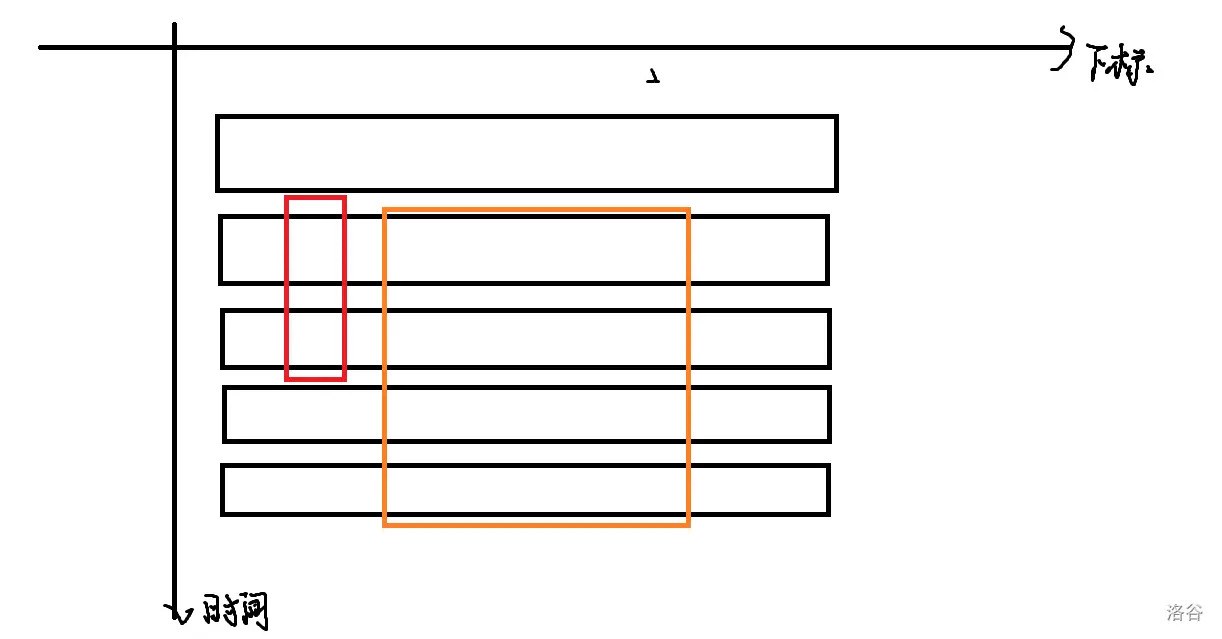
\includegraphics[width=10cm]{images/time.png}
\end{figure}
\par \noindent 把\textbf{初始数组按照时间轴赋值多份},于是最终认为:查询是查一个区间,但是修改是修改一个矩形(把当前时间到最后都会修改)。
~\\
\par \noindent 直接考虑离线询问,然后扫描线扫序列,然后数据结构维护时间维。
~\\
\par \noindent 考虑只有一个数的做法。 相当于要查询时间轴上有多少数 $≤K$ 
~\\
\par \noindent 离线然后按照时间分块,查询大块直接二分就行了(始终保持块内有序),散块暴力即可。

\begin{minted}{c++}
#include <bits/stdc++.h>
#define int long long
using namespace std;


const int N = 2e6;
int n, siz = 360, bel, q, num, cnt, ans[N], a[N], pos[N], LL[N], RR[N];
struct update {
    int x, tim, val;
    friend bool operator<(update x, update y) {
        return (x.x != y.x) ? x.x < y.x : x.tim < y.tim;
    }
} q1[N];
struct ask {
    int x, tim, val, id;
    friend bool operator<(ask x, ask y) {
        return (x.x != y.x) ? x.x < y.x : x.tim < y.tim;
    }
} q2[N];
int s[N], t[N], tag[N];
// t[] 维护块内有序
void rebuild(int L, int R) {
    for (int i = L; i <= R; i++) t[i] = s[i];
    sort(t + L, t + R + 1, greater<int>());
}
void change(int l, int r, int k) {
    l = max(l, 0ll);
    r = min(r, q);
    int pl = pos[l], pr = pos[r];
    if (pl == pr) {
        for (int i = l; i <= r; i++) s[i] += k;
        rebuild(LL[pl], RR[pl]);
        return;
    }
    // 大块懒标记
    for (int i = pl + 1; i <= pr - 1; i++) tag[i] += k;
    // 小块暴力 记得重构使得大块有序
    for (int i = l; i <= RR[pl]; i++) s[i] += k;
    rebuild(LL[pl], RR[pl]);
    
    for (int i = LL[pr]; i <= r; i++) s[i] += k;
    rebuild(LL[pl], RR[pl]);
}
int query(int l, int r, int k) {
    int pl = pos[l], pr = pos[r], cnt = 0;
    if (pl == pr) {
        for (int i = l; i <= r; i++)
            if (s[i] + tag[pl] >= k)
                cnt++;
        return cnt;
    }
    // 大块每块是有序的 二分求
    for (int i = pl + 1; i <= pr - 1; i++) {
        int l1 = LL[i], r1 = RR[i];
        while (l1 < r1) {
            int mid = l1 + r1 + 1 >> 1 ;
            if (t[mid] + tag[i] >= k)
                l1 = mid;
            else
                r1 = mid - 1;
        }
        if (t[l1] + tag[i] >= k) cnt += l1 - LL[i] + 1;
    }
    int L = LL[pr], R = RR[pl];
    for (int i = l; i <= R; i++) if (s[i] + tag[pl] >= k) cnt++;
    for (int i = L; i <= r; i++) if (s[i] + tag[pr] >= k) cnt++;
    return cnt;
}
signed main() {
    cin >> n >> q;
    for (int i = 1; i <= n; i++) cin >> a[i];
    for (int i = 1; i <= q; i++) {
        int op, l, r, x;
        cin >> op;
        if (op == 1) {
            cin >> l >> r >> x;
            q1[++cnt] = {l, i, x};
            q1[++cnt] = {r + 1, i, -x};
        }  else {
            cin >> l >> x;
            q2[++num] = {l, i, x, num};
        }
    }

    bel = (q + 1 - 1) / siz + 1;
    for (int i = 1; i <= bel; i++) {
        LL[i] = (i - 1) * siz + 1;
        RR[i] = min(i * siz, q + 1);
        for (int j = LL[i]; j <= RR[i]; j++) {
            pos[j] = i;
        }
    }
    //======================================= 时间轴分块
    sort(q1 + 1, q1 + cnt + 1);
    sort(q2 + 1, q2 + num + 1);
    memset(ans, -1, sizeof(ans));

    for (int i = 1, j = 1; i <= num; i++) {
        while ((q1[j].x < q2[i].x || (q1[j].x == q2[i].x && q1[j].tim < q2[i].tim)) && j <= cnt) {
            change(q1[j].tim + 1, q + 1, q1[j].val); // 不包括这一秒 在下一秒生效
            ++j;
        }
        ans[q2[i].id] = query(1, q2[i].tim, q2[i].val - a[q2[i].x]);
    }
    for (int i = 1; i <= q; i++)  if (ans[i] != -1) cout << ans[i] << "\n";
    return 0;
}
\end{minted}


% 位运算及其运用
\section{位运算及其运用}
\subsection{常见等式}
$$
a+b=(a|b)+(a\&b)\\
a\oplus b=(a|b)\oplus(a\&b) \\
a+b=(a\oplus b)+2×(a\&b) \\
$$
\subsection{位运算函数}

\par 由于这些函数是内建函数,经过了编译器的高度优化,运行速度十分快(有些甚至只需要一条指令)。这些函数都可以在函数名末尾添加 l 或 ll (如 \_\_builtin\_popcountll )来使参数类型变为 ( unsigned ) long 或 ( unsigned ) long long (返回值仍然是 int 类型)。
\begin{minted}{c++}
#pragma GCC target ("popcnt")          // 这条GCC指令可以让__builtin_popcount被编译器识别为一条指令。

int __builtin_ffs(int x)               // 返回 x 的二进制末尾最后一个 1 的位置
int __builtin_clz(unsigned int x)      // 返回 x 的二进制的前导 0 的个数。当 x 为 0 时,结果未定义。
int __builtin_ctz(unsigned int x)      // 返回 x 的二进制末尾连续 0 的个数。当 x 为 0 时,结果未定义。

int __builtin_clrsb(int x)             // 当 x 的符号位为 0 时返回 x 的二进制的前导 0 的个数减一
                                       // 否则返回 x 的二进制的前导 1 的个数减一
int __builtin_popcount(unsigned int x) // 返回 x 的二进制中 1 的个数。
int __builtin_parity(unsigned int x)   // 判断 x 的二进制中 1 的个数的奇偶性。
\end{minted}

\par 有时候希望求出一个数以二为底的对数,如果不考虑 0 的特殊情况,就相当于这个数二进制的位数 -1 ,而一个数 n 的二进制表示的位数可以使用 32-\_\_builtin\_clz(n) 表示,因此 31-\_\_builtin\_clz(n) 就可以求出 n 以二为底的对数。

\subsection{子集枚举}
\par \noindent 二进制枚举子集下面代码就是枚举的s的子集(二进制状态压缩)
\begin{minted}{c++}
for (int i = s; i; i = (i - 1) & s) {
    //i表示的就是s的子集
}
\end{minted}
\par \noindent $O(2^n)$ 求出子集质数的乘积
\begin{minted}{c++}
// vector<int> p(n) 有n个质数
std::vector<std::array<int, 2>> a(1 << n);
a[0] = {1, 1};
for (int i = 1; i < (1 << n); i++) {
    int j = __builtin_ctz(i);
    auto [x, y] = a[i ^ (1 << j)];
    a[i] = {x * p[j], -y};
}
\end{minted}

% C++ 高精度
\section{C++大整数模板}
\begin{minted}{c++}
const int maxn=110;
struct BigInt{
    int d[maxn], len;
 
    BigInt()          { memset(d, 0, sizeof(d)); len = 1; }
    BigInt(int num)   { *this = num; } 
    BigInt(char* num) { *this = num; }

    void clean() { while(len > 1 && !d[len-1]) len--; }
    BigInt operator = (const char* num){
        memset(d, 0, sizeof(d)); len = strlen(num);
        for(int i = 0; i < len; i++) d[i] = num[len-1-i] - '0';
        clean();
        return *this;
    }
    BigInt operator = (int num){
        char s[20];
        sprintf(s, "%d", num);
        *this = s;
        return *this;
    }
 
    BigInt operator + (const BigInt& b){
        BigInt c = *this; int i;
        for (i = 0; i < b.len; i++){
            c.d[i] += b.d[i];
            if (c.d[i] > 9) c.d[i] %= 10, c.d[i+1]++;
        }
        while (c.d[i] > 9) c.d[i++] %= 10, c.d[i]++;
        c.len = max(len, b.len);
        if (c.d[i] && c.len <= i) c.len = i+1;
        return c;
    }
    BigInt operator - (const BigInt& b){
        BigInt c = *this; int i;
        for (i = 0; i < b.len; i++){
            c.d[i] -= b.d[i];
            if (c.d[i] < 0) c.d[i] += 10, c.d[i+1]--;
        }
        while (c.d[i] < 0) c.d[i++] += 10, c.d[i]--;
        c.clean();
        return c;
    }
    BigInt operator * (const BigInt& b)const{
        int i, j; 
        BigInt c;
        c.len = len + b.len; 
        for(j = 0; j < b.len; j++)
            for(i = 0; i < len; i++) 
                c.d[i+j] += d[i] * b.d[j];
        for(i = 0; i < c.len-1; i++)
            c.d[i+1] += c.d[i] / 10, c.d[i] %= 10;
        c.clean();
        return c;
    }
    BigInt operator / (const BigInt& b){
        int i, j;
        BigInt c = *this, a = 0;
        for (i = len - 1; i >= 0; i--) {
            a = a * 10 + d[i];
            for (j = 0; j < 10; j++)
                if (a < b*(j+1))
                    break;
            c.d[i] = j;
            a = a - b*j;
        }
        c.clean();
        return c;
    }
    BigInt operator % (const BigInt& b){
        int i, j;
        BigInt a = 0;
        for (i = len - 1; i >= 0; i--) {
            a = a * 10 + d[i];
            for (j = 0; j < 10; j++) if (a < b*(j+1)) break;
            a = a - b*j;
        }
        return a;
    }
    BigInt operator += (const BigInt& b){
        *this = *this + b;
        return *this;
    }
 
    bool operator < (const BigInt& b) const{
        if(len != b.len)
            return len < b.len;
        for(int i = len-1; i >= 0; i--)
            if(d[i] != b.d[i])
                return d[i] < b.d[i];
        return false;
    }
    bool operator >  (const BigInt& b) const{return b < *this;}
    bool operator <= (const BigInt& b) const{return !(b < *this);}
    bool operator >= (const BigInt& b) const{return !(*this < b);}
    bool operator != (const BigInt& b) const{return b < *this || *this < b;}
    bool operator == (const BigInt& b) const{return !(b < *this) && !(b > *this);}
 
    string str() const{
        char s[maxn]={};
        for(int i = 0; i < len; i++)
            s[len-1-i] = d[i]+'0';
        return s;
    }
};
 
istream& operator >> (istream& in, BigInt& x) {
    string s;
    in >> s;
    x = s.c_str();
    return in;
}
 
ostream& operator << (ostream& out, const BigInt& x) {
    out << x.str();
    return out;
}
\end{minted}

% 快速读入、__int128、开栈、随机
\section{FastIO}

\begin{minted}{c++}
#pragma GCC optimize(2)
#pragma GCC optimize(3)
#pragma GCC optimize("Ofast")
// 整数读入 (int, ll)
template<class T> void read(T &x) {
    T a = 0, f = 1;
    char ch = getchar();
    while (ch < '0' || ch > '9')
        f = ch == '-' ? -1 : f, ch = getchar();
    while (ch >= '0' && ch <= '9')
        a = a * 10 + ch - '0', ch = getchar();
    x = a * f;
}
// 浮点数读入
inline double read() {
    double x = 0, y = 1.0;
    int f = 0;
    char ch = getchar();
    while (!isdigit(ch))
        f |= ch == '-', ch = getchar();
    while (isdigit(ch))
        x = x * 10 + (ch ^ 48), ch = getchar();
    ch = getchar();
    while (isdigit(ch))
        x += (y /= 10) * (ch ^ 48), ch = getchar();
    return f ? -x : x;
}
//=============================究极快读
#include<bits/stdc++.h>
using namespace std;
namespace nqio {
    const unsigned R = 4e5, W = 4e5;
    char *a, *b, i[R], o[W], *c = o, *d = o + W, h[40], *p = h, y;
    bool s;
    struct q {
        void r(char &x) { x = a == b && (b = (a = i) + fread(i, 1, R, stdin), a == b) ? -1 : *a++;}
        void f() { fwrite(o, 1, c - o, stdout);c = o;}
        ~q() { f();}
        void w(char x) { *c = x; if (++c == d) f(); }
        q &operator>>(char &x) { do r(x); while (x <= 32); return*this;}
        q &operator>>(char *x) { do r(*x);while (*x <= 32); while (*x > 32) r(*++x); *x = 0; return*this;}
        
        template<typename t>
        q &operator>>(t &x) {
            for (r(y), s = 0; !isdigit(y); r(y)) s |= y == 45;
            if (s) for (x = 0; isdigit(y); r(y)) x = x * 10 - (y ^ 48);
            else   for (x = 0; isdigit(y); r(y)) x = x * 10 + (y ^ 48);
            return*this;
        }
        q &operator<<(char x) { w(x); return*this; }
        q &operator<<(char *x) { while (*x) w(*x++); return*this; }
        q &operator<<(const char *x) { while (*x) w(*x++); return*this; }
        
        template<typename t>
        q &operator<<(t x) {
            if (!x) w(48);
            else if (x < 0) for (w(45); x; x /= 10) * p++ = 48 | -(x % 10);
            else for (; x; x /= 10) * p++ = 48 | x % 10;
            while (p != h) w(*--p);
            return*this;
        }
    } qio;
} using nqio::qio;

int main()
{
    __int128 a,b;
    qio >> a >> b;
    qio << a + b<< '\n';
    return 0;
}
\end{minted}
\section{\_\_int128 输出函数}
\begin{minted}{c++}
void output(__int128 x) {
    if (!x)
        return;
    if (x < 0)
        putchar('-'), x = -x;
    output(x / 10);
    putchar(x % 10 + '0');
}
\end{minted}

\section{开栈}
\par \noindent Tips: 并不是在所有的地方都能用。一定要最后写一句 exit(0); 退出程序。
\begin{minted}{c++}
//64−bit
int size = 1 << 20;     //256M
char *p = (char *)malloc(size) + size;
__asm__("movq %0, %%rsp\n" :: "r"(p));

//32−bit
int size = 1 << 20;     //256M
char *p = (char *)malloc(size) + size;
__asm__("movl %0, %%esp\n":: "r"(p));

// 内存屏障
asm volatile("" ::: "memory");
__asm__ __volatile__ ("" ::: "memory");
\end{minted}
\section{随机}
\begin{itemize}
\item 不要使⽤ rand()。

\item chrono::steady\_clock::now().time\_since\_epoch().count() 可⽤于计时。

\item 64位可以使⽤ mt19937\_64。
\end{itemize}
\begin{minted}{c++}
int main() {
    
    const int N=1000010;
    mt19937 rng(chrono::steady_clock::now().time_since_epoch().count());
    
    vector<int> permutation(N);
    
    for (int i = 0; i < N; i++) permutation[i] = i;
    
    shuffle(permutation.begin(), permutation.end(), rng);
    
    for (int i = 0; i < N; i++) permutation[i] = i;
    
    for (int i = 1; i < N; i++) swap(permutation[i], permutation[uniform_int_distribution<int>(0, i)(rng)]);
}
//============ 真实随机数
mt19937 mt(time(0));
auto rd = bind(uniform_real_distribution<double>(0, 1), mt);
auto rd2 = bind(uniform_int_distribution<int>(1, 6), mt);
\end{minted}

% 对拍
\section{对拍}

\subsection{生成随机数据}

\begin{minted}{c++}
#include <iostream>
#include <cstdlib>
#include <ctime>
using namespace std;
int random(int n) { //生成一个[0,n-1]范围内的数
    return (long long)rand() * rand() % n;
}
int main() {
    srand((unsigned)time(0));
    // ===========随机生成排列===========
    int n = random(100000) + 1, a[100050];

    for (int i = 1; i <= n; i++)
        a[i] = i;

    random_shuffle(a + 1, a + n + 1); //库文件algorithm

    for (int i = 1; i <= n; i++)
        printf("%d ", a[i]);

    //===========随机生成m个[1,n]的子区间===========
    for (int i = 1; i <= m; i++) {
        int l = random(n) + 1;
        int r = random(n) + 1;

        if (l > r)
            swap(l, r);

        printf("%d %d\n", l, r);
    }

    //===========随机生成一棵n个点带边权(<=100000)的树===========
    for (int i = 2; i <= n; i++) {
        int fa = random(i - 1) + 1;
        int val = random(100000) + 1;
        printf("%d %d %d\n", fa, i, val);
    }

    //随机生成一张n个点,m条边的无向图.
    pair<int, int> e[]; //[]内填写数组大小
    map<pair<int, int>, bool> h; //库文件map
    //先生成一棵树,保证联通

    int n = random(具体大小), m = random(具体大小);
    printf("%d %d\n", n, m);

    for (int i = 1; i < n; i++) {
        int fa = random(i) + 1;
        e[i] = make_pair(fa, i + 1);
        h[e[i]] = h[make_pair(i + 1, fa)] = 1;
    }

    //在生成剩余的m-n+1条边
    for (int i = n; i <= n; i++) {
        int x, y;

        do {
            x = random(n) + 1, y = random(n) + 1;
        } while (x == y || h[make_pair(x, y)]);

        e[i] = make_pair(x, y);
        h[e[i]] = h[make_pair(y, x)] = 1;
    }

    //随机打乱,输出
    random_shuffle(e + 1, e + m + 1); //库文件algorithm

    for (int i = 1; i <= m; i++)
        printf("%d %d\n", e[i].first, e[i].second);

    //===========生成一条有n个节点的链===========
    int n = random(1000) + 1;
    printf("%d\n", &n);
    int root = random(n) + 1;
    bool vis[100000];
    vis[root] = 1;
    int last = root;

    for (int i = 1; i < n; i++) {
        int x = random(n) + 1;

        while (vis[x] == 1)
            x = random(n) + 1;

        printf("%d %d\n", last, x);
        last = x;
        vis[x] = 1;
    }

    //===========生成一条有n个节点的菊花图===========
    int n = random(1000) + 1;
    printf("%d\n", n);
    int root = random(n) + 1;

    for (int i = 1; i <= n; i++) {
        if (i == root)
            continue;

        printf("%d %d\n", root, i);
    }

    return 0;
}
\end{minted}

\subsection{Windows下的批处理}

\par \noindent 用文本编辑器(记事本就行)写好,保存为.bat 后缀名
\begin{minted}{c++}
@echo off                               //关掉输入显示,否则所有的命令也会显示出来
:loop                                   //生成随机输入
    rand.exe > in.txt
    my.exe < in.txt  > out.txt       
    std.exe < in.txt  > stdout.txt
    fc out.txt stdout.txt               //比较文件
    if not errorlevel 1   goto loop     //不为1继续循环,fc在文件相同时返回0,不同时返回1
pause                                   //不同时暂停,你可以看in.txt里的数据
goto loop                               //看完数据,按任意键结束暂停,继续循环
\end{minted}

\subsection{Linux下的Bash脚本}

\par \noindent 同样用文本编辑器写好保存为.sh(例如cmp.sh),在执行chmod +x cmp.sh,即可用./cmp.sh来执行它,当然扩展名也不是必需的,完全可以用不带扩展名的cmp命名。
\begin{minted}{c++}
#!/bin/bash
while true; do
    ./r > input                         //生成随机事件
    ./a < input > output.a
    ./b < input > output.b
    diff output.a output.b           //文本比较
    if [ $? -ne 0 ] ; then break;fi     //判断返回值
done
\end{minted}




% 其他

\section{其他}
\begin{itemize}
\item 将一个点 $(x,y)$ 的坐标变为 $(x+y,x−y)$ 后,原坐标系中的曼哈顿距离 $=$ 新坐标系中的切比雪夫距离

\item 将一个点 $(x,y)$ 的坐标变为 $(\frac{x+y}{2},\frac{x−y}{2})$ 后,原坐标系中的切比雪夫距离 $=$ 新坐标系中的曼哈顿距离
\end{itemize}


%% 附录
%\chapter{网络流/二分图/匹配}

% 二分图匹配
\section{二分图}
\subsection{匈牙利算法}
\par \noindent 考虑点集A,B二分图
\par \noindent \textbf{最小点覆盖}:
\par \noindent 概念:用最少的点覆盖二分图中所有边。
\par \noindent 结论:最小覆盖点=最大匹配
\par \noindent 
\par \noindent \textbf{最小边覆盖}:
\par \noindent 概念:用最少的边覆盖点集A,B中的所有点。
\par \noindent 结论:最小边覆盖=总点数-最大匹配
\par \noindent 
\par \noindent \textbf{最大独立集}
\par \noindent 概念:选出最多的点使得点集内部没有边。
\par \noindent 结论:最大独立集=总点数-最大匹配
\par \noindent 
\par \noindent \textbf{最小路径点覆盖}
\par \noindent 概念:对于一个有向图,选出最少的不相交路径使其覆盖所有点。
\par \noindent 结论:最小路径覆盖=总点数-最大匹配
\par \noindent 
\par \noindent \textbf{最小路径重复点覆盖}
\par \noindent 概念:对于一个有向图,选出最少的(能相交)路径使其覆盖所有点。
\par \noindent 结论:对原图求传递闭包之后再对新图求最小不相交路径覆盖

\begin{minted}{c++}
int match[manx], vis[manx];
bool dfs(int x) {
// 遍历 x 的每条出边
    for (int i = h[x], y; i != -1; i = ne[i]) {
        y = e[i];
        // 如果在当前递归 DFS 的过程中,y 没有被访问过
        if (!vis[y]) {
            vis[y] = 1; // 先将 y 分配给 x, 标记 y 被访问
        // 如果 y 没有被匹配,那就让它与 x 匹配
        // 否则,尝试对 y 已匹配的边匹配其他的节点,然后再让 y 与 x 匹配
        if (!match[y] || dfs(match[y])) {
                match[y] = x;
                return true;
            }
        }
    }
    // 如果走到了这里,说明该点匹配失败
    return false;
}
int main() {
    int ans = 0;
    for (int i = 1; i <= n; i++) {
    // 重设 vis 数组,表示所有点都不在增广路中
        memset(vis, 0, sizeof vis);
    // 尝试为每个点匹配(找增广路),如果匹配成功则 ans++
    if (dfs(i)) ans++;
    }
}
\end{minted}

\subsection{KM算法}
\par \noindent 解决二分图最大带权匹配,时间复杂度 $O(n^3)$.
\begin{minted}{c++}
#include<cstdio>
#include<cstring>
#include<iostream>
#include<algorithm>
using namespace std;
typedef long long ll;
const int N=510;
ll w[N][N],lx[N],ly[N];//顶标
bool visx[N],visy[N];//记录是否在交错树上
int match[N];//匹配
int n,m,p[N];
ll delta,c[N];//delta和更新后的delta
void bfs(int x)
{
    int a,y=0,y1=0;
    for(int i=1;i<=n;i++) p[i]=0,c[i]=1e18;
    match[y]=x;
    do{
        a=match[y],delta=1e18,visy[y]=1;
        for(int b=1;b<=n;b++)
            if(!visy[b])
            {
                if(c[b]>lx[a]+ly[b]-w[a][b])
                    c[b]=lx[a]+ly[b]-w[a][b],p[b]=y;
                if(c[b]<delta)//Δ还是取最小的
                    delta=c[b],y1=b;
            }
        for(int b=0;b<=n;b++)
            if(visy[b])
                lx[match[b]]-=delta,ly[b]+=delta;
            else
                c[b]-=delta;
        y=y1;
    }while(match[y]);
    while(y) match[y]=match[p[y]],y=p[y];
}
ll KM()
{
    for(int i=1;i<=n;i++)
        match[i]=lx[i]=ly[i]=0;
    for(int i=1;i<=n;i++)
    {
        memset(visy,0,sizeof visy);
        bfs(i);
    }
    
    ll res=0;
    for(int i=1;i<=n;i++)
        res+=w[match[i]][i];
    return res;
}
int main()
{
    scanf("%d%d",&n,&m);
    for(int i=1;i<=n;i++)
        for(int j=1;j<=n;j++) 
            w[i][j]=-1e18;
    for(int i=1;i<=m;i++)
    {
        int a,b;ll c;
        scanf("%d%d%lld",&a,&b,&c);
        w[a][b]=max(w[a][b],c);
    }
    printf("%lld\n",KM());
    for(int i=1;i<=n;i++)
        printf("%d ",match[i]);
    puts("");
    return 0;
}
\end{minted}

\subsection{染色判二分图}
\begin{minted}{c++}
int vis[MAXN], flag = 1;
void dfs(int x, int co) {
    vis[x] = co;
    for (int i = h[x]; i != -1; i = ne[i]) {
        if (vis[e[i]] == 0)
            dfs(vis[e[i]], 3 - co); // 注意这里的小技巧,3-1=2, 3-2=1.
        else if (vis[e[i]] == co) {
            flag = 0;
            return;
        }
    }
}
for (int i = 0; i < n; i++) {
    if (!vis[i] && flag)
        dfs(i, 1);
    if (!flag) break;
}
printf(flag ? "Yes" : "No");
\end{minted}
\clearpage

% 最大流
\section{最大流}

\subsection{Dinic 算法 (带当前弧优化)}

\par 不断在残量图上使用 BFS 求出结点的层次,构建分层图(即给结点标注 d[i]);然后在分层图上 DFS 寻找增广路,回溯时实时更新剩余容量。每个点可以流向多条出边。时间复杂度为 $O(n^2m)$。
\begin{minted}{c++}
template <int N> struct Dinic {
    const int INF = 1e9;
    struct E {
        int to, cap, rev;// x->y 目标点 to=y 流量cap 反向边G[to][rev]=x
    };
    vector<E> G[N];
    int lev[N], cur[N];// 层数 当前弧优化
    inline void add(int x, int y, int c) {
        G[x].push_back({ y, c, (int)G[y].size() });
        G[y].push_back({ x, 0, (int)G[x].size() - 1 });
    }
    void bfs(int s) {
        queue<int> q;
        memset(lev, -1, sizeof lev);

        for (lev[s] = 0, q.push(s); q.size();) {
            int x = q.front();
            q.pop();

            for (auto &e : G[x])
                if (e.cap > 0 && lev[e.to] < 0)// 层数未赋值 容量大于0
                    lev[e.to] = lev[x] + 1, q.push(e.to);
        }
    }
    int dfs(int x, int t, int f) {
        if (x == t)
            return f;
        // 当前弧优化
        for (int &i = cur[x], sz = G[x].size(), d; i < sz; i++) {
            auto &e = G[x][i];

            if (e.cap > 0 && lev[x] < lev[e.to]) {// lev[e.to]==lev[x]+1
                if ((d = dfs(e.to, t, min(f, e.cap))) > 0) {
                    e.cap -= d, G[e.to][e.rev].cap += d;// 正向边流量-d 反向边容量+d
                    return d;
                }
            }
        }

        return 0;
    }
    int64_t maxflow(int s, int t) {
        for (int64_t flow = 0, f;;) {
            bfs(s);

            if (lev[t] < 0)// BFS未遍历到终点
                return flow;

            memset(cur, 0, sizeof cur);// 当前弧指向第一条边即G[x][0]

            while ((f = dfs(s, t, INF)) > 0)
                flow += f;
        }
    }
};
Dinic<10010> din;
\end{minted}

\subsection{无源汇上下界可行流}
\par \textbf{问题:} 给定一个网络,求一个流满足:每条边的流量处在给定的下界和上界 [lower,upper] 之间,满足流量守恒

\begin{itemize}
\item 记$A(u)=\sum_{to [i]=u}f(i)-\sum_{from[i]=u}f(i)$即流入减去流出
\item 若$A(u)>0$,源点 $S$ 向 $u$ 点连边,容量是$A(u)$
\item 若$A(u)<0$,$u$ 点向汇点 $T$ 连边,容量是$-A(u)$
\end{itemize}
如果\textbf{满流}(虚拟源点 S 流跑满)此时即可求出流2(否则无解),再加上流1即是满足题意的可行流
\begin{minted}{c++}
int main() {

    cin >> n >> m;
    S = 0, T = n + 1; // 虚拟源点 汇点
    for (int i = 1; i <= m; i++) {
        int x, y, c, d; cin >> x >> y >> c >> d;
        din.add(x, y, d - c, i);
        in[y] += c, out[x] += c;
        l[i] = c;
    }
    int sum = 0;
    for (int i = 1; i <= n; i++) {
        if (in[i] > out[i])
            din.add(S, i, in[i] - out[i], 0), sum += in[i] - out[i]; // 满流
        else
            din.add(i, T, out[i] - in[i], 0);
    }
    if (sum != din.maxflow(S, T))
        cout << "NO\n";
    else {
        cout << "YES\n";
        for (int x = 1; x <= n; x++)
            for (auto [y, cap, rev, id] : din.G[x]) {
                ans[id] = cap;
            }
        for (int i = 1; i <= m; i++)
            cout << ans[i] + l[i] << '\n';
    }
    return 0;
}
\end{minted}
\subsection{有源汇上下界最大流}
\par \noindent 连接一条 $t\to s$下界是 0 上界是 $\infty$ 的边,由此转化循环流问题(无源汇上下界可行流)
\par \noindent 
\par \noindent 按照循环流问题建图,首先跑 $S \to T$ 的dinic 是否能够找到一条可行流(即判断是否是满流)然后在换源点和汇点并删去 $t\to s$ 的边再跑一边 $s\to t$ dinic(榨干残留网络),可行流 + 第二次dinic即是最大流
\begin{minted}{c++}
int main() {

    // ............. 无源汇上下界可行流建图
    din.add(t, s, 1e9);

    res = din.maxflow(S, T);

    if (res != sum) {
        cout << "No Solution\n";
        return 0;
    }
    auto &[v, cap, inv] = din.G[s].back();
    res = cap;
    din.erase(din.G[v][inv]); //删去 t->s 容量是1e9这条边
    cout << res + din.maxflow(s, t);
    return 0;
}
\end{minted}

\subsection{有源汇上下界最小流}
\par \noindent 最小流 = 可行流 + $s\to t$ 流,由于可行流固定,为了使结果最小即 $s\to t$ 流最小,由于 $s\to t$ 的流 = $- t\to s$的流,如果 $t\to s$ 求最大流,那么 $s\to t$ 就是最小流,$f_{s\to t}=-f_{t\to s}$ 这也是为什么相减的原因。
\begin{minted}{c++}
int main() {
    
    // ............. 无源汇上下界可行流建图
    din.add(t, s, 1e9);

    res = din.maxflow(S, T);

    if (res != sum) {
        cout << "No Solution\n";
        return 0;
    }

    auto &[v, cap, inv] = din.G[s].back();
    res = cap;
    din.erase(din.G[v][inv]); //删去 t->s 容量是1e9这条边

    cout << res - din.maxflow(t, s); // f(s->t) = - f(t->s)
    return 0;
}
\end{minted}


% 最小费用最大流
\section{最小费用最大流}
\subsection{Primal-Dual 原始对偶算法}
\par 给定一个网络 $G=(V, E)$,每条边 $(u, v) \in E$ 带有属性 $c(u, v)$,表示从当前边流过 1 个单位流量时的费用。在最大化流量的基础上,求最小的费用。

\begin{minted}{c++}
#include <bits/stdc++.h>
#define int long long
#pragma GCC optimize(2)
using namespace std;
const int inf=1e9;
template <int N> struct MCMF {
    struct E {
        int to, cap, val, inv;
    };
    vector <E> G[N];
    int lev[N], cur[N], h[N], pre[N], preu[N];
    void add(int u, int v, int f, int w) {
        G[u].push_back({v, f, w, (int)G[v].size()});
        G[v].push_back({u, 0, -w, (int)G[u].size() - 1});
    }
    void dijkstra(int st) {
        priority_queue<pair<int, int>, vector<pair<int, int>>, greater<pair<int, int>>>q;
        memset(lev, 0x3f, sizeof lev);
        memset(pre, -1, sizeof pre);
        memset(preu, -1, sizeof preu);
        lev[st] = 0;
        q.push({0, st});

        while (q.size()) {
            auto [d, u] = q.top();
            q.pop();

            if (lev[u] < d) continue;

            int x = 0;

            for (auto [v, f, w, inv] : G[u]) {
                if (f && lev[v] > lev[u] + w + h[u] - h[v]) {
                    lev[v] = lev[u] + h[u] - h[v] + w;
                    pre[v] = x;
                    preu[v] = u;
                    q.push({lev[v], v});
                }
                x++;
            }
        }
    }
    pair<int, int> min_cost_max_flow(int st, int ed) {
        memset(h, 0, sizeof h);

        for (int flow = 0, cost = 0, res = inf;; res = inf) {

            dijkstra(st);

            if (lev[ed] > inf)
                return {flow, cost};

            for (int i = 0; i < N; i++) {
                h[i] += lev[i];
            }

            for (int i = ed; i != st; i = preu[i]) {
                res = min(res, G[preu[i]][pre[i]].cap);
            }

            flow += res;
            cost += res * h[ed];

            for (int i = ed; i != st; i = preu[i]) {
                G[i][G[preu[i]][pre[i]].inv].cap += res;
                G[preu[i]][pre[i]].cap -= res;
            }
        }
    }
};

MCMF<5005>mcmf;
int n, m, s, t;

signed main() {
    ios::sync_with_stdio(false);
    cin.tie(0);
    cout.tie(0);
    cin >> n >> m >> s >> t;

    for (int i = 1; i <= m; i++) {
        int u, v, w, c;
        cin >> u >> v >> w >> c;
        mcmf.add(u, v, w, c);
    }

    auto [f, c] = mcmf.min_cost_max_flow(s, t);
    cout << f << " " << c << '\n';
}
\end{minted}

\subsection{EK算法求最大流}

\begin{minted}{c++}
#include <queue>
#include <iostream>
#include <cstring>
#include <algorithm>
using namespace std;
const int N = 5010, M = 100010;
int h[N], e[M], ne[M], f[M], w[M], idx;
int d[N], flow[N], pre[N];
bool st[N];
queue<int> q;

void add(int a, int b, int c, int d) {
    e[idx] = b, f[idx] = c, w[idx] = d, ne[idx] = h[a], h[a] = idx++;
    e[idx] = a, f[idx] = 0, w[idx] = -d, ne[idx] = h[b], h[b] = idx++;
}
bool spfa(int s, int t) {
    memset(d, 0x3f, sizeof d);
    memset(flow, 0, sizeof flow);
    d[s] = 0, flow[s] = 0x3f3f3f3f;
    q.push(s);

    while (q.size()) {
        int u = q.front();
        q.pop();
        st[u] = 0;

        for (int i = h[u]; i != -1; i = ne[i]) {
            int v = e[i];

            if (f[i] && d[v] > d[u] + w[i]) {
                d[v] = d[u] + w[i];
                pre[v] = i;
                flow[v] = min(f[i], flow[u]);

                if (!st[v]) {
                    q.push(v);
                    st[v] = 1;
                }
            }
        }
    }

    return flow[t] > 0;
}
pair<int, int> EK(int s, int t) {
    int maxflow = 0, mincost = 0;

    while (spfa(s, t)) {
        int r = flow[t];
        maxflow += r, mincost += r * d[t];

        for (int i = t; i != s; i = e[pre[i] ^ 1]) {
            f[pre[i]] -= r;
            f[pre[i] ^ 1] += r;
        }
    }

    return make_pair(maxflow, mincost);
}
int n, m, s, t;
int main() {
    cin >> n >> m >> s >> t;
    memset(h, -1, sizeof h);

    while (m--) {
        int a, b, c, d;
        cin >> a >> b >> c >> d;
        add(a, b, c, d);
    }

    auto [maxflow, mincost] = EK(s, t);

    cout << maxflow << ' ' << mincost << '\n';
    return 0;
}
\end{minted}
 
\end{document}
